% defer/defer.tex
% SPDX-License-Identifier: CC-BY-SA-3.0

\QuickQuizChapter{chp:Deferred Processing}{Deferred Processing}
%
\Epigraph{All things come to those who wait.}{\emph{Violet Fane}}

일을 뒤로 미루는 전략은 기록된 역사의 시작 전까지 이어져 있습니다.
이것은 자주 미루기나 완전한 게으름으로 여겨져 비웃음을 받아왔습니다.
하지만, 지난 수십년간 사람들은 병렬 알고리즘들의 단순화와 능률화에 있어서의 이
전략의 가치를 깨달았습니다~\cite{Kung80,HMassalinPhD}.
이걸 믿든 믿지 않든, 병렬 프로그래밍에서의 ``게으름'' 은 종종 근면성에 비해
성능과 확장성이 좋습니다!
이런 성능과 확장성에서의 장점은 일을 뒤로 미루는 것은 종종 동기화 기능들을
약화시키는게 가능하게 하고, 따라서 동기화 오버헤드를 줄이게 된다는 사실에서
기인합니다.
일을 뒤로 미루는 일반적인 전략은
레퍼런스 카운팅 (Section~\ref{sec:defer:Reference Counting}),
해저드 포인터 (Section~\ref{sec:defer:Hazard Pointers}),
순차적 락킹 (Section~\ref{sec:defer:Sequence Locks}),
그리고 RCU (Section~\ref{sec:defer:Read-Copy Update (RCU)}) 등을 포함합니다.
마지막으로, Section~\ref{sec:defer:Which to Choose?}
에서는 이 챕터에서 다루어진 일 뒤로 미루기 전략들 가운데 어떻게 선택을 해야
하는지 이야기 하고, 
Section~\ref{sec:defer:What About Updates?} 에서는 업데이트의 역할에 대해
논합니다.
\iffalse

The strategy of deferring work goes back before the dawn of recorded
history. It has occasionally been derided as procrastination or
even as sheer laziness.
However, in the last few decades workers have recognized this strategy's value
in simplifying and streamlining parallel algorithms~\cite{Kung80,HMassalinPhD}.
Believe it or not, ``laziness'' in parallel programming often outperforms and
out-scales industriousness!
These performance and scalability benefits stem from the fact that
deferring work often enables weakening of synchronization primitives,
thereby reducing synchronization overhead.
General approaches of work deferral include
reference counting (Section~\ref{sec:defer:Reference Counting}),
hazard pointers (Section~\ref{sec:defer:Hazard Pointers}),
sequence locking (Section~\ref{sec:defer:Sequence Locks}),
and RCU (Section~\ref{sec:defer:Read-Copy Update (RCU)}).
Finally, Section~\ref{sec:defer:Which to Choose?}
describes how to choose among the work-deferral schemes covered in
this chapter and Section~\ref{sec:defer:What About Updates?}
discusses the role of updates.
\fi

하지만 먼저 이런 방법들을 비교하고 대비하는데에 사용될 예제 알고리즘을
소개하겠습니다.
\iffalse

But first we will introduce an example algorithm that will be used
to compare and contrast these approaches.
\fi

\section{Running Example}
\label{sec:defer:Running Example}

이 챕터는 이런 접근법들의 가치를 보이고 또 그것들을 서로 비교할 수 있도록 하기
위해 단순화된 패킷 라우팅 알고리즘을 사용할 겁니다.
라우팅 알고리즘은 운영체제 커널에서 각각의 바깥으로 나가는 TCP/IP 패킷들을
알맞는 네트워크 인터페이스로 전달하는데에 사용됩니다.
이 특정한 알고리즘은 고전적인 1980년대의 packet-train-optimized 알고리즘으로
BSD UNIX~\cite{VanJacobson88} 에서 사용되었으며, 단순한 링크드 리스트로
구성되었습니다.\footnote{
	달리 말하자면, 이건 OpenBSD, NetBSD 도 아니고 심지어 FreeBSD 도
	아니었고 Pre-BSD 였습니다.}
최신 라우팅 알고리즘들은 더 복잡한 데이터 구조를 사용합니다만,
Chapter~\ref{chp:Counting} 에서와 같이, 극단적으로 간단한 알고리즘이 극단적으로
이해하기 쉬운 구성에서의 병렬성에 특정된 문제들을 밝히는데 도움을 줄 것입니다.
\iffalse

This chapter will use a simplified packet-routing algorithm to demonstrate
the value of these approaches and to allow them to be compared.
Routing algorithms are used in operating-system kernels to
deliver each outgoing TCP/IP packets to the appropriate network interface.
This particular algorithm is a simplified version of the classic 1980s
packet-train-optimized algorithm used in BSD UNIX~\cite{VanJacobson88},
consisting of a simple linked list.\footnote{
	In other words, this is not OpenBSD, NetBSD, or even
	FreeBSD, but none other than Pre-BSD.}
Modern routing algorithms use more complex data structures, however, as in
Chapter~\ref{chp:Counting}, a simple algorithm will
help highlight issues specific to parallelism in an
easy-to-understand setting.
\fi

우리는 더 나아가서 출발지와 목적지 IP 주소와 포트들 네가지 정보로 구성되는 검색
키를 간단한 정수로 교체함으로써 알고리즘을 더욱 단순화할 겁니다.
검색되고 리턴되는 값 또한 간단한 정수로 바꿔질 것이어서, 데이터 구조는
Figure~\ref{fig:defer:Pre-BSD Packet Routing List} 에서와 같이 될건데,
이 그림대로라면 address~42 의 패킷을 interface~1 로, address~56 의 패킷을
interface~2 로, 그리고 address~17 의 패킷을 interface~7 로 전달할 겁니다.
외부의 패킷 네트워크는 안정적일 것을 가정하면, 이 리스트는 매우 자주 검색되고
아주 가끔씩만 업데이트 될 것입니다.
Chapter~\ref{chp:Hardware and its Habits} 에서 우리는, 빛의 제한된 속도와
물질의 원자성의 자연적 법칙과 같은 불편한 물리 법칙을 회피하는 가장 좋은 방법은
데이터를 쪼개거나 읽기가 대부분인 공유에 기대는 것임을 배웠습니다.
이 챕터에서, 우리는 이 Pre-BSD 패킷 라우팅 리스트를 사용해 읽기가 대부분인
상황을 위한 동기화 기법을 평가해 보도록 하겠습니다.
\iffalse

We further simplify the algorithm by reducing the search key from
a quadruple consisting of source and destination IP addresses and
ports all the way down to a simple integer.
The value looked up and returned will also be a simple integer,
so that the data structure is as shown in
Figure~\ref{fig:defer:Pre-BSD Packet Routing List}, which
directs packets with address~42 to interface~1, address~56 to
interface~3, and address~17 to interface~7.
Assuming that external packet network is stable,
this list will be searched frequently and updated rarely.
In Chapter~\ref{chp:Hardware and its Habits}
we learned that the best ways to evade inconvenient laws of physics, such as
the finite speed of light and the atomic nature of matter, is to
either partition the data or to rely on read-mostly sharing.
In this chapter, we will use this Pre-BSD packet routing
list to evaluate a number of read-mostly synchronization techniques.
\fi

\begin{figure}[tb]
\begin{center}
\resizebox{3in}{!}{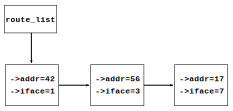
\includegraphics{defer/RouteList}}
\end{center}
\caption{Pre-BSD Packet Routing List}
\label{fig:defer:Pre-BSD Packet Routing List}
\end{figure}

\begin{listing}[tb]
{ \scriptsize
\begin{verbbox}
 1 struct route_entry {
 2   struct cds_list_head re_next;
 3   unsigned long addr;
 4   unsigned long iface;
 5 };
 6 CDS_LIST_HEAD(route_list);
 7
 8 unsigned long route_lookup(unsigned long addr)
 9 {
10   struct route_entry *rep;
11   unsigned long ret;
12
13   cds_list_for_each_entry(rep,
14                           &route_list, re_next) {
15     if (rep->addr == addr) {
16       ret = rep->iface;
17       return ret;
18     }
19   }
20   return ULONG_MAX;
21 }
22
23 int route_add(unsigned long addr,
24               unsigned long interface)
25 {
26   struct route_entry *rep;
27
28   rep = malloc(sizeof(*rep));
29   if (!rep)
30     return -ENOMEM;
31   rep->addr = addr;
32   rep->iface = interface;
33   cds_list_add(&rep->re_next, &route_list);
34   return 0;
35 }
36
37 int route_del(unsigned long addr)
38 {
39   struct route_entry *rep;
40
41   cds_list_for_each_entry(rep,
42                           &route_list, re_next) {
43     if (rep->addr == addr) {
44       cds_list_del(&rep->re_next);
45       free(rep);
46       return 0;
47     }
48   }
49   return -ENOENT;
50 }
\end{verbbox}
}
\centering
\theverbbox
\caption{Sequential Pre-BSD Routing Table}
\label{lst:defer:Sequential Pre-BSD Routing Table}
\end{listing}

Figure~\ref{fig:defer:Sequential Pre-BSD Routing Table} 는
Figure~\ref{fig:defer:Pre-BSD Packet Routing List} 에 연관되는 간단한 싱글
쓰레드 구현을 보입니다.
Line~1-5 는 \co{route_entry} 구조체를 정의하고 line~6 는 \co{route_list} 헤더를
정의합니다.
Line~8-21 은 \co{route_lookup()} 을 정의하는데, 이 함수는 순차적으로
\co{route_list} 를 검색하고 검색에 성공하면 연관되는 \co{->iface} 를 리턴하고,
검색에 실패하면 \co{ULONG_MAX} 를 리턴합니다.
Line~23-35 는 \co{route_add()} 를 정의하는데, 이 함수는 \co{route_entry}
구조체를 메모리 할당받고, 초기화 한 후, 리스트에 추가하는데 메모리 할당에
실패한 경우에는 \co{-ENOMEM} 을 리턴합니다.
마지막으로, line~37-50 은 \co{route_del()} 을 정의하는데, 이 함수는 특정
\co{route_entry} 구조체를 존재한다면 제거하고 그렇지 않다면 \co{-ENOENT} 를
리턴합니다.

이 싱글쓰레드 구현은 이 챕터 안의 다양한 동시성을 사용한 구현의 하나의 프로토
타입 역할을 하고, 또한 이상적인 성능과 확장성의 평가를 위한 역할도 합니다.
\iffalse

Listing~\ref{lst:defer:Sequential Pre-BSD Routing Table}
shows a simple single-threaded implementation corresponding to
Figure~\ref{fig:defer:Pre-BSD Packet Routing List}.
Lines~1-5 define a \co{route_entry} structure and line~6 defines
the \co{route_list} header.
Lines~8-21 define \co{route_lookup()}, which sequentially searches
\co{route_list}, returning the corresponding \co{->iface}, or
\co{ULONG_MAX} if there is no such route entry.
Lines~23-35 define \co{route_add()}, which allocates a
\co{route_entry} structure, initializes it, and adds it to the
list, returning \co{-ENOMEM} in case of memory-allocation failure.
Finally, lines~37-50 define \co{route_del()}, which removes and
frees the specified \co{route_entry} structure if it exists,
or returns \co{-ENOENT} otherwise.

This single-threaded implementation serves as a prototype for the various
concurrent implementations in this chapter, and also as an estimate of
ideal scalability and performance.
\fi

% defer/refcnt.tex

\section{Reference Counting}
\label{sec:defer:Reference Counting}

{ \scriptsize
\begin{verbbox}
 1 struct route_entry {
 2   atomic_t re_refcnt;
 3   struct route_entry *re_next;
 4   unsigned long addr;
 5   unsigned long iface;
 6   int re_freed;
 7 };
 8 struct route_entry route_list;
 9 DEFINE_SPINLOCK(routelock);
10
11 static void re_free(struct route_entry *rep)
12 {
13   ACCESS_ONCE(rep->re_freed) = 1;
14   free(rep);
15 }
16
17 unsigned long route_lookup(unsigned long addr)
18 {
19   int old;
20   int new;
21   struct route_entry *rep;
22   struct route_entry **repp;
23   unsigned long ret;
24
25 retry:
26   repp = &route_list.re_next;
27   rep = NULL;
28   do {
29     if (rep &&
30         atomic_dec_and_test(&rep->re_refcnt))
31       re_free(rep);
32     rep = ACCESS_ONCE(*repp);
33     if (rep == NULL)
34       return ULONG_MAX;
35     do {
36       if (ACCESS_ONCE(rep->re_freed))
37         abort();
38       old = atomic_read(&rep->re_refcnt);
39       if (old <= 0)
40         goto retry;
41       new = old + 1;
42     } while (atomic_cmpxchg(&rep->re_refcnt,
43                             old, new) != old);
44     repp = &rep->re_next;
45   } while (rep->addr != addr);
46   ret = rep->iface;
47   if (atomic_dec_and_test(&rep->re_refcnt))
48     re_free(rep);
49   return ret;
50 }
\end{verbbox}
}
\begin{figure}[bp]
\centering
\theverbbox
\caption{Reference-Counted Pre-BSD Routing Table Lookup}
\label{fig:defer:Reference-Counted Pre-BSD Routing Table Lookup}
\end{figure}

{ \scriptsize
\begin{verbbox}
 1 int route_add(unsigned long addr,
 2               unsigned long interface)
 3 {
 4   struct route_entry *rep;
 5
 6   rep = malloc(sizeof(*rep));
 7   if (!rep)
 8     return -ENOMEM;
 9   atomic_set(&rep->re_refcnt, 1);
10   rep->addr = addr;
11   rep->iface = interface;
12   spin_lock(&routelock);
13   rep->re_next = route_list.re_next;
14   rep->re_freed = 0;
15   route_list.re_next = rep;
16   spin_unlock(&routelock);
17   return 0;
18 }
19
20 int route_del(unsigned long addr)
21 {
22   struct route_entry *rep;
23   struct route_entry **repp;
24
25   spin_lock(&routelock);
26   repp = &route_list.re_next;
27   for (;;) {
28     rep = *repp;
29     if (rep == NULL)
30       break;
31     if (rep->addr == addr) {
32       *repp = rep->re_next;
33       spin_unlock(&routelock);
34       if (atomic_dec_and_test(&rep->re_refcnt))
35         re_free(rep);
36       return 0;
37     }
38     repp = &rep->re_next;
39   }
40   spin_unlock(&routelock);
41   return -ENOENT;
42 }
\end{verbbox}
}
\begin{figure}[bp]
\centering
\theverbbox
\caption{Reference-Counted Pre-BSD Routing Table Add/Delete}
\label{fig:defer:Reference-Counted Pre-BSD Routing Table Add/Delete}
\end{figure}

Reference counting tracks the number of references to a given object in
order to prevent that object from being prematurely freed.
As such, it has a long an honorable history of use dating back to
at least the early
1960s~\cite{Weizenbaum:1963:SLP:367593.367617}.\footnote{
	Weizenbaum discusses reference counting as if it was already
	well-known, so it likely dates back to the 1950s and perhaps
	even to the 1940s.
	And perhaps even further.
	People repairing and maintaining large machines have long
	used a mechanical reference-counting technique, where each
	worker had a padlock.}
Reference counting is thus an excellent candidate for a concurrent
implementation of Pre-BSD routing.

To that end,
Figure~\ref{fig:defer:Reference-Counted Pre-BSD Routing Table Lookup}
shows data structures and the \co{route_lookup()} function and
Figure~\ref{fig:defer:Reference-Counted Pre-BSD Routing Table Add/Delete}
shows the \co{route_add()} and \co{route_del()} functions
(all at \path{route_refcnt.c}).
Since these algorithms are quite similar to the sequential algorithm
shown in
Figure~\ref{fig:defer:Sequential Pre-BSD Routing Table},
only the differences will be discussed.

Starting with
Figure~\ref{fig:defer:Reference-Counted Pre-BSD Routing Table Lookup},
line~2 adds the actual reference counter, line~6 adds a \co{->re_freed}
use-after-free check field, line~9 adds the \co{routelock} that will
be used to synchronize concurrent updates,
and lines~11-15 add \co{re_free()}, which sets
\co{->re_freed}, enabling \co{route_lookup()} to check for
use-after-free bugs.
In \co{route_lookup()} itself, lines~29-31 release the reference
count of the prior element and free it if the count becomes zero,
and lines~35-43 acquire a reference on the new element, with lines~36
and~37 performing the use-after-free check.

\QuickQuiz{}
	Why bother with a use-after-free check?
\QuickQuizAnswer{
	To greatly increase the probability of finding bugs.
	A small torture-test program
	(\path{routetorture.h}) that allocates and frees only
	one type of structure can tolerate a surprisingly
	large amount of use-after-free misbehavior.
	See Figure~\ref{fig:debugging:Number of Tests Required for 99 Percent Confidence Given Failure Rate}
	on page~\pageref{fig:debugging:Number of Tests Required for 99 Percent Confidence Given Failure Rate}
	and the related discussion in
	Section~\ref{sec:debugging:Hunting Heisenbugs}
	starting on
	page~\pageref{sec:debugging:Hunting Heisenbugs}
	for more on the importance
	of increasing the probability of finding bugs.
} \QuickQuizEnd

In Figure~\ref{fig:defer:Reference-Counted Pre-BSD Routing Table Add/Delete},
lines~12, 16, 25, 33, and~40 introduce locking to synchronize
concurrent updates.
Line~14 initializes the \co{->re_freed} use-after-free-check field,
and finally lines~34-35 invoke \co{re_free()} if the new value of
the reference count is zero.

\QuickQuiz{}
	Why doesn't \co{route_del()} in
	Figure~\ref{fig:defer:Reference-Counted Pre-BSD Routing Table Add/Delete}
	use reference counts to
	protect the traversal to the element to be freed?
\QuickQuizAnswer{
	Because the traversal is already protected by the lock, so
	no additional protection is required.
} \QuickQuizEnd

\begin{figure}[tb]
\centering
\resizebox{2.5in}{!}{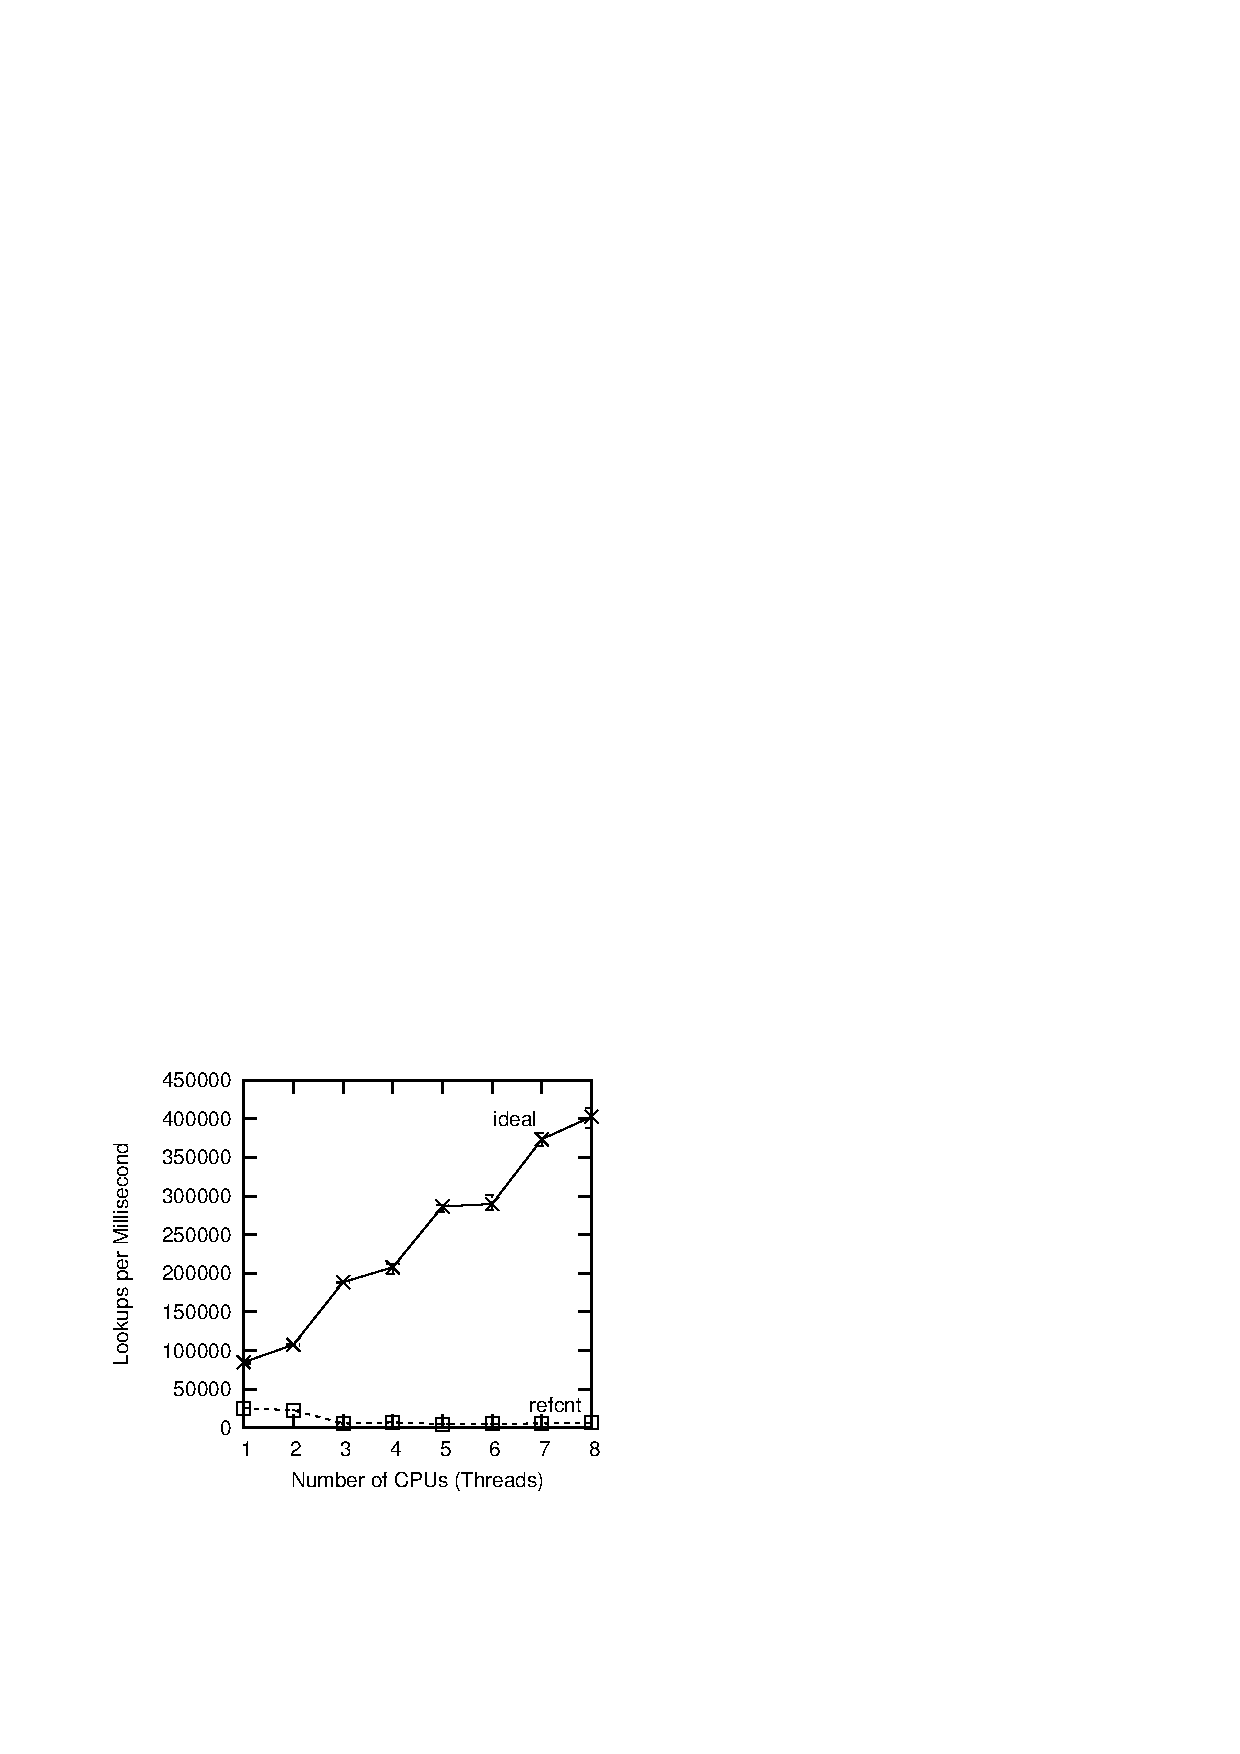
\includegraphics{CodeSamples/defer/data/paulmck.2016/perf-refcnt}}
\caption{Pre-BSD Routing Table Protected by Reference Counting}
\label{fig:defer:Pre-BSD Routing Table Protected by Reference Counting}
\end{figure}

Figure~\ref{fig:defer:Pre-BSD Routing Table Protected by Reference Counting}
shows the performance and scalability of reference counting on a
read-only workload with a ten-element list running on a
single-socket four-core hyperthreaded 2.5GHz x86 system.
The ``ideal'' trace was generated by running the sequential code shown in
Figure~\ref{fig:defer:Sequential Pre-BSD Routing Table}.
The reference-counting performance is abysmal and its scalability even
more so, with the ``refcnt'' trace dropping down onto the x~axis.
This should be no surprise in view of
Chapter~\ref{chp:Hardware and its Habits}:
The reference-count acquisitions and releases have added frequent
shared-memory writes to an otherwise read-only workload, thus
incurring severe retribution from the laws of physics.
As well it should, given that all the wishful thinking in the world
is not going to increase the speed of light or decrease the size of
the atoms used in modern digital electronics.

\QuickQuiz{}
	Why the stairsteps in the ``ideal'' line in
	Figure~\ref{fig:defer:Pre-BSD Routing Table Protected by Reference Counting}?
	Shouldn't it be a straight line?
\QuickQuizAnswer{
	The stair-steps are due to hyperthreading.
	On this particular system, the hardware threads in a given
	core have consecutive CPU numbers.
	In addition, this particular pointer-following
	low-cache-miss-rate workload seems
	to allow a single hardware thread to consume most of the
	relevant resources within its core.
	Workloads featuring heavier computational loads should be
	expected to gain greater benefit from each core's second
	hardware thread.
} \QuickQuizEnd

But it gets worse.

Running multiple updater threads repeatedly invoking
\co{route_add()} and \co{route_del()} will quickly encounter the
\co{abort()} statement on line~37 of
Figure~\ref{fig:defer:Reference-Counted Pre-BSD Routing Table Lookup},
which indicates a use-after-free bug.
This in turn means that the reference counts are not only profoundly
degrading scalability and performance, but also failing to provide
the needed protection.

One sequence of events leading to the use-after-free bug is as follows,
given the list shown in
Figure~\ref{fig:defer:Pre-BSD Packet Routing List}:

\begin{enumerate}
\item	Thread~A looks up address~42, reaching line~33 of
	\co{route_lookup()} in
	Figure~\ref{fig:defer:Reference-Counted Pre-BSD Routing Table Lookup}.
	In other words, Thread~A has a pointer to the first element,
	but has not yet acquired a reference to it.
\item	Thread~B invokes \co{route_del()} in
	Figure~\ref{fig:defer:Reference-Counted Pre-BSD Routing Table Add/Delete}
	to delete the route entry for address~42.
	It completes successfully, and because this entry's \co{->re_refcnt}
	field was equal to the value one, it invokes
	\co{re_free()} to set the \co{->re_freed} field and to free the entry.
\item	Thread~A continues execution of \co{route_lookup()}.
	Its \co{rep} pointer is non-\co{NULL}, but line~36 sees that
	its \co{->re_freed} field is non-zero, so line~37 invokes
	\co{abort()}.
\end{enumerate}

The problem is that the reference count is located in the object
to be protected, but that means that there is no protection during
the instant in time when the reference count itself if being acquired!
This is the reference-counting counterpart of a locking issue noted
by Gamsa et al.~\cite{Gamsa99}.
One could imagine using a global lock or reference count to protect
the per-route-entry reference-count acquisition, but this would
result in severe contention issues.
Although algorithms exist that allow safe reference-count acquisition
in a concurrent environment~\cite{Valois95a}, they are not only extremely
complex and error-prone~\cite{MagedMichael95a}, but also provide
terrible performance and scalability~\cite{ThomasEHart2007a}.

In short, concurrency has most definitely reduced the usefulness
of reference counting!

\QuickQuiz{}
	If concurrency has ``most definitely reduced the usefulness
	of reference counting'', why are there so many reference
	counters in the Linux kernel?
\QuickQuizAnswer{
	That sentence did say ``reduced the usefulness'', not
	``eliminated the usefulness'', now didn't it?

	Please see
	Section~\ref{sec:together:Refurbish Reference Counting},
	which discusses some of the techniques that the Linux kernel
	uses to take advantage of reference counting in a highly
	concurrent environment.
} \QuickQuizEnd

That said, sometimes it is necessary to look at a problem in an
entirely different way in order to successfully solve it.
The next section describes what could be thought of as an
inside-out reference count that provides decent performance
and scalability.

% defer/hazptr.tex
% Can I hazptr cheezeberger?

\section{Hazard Pointers}
\label{sec:defer:Hazard Pointers}

동시적으로 수행되는 레퍼런스 카운팅에서의 문제를 해결하는 한가지 방법은
레퍼런스 카운터들을 뒤집어서 구현하는 것으로,
데이터 원소에 저장되어 있는 정수를 증가시키는 게 아니라, CPU 별 (또는 쓰레드별)
리스트들에 그 데이터 원소로의 포인터를 저장해 두는 것입니다.
이런 리스트의 각 원소들은 \emph{해저드 포인터}~\cite{MagedMichael04a} 라고
불립니다.\footnote{
	그와 독립적으로 다른 사람들에 의해 개발된 것도
	있습니다~\cite{HerlihyLM02}.}
주어진 데이터 원소의 ``가상 레퍼런스 카운터'' 의 값은 그 원소를 레퍼런스 하고
있는 해저드 포인터들의 갯수를 세는 것으로 얻어질 수 있습니다.
따라서, 그 원소가 읽기를 하는 쓰레드들에 의해 접근할 수 없게 된다면, 그리고
더이상 그 원소를 레퍼런스 하고 있는 해저드 포인터가 더이상 존재하지 않는다면,
그 원소는 안전하게 메모리 해제될 수 있습니다.
\iffalse

One way of avoiding problems with concurrent reference counting
is to implement the reference counters
inside out, that is, rather than incrementing an integer stored in the
data element, instead store a pointer to that data element in
per-CPU (or per-thread) lists.
Each element of these lists is called a
\emph{hazard pointer}~\cite{MagedMichael04a}.\footnote{
	Also independently invented by others~\cite{HerlihyLM02}.}
The value of a given data element's ``virtual reference counter'' can
then be obtained by counting the number of hazard pointers referencing
that element.
Therefore, if that element has been rendered inaccessible to readers,
and there are no longer any hazard pointers referencing it, that element
may safely be freed.
\fi

{ \scriptsize
\begin{verbbox}
 1 int hp_store(void **p, void **hp)
 2 {
 3   void *tmp;
 4 
 5   tmp = ACCESS_ONCE(*p);
 6   ACCESS_ONCE(*hp) = tmp;
 7   smp_mb();
 8   if (tmp != ACCESS_ONCE(*p) ||
 9       tmp == HAZPTR_POISON) {
10     ACCESS_ONCE(*hp) = NULL;
11     return 0;
12   }
13   return 1;
14 }
15 
16 void hp_erase(void **hp)
17 {
18   smp_mb();
19   ACCESS_ONCE(*hp) = NULL;
20   hp_free(hp);
21 }
\end{verbbox}
}
\begin{figure}[tbp]
\centering
\theverbbox
\caption{Hazard-Pointer Storage and Erasure}
\label{fig:defer:Hazard-Pointer Storage and Erasure}
\end{figure}

물론, 이 말은 해저드 포인터 획득은 동시의 삭제들에 의한 정리 과정의 경주들을
막기 위해 매우 조심스럽게 행해져야만 합니다.
그런 한가지 구현이
Figure~\ref{fig:defer:Hazard-Pointer Storage and Erasure} 에 보여져 있는데,
line~1-13 에서 \co{hp_store()} 를 보이고 line~15-20 에서 \co{hp_erase()} 를
보이고 있습니다.
\co{smp_mb()} 기능은 Section~\ref{sec:advsync:Memory Barriers} 에서 자세히
설명될 겁니다만, 이 간단한 개략적 설명의 목표를 위해서는 무시되어도 될 겁니다.

\co{hp_store()} 함수는 동시의 수정을 체크하면서 \co{p} 에 의해 레퍼런스되는
포인터가 있는 데이터 원소를 위한 해저드 포인터를 \co{hp} 에 저장합니다.
동시의 수정이 이뤄졌다면, \co{hp_store()} 는 해저드 포인터를 저장하는 것을
거부하고 0을 리턴함으로써 호출자는 다시 처음부터 데이터 접근을 다시 시작해야
함을 알립니다.
그렇지 않다면, \co{hp_store()} 는 해당 데이터 원소를 위한 해저드 포인터를
성공적으로 기록했음을 알리기 위해 1을 리턴합니다.
\iffalse

Of course, this means that hazard-pointer acquisition must be carried
out quite carefully in order to avoid destructive races with concurrent
deletion.
One implementation is shown in
Figure~\ref{fig:defer:Hazard-Pointer Storage and Erasure},
which shows \co{hp_store()} on lines~1-13 and \co{hp_erase()} on
lines~15-20.
The \co{smp_mb()} primitive will be described in detail in
Section~\ref{sec:advsync:Memory Barriers}, but may be ignored for
the purposes of this brief overview.

The \co{hp_store()} function records a hazard pointer at \co{hp} for the data
element whose pointer is referenced by \co{p}, while checking for
concurrent modifications.
If a concurrent modification occurred, \co{hp_store()} refuses to record
a hazard pointer, and returns zero to indicate that the caller must
restart its traversal from the beginning.
Otherwise, \co{hp_store()} returns one to indicate that it successfully
recorded a hazard pointer for the data element.
\fi

\QuickQuiz{}
	Figure~\ref{fig:defer:Hazard-Pointer Storage and Erasure}
	의 \co{hp_store()} 는 왜 데이터 원소로의 접근을 두번이나 간접적으로
	하는거죠?
	왜 \co{void *} 가 아니라 \co{void **} 인 건가요?
	\iffalse

	Why does \co{hp_store()} in
	Figure~\ref{fig:defer:Hazard-Pointer Storage and Erasure}
	take a double indirection to the data element?
	Why not \co{void *} instead of \co{void **}?
	\fi
\QuickQuizAnswer{
	\co{hp_record()} 는 동시의 수정에 대해서 체크를 해봐야 하기 때문입니다.
	이 일을 하기 위해서는 그 원소로의 포인터로의 포인터가 필요한데, 그게
	있으면 해당 원소로의 포인터로의 수정이 있었는지 검사할 수 있기
	때문입니다.
	\iffalse

	Because \co{hp_record()} must check for concurrent modifications.
	To do that job, it needs a pointer to a pointer to the element,
	so that it can check for a modification to the pointer to the
	element.
	\fi
} \QuickQuizEnd

\QuickQuiz{}
	\co{hp_store()} 의 호출자는 실패했을 때 왜 데이터 접근을 처음부터 다시
	시작해야 하는거죠?
	데이터 구조체가 매우 크다면 좀 비효율적이지 않나요?
	\iffalse

	Why does \co{hp_store()}'s caller need to restart its
	traversal from the beginning in case of failure?
	Isn't that inefficient for large data structures?
	\fi
\QuickQuizAnswer{
	어떻게 보면 좀 비효율적일 수도 있겠습니다만 분명한 사실은 정확성을 위해
	그런 처음부터의 재시작이 반드시 필요하다는 점입니다.
	이를 확실히 보기 위해, 원소~A, B, 그리고~C 를 가지고 있는 해저드
	포인터로 보호되는 링크드 리스트가 다음의 일련의 이벤트들을 받는다고
	생각해 봅시다:
	\iffalse

	It might be inefficient in some sense, but the fact is that
	such restarting is absolutely required for correctness.
	To see this, consider a hazard-pointer-protected linked list
	containing elements~A, B, and~C that is subjecte to the
	following sequence of events:
	\fi

	\begin{enumerate}
	\item	쓰레드~0 가 원소~B 로의 해저드 포인터를 저장합니다
		(아마도 원소~A 를 거쳐 원소~B 를 찾아왔을 겁니다).
	\item	쓰레드~1 이 리스트로부터 원소~B 를 삭제하는데, 이를 위해 원소~B
		에서 원소~C 로의 포인터를 이 삭제 작업을 표시하기 위해 특수한
		\co{HAZPTR_POISON} 값으로 설정합니다.
		Thread~0 는 원소~B 로의 해저드 포인터를 가지고 있으므로, 아직
		정리될 수 없습니다.
	\item	쓰레드~1 이 리스트에서 원소~C 를 삭제합니다.
		원소~C 를 레퍼런스 하는 해저드 포인터들이 존재하지 않으므로,
		원소~C 는 곧바로 메모리 해제될 수 있습니다.
	\item	쓰레드~0 이 이제 없어진 원소~B 의 다음 원소로의 해저드 포인터를
		얻으려 합니다만, \co{HAZPTR_POISON} 값을 보게 되고, 따라서 0을
		리턴해서, 호출자가 리스트의 시작점부터 탐색을 다시 시작하도록
		강제합니다.
	\iffalse

	\item	Thread~0 stores a hazard pointer to element~B
		(having presumably traversed to element~B from element~A).
	\item	Thread~1 removes element~B from the list, which sets
		the pointer from element~B to element~C to a special
		\co{HAZPTR_POISON} value in order to mark the deletion.
		Because Thread~0 has a hazard pointer to element~B,
		it cannot yet be freed.
	\item	Thread~1 removes element~C from the list.
		Because there are no hazard pointers referencing element~C,
		it is immediately freed.
	\item	Thread~0 attempts to acquire a hazard pointer to
		now-removed element~B's successor, but sees the
		\co{HAZPTR_POISON} value, and thus returns zero,
		forcing the caller to restart its traversal from the
		beginning of the list.
	\fi
	\end{enumerate}

	따라서 처음부터 다시 탐색하는게 좋은 방법인데, 이렇게 하지 않는다면
	쓰레드~0 는 이제는 제거된 원소~C 에 액세스를 시도할 수 있는데, 이는
	임의의 끔찍한 메모리 오염을 일으키는 결과를 만들어낼 수 있는데, 특히나
	원소~C 를 위해 사용되던 메모리가 어떤 다른 목적으로 재할당 되었다면
	특히 그럴 것이기 때문입니다.

	그와는 별개로, 해저드 포인터의 재시작은 최소한의 메모리 사용량을 유지할
	수 있도록 함을 이해하기 바랍니다.
	현재 해저드 포인터로 레퍼런스 되고 있지 않은 오브젝트는 곧바로 해제될
	수 있습니다.
	대조적으로,
	Section~\ref{sec:defer:Read-Copy Update (RCU)} 에서는 read-side
	재시도를 방지하지만 (read-side 오버헤드도 최소화 시킵니다), 훨씬 큰
	메모리 사용량을 갖는 메커니즘을 이야기할 겁니다.
	\iffalse

	Which is a very good thing, because otherwise Thread~0 would
	have attempted to access the now-freed element~C,
	which might have resulted in arbitrarily horrible
	memory corruption, especially if the memory for
	element~C had since been re-allocated for some other
	purpose.

	All that aside, please understand that hazard pointers's
	restarting allows it to maintain a minimal memory footprint.
	Any object not currently referenced by some hazard pointer
	may be immediately freed.
	In contrast,
	Section~\ref{sec:defer:Read-Copy Update (RCU)}
	will discuss a mechanism that avoids read-side retries
	(and minimizes read-side overhead), but has a much larger
	memory footprint.
	\fi
} \QuickQuizEnd

\QuickQuiz{}
	해저드 포인터들에 대한 논문들은 각각의 포인터의 아래 비트들을 지워진
	원소들을 마크하기 위해 사용한다고 하는데, \co{HAZPTR_POISON} 은 뭔가요?
	\iffalse

	Given that papers on hazard pointers use the bottom bits
	of each pointer to mark deleted elements, what is up with
	\co{HAZPTR_POISON}?
	\fi
\QuickQuizAnswer{
	출간된 논문의 해저드 포인터 구현들은 그 삽입과 삭제를 위해 non-blocking
	동기화 기법들을 사용했습니다.
	이런 기법들은 데이터 구조체를 가로지르며 읽기를 하는 쓰레드들이
	업데이트를 하는 쓰레드들이 그들의 업데이트를 완료하도록 ``도움''을 줄
	것을 필요로 하는데, 이 말은 읽기를 하는 쓰레드들은 삭제된 원소의 다음
	원소를 봐야만 한다는 뜻입니다.

	반면에, 우리는 업데이트 작업들을 동기화 시키는데 락킹을 사용할 것인데,
	이렇게 되면 읽기를 하는 쓰레드들이 업데이트를 하는 쓰레드들이 그들의
	업데이트를 완료할 수 있도록 돕는 일을 해줄 필요가 없어져서 포인터들의
	아래쪽 비트들을 놔둘 수 있게 해줍니다.
	이 방법은 읽기를 하는쪽 코드를 좀 더 간단하고 빠르게 해줍니다.
	\iffalse

	The published implementations of hazard pointers used
	non-blocking synchronization techniques for insertion
	and deletion.
	These techniques require that readers traversing the
	data structure ``help'' updaters complete their updates,
	which in turn means that readers need to look at the successor
	of a deleted element.

	In contrast, we will be using locking to synchronize updates,
	which does away with the need for readers to help updaters
	complete their updates, which in turn allows us to leave
	pointers' bottom bits alone.
	This approach allows read-side code to be simpler and faster.
	\fi
} \QuickQuizEnd

해저드 포인터들을 사용하는 알고리즘들은 데이터 구조체를 지나가는 중 어떤
단계에서든 재시작할 수 있으므로, 그런 알고리즘들은 모든 필요한 해저드
포인터들을 얻어오는 작업이 끝나기 전까지는 이 데이터 구조체에 어떤 변경을
가하지 않도록 특별한 주의를 반드시 기울여야만 합니다.
\iffalse

Because algorithms using hazard pointers might be restarted at any
step of their traversal through the data structure, such algorithms
must typically take care to avoid making any changes to the data
structure until after they have acquired all relevant hazard pointers.
\fi

\QuickQuiz{}
	하지만 해저드 포인터들에 있는 이런 제약사항들은 다른 형태의 레퍼런스
	카운팅에도 똑같이 적용되는 거 아닌가요?
	\iffalse

	But don't these restrictions on hazard pointers also apply
	to other forms of reference counting?
	\fi
\QuickQuizAnswer{
	이런 제약사항은 레퍼런스 획득이 실패할 수 있는 레퍼런스 카운팅
	메커니즘들에만 적용됩니다.
	\iffalse

	These restrictions apply only to reference-counting mechanisms whose
	reference acquisition can fail.
	\fi
} \QuickQuizEnd

이런 제약사항들은 읽기를 하는 쓰레드들에는 커다란 이득으로 귀결되는데, 해저드
포인터들은 각 CPU/쓰레드에 지역적으로 저장되기 때문으로, 이에 의해 데이터
구조체들을 횡단하는 작업은 완전히 읽기만 하면서 행해질 수 있다는 사실 덕입니다.
page~\pageref{fig:count:Optimization and the Four Parallel-Programming Tasks}
의
Figure~\ref{fig:count:Optimization and the Four Parallel-Programming Tasks}
를 다시 인용하자면, 해저드 포인터들은 CPU 캐시들이 리소스 복사를 할 수 있게
해서 병렬 액세스 컨트롤 메커니즘을 약화시키는 걸 가능하게 하고, 따라서 성능과
확장성을 높여줍니다.
다른 메커니즘들과의 성능 비교는 Chapter~\ref{chp:Data Structures} 와 다른
출간물들~\cite{ThomasEHart2007a,McKenney:2013:SDS:2483852.2483867,MagedMichael04a}
에서 얻을 수 있을 겁니다.

해저드 포인터들은 레퍼런스 카운터들보다 훨씬 더 확장성 있습니다만 여전히 읽기를
하는 쓰레드들이 공유 메모리에 쓰기를 하게 합니다.
다음 섹션의 주제인 시퀀스 카운터들은 읽기 쪽의 쓰기를 완전히 막습니다.
\iffalse

These restrictions result in great benefits to readers, courtesy of the
fact that the hazard pointers are stored local to each CPU/thread,
which in turn allows traversals of the data structures themselves to
be carried out in a completely read-only fashion.
Referring back to
Figure~\ref{fig:count:Optimization and the Four Parallel-Programming Tasks}
on
page~\pageref{fig:count:Optimization and the Four Parallel-Programming Tasks},
hazard pointers enable the CPU caches to do resource replication, which
in turn allows weakening of the parallel-access-control mechanism,
thus boosting performance and scalability.
Performance comparisons with other mechanisms may be found in
Chapter~\ref{chp:Data Structures}
and in other publications~\cite{ThomasEHart2007a,McKenney:2013:SDS:2483852.2483867,MagedMichael04a}.
\fi

{ \scriptsize
\begin{verbbox}
 1 struct route_entry {
 2   struct hazptr_head hh;
 3   struct route_entry *re_next;
 4   unsigned long addr;
 5   unsigned long iface;
 6   int re_freed;
 7 };
 8 struct route_entry route_list;
 9 DEFINE_SPINLOCK(routelock);
10 hazard_pointer __thread *my_hazptr;
11
12 unsigned long route_lookup(unsigned long addr)
13 {
14   int offset = 0;
15   struct route_entry *rep;
16   struct route_entry **repp;
17
18 retry:
19   repp = &route_list.re_next;
20   do {
21     rep = ACCESS_ONCE(*repp);
22     if (rep == NULL)
23       return ULONG_MAX;
24     if (rep == (struct route_entry *)HAZPTR_POISON)
25       goto retry;
26     my_hazptr[offset].p = &rep->hh;
27     offset = !offset;
28     smp_mb();
29     if (ACCESS_ONCE(*repp) != rep)
30       goto retry;
31     repp = &rep->re_next;
32   } while (rep->addr != addr);
33   if (ACCESS_ONCE(rep->re_freed))
34     abort();
35   return rep->iface;
36 }
\end{verbbox}
}
\begin{figure}[bp]
\centering
\theverbbox
\caption{Hazard-Pointer Pre-BSD Routing Table Lookup}
\label{fig:defer:Hazard-Pointer Pre-BSD Routing Table Lookup}
\end{figure}

{ \scriptsize
\begin{verbbox}
 1 int route_add(unsigned long addr,
 2               unsigned long interface)
 3 {
 4   struct route_entry *rep;
 5
 6   rep = malloc(sizeof(*rep));
 7   if (!rep)
 8     return -ENOMEM;
 9   rep->addr = addr;
10   rep->iface = interface;
11   rep->re_freed = 0;
12   spin_lock(&routelock);
13   rep->re_next = route_list.re_next;
14   route_list.re_next = rep;
15   spin_unlock(&routelock);
16   return 0;
17 }
18
19 int route_del(unsigned long addr)
20 {
21   struct route_entry *rep;
22   struct route_entry **repp;
23
24   spin_lock(&routelock);
25   repp = &route_list.re_next;
26   for (;;) {
27     rep = *repp;
28     if (rep == NULL)
29       break;
30     if (rep->addr == addr) {
31       *repp = rep->re_next;
32       rep->re_next =
33           (struct route_entry *)HAZPTR_POISON;
34       spin_unlock(&routelock);
35       hazptr_free_later(&rep->hh);
36       return 0;
37     }
38     repp = &rep->re_next;
39   }
40   spin_unlock(&routelock);
41   return -ENOENT;
42 }
\end{verbbox}
}
\begin{figure}[bp]
\centering
\theverbbox
\caption{Hazard-Pointer Pre-BSD Routing Table Add/Delete}
\label{fig:defer:Hazard-Pointer Pre-BSD Routing Table Add/Delete}
\end{figure}

The Pre-BSD routing example can use hazard pointers as shown in
Figure~\ref{fig:defer:Hazard-Pointer Pre-BSD Routing Table Lookup}
for data structures and \co{route_lookup()}, and in
Figure~\ref{fig:defer:Hazard-Pointer Pre-BSD Routing Table Add/Delete}
for \co{route_add()} and \co{route_del()}
(\path{route_hazptr.c}).
As with reference counting, the hazard-pointers implementation
is quite similar to the sequential algorithm shown in
Figure~\ref{fig:defer:Sequential Pre-BSD Routing Table}
on
page~\pageref{fig:defer:Sequential Pre-BSD Routing Table},
so only differences will be discussed.

Starting with
Figure~\ref{fig:defer:Hazard-Pointer Pre-BSD Routing Table Lookup},
line~2 shows the \co{->hh} field used to queue objects pending
hazard-pointer free,
line~6 shows the \co{->re_freed} field used to detect use-after-free bugs,
and lines~24-30 attempt to acquire a hazard pointer, branching
to line~18's \co{retry} label on failure.

In
Figure~\ref{fig:defer:Hazard-Pointer Pre-BSD Routing Table Add/Delete},
line~11 initializes \co{->re_freed},
lines~32 and~33 poison the \co{->re_next} field of the newly removed
object, and
line~35 passes that object to the hazard pointers's
\co{hazptr_free_later()} function, which will free that object once it
is safe to do so.
The spinlocks work the same as in
Figure~\ref{fig:defer:Reference-Counted Pre-BSD Routing Table Add/Delete}.

\begin{figure}[tb]
\centering
\resizebox{2.5in}{!}{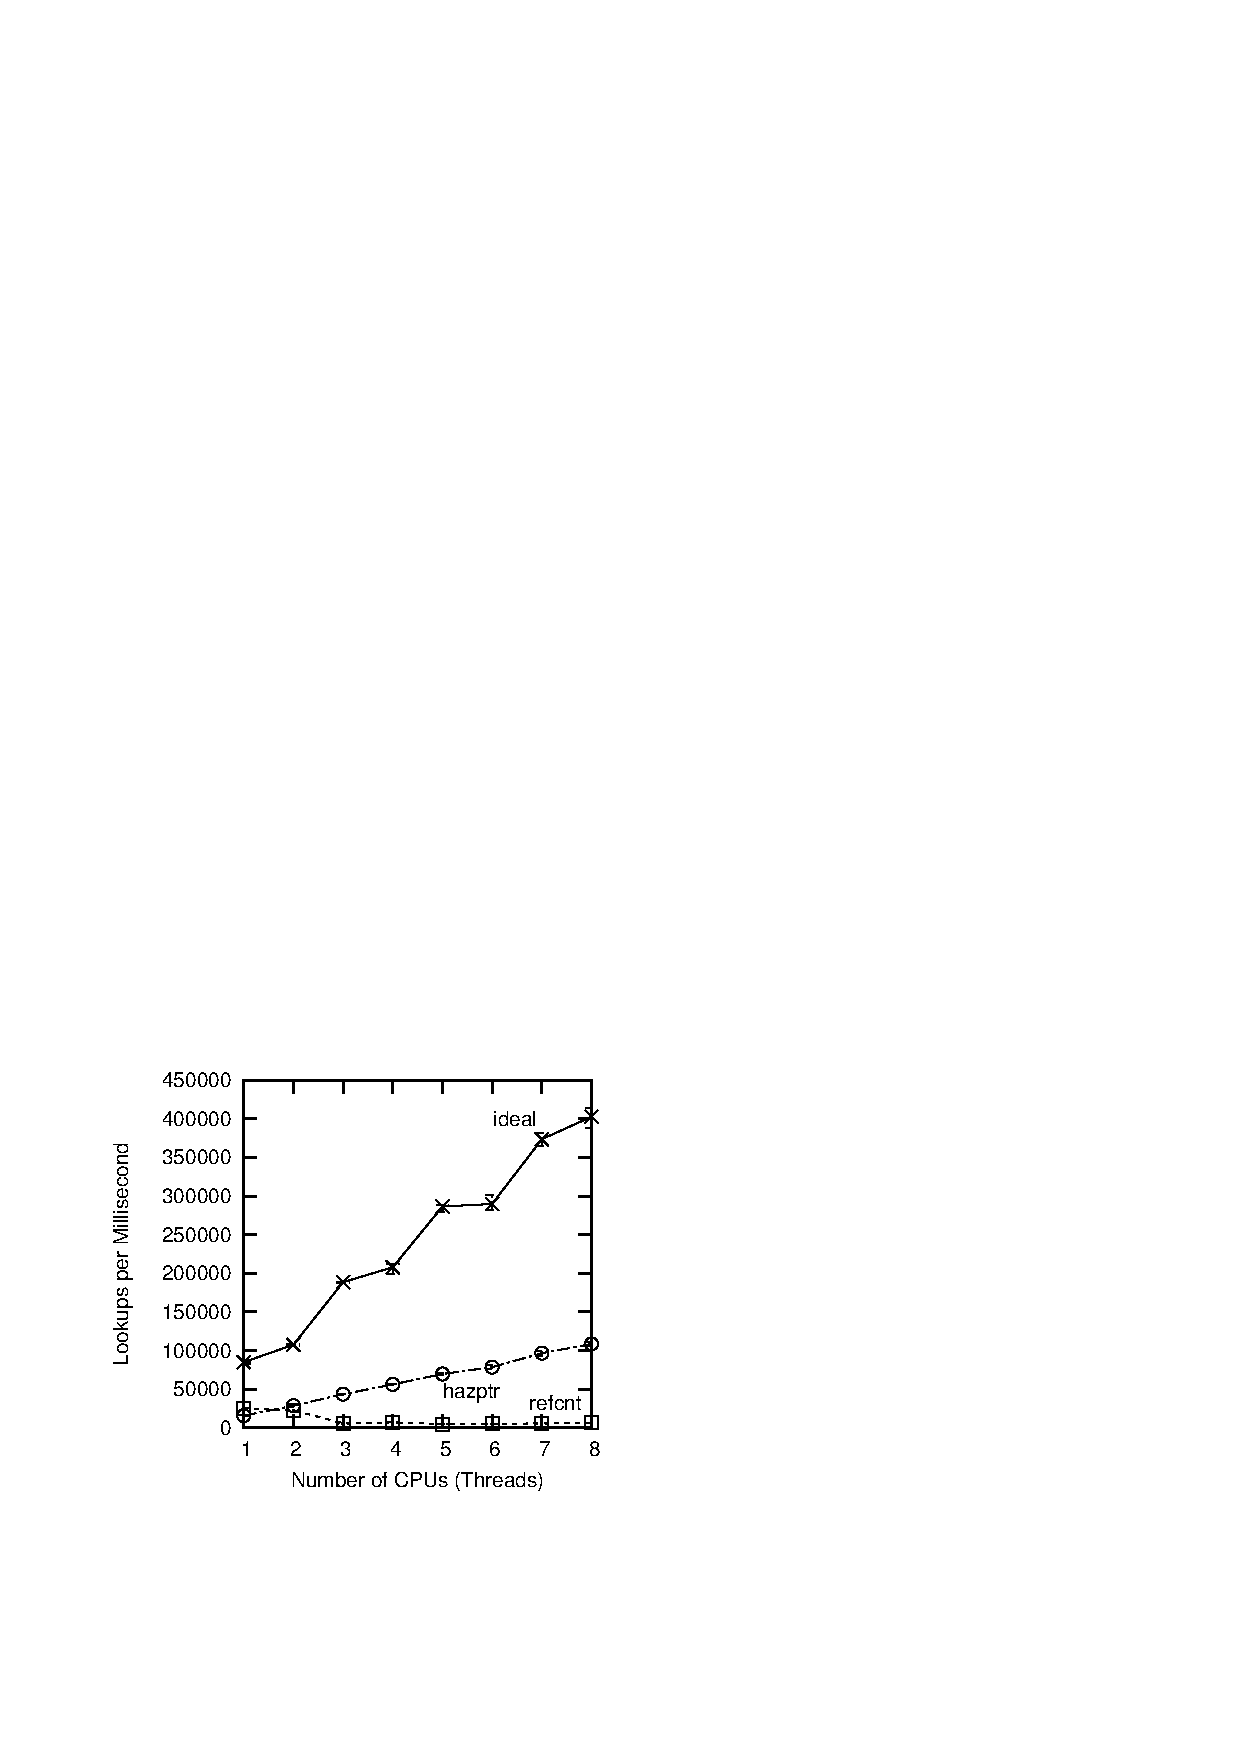
\includegraphics{CodeSamples/defer/data/paulmck.2016/perf-hazptr}}
\caption{Pre-BSD Routing Table Protected by Hazard Pointers}
\label{fig:defer:Pre-BSD Routing Table Protected by Hazard Pointers}
\end{figure}

Figure~\ref{fig:defer:Pre-BSD Routing Table Protected by Hazard Pointers}
shows the hazard-pointers-protected Pre-BSD routing algorithm's
performance on the same read-only workload as for
Figure~\ref{fig:defer:Pre-BSD Routing Table Protected by Reference Counting}.
Although hazard pointers scales much better than does reference counting,
hazard pointers still require readers to do writes to shared
memory (albeit with much improved locality of reference),
and also require a full memory barrier and retry check for each
object traversed.
Therefore, hazard pointers's performance is far short of ideal.
On the other hand, hazard pointers do operate correctly for workloads
involving concurrent updates.

\QuickQuiz{}
	The paper ``Structured Deferral: Synchronization via
	Procrastination''~\cite{McKenney:2013:SDS:2483852.2483867}
	shows that hazard pointers have near-ideal performance.
	Whatever happened in
	Figure~\ref{fig:defer:Pre-BSD Routing Table Protected by Hazard Pointers}???
\QuickQuizAnswer{
	First,
	Figure~\ref{fig:defer:Pre-BSD Routing Table Protected by Hazard Pointers}
	has a linear y-axis, while most of the graphs in the
	``Structured Deferral'' paper have logscale y-axes.
	Next, that paper uses hash tables, while
	Figure~\ref{fig:defer:Pre-BSD Routing Table Protected by Hazard Pointers}'s
	uses a simple linked list.
	Finally, that paper used a larger and older x86 system, while
	a newer but smaller system that was used to generate the data
	shown in
	Figure~\ref{fig:defer:Pre-BSD Routing Table Protected by Hazard Pointers}.
} \QuickQuizEnd

The next section attempts to improve on hazard pointers by using
sequence locks, which avoid both read-side writes and per-object memory
barriers.

% defer/seqlock.tex
% mainfile: ../perfbook.tex
% SPDX-License-Identifier: CC-BY-SA-3.0

\section{Sequence Locks}
\label{sec:defer:Sequence Locks}
%
\epigraph{It'll be just like starting over.}{\emph{John Lennon}}

출간된 시퀀스 락 기록은~\cite{10.1145/800212.806505,10.1145/359863.359878}
reader-writer 락킹의 그것만큼이나 오래 되었습니다만, 시퀀스 락은 상대적으로 덜
알려져 있습니다.
시퀀스 락은 리눅스 커널에서 읽기 쓰레드에게 일관적인 상태로 보여야만 하는
읽기가 대부분인 데이터를 위해 사용됩니다.
하지만, reader-writer 락킹과 달리, 읽기 쓰레드는 쓰기 쓰레드를 배제시키지
않습니다.
그 대신, 해저드 포인터처럼, 시퀀스 락은 읽기 쓰레드가 동시의 쓰기
쓰레드로부터의 활동을 탐지한 경우 오퍼레이션을 \emph{재시도} 하게 합니다.
Figure~\ref{fig:defer:Reader And Uncooperative Sequence Lock}
에서 볼 수 있듯, 읽기 쓰레드들이 아주 가끔만 재시도를 해야 하게끔 코드를
설계하는게 중요합니다.

\iffalse

The published sequence-lock
record~\cite{10.1145/800212.806505,10.1145/359863.359878}
extends back as far as that of reader-writer locking, but sequence locks
nevertheless remain in relative obscurity.
Sequence locks are used in the Linux kernel for read-mostly data that
must be seen in a consistent state by readers.
However, unlike reader-writer locking, readers do not exclude writers.
Instead, like hazard pointers, sequence locks force readers to
\emph{retry} an operation if they detect activity from a concurrent writer.
As can be seen from
Figure~\ref{fig:defer:Reader And Uncooperative Sequence Lock},
it is important to design code using sequence locks so that readers
very rarely need to retry.

\fi

\begin{figure}[tb]
\centering
\resizebox{3in}{!}{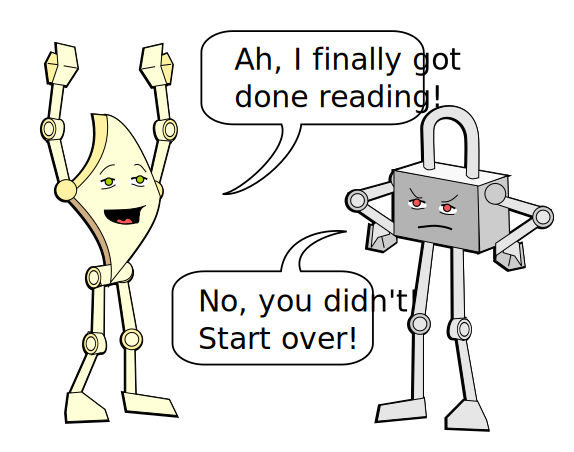
\includegraphics{cartoons/r-2014-Start-over}}
\caption{Reader And Uncooperative Sequence Lock}
\label{fig:defer:Reader And Uncooperative Sequence Lock}
\end{figure}

\QuickQuiz{
	이 시퀀스 락 이야기는 왜 Chapter~\ref{chp:Locking} 에 있지 않죠, 이건
	\emph{락킹} 이잖아요?

	\iffalse

	Why isn't this sequence-lock discussion in Chapter~\ref{chp:Locking},
	you know, the one on \emph{locking}?

	\fi

}\QuickQuizAnswer{
	이 시퀀스 락 메커니즘은 실제로 두개의 별개의 동기화 메커니즘인 시퀀스
	카운트와 락킹의 조합입니다.
	사실, 이 시퀀스 카운트 메커니즘은 리눅스 커널에서
	\co{write_seqcount_begin()} 과 \co{write_seqcount_end()} 기능을 통해
	사용할 수 있습니다.

	하지만, \co{write_seqlock()} 과 \co{write_sequnlock()} 의 조합이 리눅스
	커널에서는 훨씬 더 많이 사용됩니다.
	더 중요하게, 많은 사람들이 ``시퀀스 카운트'' 보다는 ``시퀀스 락''
	이라고 말할 때 더 잘 알아들을 겁니다.

	따라서 이 섹션은 사람들이 제목으로부터 이게 무엇인지 이해할 수 있게끔
	``Sequence Locks'' 라고 제목지어져 있으며, ``Deferred Processing'' 으로
	표현되어 있는 이유는 (1) ``시퀀스 락'' 의 ``시퀀스 카운트'' 를 강조하고
	(2) ``시퀀스 락'' 은 간단한 락 그 이상의 무엇이기 때문입니다.

	\iffalse

	The sequence-lock mechanism is really a combination of two
	separate synchronization mechanisms, sequence counts and
	locking.
	In fact, the sequence-count mechanism is available separately
	in the Linux kernel via the
	\co{write_seqcount_begin()} and \co{write_seqcount_end()}
	primitives.

	However, the combined \co{write_seqlock()} and
	\co{write_sequnlock()} primitives are used much more heavily
	in the Linux kernel.
	More importantly, many more people will understand what you
	mean if you say ``sequence lock'' than if you say
	``sequence count''.

	So this section is entitled ``Sequence Locks'' so that people
	will understand what it is about just from the title, and
	it appears in the ``Deferred Processing'' because (1) of the
	emphasis on the ``sequence count'' aspect of ``sequence locks''
	and (2) because a ``sequence lock'' is much more than merely
	a lock.

	\fi

}\QuickQuizEnd

\begin{listing}[bp]
\begin{VerbatimL}
do {
	seq = read_seqbegin(&test_seqlock);
	/* read-side access. */
} while (read_seqretry(&test_seqlock, seq));
\end{VerbatimL}
\caption{Sequence-Locking Reader}
\label{lst:defer:Sequence-Locking Reader}
\end{listing}

\begin{listing}[bp]
\begin{VerbatimL}
write_seqlock(&test_seqlock);
/* Update */
write_sequnlock(&test_seqlock);
\end{VerbatimL}
\caption{Sequence-Locking Writer}
\label{lst:defer:Sequence-Locking Writer}
\end{listing}

시퀀스 락킹의 핵심 컴포넌트는 시퀀스 숫자로, 업데이트 쓰레드가 없을 때에는
짝수가 되며 진행중인 업데이트가 있을 때에는 홀수가 됩니다.
그럼 읽기 쓰레드는 각 액세스 전과 후에 값을 스냅샷 찍어둘 수 있습니다.
두개의 스냅샷 중 어느 하나라도 홀수를 가지고 있다면, 또는 이 두 스냅샷이
다르다면, 동시의 업데이트가 있었다는 말이 되며, 읽기 쓰레드는 이 액세스의
결과를 폐기하고 재시도 해야 합니다.
따라서 읽기 쓰레드는 시퀀스 락으로 보호되는 데이터에 접근할 때
Listing~\ref{lst:defer:Sequence-Locking Reader} 에 보인 \co{read_seqbegin()} 과
\co{read_seqretry()} 함수를 사용해야 합니다.
스기 쓰레드는 각 업데이트 전과 후에 이 값을 증가시켜야만 하고 한번에 하나의
쓰기 쓰레드만이 허용됩니다.
따라서 쓰기 스레드는 시퀀스 락으로 보호되는 데이터를 업데이트 할 때
Listing~\ref{lst:defer:Sequence-Locking Writer} 에 보인 \co{write_seqlock()} 과
\co{write_sequnlock()} 을 사용해야 합니다.

그 결과, 시퀀스 락으로 보호되는 데이터는 임의의 큰 수의 동시 읽기 쓰레드를 가질
수 있지만, 한번에 하나의 쓰기 쓰레드만 가질 수 있습니다.
시퀀스 락킹은 리눅스 커널에서 시간 계측에서 측정 정도를 보호하기 위해
사용됩니다.
시퀀스 락킹은 또한 경로명 순회 중 동시의 이름 변경 오퍼레이션을 감지하기 위해
사용됩니다.

\iffalse

The key component of sequence locking is the sequence number, which has
an even value in the absence of updaters and an odd value if there
is an update in progress.
Readers can then snapshot the value before and after each access.
If either snapshot has an odd value, or if the two snapshots differ,
there has been a concurrent update, and the reader must discard
the results of the access and then retry it.
Readers therefore use the \co{read_seqbegin()} and \co{read_seqretry()}
functions shown in Listing~\ref{lst:defer:Sequence-Locking Reader}
when accessing data protected by a sequence lock.
Writers must increment the value before and after each update,
and only one writer is permitted at a given time.
Writers therefore use the \co{write_seqlock()} and \co{write_sequnlock()}
functions shown in Listing~\ref{lst:defer:Sequence-Locking Writer}
when updating data protected by a sequence lock.

As a result, sequence-lock-protected data can have an arbitrarily
large number of concurrent readers, but only one writer at a time.
Sequence locking is used in the Linux kernel to protect calibration
quantities used for timekeeping.
It is also used in pathname traversal to detect concurrent rename operations.

\fi

\begin{listing}[tb]
\input{CodeSamples/defer/seqlock@impl.fcv}
\caption{Sequence-Locking Implementation}
\label{lst:defer:Sequence-Locking Implementation}
\end{listing}

시퀀스 락의 간단한 구현이
Listing~\ref{lst:defer:Sequence-Locking Implementation}
(\path{seqlock.h}) 에 보여 있습니다.
\begin{fcvref}[ln:defer:seqlock:impl:typedef]
\co{seqlock_t} 데이터 구조는 \clnrefrange{b}{e} 에 보여져 있는데 시퀀스 숫자와
함께 쓰기 쓰레드들을 순서짓기 위한 락을 포함하고 있습니다.
\end{fcvref}
\begin{fcvref}[ln:defer:seqlock:impl:init]
\Clnrefrange{b}{e} 는 이름이 의미하듯 \co{seqlock_t} 를 초기화 하는
\co{seqlock_init()} 를 보입니다.
\end{fcvref}

\begin{fcvref}[ln:defer:seqlock:impl:read_seqbegin]
\Clnrefrange{b}{e} 는 시퀀스 락 읽기 쪽 크리티컬 섹션을 시작하는
\co{read_seqbegin()} 을 보입니다.
라인~\lnref{fetch} 는 시퀀스 카운터의 스냅샷을 취하고, 라인~\lnref{mb} 는 이
호출자의 크리티컬 섹션이 시작되기 전으로 이 스냅샷 오퍼레이션이 순서지어지도록
합니다.
마지막으로, 라인~\lnref{ret} 는 이 스냅샷의 값을 (least-significant bit 이
지워진채로) 리턴하는데, 호출자는 이를 나중의 \co{read_seqretry()} 호출 시에
넘길 겁니다.
\end{fcvref}

\iffalse

A simple implementation of sequence locks is shown in
Listing~\ref{lst:defer:Sequence-Locking Implementation}
(\path{seqlock.h}).
\begin{fcvref}[ln:defer:seqlock:impl:typedef]
The \co{seqlock_t} data structure is shown on
\clnrefrange{b}{e}, and contains
the sequence number along with a lock to serialize writers.
\end{fcvref}
\begin{fcvref}[ln:defer:seqlock:impl:init]
\Clnrefrange{b}{e} show \co{seqlock_init()}, which, as the name indicates,
initializes a \co{seqlock_t}.
\end{fcvref}

\begin{fcvref}[ln:defer:seqlock:impl:read_seqbegin]
\Clnrefrange{b}{e} show \co{read_seqbegin()}, which begins a sequence-lock
read-side critical section.
Line~\lnref{fetch} takes a snapshot of the sequence counter, and
line~\lnref{mb} orders
this snapshot operation before the caller's critical section.
Finally, line~\lnref{ret} returns the value of the snapshot (with the least-significant
bit cleared), which the caller
will pass to a later call to \co{read_seqretry()}.
\end{fcvref}

\fi

\QuickQuiz{
	Listing~\ref{lst:defer:Sequence-Locking Implementation}
	의 \co{read_seqbegin()} 은 왜 이미 망한 읽기가 시작되게 하는 대신
	아래쪽 bit 이 셋 되었는지 검사하고 내부적으로 재시도 하지 않나요?

	\iffalse

	Why not have \co{read_seqbegin()} in
	Listing~\ref{lst:defer:Sequence-Locking Implementation}
	check for the low-order bit being set, and retry
	internally, rather than allowing a doomed read to start?

	\fi

}\QuickQuizAnswer{
	그건 합법적인 구현이 될 겁니다.
	하지만, 워크로드가 읽기가 대부분이라면, 일반적인 경우 성공적 읽기의
	오버헤드를 증가시킬 수 있는데, 이는 생산적이지 못할 겁니다.
	그러나, 충분히 큰 업데이트 쓰레드의 비율과 충분히 높은 읽기 쓰레드의
	오버헤드가 주어진다면, \co{read_seqbegin()} 내부의 체크를 갖는 것이
	선호될 수 있습니다.

	\iffalse

	That would be a legitimate implementation.
	However, if the workload is read-mostly, it would likely
	increase the overhead of the common-case successful read,
	which could be counter-productive.
	However, given a sufficiently large fraction of updates
	and sufficiently high-overhead readers, having the
	check internal to \co{read_seqbegin()} might be preferable.

	\fi

}\QuickQuizEnd

\begin{fcvref}[ln:defer:seqlock:impl:read_seqretry]
\Clnrefrange{b}{e} 는 연관된 \co{read_seqbegin()} 호출 이후 최소 하나의 쓰기
쓰레드가 존재했다면 true 를 리턴하는 \co{read_seqretry()} 를 보입니다.
라인~\lnref{mb} 는 이 호출자의 라인~\lnref{fetch} 의 시퀀스 카운터의 새
스냅샷을 읽어오기 전의 크리티컬 섹션을 순서짓습니다.
라인~\lnref{ret} 는 이 시퀀스 카운터가 변화되었는지 검사하는데, 달리 말하면
최소 하나의 쓰기 쓰레드가 있었는지 검사하고, 그렇다면 true 를 리턴합니다.
\end{fcvref}

\iffalse

\begin{fcvref}[ln:defer:seqlock:impl:read_seqretry]
\Clnrefrange{b}{e} show \co{read_seqretry()}, which returns true if there
was at least one writer since the time of the corresponding
call to \co{read_seqbegin()}.
Line~\lnref{mb} orders the caller's prior critical section before line~\lnref{fetch}'s
fetch of the new snapshot of the sequence counter.
Line~\lnref{ret} checks whether the sequence counter has changed,
in other words, whether there has been at least one writer, and returns
true if so.
\end{fcvref}

\fi

\QuickQuizSeries{%
\QuickQuizB{
	Listing~\ref{lst:defer:Sequence-Locking Implementation} 의
	line~\ref{ln:defer:seqlock:impl:read_seqretry:mb}
	의 \co{smp_mb()} 는 왜 필요한가요?

	\iffalse

	Why is the \co{smp_mb()} on
	line~\ref{ln:defer:seqlock:impl:read_seqretry:mb} of
	Listing~\ref{lst:defer:Sequence-Locking Implementation}
	needed?

	\fi

}\QuickQuizAnswerB{
	그게 없다면, 컴파일러도 CPU 도 \co{read_seqretry()} 앞의 크리티컬
	섹션을 이 함수 다음으로 재배치 할 권리를 갖습니다.
	이는 이 시퀀스 락이 크리티컬 섹션을 보호하는 걸 방해할 겁니다.
	\co{smp_mb()} 기능은 그런 재배치를 막습니다.

	\iffalse

	If it was omitted, both the compiler and the CPU would be
	within their rights to move the critical section preceding
	the call to \co{read_seqretry()} down below this function.
	This would prevent the sequence lock from protecting the
	critical section.
	The \co{smp_mb()} primitive prevents such reordering.

	\fi

}\QuickQuizEndB
%
\QuickQuizM{
	Listing~\ref{lst:defer:Sequence-Locking Implementation}
	의 코드에서는 더 완화된 형태의 메모리 배리어를 사용할 순 없나요?

	\iffalse

	Can't weaker memory barriers be used in the code in
	Listing~\ref{lst:defer:Sequence-Locking Implementation}?

	\fi

}\QuickQuizAnswerM{
	오래전 버전의 리눅스 커널에서는 안됩니다.

	\begin{fcvref}[ln:defer:seqlock:impl]
	매우 최신 버전의 리눅스 커널에서는
	line~\lnref{read_seqbegin:fetch} 은 \co{READ_ONCE()} 대신
	라인~\lnref{read_seqbegin:mb} 의 \co{smp_mb()} 를 없애도 되게 할 수
	있는 \co{smp_load_acquire()} 를 사용할 수도 있습니다.
	비슷하게, 라인~\lnref{write_sequnlock:inc} 는 예를 들면 다음과 같이
	\co{smp_store_release()} 를 사용할 수 있습니다:

	\iffalse

	In older versions of the Linux kernel, no.

	\begin{fcvref}[ln:defer:seqlock:impl]
	In very new versions of the Linux kernel,
        line~\lnref{read_seqbegin:fetch} could use
	\co{smp_load_acquire()} instead of \co{READ_ONCE()}, which
	in turn would allow the \co{smp_mb()} on
        line~\lnref{read_seqbegin:mb} to be dropped.
	Similarly, line~\lnref{write_sequnlock:inc} could use an
        \co{smp_store_release()}, for
	example, as follows:

	\fi

\begin{VerbatimU}
smp_store_release(&slp->seq, READ_ONCE(slp->seq) + 1);
\end{VerbatimU}

	이는 라인~\lnref{write_sequnlock:mb} 의 \co{smp_mb()} 를 제거할 수 있게
	할 겁니다.
	\end{fcvref}

	\iffalse

	This would allow the \co{smp_mb()} on
	line~\lnref{write_sequnlock:mb} to be dropped.
	\end{fcvref}

	\fi

}\QuickQuizEndM
%
\QuickQuizE{
	시퀀스 락킹 업데이트 쓰레드가 읽기 쓰레드를 starve 시키는 걸 무엇이
	방지하나요?

	\iffalse

	What prevents sequence-locking updaters from starving readers?

	\fi

}\QuickQuizAnswerE{
	아무것도요.
	이것은 시퀀스 락킹의 약점 중 하나이며, 그 결과, 여러분은 시퀀스 락킹을
	읽기가 대부분인 환경에서만 사용해야 합니다.
	그렇지 않다면 읽기 쪽의 starvation 은 여러분의 환경에서는 허용되는
	것이니, 이 경우라면, 시퀀스 락킹 업데이트를 가지고 잘 놀아보시기
	바랍니다!

	\iffalse

	Nothing.
	This is one of the weaknesses of sequence locking, and as a
	result, you should use sequence locking only in read-mostly
	situations.
	Unless of course read-side starvation is acceptable in your
	situation, in which case, go wild with the sequence-locking updates!

	\fi

}\QuickQuizEndE
}

\begin{fcvref}[ln:defer:seqlock:impl:write_seqlock]
\Clnrefrange{b}{e} 는 간단히 락을 획득하고 이 시퀀스 숫자를 증가시키며, 이 값
즈가가 이 호출자의 크리티컬 섹션 전으로 순서 지어지게 보장하는 메모리 배리어를
수행하는 \co{write_seqlock()} 을 보입니다.
\end{fcvref}
\begin{fcvref}[ln:defer:seqlock:impl:write_sequnlock]
\Clnrefrange{b}{e} 는 이 호출자의 크리티컬 섹션이 라인~\lnref{inc} 에서의
시퀀스 숫자 증가 전으로 순서 지어지게 하는 메모리 배리어를 수행하고 이 락을
해제하는 \co{write_sequnlock()} 을 보입니다.
\end{fcvref}

\iffalse

\begin{fcvref}[ln:defer:seqlock:impl:write_seqlock]
\Clnrefrange{b}{e} show \co{write_seqlock()}, which simply acquires the lock,
increments the sequence number, and executes a memory barrier to ensure
that this increment is ordered before the caller's critical section.
\end{fcvref}
\begin{fcvref}[ln:defer:seqlock:impl:write_sequnlock]
\Clnrefrange{b}{e} show \co{write_sequnlock()}, which executes a memory barrier
to ensure that the caller's critical section is ordered before the
increment of the sequence number on line~\lnref{inc}, then releases the lock.
\end{fcvref}

\fi

\QuickQuizSeries{%
\QuickQuizB{
	만약 뭔가 다른게 쓰기 쓰레드들을 직렬화 시켜서 이 락이 필요 없게 만들면
	어떤가요?

	\iffalse

	What if something else serializes writers, so that the lock
	is not needed?

	\fi

}\QuickQuizAnswerB{
	이 경우, \co{->lock} 필드는 없어질 수 있는데, 리눅스 커널의
	\co{seqcount_t} 가 그렇습니다.

	\iffalse

	In this case, the \co{->lock} field could be omitted, as it
	is in \co{seqcount_t} in the Linux kernel.

	\fi

}\QuickQuizEndB
%
\QuickQuizE{
	Listing~\ref{lst:defer:Sequence-Locking Implementation} 의
	라인~\ref{ln:defer:seqlock:impl:typedef:seq}
	의 \co{seq} 는 왜 \co{unsigned long} 이 아니라 \co{unsigned} 인가요?
	어쨌건, \co{unsigned} 가 리눅스 커널에 충분히 좋다면, 모두에게도 충분히
	좋아야 하지 않나요?

	\iffalse

	Why isn't \co{seq} on
	line~\ref{ln:defer:seqlock:impl:typedef:seq} of
	Listing~\ref{lst:defer:Sequence-Locking Implementation}
	\co{unsigned} rather than \co{unsigned long}?
	After all, if \co{unsigned} is good enough for the Linux
	kernel, shouldn't it be good enough for everyone?

	\fi

}\QuickQuizAnswerE{
	전혀 그렇지 않습니다.
	리눅스 커널은 다음 순서의 이벤트들을 무시할 수 있게 하는 특별한 속성을
	여럿 가지고 있습니다:
	\begin{enumerate}
	\item	쓰레드~0 이 \co{read_seqbegin()} 을 수행해서,
		line~\ref{ln:defer:seqlock:impl:read_seqbegin:fetch} 에서
		\co{->seq} 를 가져와 그 값이 짝수임을 알게 되고, 따라서
		호출자에게 리턴합니다.
	\item	쓰레드~0 이 자신의 읽기 쪽 크리티컬 섹션을 수행하기 시작하지만
		이어서 오랫동안 preemption 당합니다.
	\item	다른 쓰레드가 반복적으로 \co{write_seqlock()} 와
		\co{write_sequnlock()} 을 호출해서 \co{->seq} 의 값이
		오버플로우 되어 쓰레드~0 이 읽었던 값으로 되돌려집니다.
	\item	쓰레드~0 이 수행을 재개해서, 비일관적인 데이터를 가지고 읽기
		크리티컬 섹션을 완료합니다.
	\item	쓰레드~0 이 \co{read_seqretry()} 를 호출하는데, 이는 쓰레드~0
		이 이 시퀀스 락에 의해 보호되는 데이터의 일관적인 값만을
		보았다고 잘못된 결론을 내립니다.
	\end{enumerate}

	\iffalse

	Not at all.
	The Linux kernel has a number of special attributes that allow
	it to ignore the following sequence of events:
	\begin{enumerate}
	\item	Thread~0 executes \co{read_seqbegin()}, picking up
		\co{->seq} in
		line~\ref{ln:defer:seqlock:impl:read_seqbegin:fetch},
		noting that the value is even,
		and thus returning to the caller.
	\item	Thread~0 starts executing its read-side critical section,
		but is then preempted for a long time.
	\item	Other threads repeatedly invoke \co{write_seqlock()} and
		\co{write_sequnlock()}, until the value of \co{->seq}
		overflows back to the value that Thread~0 fetched.
	\item	Thread~0 resumes execution, completing its read-side
		critical section with inconsistent data.
	\item	Thread~0 invokes \co{read_seqretry()}, which incorrectly
		concludes that Thread~0 has seen a consistent view of
		the data protected by the sequence lock.
	\end{enumerate}

	\fi

	리눅스 커널은 시퀀스 락킹을 가끔만 업데이트 되는 것들을 위해
	사용하는데, 하루 중 시간 정보가 그런 경우입니다.
	이 정보는 최대 밀리세컨드마다 업데이트 되므로, 이 카운터를 오버플로우
	시키려면 7주가 걸립니다.
	만약 어떤 커널 쓰레드가 7주간 preemption 당한다면, 리눅스 커널의
	soft-lockup 코드는 그 동안 매 2분마다 경고를 내보낼 겁니다.

	반대로, 64 비트 카운터에서는 매 \emph{나노}세컨드마다 업데이트가 된다고
	해서 오버플로우를 위해 5세기가 넘게 걸립니다.
	따라서, 이 구현은 64 비트 시스템에서 \co{->seq} 를 위해 64 비트 타입을
	사용합니다.

	\iffalse

	The Linux kernel uses sequence locking for things that are
	updated rarely, with time-of-day information being a case
	in point.
	This information is updated at most once per millisecond,
	so that seven weeks would be required to overflow the counter.
	If a kernel thread was preempted for seven weeks, the Linux
	kernel's soft-lockup code would be emitting warnings every two
	minutes for that entire time.

	In contrast, with a 64-bit counter, more than five centuries
	would be required to overflow, even given an update every
	\emph{nano}second.
	Therefore, this implementation uses a type for \co{->seq}
	that is 64 bits on 64-bit systems.

	\fi

}\QuickQuizEndE
}

\begin{listing}[tbp]
\input{CodeSamples/defer/route_seqlock@lookup.fcv}
\caption{Sequence-Locked Pre-BSD Routing Table Lookup (BUGGY!!!)}
\label{lst:defer:Sequence-Locked Pre-BSD Routing Table Lookup}
\end{listing}

\begin{listing}[tbp]
\input{CodeSamples/defer/route_seqlock@add_del.fcv}
\caption{Sequence-Locked Pre-BSD Routing Table Add\slash Delete (BUGGY!!!)}
\label{lst:defer:Sequence-Locked Pre-BSD Routing Table Add/Delete}
\end{listing}

So what happens when sequence locking is applied to the Pre-BSD
routing table?
Listing~\ref{lst:defer:Sequence-Locked Pre-BSD Routing Table Lookup}
shows the data structures and \co{route_lookup()}, and
Listing~\ref{lst:defer:Sequence-Locked Pre-BSD Routing Table Add/Delete}
shows \co{route_add()} and \co{route_del()} (\path{route_seqlock.c}).
This implementation is once again similar to its counterparts in earlier
sections, so only the differences will be highlighted.

\begin{fcvref}[ln:defer:route_seqlock:lookup]
In
Listing~\ref{lst:defer:Sequence-Locked Pre-BSD Routing Table Lookup},
line~\lnref{struct:re_freed} adds \co{->re_freed}, which is checked on
lines~\lnref{lookup:chk_freed} and~\lnref{lookup:abort}.
Line~\lnref{struct:sl} adds a sequence lock, which is used by \co{route_lookup()}
\end{fcvref}
\begin{fcvref}[ln:defer:route_seqlock:lookup:lookup]
on lines~\lnref{r_sqbegin}, \lnref{r_sqretry1}, and~\lnref{r_sqretry2},
with lines~\lnref{goto_retry1} and~\lnref{goto_retry2} branching back to
the \co{retry} label on line~\lnref{retry}.
The effect is to retry any lookup that runs concurrently with an update.
\end{fcvref}

\begin{fcvref}[ln:defer:route_seqlock:add_del]
In
Listing~\ref{lst:defer:Sequence-Locked Pre-BSD Routing Table Add/Delete},
lines~\lnref{add:w_sqlock}, \lnref{add:w_squnlock}, \lnref{del:w_sqlock},
\lnref{del:w_squnlock1}, and~\lnref{del:w_squnlock2}
acquire and release the sequence lock,
while lines~\lnref{add:clr_freed} and~\lnref{del:set_freed} handle \co{->re_freed}.
This implementation is therefore quite straightforward.
\end{fcvref}

\begin{figure}[tb]
\centering
\resizebox{2.5in}{!}{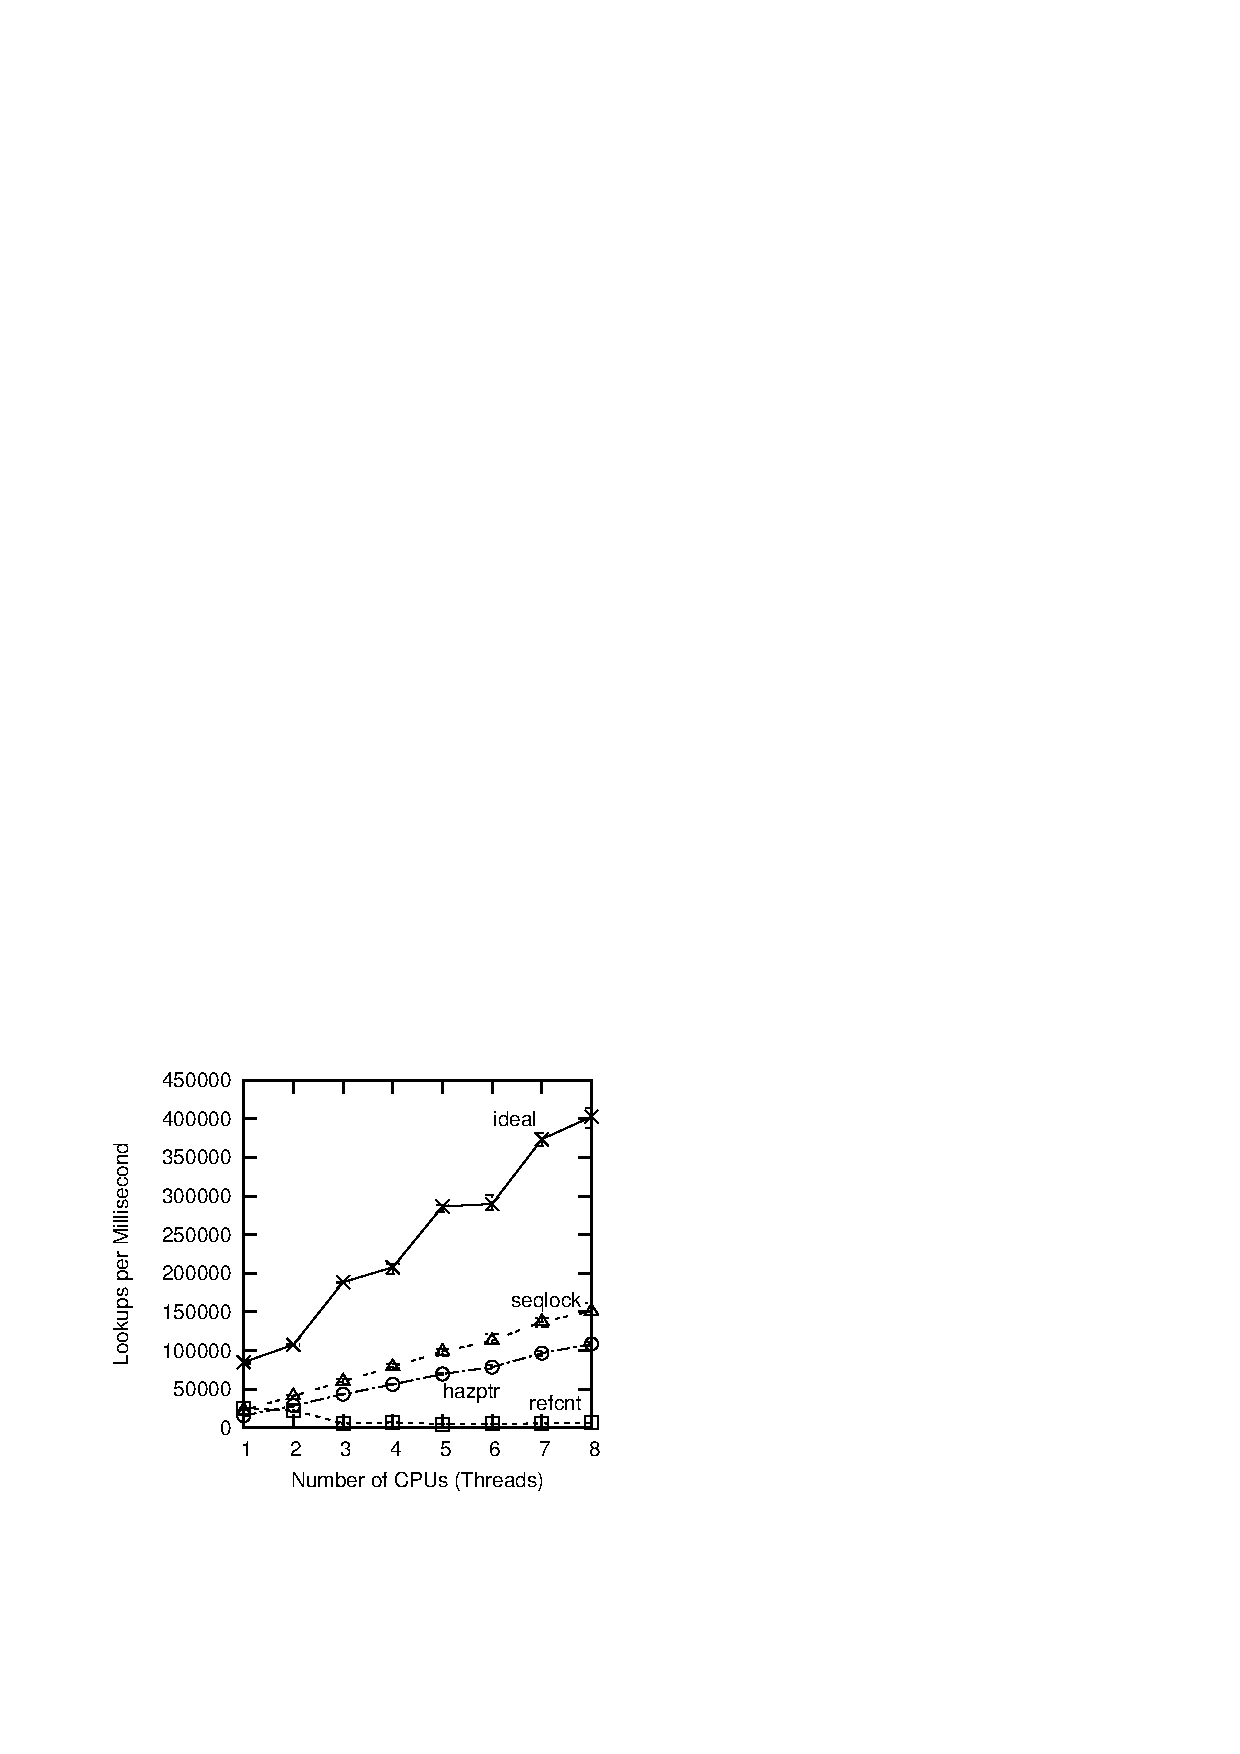
\includegraphics{CodeSamples/defer/perf-seqlock}}
\caption{Pre-BSD Routing Table Protected by Sequence Locking}
\label{fig:defer:Pre-BSD Routing Table Protected by Sequence Locking}
\end{figure}

It also performs better on the read-only workload, as can be seen in
Figure~\ref{fig:defer:Pre-BSD Routing Table Protected by Sequence Locking},
though its performance is still far from ideal.
Worse yet, it suffers use-after-free failures.
The problem is that the reader might encounter a segmentation violation
due to accessing an already-freed structure before \co{read_seqretry()}
has a chance to warn of the concurrent update.

\QuickQuiz{
	Can this bug be fixed?
	In other words, can you use sequence locks as the \emph{only}
	synchronization mechanism protecting a linked list supporting
	concurrent addition, deletion, and lookup?
}\QuickQuizAnswer{
	One trivial way of accomplishing this is to surround all
	accesses, including the read-only accesses, with
	\co{write_seqlock()} and \co{write_sequnlock()}.
	Of course, this solution also prohibits all read-side
	parallelism, resulting in massive lock contention,
	and furthermore could just as easily be implemented
	using simple locking.

	If you do come up with a solution that uses \co{read_seqbegin()}
	and \co{read_seqretry()} to protect read-side accesses, make
	sure that you correctly handle the following sequence of events:

	\begin{enumerate}
	\item	CPU~0 is traversing the linked list, and picks up a pointer
		to list element~A.
	\item	CPU~1 removes element~A from the list and frees it.
	\item	CPU~2 allocates an unrelated data structure, and gets
		the memory formerly occupied by element~A\@.
		In this unrelated data structure, the memory previously
		used for element~A's \co{->next} pointer is now occupied
		by a floating-point number.
	\item	CPU~0 picks up what used to be element~A's \co{->next}
		pointer, gets random bits, and therefore gets a
		segmentation fault.
	\end{enumerate}

	One way to protect against this sort of problem requires use
	of ``type-safe memory'', which will be discussed in
	Section~\ref{sec:defer:RCU Provides Type-Safe Memory}.
	Roughly similar solutions are possible using the hazard pointers
	discussed in
	Section~\ref{sec:defer:Hazard Pointers}.
	But in either case, you would be using some other synchronization
	mechanism in addition to sequence locks!
}\QuickQuizEnd

Both the read-side and write-side critical sections of a sequence lock
can be thought of as transactions, and sequence locking therefore
can be thought of as a limited form of transactional memory, which
will be discussed in Section~\ref{sec:future:Transactional Memory}.
The limitations of sequence locking are: (1)~Sequence locking restricts
updates and (2)~sequence locking does not permit traversal of pointers
to objects that might be freed by updaters.
These limitations are of course overcome by transactional memory, but
can also be overcome by combining other synchronization primitives
with sequence locking.

Sequence locks allow writers to defer readers, but not vice versa.
This can result in unfairness and even starvation
in writer-heavy workloads.\footnote{
	Dmitry Vyukov describes one way to reduce (but, sadly, not eliminate)
	reader starvation:
	\url{http://www.1024cores.net/home/lock-free-algorithms/reader-writer-problem/improved-lock-free-seqlock}.}
On the other hand, in the absence of writers, sequence-lock readers are
reasonably fast and scale linearly.
It is only human to want the best of both worlds: fast readers without
the possibility of read-side failure, let alone starvation.
In addition, it would also be nice to overcome sequence locking's limitations
with pointers.
The following section presents a synchronization mechanism with exactly
these properties.

% rcu.tex
% SPDX-License-Identifier: CC-BY-SA-3.0

\section{Read-Copy Update (RCU)}
\label{sec:defer:Read-Copy Update (RCU)}
%
\epigraph{``Free'' is a \emph{very} good price!}{\emph{Tom Peterson}}

앞의 섹션들에서 다루어진 모든 메커니즘들은 특정 동작을 그것이 안전하게 행해질
수 있을 때까지 유예하는 여러개의 방법들 가운데 하나를 사용했습니다.
Section~\ref{sec:defer:Reference Counting} 에서 다룬 레퍼런스 카운터는 읽기
쓰레드들을 방해할 수 있는 행위들을 유예하기 위해 명시적 카운터를 사용하는데,
이는 읽기 쪽의 혼잡과 그로 말미암은 낮은 확장성을 유발합니다.
Section~\ref{sec:defer:Hazard Pointers} 에서 다루어진 해저드 포인터는
per-thread 포인터 리스트 안의 묵시적 카운터를 사용합니다.
이는 읽기 쪽의 혼잡을 줄입니다만, 읽기 쓰레드들이 쓰기와 조건적 브랜치를
행하고, 읽기 쪽 기능에 전체 메모리 배리어를, 또는 업데이트쪽 기능들의 업데이트
안의 real-time 에 친화적이지 않은 inter-processor 인터럽트를 를 필요로 합니다.
Section~\ref{sec:defer:Sequence Locks} 에서 보인 시퀀스 락 또한 읽기 쪽의
혼잡을 막습니다만, 포인터 traversal 을 보호해주지는 않고, 해저드 포인터처럼
읽기 쪽 기능에 전체 메모리 배리어를 필요로 합니다.
이런 단점은 더 좋은 방법은 없는지에 대한 질문을 이끌어냅니다.
\iffalse

All of the mechanisms discussed in the preceding sections
used one of a number of approaches to defer specific actions
until they may be carried out safely.
The reference counters discussed in
Section~\ref{sec:defer:Reference Counting}
use explicit counters to defer actions that could disturb readers,
which results in read-side contention and thus poor scalability.
The hazard pointers covered by
Section~\ref{sec:defer:Hazard Pointers}
uses implicit counters in the guise of per-thread lists of pointer.
This avoids read-side contention, but requires readers do stores and
conditional branches, as well as either full memory barriers in read-side
primitives or real-time-unfriendly inter-processor interrupts in updates
update-side primitives.
The sequence lock presented in
Section~\ref{sec:defer:Sequence Locks}
also avoids read-side contention, but does not protect pointer
traversals and, like hazard pointers, requires full memory barriers
in read-side primitives.
These schemes' shortcomings raise the question of
whether it is possible to do better.
\fi

이 섹션은 딜레이가 공유된 데이터에의 비싼 업데이트보다는 소스코드에 의해
인식되도록 하는 API 를 제공하는 \emph{read-copy update} (RCU) 를 소개합니다.
이 섹션의 나머지 부분들에서는 여러개의 다른 관점에서 RCU 를 알아봅니다.
Section~\ref{sec:defer:Introduction to RCU} 에서는 RCU 에 대한 고전적인 소개를
제공하고,
Section~\ref{sec:defer:RCU Fundamentals} 에서는 기본적인 RCU 컨셉을 다루며,
Section~\ref{sec:defer:RCU Usage} 에서는 RCU 의 일부 공통적인 사용예를
소개하고,
Section~\ref{sec:defer:RCU Linux-Kernel API} 에서는 리눅스 커널 API 를 보이고,
Section~\ref{sec:defer:RCU Related Work} 에서는 RCU 에 관련된 최근의 것들을
이야기하고, 마지막으로
Section~\ref{sec:defer:RCU Exercises} 에서 일부 RCU 연습을 제공합니다.
\iffalse


This section introduces \emph{read-copy update} (RCU), which provides
an API that allows delays to be identified in the source code,
rather than as expensive updates to shared data.
The remainder of this
section examines RCU from a number of different perspectives.
Section~\ref{sec:defer:Introduction to RCU} provides the classic
introduction to RCU,
Section~\ref{sec:defer:RCU Fundamentals} covers fundamental RCU
concepts,
Section~\ref{sec:defer:RCU Usage} introduces some common uses of RCU,
Section~\ref{sec:defer:RCU Linux-Kernel API} presents the Linux-kernel
API,
Section~\ref{sec:defer:RCU Related Work} covers recent work related
to RCU,
and finally
Section~\ref{sec:defer:RCU Exercises} provides some RCU exercises.
\fi

% defer/rcuintro.tex
% mainfile: ../perfbook.tex
% SPDX-License-Identifier: CC-BY-SA-3.0

\subsection{Introduction to RCU}
\label{sec:defer:Introduction to RCU}

앞의 섹션들에서 이야기된 접근법들은 좋은 확장성을 제공하지만 분명 Pre-BSD
라우팅 테이블에 이상적이진 않은 성능을 제공했습니다.
따라서, ``오직 너무 멀리 가본 사람만이 자기가 얼마나 멀리 갈 수 있는지 안다''
정신에 입각해,\footnote{
	T.~S.~Eliot 에게 사과드립니다.}
동시의 업데이트의 존재에도 불구하고 동시의 읽기 쓰레드들이 싱글 쓰레드
탐색에서와 동일한 어셈블리 언어 인스트럭션들을 수행하는 알고리즘을 통해 더 멀리
가보겠습니다.
물론, 이 칭찬할 만한 목표는 심각한 구현 가능성 질문을 불러일으킬 수
있겠습니다만, 시도도 하지 않으면 성공할 수도 없습니다!

\iffalse

The approaches discussed in the preceding sections have provided
good scalability but decidedly non-ideal performance for the
Pre-BSD routing table.
Therefore, in the spirit of ``only those who have gone too far
know how far you can go'',\footnote{
	With apologies to T.~S.~Eliot.}
we will go all the way, looking into algorithms in which concurrent
readers execute the same sequence of assembly language instructions as
would a single-threaded lookup, despite the presence of concurrent
updates.
Of course, this laudable goal might raise serious implementability
questions, but we cannot possibly succeed if we don't even try!

\fi

\subsubsection{Minimal Insertion and Deletion}
\label{sec:defer:Minimal Insertion and Deletion}

\begin{figure}[tb]
\centering
\resizebox{3in}{!}{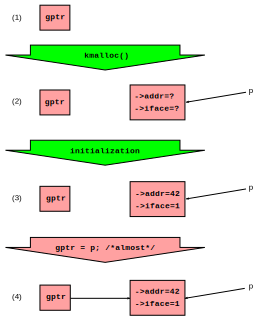
\includegraphics{defer/RCUListInsertClassic}}
\caption{Insertion With Concurrent Readers}
\label{fig:defer:Insertion With Concurrent Readers}
\end{figure}

구현이 가능하긴 한지에 대한 걱정을 최소화 하기 위해, \co{NULL} 이거나 하나의
구조체로의 참조일 하나의 글로벌 포인터로 존재하는 최소한의 데이터 구조에 집중해
봅니다.
이 데이터 구조는 최소한의 것이긴 하지만, 제품 단계에서 상당히 많이 사용되는
것이기도 합니다~\cite{GeoffRomer2018C++DeferredReclamationP0561R4}.
삽입을 위한 고전적 방법이
Figure~\ref{fig:defer:Insertion With Concurrent Readers}
에 보여져 있는데, 위에서 아래로 시간이 흐름에 따라 달라지는 네개의 상태를
보입니다.
첫번째 열은 최초의 상태를 보이는데, \co{gptr} 이 \co{NULL} 입니다.
두번째 열에서, 우리는 물음표로 보여지듯 초기화 되지 않은 이 구조체를
할당합니다.
세번째 열에서, 우린 이 구조체를 초기화 합니다.
마지막으로, 네번째 열에서 우린 \co{gptr} 을 이 새로 할당되고 초기화 된 원소를
참조하도록 업데이트 합니다.

\iffalse

To minimize implementability concerns, we focus on a minimal
data structure, which consists of a single global pointer that is either
\co{NULL} or references a single structure.
Minimal though it might be, this data structure is heavily used in
production~\cite{GeoffRomer2018C++DeferredReclamationP0561R4}.
A classic approach for insertion is shown in
Figure~\ref{fig:defer:Insertion With Concurrent Readers},
which shows four states with time advancing from top to bottom.
The first row shows the initial state, with \co{gptr} equal to \co{NULL}.
In the second row, we have allocated a structure which is uninitialized,
as indicated by the question marks.
In the third row, we have initialized the structure.
Finally, in the fourth and final row, we have updated \co{gptr} to
reference the newly allocated and initialized element.

\fi

우린 이 \co{gptr} 로의 값 할당이 간단한 C-언어의 할당문을 사용할 수 있길 바랄
겁니다.
불행히도,
Section~\ref{sec:toolsoftrade:Shared-Variable Shenanigans}
이 이 바람을 가로막습니다.
따라서, 업데이트 쓰레드는 간단한 C-언어 할당문 대신 이 그림에 보여진 것처럼
\co{smp_store_release()} 또는 뒤에서 보이겠지만 \co{rcu_assign_pointer()} 를
사용해야 합니다.

비슷하게, 어떤 사람들은 읽기 쓰레드가 \co{gptr} 의 값을 얻어오기 위해 하나의
C-언어 할당문을 사용할 수 있기를, 그리고 과거의 값인 \co{NULL} 이나 새로이
설치된 포인터를 읽어와 어떤 경우든 유효한 값을 읽올 것이 보장되기를 바랄
겁니다.
불행히도,
Section~\ref{sec:toolsoftrade:Shared-Variable Shenanigans}
은 이 바람 역시 가로막습니다.
이 보장을 얻기 위해선, 읽기 쓰레드는 그 대신 \co{READ_ONCE()}, 또는, 뒤에서
보이겠지만 \co{rcu_dereference()} 를 사용해야 합니다.
하지만, 대부분의 현대 컴퓨터 시스템에서, 이 읽기 쪽 기능들은 싱글 쓰레드 기반
코드에서 일반적으로 사용될 것과 동일한 하나의 로드 인스트럭션으로 구현될 수
있습니다.

\iffalse

We might hope that this assignment to \co{gptr} could use a simple
C-language assignment statement.
Unfortunately,
Section~\ref{sec:toolsoftrade:Shared-Variable Shenanigans}
dashes these hopes.
Therefore, the updater cannot use a simple C-language assignment, but
must instead use \co{smp_store_release()} as shown in the figure,
or, as will be seen, \co{rcu_assign_pointer()}.

Similarly, one might hope that readers could use a single C-language
assignment to fetch the value of \co{gptr}, and be guaranteed to either
get the old value of \co{NULL} or to get the newly installed pointer,
but either way see a valid result.
Unfortunately, Section~\ref{sec:toolsoftrade:Shared-Variable Shenanigans}
dashes these hopes as well.
To obtain this guarantee, readers must instead use \co{READ_ONCE()},
or, as will be seen, \co{rcu_dereference()}.
However, on most modern computer systems, each of these read-side primitives
can be implemented with a single load instruction, exactly the instruction
that would normally be used in single-threaded code.

\fi

\Cref{fig:defer:Insertion With Concurrent Readers}
를 읽기 쓰레드의 시점에서 다시 보면, 앞의 세개 상태에서 모든 읽기 쓰레드는
\co{gptr} 을 \co{NULL} 값을 갖는 것으로 봅니다.
네번째 상태에 진입하면서, 일부 읽기 쓰레드는 \co{gptr} 이 여전히 \co{NULL} 값을
갖는다고 볼 수 있는 반면 다른 쓰레드들은 새로 설치된 원소를 참조하고 있는
것으로 볼 수 있지만, 어떤 시점 이후로는 모든 읽기 쓰레드가 이 새 원소를 보게 될
겁니다.
항상, 모든 읽기 쓰레드는 \co{gptr} 을 유효한 포인터를 담고 있다고 볼 겁니다.
따라서, 동시의 읽기 쓰레드들이 싱글 쓰레드 기반 코드에서 일반적으로 사용할 것과
동일한 기계 인스트럭션들을 수행하면서 새로운 데이터를 연결된 데이터 구조에
추가하는 것이 정말 가능합니다.
이 동시 읽기에의 비용이 없는 방법은 훌륭한 성능과 확장성을 제공하며, 리얼타임
사용처에서 뛰어나게 잘 사용될 수 있습니다.

\iffalse

Reviewing \cref{fig:defer:Insertion With Concurrent Readers}
from the viewpoint of readers, in the first three states all readers
see \co{gptr} having the value \co{NULL}.
Upon entering the fourth state, some readers might see \co{gptr} still
having the value \co{NULL} while others might see it referencing the
newly inserted element, but after some time, all readers will see this
new element.
At all times, all readers will see \co{gptr} as containing a valid pointer.
Therefore, it really is possible to add new data to linked data structures
while allowing concurrent readers to execute the same sequence of machine
instructions that is normally used in single-threaded code.
This no-cost approach to concurrent reading provides excellent performance
and scalability, and also is eminently suitable for real-time use.

\fi

\begin{figure}[tb]
\centering
\resizebox{3in}{!}{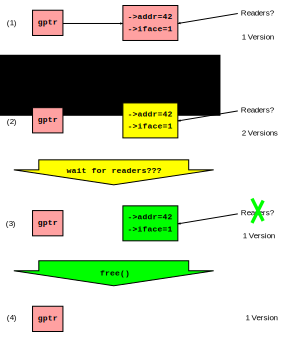
\includegraphics{defer/RCUListDeleteClassic}}
\caption{Deletion With Concurrent Readers}
\label{fig:defer:Deletion With Concurrent Readers}
\end{figure}

삽입은 물론 상당히 유용합니다만, 금방이든 더 나중이든, 데이터를 지워야 하기도
할 겁니다.
Figure~\ref{fig:defer:Deletion With Concurrent Readers}
에 보이듯, 첫번째 단계는 쉽습니다.
Section~\ref{sec:toolsoftrade:Shared-Variable Shenanigans}
에서의 교훈을 다시 상기해 보면, \co{smp_store_release()} 가 이 포인터를
\co{NULL} 로 만들기 위해 사용되어, 이 그림의 첫번째 열에서 두번째 열로
넘어갑니다.
이 시점에서, 기존부터 존재하던 읽기 쓰레드는 \co{->addr} 는 42 값을 그리고
\co{->iface} 는 1 값을 갖는 것으로 볼 수 있지만, 새로 시작된 읽기 쓰레드는
\co{NULL} 포인터를 볼 것으로, 즉 동시의 읽기 쓰레드들이 이 그림의 ``2
Versions'' 로 표시된 것처럼 현 상태에 대해 다른 의견을 가질 수 있습니다.

\iffalse

Insertion is of course quite useful, but sooner or later, it will also
be necessary to delete data.
As can be seen in
Figure~\ref{fig:defer:Deletion With Concurrent Readers},
the first step is easy.
Again taking the lessons from
Section~\ref{sec:toolsoftrade:Shared-Variable Shenanigans}
to heart, \co{smp_store_release()} is used to \co{NULL} the pointer,
thus moving from the first row to the second in the figure.
At this point, pre-existing readers see the old structure with
\co{->addr} of 42 and \co{->iface} of 1, but new readers will see
a \co{NULL} pointer, that is, concurrent readers can disagree on
the state, as indicated by the ``2 Versions'' in the figure.

\fi

\QuickQuizSeries{%
\QuickQuizB{
	Figure~\ref{fig:defer:Deletion With Concurrent Readers}
	는 \co{NULL} 포인터를 저장하는데 왜 \co{smp_store_release()} 를
	사용하나요?
	\co{NULL} 포인터 저장에 대해 순서지을 구조체 초기화가 없다는 점을
	감안하면 \co{WRITE_ONCE()} 만으로도 이 경우에는 괜찮지 않을까요?

	\iffalse

	Why does
	Figure~\ref{fig:defer:Deletion With Concurrent Readers}
	use \co{smp_store_release()} given that it is storing
	a \co{NULL} pointer?
	Wouldn't \co{WRITE_ONCE()} work just as well in this case,
	given that there is no structure initialization to order
	against the store of the \co{NULL} pointer?

	\fi

}\QuickQuizAnswerB{
	맞아요, 그럴 겁니다.

	\co{NULL} 포인터가 할당되고 있을 뿐, 순서지을 것이 존재하지 않으므로,
	\co{smp_store_release()} 를 사용할 필요는없습니다.
	대조적으로, \co{NULL} 이 아닌 포인터를 할당할 때에는 그 포인터로
	가리켜지는 구조체의 초기화가 이 포인터의 할당 전에 행해졌음을 분명히
	하기 위해 \co{smp_store_release()} 가 사용되어야 합니다.

	짧게 말해서, \co{WRITE_ONCE()} 는 동작할 것이고, 어떤 아키텍쳐에서는
	약간의 CPU 시간을 아낄 겁니다.
	하지만, 뒤에서 보게 되겠지만, 소프투에어 엔지니어링 관점의 걱정은
	\co{smp_store_release()} 와 상당히 유사한 \co{rcu_assign_pointer()}
	라는 특수한 기능의 사용을 장려할 겁니다.

	\iffalse

	Yes, it would.

	Because a \co{NULL} pointer is being assigned, there is nothing
	to order against, so there is no need for \co{smp_store_release()}.
	In contrast, when assigning a non-\co{NULL} pointer, it is
	necessary to use \co{smp_store_release()} in order to ensure
	that initialization of the pointed-to structure is carried
	out before assignment of the pointer.

	In short, \co{WRITE_ONCE()} would work, and would
	save a little bit of CPU time on some architectures.
	However, as we will see, software-engineering concerns
	will motivate use of a special \co{rcu_assign_pointer()}
	that is quite similar to \co{smp_store_release()}.

	\fi

}\QuickQuizEndB
%
\QuickQuizE{
	동시에 수행되는 읽기 쓰레드는
	Figure~\ref{fig:defer:Deletion With Concurrent Readers}
	에 그려진 수행 순서에 따르면 \co{gptr} 의 값에 대해 동의하지 않을 수
	있습니다.
	이건 뭔가 문제있지 않나요???

	\iffalse

	Readers running concurrently each other and with the procedure
	outlined in
	Figure~\ref{fig:defer:Deletion With Concurrent Readers}
	can disagree on the value of \co{gptr}.
	Isn't that just a wee bit problematic???

	\fi

}\QuickQuizAnswerE{
	꼭 그렇진 않습니다.

	Section~\ref{sec:cpu:Hardware Optimizations}
	와~\ref{sec:cpu:Hardware Free Lunch?}
	에서 힌트가 주어진 것처럼, 빛의 속도의 지연은 컴퓨터의 데이터는 그
	데이터가 실제로 모델링 하고자 의도된 바깥의 사실에 비교해서는 항상
	오래되어 있습니다.

	따라서 실제 세계의 알고리즘은 외부의 현실과 그 현실을 반영하는 컴퓨터
	내부 데이터의 비일관성을 감내해야만 합니다.
	이런 알고리즘들 여럿은 컴퓨터 내부 데이터에서의 비일관성도 어느정도는
	감내할 수 있습니다.
	Section~\ref{sec:datastruct:RCU-Protected Hash Table Discussion}
	이 이 점을 더 자세히 다룹니다.

	\iffalse

	Not necessarily.

	As hinted at in Sections~\ref{sec:cpu:Hardware Optimizations}
	and~\ref{sec:cpu:Hardware Free Lunch?},
	speed-of-light delays mean that a computer's data is always
	stale compared to whatever external reality that data is intended
	to model.

	Real-world algorithms therefore absolutely must tolerate
	inconsistancies between external reality and the in-computer
	data reflecting that reality.
	Many of those algorithms are also able to tolerate some degree
	of inconsistency within the in-computer data.
	Section~\ref{sec:datastruct:RCU-Protected Hash Table Discussion}
	discusses this point in more detail.

	\fi

	이런 비일관적이고 오래된 데이터를 감내해야 하는 필요성은 RCU 에만
	국한되지 않는다는 점을 알아두시기 바랍니다.
	이는 레퍼런스 카운팅, 해저드 포인터, 시퀀스 락, 그리고 심지어 일부 락킹
	사용 예에도 적용됩니다.
	예를 들어, 여러분이 락을 잡은 채 어떤 값을 계산하지만 그 값을 해당 락을
	해제한 후 사용한다면, 여러분은 오래된 데이터를 사용하고 있을 수
	있습니다.
	어쨌건, 그 값이 기반하고 있는 데이터는 그 락이 해제되는 순간 어떻게든
	변할 수도 있습니다.

	그러니, 그렇습니다, RCU 읽기 쓰레드는 오래되고 비일관적인 데이터를 볼
	수 있습니다, 하지만 아니요, 이게 문제여야만 할 이유는 없어요.
	그리고 필요하다면 그런 오래되고 비일관적인 데이터 문제를 막을 수 있는
	RCU 사용 패턴도 있습니다~\cite{Arcangeli03}.

	\iffalse

	Please note that this need to tolerate inconsistent and stale
	data is not limited to RCU\@.
	It also applies to reference counting, hazard pointers, sequence
	locks, and even to some locking use cases.
	For example, if you compute some quantity while holding a lock,
	but use that quantity after releasing that lock,
	you might well be using stale data.
	After all, the data that quantity is based on might change
	arbitrarily as soon as the lock is released.

	So yes, RCU readers can see stale and inconsistent data, but no,
	this is not necessarily problematic.
	And, when needed, there are RCU usage patterns that avoid both
	staleness and inconsistency~\cite{Arcangeli03}.

	\fi

}\QuickQuizEndE
}

우린 열~3 에서 볼 수 있듯 모든 기존부터 존재한 읽기 쓰레드들이 완료하길
기다리는 것만으로 단일 버전으로 돌아올 수 있습니다.
이 지점에서, 모든 기존부터 존재하던 읽기 쓰레드는 종료되었고, 뒤따르는 읽기
쓰레드는 어느 것도 기존 데이터 아이템으로의 경로를 갖지 못하므로, 그걸 참조하는
어떤 읽기 쓰레드도 존재할 수 없습니다.
따라서 그 아이템은 열~4 에서 보여지듯 안전히 메모리 해제될 수 있습니다.

따라서, 기존부터 존재한 읽기 쓰레드들이 완료되길 기다릴 방법이 존재한다면
읽기 쓰레드들이 싱글 쓰레드 수행 시에나 적합할 것과 동일한 기계
인스트럭션들만을 수행하면서도 연결된 데이터 구조에 데이터를 추가할 수도 삭제할
수도 있습니다.
그러니 앞서 했던 것들이 너무 멀리 간 것만은 아닐수도 있습니다!

하지만 어떻게 기존부터 존재한 읽기 쓰레드들이 실제로 완료되었다고 이야기 할 수
있을까요?
이 질문이 다음 섹션의 주제입니다.

\iffalse

We get back to a single version simply by waiting for all the
pre-existing readers to complete, as shown in row~3.
At that point, all the pre-existing readers are done, and no later
reader has a path to the old data item, so there can no longer be
any readers referencing it.
It may therefore be safely freed, as shown on row~4.

Thus, given a way to wait for pre-existing readers to complete,
it is possible to both add data to and remove data from a linked
data structure, despite the readers executing the same sequence
of machine instructions that would be appropriate for single-threaded
execution.
So perhaps going all the way was not too far after all!

But how can we tell when all of the pre-existing readers have in
fact completed?
This question is the topic of the next section.

\fi

\subsubsection{Waiting for Readers}
\label{sec:defer:Waiting for Readers}

읽기 쓰레드의 기다리기를 레퍼런스 카운팅 기반으로 하고 싶을 수 있겠습니다만,
Chapter~\ref{chp:Counting}
의
Figure~\ref{fig:count:Atomic Increment Scalability on x86}
는 현재의 레퍼런스 카운팅은
Section~\ref{sec:defer:Reference Counting}
에서 이미 보았듯 굉장한 오버헤드를 초래함을 보았습니다.
해저드 포인터는 이 오버헤드를 상당히 줄입니다만, 우리가
Section~\ref{sec:defer:Hazard Pointers}
에서 보았듯이, 완전히 없애진 못합니다.
그렇다고는 하나, 많은 RCU 구현이 매우 주의 깊은 캐시 지역적 카운터의 사용을
합니다.

\iffalse

It is tempting to base reader waiting on reference counting, but
Figure~\ref{fig:count:Atomic Increment Scalability on x86}
in
Chapter~\ref{chp:Counting}
shows that concurrent reference counting results in extreme overhead,
as we already saw in
Section~\ref{sec:defer:Reference Counting}.
Hazard pointers profoundly reduce this overhead, but, as we saw in
Section~\ref{sec:defer:Hazard Pointers}, not to zero.
Nevertheless, many RCU implementations make very careful cache-local
use of counters.

\fi

두번째 접근법은 메모리 동기화가 비쌈을 파악하고, 따라서 레지스터를 대신
사용하는데, 이는 각 CPU 또는 쓰레드의 프로그램 카운터 (PC) 로, 따라서 읽기
쓰레드에게는 적어도 동시의 업데이트의 부재 시에는 오버헤드를 일으키지 않습니다.
업데이트 쓰레드는 각 적절한 PC 를 반복적으로 살펴보고, 그 PC 가 읽기 쪽 코드
내에 위치해 있지 않다면, 연관된 CPU 또는 쓰레드는 조용한 상태 (quiescent state)
에 있는 것이며, 따라서 이는 새로이 제거된 데이터 원소로의 액세스를 할수도 있는
읽기 쓰레드는 모두 완료되었다는 신호가 됩니다.
모든 CPU 또는 쓰레드의 PC 가 모두 모든 읽기 쓰레드의 바깥에 있음이 확인된다면,
이 유예 기간 (grace period) 가 완료됩니다.
이 방법은 몇가지 심각한 기술적 어려움도 가지고 있는데, 메모리 순서 맞추기, 읽기
쓰레드에 의해 \emph{가끔} 호출되는 함수들, 그리고 항상 신나는 코드 모습
최적화가 포함됩니다.
그러나, 이 방법은 제품 단계에서 사용되었다고 이야기
됩니다~\cite{MikeAsh2015Apple}.

\iffalse

A second approach observes that memory synchronization is expensive,
and therefore uses registers instead, namely each CPU's or thread's
program counter (PC), thus imposing no overhead on readers, at least
in the absence of concurrent updates.
The updater polls each relevant PC, and if that PC is not within read-side
code, then the corresponding CPU or thread is within a quiescent state,
in turn signaling the completion of any reader that might have access
to the newly removed data element.
Once all CPU's or thread's PCs have been observed to be outside of any
reader, the grace period has completed.
Please note that this approach poses some serious challenges, including
memory ordering, functions that are \emph{sometimes} invoked from readers,
and ever-exciting code-motion optimizations.
Nevertheless, this approach is said to be used in
production~\cite{MikeAsh2015Apple}.

\fi

세번째 접근법은 모든 합리적 읽기 쓰레드의 수명을 충분히 넘어설 정도로 긴 고정된
시간동안 그냥 기다리는 것입니다~\cite{Jacobson93,AjuJohn95}.
이는 하드 리얼타임 시스템에서는 잘 동작합니다만~\cite{YuxinRen2018RTRCU},
그보다 덜 진귀한 환경에서라면, Murphy 는 비합리적일 정도로 오래 살아있는 읽기
쓰레드에도 준비해야 하는게 무척 중요하다고 말합니다.
이를 자세히 보기 위해, 그러는데 실패했을 때의 결과를 생각해 봅시다:
어떤 데이터 항목은 이 비합리적인 읽기 쓰레드가 여전히 그것을 참조하고 있는 동안
메모리 해제될 수 있고, 그 항목은 곧바로 재할당되어 심지어 다른 타입의 데이터
항목으로 사용되고 있을 수 있습니다.
그러면 이 비합리적 읽기 쓰레드와 부주의한 재할당자는 같은 메모리를 두개의 매우
다른 목적으로 사용하려 할 것입니다.
그 결과는 디버깅 하기에 무척 어려울 것입니다.

\iffalse

A third approach is to simply wait for a fixed period of time that is
long enough to comfortably exceed the lifetime of any reasonable
reader~\cite{Jacobson93,AjuJohn95}.
This can work quite well in hard real-time systems~\cite{YuxinRen2018RTRCU},
but in less exotic
settings, Murphy says that it is critically important to be prepared
even for unreasonably long-lived readers.
To see this, consider the consequences of failing do so:
A data item will be freed while the unreasonable reader is still
referencing it, and that item might well be immediately reallocated,
possibly even as a data item of some other type.
The unreasonable reader and the unwitting reallocator would then
be attempting to use the same memory for two very different purposes.
The ensuing mess will at best be exceedingly difficult to debug.

\fi

네번째 접근법은 영원히 기다리는 것으로, 그렇게 하는게 가장 비합리적인 읽기
쓰레드조차도 처리해 줄 것이라는 점에서 안전합니다.
이 접근법은 또한 ``메모리 누출'' 이라고도 불리며, 메모리 누출은 시기 상조의
그리고 불편한 리부팅을 요구한다는 사실 때문에 나쁜 평판을 가지고 있습니다.
그러나, 이는 업데이트 비율과 시스템 가동시간이 모두 꽤 정확히 그 한계가 정해져
있을 때라면 사용될 수 있는 전략입니다.
예를 들어, 이 방법은 시스템이 높은 가용성을 가진 클러스터여서 이 클러스터가
정말로 높은 가용성을 유지한다는 것을 분명히 하기 위해 주기적으로 고장나는
것이라면 잘 동작할 수 있습니다.\footnote{
	이 주기적 고장을 강제하는 프로그램은 가끔 ``chaos monkey'' 라고
	불립니다:
	\url{https://netflix.github.io/chaosmonkey/}.
	하지만, 너무 오래 수행되는 시스템에 의해 야기되는 혼란을 무시하는 것도
	실수가 될수도 있습니다.}
메모리를 누출하는 것은 또한 garbage collector 를 가진 경우에도 사용될 수
있을텐데, 이 경우는 garbage collector 가 이 누출을 막는 것으로 생각될 수
있습니다~\cite{Kung80}.
하지만, 여러분의 환경이 garbage collector 를 지원하지 않는다면, 마저
읽으십시오!

\iffalse

A fourth approach is to wait forever, secure in the knowledge that
doing so will accommodate even the most unreasonable reader.
This approach is also called ``leaking memory'', and has a bad reputation
due to the fact that memory leaks often require untimely and
inconvenient reboots.
Nevertheless, this is a viable strategy when the update rate and the
uptime are both sharply bounded.
For example, this approach could work well in a high-availability
cluster where systems were periodically crashed in order to ensure
that cluster really remained highly available.\footnote{
	The program that forces the periodic crashing is sometimes
	known as a ``chaos monkey'':
	\url{https://netflix.github.io/chaosmonkey/}.
	However, it might also be a mistake to neglect chaos caused
	by systems running for too long.}
Leaking the memory is also a viable strategy in environments having
garbage collectors, in which case the garbage collector can be thought
of as plugging the leak~\cite{Kung80}.
However, if your environment lacks a garbage collector, read on!

\fi

다섯번째 접근법은 전통적 세상을-멈추기 (stop-the-world) garbage collector 에
의해 예시되는 주기적으로 ``세상을 멈추기'' 를 사용해 주기적 고장내기를
막습니다.
이 방법은 또한 각 일하는 날의 끝마다 시스템의 전원을 끄는게 일반적 행동이었던,
어디나 있는 연결성 전의 수십년간 많이 사용되었습니다.
하지만, 오늘날의 항상 연결되어 있고 항상 켜져있는 세상에서는, 세상을 멈추기는
응답 시간을 크게 악화시킬 수 있는데, 이는 동시적 garbage collector 의 개발의
모티베이션 중 하나가 되었습니다~\cite{DavidFBacon2003RTGC}.
더 나아가, 우린 모든 앞서서부터 존재하고 있는 읽기 쓰레드가 모두 완료되기를
기다려야 하기는 하지만, 그것들이 동시에 완료되어야 할 필요는 없습니다.

\iffalse

A fifth approach avoids the period crashes in favor of periodically
``stopping the world'', as exemplified by the traditional stop-the-world
garbage collector.
This approach was also heavily used during the decades before
ubiquitous connectivity, when it was common practice to power systems
off at the end of each working day.
However, in today's always-connected always-on world, stopping the world
can gravely degrade response times, which has been one motivation for the
development of concurrent garbage collectors~\cite{DavidFBacon2003RTGC}.
Furthermore, although we need all pre-existing readers to complete, we do
not need them all to complete at the same time.

\fi

이 발견은 여섯번째 접근법을 이끌어내는데, 한번에 한 CPU 또는 쓰레드를 멈추는
것입니다.
이 방법은 읽기 쓰레드의 응답 시간을 전혀 악화시키지 않는다는 장점을 갖습니다.
더 나아가서, 많은 어플리케이션들이 이미 앞의 앞서서부터 존재하고 있는 읽기
스레드들이 모두 완료된 후에만 도달할 수 있는 상태 (\emph{quiescent state} 라
불립니다) 를 갖습니다.
트랜잭션 처리 시스템에서는, 한쌍의 연속된 트랜잭션 사이의 시간이 quiescent
state 일 수 있습니다.
반응형 시스템에서는, 연속된 한 쌍의 이벤트 사이의 상태가 quiescent state 일
겁니다.
Preemption 기반이지 않은 운영체제 커널에서는, 컨텍스트 스위치가 quiescent state
가 될 수 있습니다~\cite{McKenney98}.
어떤 형태든, 모든 CPU 그리고/또는 쓰레드가 하나의 quiescent state 를 지난다면,
이 시스템은 하나의 \emph{grace period} 를 완료했다고 이야기 되며, 이 지점에서는
이 grace period 의 시작 시점에서 존재했던 모든 읽기 쓰레드는 완료되었다는게
보장됩니다.
그 결과, 이 grace period 의 시작 전에 제거된 데이터 항목들은 메모리 해제되기에
안전합니다.\footnote{
	RCU 는 단순히 메모리 회수 미루기보다 훨씬 많은 걸 할 수 있으나, 
	회수 미루기는 RCU 의 가장 흔한 사용예이며, 따라서 시작하기에 훌륭한
	지점입니다.}

\iffalse

This observation leads to the sixth approach, which is stopping
one CPU or thread at a time.
This approach has the advantage of not degrading reader response times
at all, let alone gravely.
Furthermore, numerous applications already have states (termed
\emph{quiescent states}) that can be
reached only after all pre-existing readers are done.
In transaction-processing systems, the time between a pair of
successive transactions might be a quiescent state.
In reactive systems, the state between a pair of successive events
might be a quiescent state.
Within non-preemptive operating-systems kernels, a context switch can be
a quiescent state~\cite{McKenney98}.
Either way, once all CPUs and/or threads have passed through a quiescent
state, the system is said to have completed a \emph{grace period},
at which point all readers in existence at the start of that grace period
are guaranteed to have completed.
As a result, it is also guaranteed to be safe to free any removed data
items that were removed prior to the start of that grace period.\footnote{
	It is possible to do much more with RCU than simply defer
	reclamation of memory, but deferred reclamation is RCU's most
	common use case, and is therefore an excellent place to start.}

\fi

Preemption 이 없는 운영체제 커널에서 컨텍스트 스위치가 유효한 quiescent state 가 되려면 읽기 쓰레드는
Figure~\ref{fig:defer:Insertion With Concurrent Readers}
와~\ref{fig:defer:Deletion With Concurrent Readers}
의 \co{gptr} 포인터에 의해 얻어지는 데이터 구조 인스턴스를 참조하는 동안은
블록킹 되는 걸 방지해야만 합니다.
이 블록킹 방지 제약은 순수 스핀락에서도 비슷한 제약으로 존재하는데, 여기선 CPU
는 스핀락을 잡고 있는 동안 블록킹 되는게 금지됩니다.
이 제약이 없다면, 모든 CPU 는 블록된 쓰레드에 의해 잡혀 있는 스핀락을 획득하려
스핀하는 쓰레드들에 의해 소모될 수 있습니다.
이 스핀하는 쓰레드들은 그것들이 이 락을 획득하기 전까지는 CPU 를 놓지 않을
것이지만, 이 락을 쥐고 있는 쓰레드는 이 스핀하고 있는 쓰레드들 중 하나가 CPU 를
하나라도 놓기 전까지는 이 락을 놓아주지 못할 겁니다.
이는 고전적 데드락 환경이며, 이 데드락은 스핀락을 잡고 있는 동안은 블록킹을
방지하는 것으로 막아집니다.

\iffalse

Within a non-preemptive operating-system kernel, for context switch to be
a valid quiescent state, readers must be prohibited from blocking while
referencing a given instance data structure obtained via the \co{gptr}
pointer shown in
Figures~\ref{fig:defer:Insertion With Concurrent Readers}
and~\ref{fig:defer:Deletion With Concurrent Readers}.
This no-blocking constraint is consistent with similar constraints
on pure spinlocks, where a CPU is forbidden from blocking while
holding a spinlock.
Without this constraint, all CPUs might be consumed by threads
spinning attempting to acquire a spinlock held by a blocked thread.
The spinning threads will not relinquish their CPUs until they acquire
the lock, but the thread holding the lock cannot possibly release it
until one of the spinning threads relinquishes a CPU\@.
This is a classic deadlock situation, and this deadlock is avoided
by forbidding blocking while holding a spinlock.

\fi

다시, 이 동일한 제약이 \co{gptr} 을 역참조하는 읽기 쓰레드에게도 적용됩니다:
그런 쓰레드는 그것들이 이 가리켜진 데이터 항목을 사용하는 것을 마무리 하기
전까지는 블록되지 않아야 합니다.
업데이트 쓰레드가 막 \co{smp_store_release()} 를 수행하는 것을 완료한
Figure~\ref{fig:defer:Deletion With Concurrent Readers}
의 두번째 열로 돌아와서, CPU~0 이 컨텍스트 스위치를 했다고 생각해 봅시다.
읽기 쓰레드는 이 링크드 리스트를 순회하는 동안은 블록되는 것이 허용되지
않았으므로, 우린 CPU~0 에서 수행되었을 수도 있는 모든 앞의 읽기 쓰레드들이
완료되었다고 보장됩니다.
이 논리를 다른 CPU 들로 확장하면, 각 CPU 가 모두 컨텍스트 스위치 수행을
목격했다면, 모든 앞의 읽기 쓰레드가 완료되었음이, 새로이 제거된 데이터 원소를
참조하고 있는 어떤 읽기 쓰레드도 더이상 존재하지 않음이 보장됩니다.
그럼 이 업데이트 쓰레드는 안전하게 이 데이터 원소를 메모리 해제할 수 있어,
Figure~\ref{fig:defer:Deletion With Concurrent Readers}
의 가장 아래에 보인 상태에 도달합니다.

\iffalse

Again, this same constraint is imposed on reader threads dereferencing
\co{gptr}: such threads are not allowed to block until after
they are done using the pointed-to data item.
Returning to the second row of
Figure~\ref{fig:defer:Deletion With Concurrent Readers},
where the updater has just completed executing the \co{smp_store_release()},
imagine that CPU~0 executes a context switch.
Because readers are not permitted to block while traversing the linked
list, we are guaranteed that all prior readers that might have been running on
CPU~0 will have completed.
Extending this line of reasoning to the other CPUs, once each CPU has
been observed executing a context switch, we are guaranteed that all
prior readers have completed, and that there are no longer any reader
threads referencing the newly removed data element.
The updater can then safely free that data element, resulting in the
state shown at the bottom of
Figure~\ref{fig:defer:Deletion With Concurrent Readers}.

\fi

\begin{figure}[tb]
\centering
\resizebox{3in}{!}{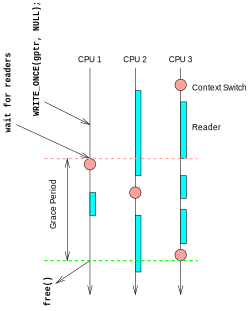
\includegraphics{defer/QSBRGracePeriod}}
\caption{QSBR: Waiting for Pre-Existing Readers}
\label{fig:defer:QSBR: Waiting for Pre-Existing Readers}
\end{figure}

이 방법은 \emph{quiescent state based reclamation}
(QSBR)~\cite{ThomasEHart2006a} 라고 명명되었습니다.
하나의 QSBR 방법이
Figure~\ref{fig:defer:QSBR: Waiting for Pre-Existing Readers}
에 시간이 이 그림의 꼭대기에서 아래로 흐르는 모습으로 그려져 있습니다.
CPU~1 은 현재 데이터 항목을 제거하는 \co{WRITE_ONCE()} 를 수행하고 (아마도 이
포인터 값을 앞서 읽었고 자신을 적절한 동기화를 하고 있게 했을 겁니다), 읽기
쓰레드를 기다립니다.
이 대기 오퍼레이션은 즉각적인 컨텍스트 스위치를 초래하는데, 이는 quiescent
state 로 (핑크색 원으로 표시되어 있습니다), CPU~1 에서의 모든 앞선 읽기는
완료되었음을 의미합니다.
이어서, CPU~2 가 컨텍스트 스위치를 하여, CPU~1 과~2 의 모든 읽기 쓰레드는 이제
완료되었음이 알려집니다.
마지막으로, CPU~3 이 컨텍스트 스위치를 합니다.
이 지점에서, 전체 시스템의 모든 읽기 쓰레드는 완료되었음이 알려지며, 따라서
grace period 가 종료되어 CPU~1 이 오래된 데이터 항목을 메모리 해제하는 것을
허용합니다.

\iffalse

This approach is termed \emph{quiescent state based reclamation}
(QSBR)~\cite{ThomasEHart2006a}.
A QSBR schematic is shown in
Figure~\ref{fig:defer:QSBR: Waiting for Pre-Existing Readers},
with time advancing from the top of the figure to the bottom.
CPU~1 does the \co{WRITE_ONCE()} that removes the current data
item (presumably having previously read the pointer value and
availed itself of appropriate synchronization), then waits
for readers.
This wait operation results in an immediate context switch, which is a
quiescent state (denoted by the pink circle), which in turn means that
all prior reads on CPU~1 have completed.
Next, CPU~2 does a context switch, so that all readers on CPUs~1 and~2
are now known to have completed.
Finally, CPU~3 does a context switch.
At this point, all readers throughout the entire system are known to
have completed, so the grace period ends, permitting CPU~1 to free
the old data item.

\fi

\QuickQuiz{
	Figure~\ref{fig:defer:QSBR: Waiting for Pre-Existing Readers} 에서,
	CPU~3 의 이 오래된 데이터 항목으로의 액세스를 했을 수 있는 읽기
	쓰레드는 이 grace period 가 시작하기도 전에 이미 완료되었어요!
	그런데 왜 CPU~3 의 마지막 컨텍스트 스위치를 신경쓰나요???

	\iffalse

	In Figure~\ref{fig:defer:QSBR: Waiting for Pre-Existing Readers},
	the last of CPU~3's readers that could possibly have
	access to the old data item ended before the grace period
	even started!
	So why would anyone bother waiting until CPU~3's later context
	switch???

	\fi

}\QuickQuizAnswer{
	이 대기는 읽기 쓰레드들이 싱글쓰레드 상황에서나 적절한 것과 똑같은
	인스트럭션들을 사용할 수 있게 해주기 때문입니다.
	달리 말하자면, 이 추가적인 ``과잉의'' 대기가 읽기 쪽의 훌륭한 성능,
	확장성, 그리고 리얼타임 응답을 가능하게 합니다.

	\iffalse

	Because that waiting is exactly what enables readers to use
	the same sequence of instructions that is appropriate for
	single-theaded situations.
	In other words, this additional ``redundant'' waiting enables
	excellent read-side performance, scalability, and real-time
	response.

	\fi

}\QuickQuizEnd

\subsubsection{Toy Implementation}
\label{sec:defer:Toy Implementation}

제품 수준 QSBR 구현은 무척 복잡할 수 있지만, preemption 기반이 아닌 리눅스
커널에서의 장난감 수준 구현은 굉장히 간단합니다:

\iffalse

Although production-quality QSBR implementations can be quite complex,
a toy non-preemptive Linux-kernel implementation is exceedingly simple:

\fi

\begin{VerbatimN}[samepage=true]
void synchronize_rcu(void)
{
	int cpu;

	for_each_online_cpu(cpu)
		sched_setaffinity(current->pid, cpumask_of(cpu));
}
\end{VerbatimN}

\co{for_each_online_cpu()} 기능은 모든 CPU 를 순회하고,
\co{sched_setaffinity()} 함수는 현재 쓰레드가 명시된 CPU 에서 수행되게 하는데,
이는 이 대상 CPU 가 컨텍스트 스위치를 수행하게끔 강제합니다.
따라서, \co{for_each_online_cpu()} 가 완료되고 나면, 각 CPU 는 한번의 컨텍스트
스위치는 수행한 것인데, 이는 곧 모든 앞서서부터 존재해온 읽기 쓰레드가 모두
완료되었음을 보장합니다.

\iffalse

The \co{for_each_online_cpu()} primitive iterates over all CPUs, and
the \co{sched_setaffinity()} function causes the current thread to
execute on the specified CPU, which forces the destination CPU to execute
a context switch.
Therefore, once the \co{for_each_online_cpu()} has completed, each CPU
has executed a context switch, which in turn guarantees that
all pre-existing reader threads have completed.

\fi

\begin{listing}[tbp]
\begin{fcvlabel}[ln:defer:Insertion and Deletion With Concurrent Readers]
\begin{VerbatimL}[commandchars=\\\[\]]
struct route *gptr;

int access_route(int (*f)(struct route *rp))
{
	int ret = -1;
	struct route *rp;

	rcu_read_lock();
	rp = rcu_dereference(gptr);
	if (rp)
		ret = f(rp);		\lnlbl[access_rp]
	rcu_read_unlock();
	return ret;
}

struct route *ins_route(struct route *rp)
{
	struct route *old_rp;

	spin_lock(&route_lock);
	old_rp = gptr;
	rcu_assign_pointer(gptr, rp);
	spin_unlock(&route_lock);
	return old_rp;
}

int del_route(void)
{
	struct route *old_rp;

	spin_lock(&route_lock);
	old_rp = gptr;
	RCU_INIT_POINTER(gptr, NULL);
	spin_unlock(&route_lock);
	synchronize_rcu();
	free(old_rp);
	return !!old_rp;
}
\end{VerbatimL}
\end{fcvlabel}
\caption{Insertion and Deletion With Concurrent Readers}
\label{lst:defer:Insertion and Deletion With Concurrent Readers}
\end{listing}

이 방법은 제품 수준이 \emph{아님을} 알아 두시기 바랍니다.
여러개의 특수 상황에 대한 처리와 여러개의 강력한 최적화의 필요는 제품 수준
구현이 무척 복잡함을 의미합니다.
이에 더해, preemption 기반 환경을 위한 RCU 구현은 읽기 쓰레드가 실제로 무언가를
더할 것을 필요로 하는데, 리얼타임이 아닌 리눅스 커널 환경에서는
\co{rcu_read_lock()} 과 \co{rcu_read_unlock()} 을 각각 \co{preempt_disable()}
과 \co{preempt_enable()} 로 간단히 정의하는 것으로 될 수 있습니다.\footnote{
	Preemption 되는 읽기쪽 크리티컬 섹션을 다루는 어떤 장난감 수준 RCU
	구현들이 Appendix~\ref{chp:app:``Toy'' RCU Implementations} 에 보여져
	있습니다.}
그러나, 이 간단한 preemption 불가 방법은 이론적으로 완벽하며, 읽기 쪽 동기화를
동시의 업데이트가 있음에도 불구하고 비용 없이 제공하는게 가능함을 보입니다.
실제로,
Listing~\ref{lst:defer:Insertion and Deletion With Concurrent Readers}
은 어떻게 읽기 (\co{access_route()}),
Figure~\ref{fig:defer:Insertion With Concurrent Readers} 의 삽입,
(\co{ins_route()})
Figure~\ref{fig:defer:Deletion With Concurrent Readers} 의 삭제가
(\co{del_route()} 구현될 수 있는지 보입니다.
(약간 더 그럴싸한 라우팅 테이블은
Section~\ref{sec:defer:RCU for Pre-BSD Routing} 에 보여져 있습니다.)

\iffalse

Please note that this approach is \emph{not} production quality.
Correct handling of a number of corner cases and the need for a number
of powerful optimizations mean that production-quality implementations
are quite complex.
In addition, RCU implementations for preemptible environments
require that readers actually do something, which in non-real-time
Linux-kernel environments can be as simple as defining
\co{rcu_read_lock()} and \co{rcu_read_unlock()} as \co{preempt_disable()}
and \co{preempt_enable()}, respectively.\footnote{
	Some toy RCU implementations that handle preempted
	read-side critical sections are shown in
	Appendix~\ref{chp:app:``Toy'' RCU Implementations}.}
However, this simple non-preemptible approach is conceptually complete,
and demonstrates that it really is possible to provide read-side
synchronization at zero cost, even in the face of concurrent updates.
In fact,
Listing~\ref{lst:defer:Insertion and Deletion With Concurrent Readers}
shows how reading (\co{access_route()}),
Figure~\ref{fig:defer:Insertion With Concurrent Readers}'s
insertion (\co{ins_route()}) and
Figure~\ref{fig:defer:Deletion With Concurrent Readers}'s
deletion (\co{del_route()}) can
be implemented.
(A slightly more capable routing table is shown in
Section~\ref{sec:defer:RCU for Pre-BSD Routing}.)

\fi

\QuickQuizSeries{%
\QuickQuizB{
	Listing~\ref{lst:defer:Insertion and Deletion With Concurrent Readers}
	의 \co{rcu_read_lock()} 과 \co{rcu_read_unlock()} 의 요점이 뭔가요?
	이 quiescent state 들이 스스로 자신을 이야기하게 하는건 어떤가요?

	\iffalse

	What is the point of \co{rcu_read_lock()} and \co{rcu_read_unlock()} in
	Listing~\ref{lst:defer:Insertion and Deletion With Concurrent Readers}?
	Why not just let the quiescent states speak for themselves?

	\fi

}\QuickQuizAnswerB{
	읽기 쓰레드들은 quiescent state 를 가로지를 수 없음을 기억하세요.
	예를 들어, 리눅스 커널에서 RCU 읽기 쓰레드는 컨텍스트 스위치를 수행할
	수 없습니다.
	\co{rcu_read_lock()} 과 \co{rcu_read_unlock()} 의 사용은 올바르지 않게
	위치된 quiescent state 들을 디버깅 할 수 있게 하고, 그러지 않으면 찾기
	어렵고 간헐적으로 나타나며 무척 파괴적인 버그를 찾기 쉽게 해줍니다.

	\iffalse

	Recall that readers are not permitted to pass through a quiescent
	state.
	For example, within the Linux kernel, RCU readers are not permitted
	to execute a context switch.
	Use of \co{rcu_read_lock()} and \co{rcu_read_unlock()} enables
	debug checks for improperly placed quiescent states, making it
	easy to find bugs that would otherwise be difficult to find,
	intermittent, and quite destructive.

	\fi

}\QuickQuizEndB
%
\QuickQuizE{
	Listing~\ref{lst:defer:Insertion and Deletion With Concurrent Readers}
	의 \co{rcu_dereference()}, \co{rcu_assign_pointer()}, 그리고
	\co{RCU_INIT_POINTER()} 의 요점이 뭔가요?
	그냥 \co{READ_ONCE()}, \co{smp_store_release()}, 그리고
	\co{WRITE_ONCE()} 를 각각 대신 사용하는 건 어떤가요?

	\iffalse

	What is the point of \co{rcu_dereference()}, \co{rcu_assign_pointer()}
	and \co{RCU_INIT_POINTER()} in
	Listing~\ref{lst:defer:Insertion and Deletion With Concurrent Readers}?
	Why not just use \co{READ_ONCE()}, \co{smp_store_release()}, and
	\co{WRITE_ONCE()}, respectively?

	\fi

}\QuickQuizAnswerE{
	RCU 특정 API 들은 제안된 교체와 실제로 비슷한 의미를 가집니다만, RCU
	특정 API 가 RCU 포인터가 아닌 것들에 대해 호출되었을 때, 그리고 그
	거꾸로인 상황에 문제를 제기하는 정적 분석 디버깅 검사를 가능하게
	합니다.

	\iffalse

	The RCU-specific APIs do have similar semantics to the suggested
	replacements, but also enable static-analysis debugging checks
	that complain if an RCU-specific API is invoked on a non-RCU
	pointer and vice versa.

	\fi

}\QuickQuizEndE
}

Listing~\ref{lst:defer:Insertion and Deletion With Concurrent Readers}
으로 돌아가서, \co{route_lock} 이 \co{ins_route()} 와 \co{del_route()} 를
호출하는 동시의 업데이트들 사이의 동기화를 위해 사용되었음을 알아두시기
바랍니다.
하지만, 이 락은 \co{access_route()} 를 호출하는 읽기 쓰레드에 의해서는 획득되지
않습니다:
읽기 쓰레드들은 그대신
\cref{sec:defer:Waiting for Readers} 에서 이야기 된 QSBR 기법을 통해
보호됩니다.

\co{ins_route()} 는
Figure~\ref{fig:defer:Insertion With Concurrent Readers} 가 항상 \co{NULL} 일
거라고 가정하는 \co{gptr} 의 기존 값을 리턴할 뿐임을 알아 두시기 바랍니다.
이는 \co{NULL} 이 아닌 값을 가지고 뭘 할지 알아내는 건 호출자의 책임이며, 읽기
쓰레드들이 확정되지 않은 기간동안 그에 대한 참조를 하고 있을 수도 있다는 사실에
의해 복잡해지는 일입니다.
호출자는 다음 접근법 중 하나를 사용할 수도 있을 겁니다:

\iffalse

Referring back to
Listing~\ref{lst:defer:Insertion and Deletion With Concurrent Readers},
note that \co{route_lock} is used to synchronize between concurrent updaters
invoking \co{ins_route()} and \co{del_route()}.
However, this lock is not acquired by readers invoking \co{access_route()}:
Readers are instead protected by the QSBR techniques described in
\cref{sec:defer:Waiting for Readers}.

Note that \co{ins_route()} simply returns the old value of \co{gptr}, which
Figure~\ref{fig:defer:Insertion With Concurrent Readers} assumed would
always be \co{NULL}.
This means that it is the caller's responsibility to figure out what to
do with a non-\co{NULL} value, a task complicated by the fact that
readers might still be referencing it for an indeterminate period of time.
Callers might use one of the following approaches:

\fi

\begin{enumerate}
\item	가리켜진 구조체의 안전한 메모리 해제를 위해 \co{synchronize_rcu()} 를
	사용합니다.
	이 방법은 RCU 관점에서는 올바르지만, 소프트웨어 엔지니어링 관점에서는
	새기 쉬운 API 문제를 갖는다고 논쟁될 수도 있습니다.
\item	리턴된 포인터가 \co{NULL} 이 아닌지 단정을 짓습니다.
\item	이전의 값을 복원하기 위해 \co{ins_route()} 의 다음 호출로 리턴된
	포인터를 넘깁니다.
\end{enumerate}

대조적으로, \co{del_route()} 는 새로 삭제된 데이터 항목을 안전하게 메모리
해제하기 위해 \co{synchronize_rcu()} 와 \co{free()} 를 사용합니다.

\iffalse

\begin{enumerate}
\item	Use \co{synchronize_rcu()} to safely free the pointed-to structure.
	Although this approach is correct from an RCU perspective, it
	arguably has software-engineering leaky-API problems.
\item	Trip an assertion if the returned pointer is non-\co{NULL}.
\item	Pass the returned pointer to a later invocation of
	\co{ins_route()} to restore the earlier value.
\end{enumerate}

In contrast, \co{del_route()} uses \co{synchronize_rcu()} and
\co{free()} to safely free the newly deleted data item.

\fi

\QuickQuiz{
	하지만 기존 구조체가 메모리 해제되어야 하지만 \co{ins_route()} 의
	호출자가 성능에 대한 고려 때문 또는 이 호출자가 RCU 읽기 크리티컬 섹션
	내에서 수행되고 있다던지 해서 블록될 수 없다면 어떻게 하죠?

	\iffalse

	But what if the old structure needs to be freed, but the caller
	of \co{ins_route()} cannot block, perhaps due to performance
	considerations or perhaps because the caller is executing within
	an RCU read-side critical section?

	\fi

}\QuickQuizAnswer{
	Section~\ref{sec:defer:Wait For Pre-Existing RCU Readers}
	에서 이야기되는 \co{call_rcu()} 함수가 비동기적 grace period 대기를
	허용합니다.

	\iffalse

	A \co{call_rcu()} function, which is described in
	Section~\ref{sec:defer:Wait For Pre-Existing RCU Readers},
	permits asynchronous grace-period waits.

	\fi

}\QuickQuizEnd

이 예는 RCU 로 보호되는 데이터 구조를 읽고 업데이트 하는 하나의 일반적 접근법을
보이고 있습니다만, 매우 다양한 사용 예가 존재하며, 많은 것들이
Section~\ref{sec:defer:RCU Usage} 에서 다뤄집니다.

요약하자면, 싱글쓰레드 기반 읽기 함수에 의해 수행될 것과 동일한 구성의 기계
인스트럭션을 수행하는 읽기 쓰레드에 의해 순회될 수 있는 연결된 동시적 데이터
구조들을 만드는게 정말 가능합니다.
다음 섹션은 RCU 의 고수준 특성들을 요약합니다.

\iffalse

This example shows one general approach to reading and updating
RCU-protected data structures, however, there is quite a variety
of use cases, several of which are covered in
Section~\ref{sec:defer:RCU Usage}.

In summary, it is in fact possible to create concurrent linked data
structures that can be traversed by readers executing the same sequence
of machine instructions that would be executed by single-threaded readers.
The next section summarizes RCU's high-level properties.

\fi

\subsubsection{RCU Properties}
\label{sec:defer:RCU Properties}

RCU 의 핵심 속성은 읽기가 업데이트를 기다릴 필요 없다는 것입니다.
이 속성은 RCU 구현이 낮은, 또는 심지어 전혀 없는 비용을 읽기 쓰레드에게 제공할
수 있게 하여, 낮은 오버헤드와 훌륭한 확장성을 가능하게 합니다.
이 속성은 RCU 읽기 쓰레드들과 업데이트 쓰레드들이 유용한 동시의 진행을 할 수
있게 합니다.
대비적으로, 전통적인 동기화 기능들은 비용이 높은 명령들을 사용해 엄격한
상호배제를 강요해야만 하여 오버헤드를 높이고 확장성을 떨어뜨리지만 또한
일반적으로 읽기 쓰레드들과 업데이트 쓰레드들이 유용한 동시의 진행을 할 수 없게
만듭니다.

\iffalse

A key RCU property is that reads need not wait for updates.
This property enables RCU implementations to provide low-cost or even
no-cost readers, resulting in low overhead and excellent scalability.
This property also allows RCU readers and updaters to make useful
concurrent forward progress.
In contrast, conventional synchronization primitives must enforce strict
mutual exclusion using expensive instructions, thus increasing overhead
and degrading scalability, but also typically prohibiting readers and
updaters from making useful concurrent forward progress.

\fi

\QuickQuiz{
	Section~\ref{sec:defer:Sequence Locks} 의 seqlock 또한 읽기 쓰레드들과
	업데이트 쓰레드들이 유용한 동시의 진행을 할 수 있게 하지 않나요?

	\iffalse

	Doesn't Section~\ref{sec:defer:Sequence Locks}'s seqlock
	also permit readers and updaters to make useful concurrent
	forward progress?

	\fi

}\QuickQuizAnswer{
	그렇기도 하고 아니기도 합니다.
	Seqlock 읽기 쓰레드들이 seqlock 쓰기 쓰레드들과 동시에 수행될 수 있기는
	하지만 이게 일어날 때마다 \co{read_seqretry()} 기능은 이 읽기 쓰레드가
	일을 다시 하게 강제합니다.
	이 말은 seqlock 업데이트 쓰레드와 동시에 수행되는 seqlock 읽기 쓰레드에
	의해 행해진 모든 일은 폐기되고 재시도에서 다시 수행될 것을 의미합니다.
	따라서 seqlock 읽기 쓰레드들은 업데이트 쓰레드들과 동시에 \emph{수행}
	될 수 있지만, 이 경우에는 실제 일은 전혀 하지 못합니다.

	대비적으로 RCU 읽기 쓰레드들은 동시의 RCU 업데이트 쓰레드들의 존재에도
	불구하고 의미있는 일을 행할 수 있습니다.

	하지만, 레퍼런스 카운터와
	(Section~\ref{sec:defer:Reference Counting})
	해저드 포인터는
	(Section~\ref{sec:defer:Hazard Pointers})
	정말로 의미있는 동시의 진행을 업데이트 쓰레드와 읽기 쓰레드 모두에게
	가능하게 하지만, 어떤 더 큰 비용을 요구할 뿐입니다.
	이런 지연된 메모리 회수 문제의 다른 해결책들을 비교하기 위해선
	Section~\ref{sec:defer:Which to Choose?}
	을 참고하시기 바랍니다.

	\iffalse

	Yes and no.
	Although seqlock readers can run concurrently with
	seqlock writers, whenever this happens, the \co{read_seqretry()}
	primitive will force the reader to retry.
	This means that any work done by a seqlock reader running concurrently
	with a seqlock updater will be discarded and the redone upon retry.
	So seqlock readers can \emph{run} concurrently with updaters,
	but they cannot actually get any work done in this case.

	In contrast, RCU readers can perform useful work even in presence
	of concurrent RCU updaters.

	However, both reference counters
	(Section~\ref{sec:defer:Reference Counting})
	and hazard pointers
	(Section~\ref{sec:defer:Hazard Pointers})
	really do permit useful concurrent forward progress for both
	updaters and readers, just at somewhat greater cost.
	Please see
	Section~\ref{sec:defer:Which to Choose?}
	for a comparison of these different solutions to the
	deferred-reclamation problem.

	\fi

}\QuickQuizEnd

RCU 는 \co{rcu_read_lock()} 과 \co{rcu_read_unlock()} 기능을 이용해 읽기
쓰레드들의 범위를 지정하고 객체들의 여러 버전을 관리해 각 읽기 쓰레드가 각
객체의 일관적인 모습을 볼 것을 보장해 주고 \co{synchronize_rcu()} 와 같은
업데이트 쪽 기능들을 이용해  객체들이 그것들을 사용하고 있을 수 있는 모든 읽기
쓰레드들이 완료되기 전까지는 메모리 해제되지 않게 보장합니다.
RCU 는 객체의 새로운 버전을 게재하고 읽기 위한 효율적이고 확장성 있는
메커니즘을 제공하기 위해 \co{rcu_assign_pointer()} 와 \co{rcu_dereference()} 를
사용합니다.
이 메커니즘들은 해저드 포인터와 유사한 복사와 규칙 완화 최적화를 사용하지만
읽기 쪽 재시도는 없게 하여 읽기 경로는 극단적으로 빠르게 하면서 일거리를 읽기
쪽과 쓰기쪽으로 나눕니다.
\co{CONFIG_PREEMPT=n} 리눅스 커널을 포함한 어떤 경우에는 RCU 의 읽기 쪽
기능들은 오버헤드를 아예 갖지 않습니다.

하지만 이 속성이 실제 상황에서도 유용할까요?
이 질문이 다음 섹션에서 답해집니다.

\iffalse

RCU delimits readers with \co{rcu_read_lock()} and \co{rcu_read_unlock()},
and ensures that each reader has a coherent view of each object
(see \cref{fig:defer:Deletion With Concurrent Readers}) by
maintaining multiple versions of objects and using update-side primitives
such as \co{synchronize_rcu()} to ensure that objects are not
freed until after the completion of all readers that might be using them.
RCU uses \co{rcu_assign_pointer()} and \co{rcu_dereference()} to provide
efficient and scalable mechanisms for publishing and reading new versions
of an object, respectively.
These mechanisms distribute the work among read and
update paths in such a way as to make read paths extremely fast, using
replication and weakening optimizations in a manner similar to
hazard pointers, but without the need for read-side retries.
In some cases, including \co{CONFIG_PREEMPT=n} Linux kernels,
RCU's read-side primitives have zero overhead.

But are these properties actually useful in practice?
This question is taken up by the next section.

\fi

\subsubsection{Practical Applicability}
\label{sec:defer:Practical Applicability}

\begin{figure}[tb]
\centering
\resizebox{3in}{!}{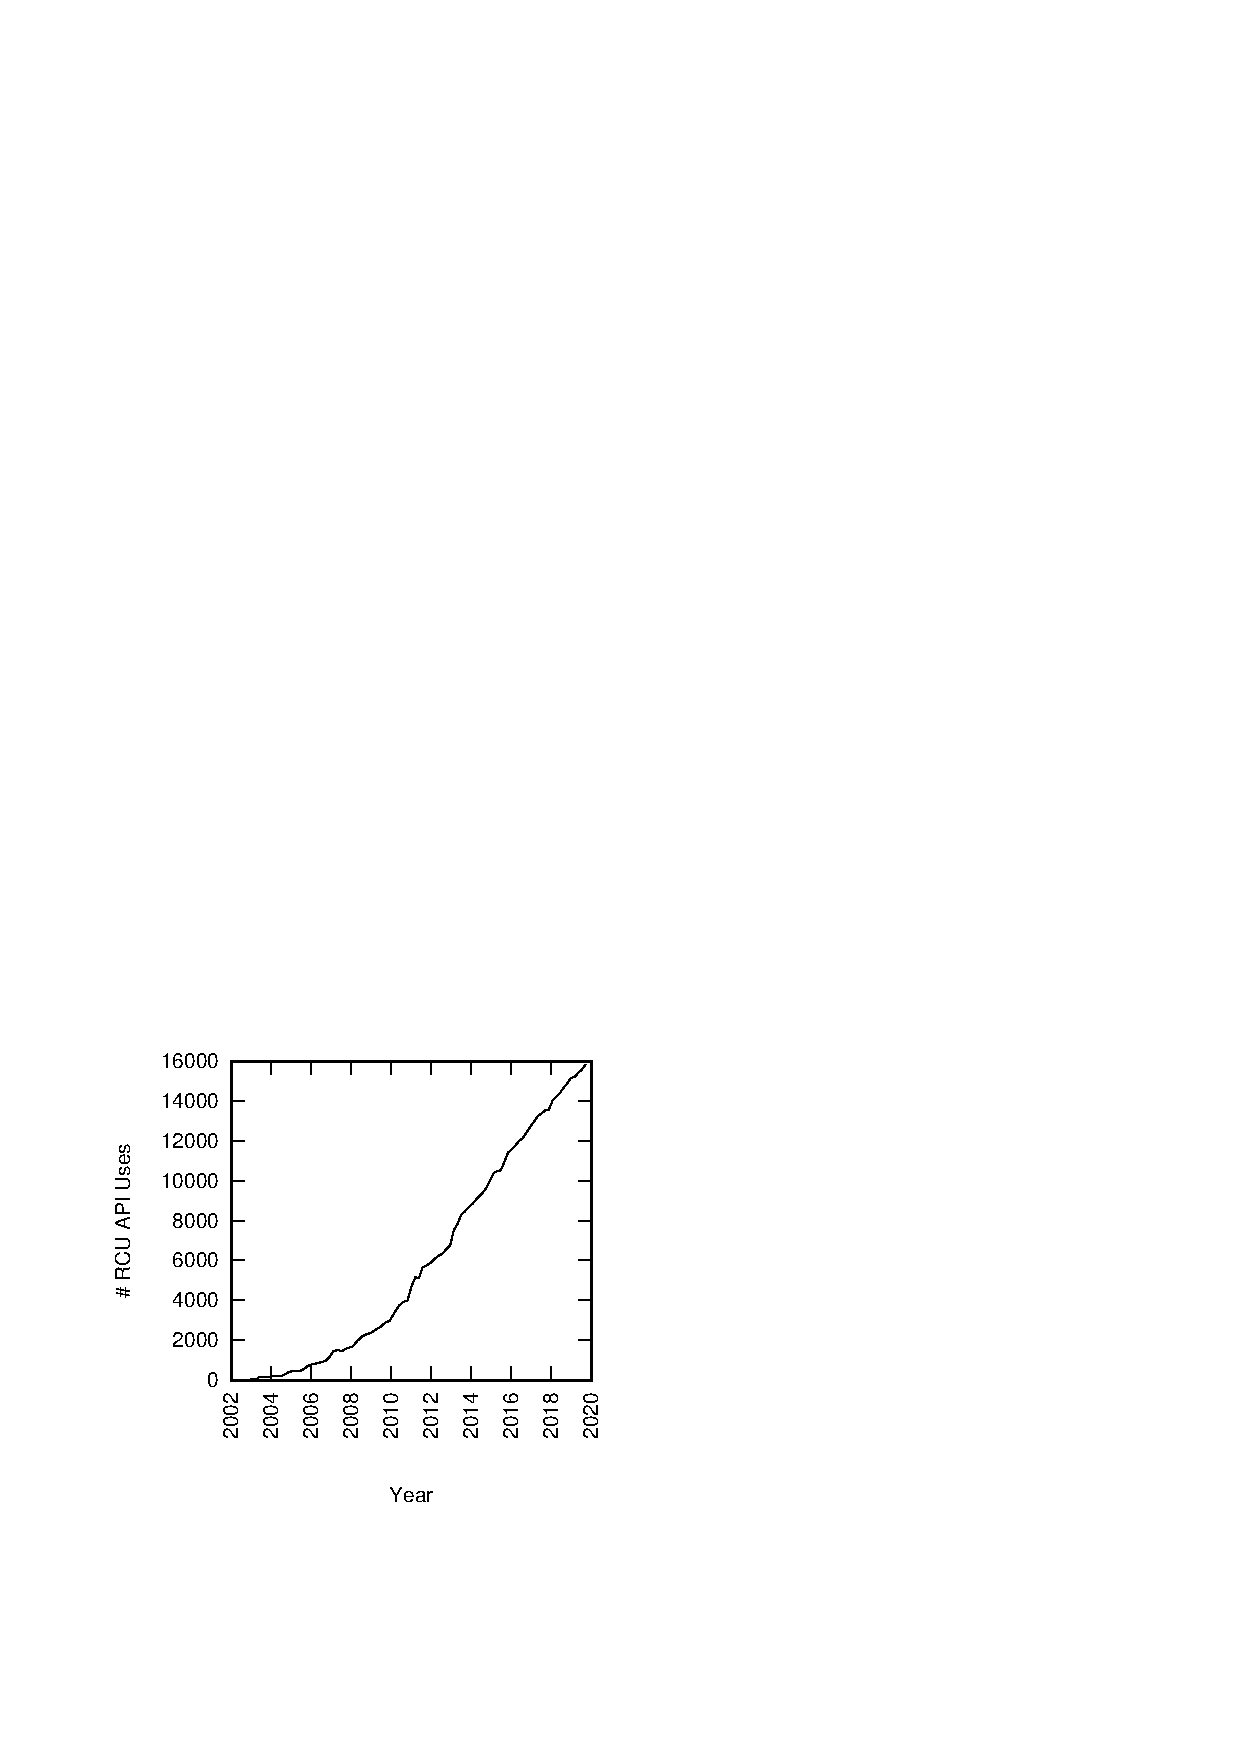
\includegraphics{defer/linux-RCU}}
\caption{RCU Usage in the Linux Kernel}
\label{fig:defer:RCU Usage in the Linux Kernel}
\end{figure}

RCU has been used in the Linux kernel since
October 2002~\cite{Torvalds2.5.43}.
Use of the RCU API has increased substantially since that time,
as can be seen in
Figure~\ref{fig:defer:RCU Usage in the Linux Kernel}.
In fact, code very similar to that in
Listing~\ref{lst:defer:Insertion and Deletion With Concurrent Readers}
is used in the Linux kernel.
RCU has enjoyed heavy use both prior to and since its acceptance
in the Linux kernel, as discussed in
\cref{sec:defer:RCU Related Work}.

It is therefore safe to say that RCU enjoys wide practical applicability.

The minimal example discussed in this section is a good introduction to RCU\@.
However, effective use of RCU often requires that you think differently
about your problem.
It is therefore useful to examine RCU's fundamentals, a task taken up
by the following section.

% defer/rcufundamental.tex

\subsection{RCU Fundamentals}
\label{sec:defer:RCU Fundamentals}
\OriginallyPublished{Section}{sec:defer:RCU Fundamentals}{RCU Fundamentals}{Linux Weekly News}{PaulEMcKenney2007WhatIsRCUFundamentally}

Authors: Paul E. McKenney and Jonathan Walpole

Read-copy update (RCU) 는 2002년 10월에 리눅스 커널에 추가된, 하나의 동기화
메커니즘입니다.
RCU 는 읽기 작업들이 업데이트 작업들과 동시에 일어날 수 있도록 함으로써 확장성
개선을 달성합니다.
기존에 일반적으로 사용되어온, 동시에 수행되는 쓰레드들에 대해 그것들이 읽기를
하는지 업데이트를 하는지와 상관없이 상호 배제를 보장하는 락킹 기능들 또는
동시의 읽기 작업은 허용하지만 업데이트가 함께 수행되는 것은 막는 reader-writer
락들과는 대조적으로 RCU 는 하나의 업데이트 쓰레드와 여러 읽기 쓰레드들 사이의
동시성을 지원합니다.
RCU 는 오브젝트들의 여러 버전들을 유지하고 그것들이 이전부터 존재해온 모든
읽기쪽 크리티컬 섹션들이 완료되기 전까지는 메모리에서 해제하지 않음으로써 읽기
작업들이 일관적임을 보장합니다.
RCU 는 오브젝트의 새 버전을 공개하고 읽는데, 그리고 예전 버전들의 정리 작업을
뒤로 미루어 한번에 처리하는데에 효과적이고 확장성 있는 메커니즘을 정의하고
사용합니다.
이런 메커니즘들은 작업을 읽기와 업데이트쪽 수행경로로 분산시키되 읽기 쪽
수행경로가 극단적으로 빠르게 하는데에 해저드 포인터와 유사한 복사와 규칙 완화를
골자로 하는 최적화 기술을 사용하지만, 읽기 쪽의 재시도는 필요 없게 합니다.
일부 경우에는 (CPU 를 뺏기지 않는 커널들), RCU 의 읽기 쪽 기능들은 아예
오버헤드가 없습니다.
\iffalse

Read-copy update (RCU) is a synchronization mechanism that was added to
the Linux kernel in October of 2002.
RCU achieves scalability
improvements by allowing reads to occur concurrently with updates.
In contrast with conventional locking primitives that ensure mutual exclusion
among concurrent threads regardless of whether they be readers or
updaters, or with reader-writer locks that allow concurrent reads but not in
the presence of updates, RCU supports concurrency between a single
updater and multiple readers.
RCU ensures that reads are coherent by
maintaining multiple versions of objects and ensuring that they are not
freed up until all pre-existing read-side critical sections complete.
RCU defines and uses efficient and scalable mechanisms for publishing
and reading new versions of an object, and also for deferring the collection
of old versions.
These mechanisms distribute the work among read and
update paths in such a way as to make read paths extremely fast, using
replication and weakening optimizations in a manner similar to
hazard pointers, but without the need for read-side retries.
In some cases (non-preemptible kernels), RCU's read-side primitives have
zero overhead.
\fi

\QuickQuiz{}
	하지만 Section~\ref{sec:defer:Sequence Locks} 의 시퀀스 락 역시 읽기
	쓰레드들과 업데이트 쓰레드들이 동시에 일을 할 수 있도록 하지 않던가요?
	\iffalse

	But doesn't Section~\ref{sec:defer:Sequence Locks}'s seqlock
	also permit readers and updaters to get work done concurrently?
	\fi
\QuickQuizAnswer{
	맞는 말이고 아닌 말이기도 합니다.
	시퀀스 락의 읽기 쓰레드들은 쓰기 쓰레드들과 동시에 수행될 수 있지만,
	이런 상황이 발생할 때마다, {\tt read\_seqretry()} 기능이 읽기 쓰레드는
	다시 수행을 시도하도록 강제할 겁니다.
	이는 시퀀스 락을 사용하명 업데이트 쓰레드와 동시에 수행되는 읽기
	쓰레드가 하는 일은 모두 취소되고 다시 수행될 것을 의미합니다.
	따라서 시퀀스 락을 사용하는 읽기 작업은 업데이트 작업과 동시에
	\emph{수행} 될 수 있지만, 이런 경우에 실제로는 어떤 일도 만들어내지
	못합니다.

	반면에, RCU 읽기 쓰레드들은 동시에 RCU 업데이트 쓰레드들이 존재하더라도
	의미있는 일을 처리해낼 수 있습니다.
	\iffalse

	Yes and no.
	Although seqlock readers can run concurrently with
	seqlock writers, whenever this happens, the {\tt read\_seqretry()}
	primitive will force the reader to retry.
	This means that any work done by a seqlock reader running concurrently
	with a seqlock updater will be discarded and redone.
	So seqlock readers can \emph{run} concurrently with updaters,
	but they cannot actually get any work done in this case.

	In contrast, RCU readers can perform useful work even in presence
	of concurrent RCU updaters.
	\fi
} \QuickQuizEnd

이는 ``RCU 는 정확히 무엇인가?'' 하는 질문과, 아마도 ``RCU 는 어떻게 동작할 수
\emph{있는가}?'' 하는 질문을 이끌어낼 수 있을 겁니다 (또는, 드물지 않게, RCU 는
동작할 수 없을 것이라는 단정을).
이 문서는 이런 질문들을 기본적 관점에서부터 다룹니다; 뒤의 일부는 RCU 를
사용법과 API 관점에서 살펴봅니다.
마지막 부분은 또한 참고할 문서 목록을 포함합니다.

RCU 는 세개의 기본적 메커니즘으로 만들어지는데, 첫번째는 항목 삽입에 사용되고,
두번째 것은 항목 삭제에, 그리고 세번째 것은 읽기 쓰레드들이 동시의 항목 추가와
삭제에 문제 없이 동작하도록 하는데 사용됩니다.
Section~\ref{sec:defer:Publish-Subscribe Mechanism}
은 항목 추가를 위한 publish-subscribe 메커니즘을 설명하고,
Section~\ref{sec:defer:Wait For Pre-Existing RCU Readers to Complete}
에서는 먼저 시작된 RCU 읽기 쓰레드들을 어떻게 기다려서 항목 삭제가 가능하게
하는지 설명하며,
Section~\ref{sec:defer:Maintain Multiple Versions of Recently Updated Objects}
에서는 최근에 업데이트된 오브젝트들의 여러 버전들을 어떻게 관리해서 동시의 항목
추가와 삭제를 가능하게 하는지 설명합니다.
마지막으로,
Section~\ref{sec:defer:Summary of RCU Fundamentals}
에서는 RCU 기본사항을 요약합니다.
\iffalse

This leads to the question ``what exactly is RCU?'', and perhaps also
to the question ``how can RCU \emph{possibly} work?'' (or, not
infrequently, the assertion that RCU cannot possibly work).
This document addresses these questions from a fundamental viewpoint;
later installments look at them from usage and from API viewpoints.
This last installment also includes a list of references.

RCU is made up of three fundamental mechanisms, the first being
used for insertion, the second being used for deletion, and the third
being used to allow readers to tolerate concurrent insertions and deletions.
Section~\ref{sec:defer:Publish-Subscribe Mechanism}
describes the publish-subscribe mechanism used for insertion,
Section~\ref{sec:defer:Wait For Pre-Existing RCU Readers to Complete}
describes how waiting for pre-existing RCU readers enabled deletion,
and
Section~\ref{sec:defer:Maintain Multiple Versions of Recently Updated Objects}
discusses how maintaining multiple versions of recently updated objects
permits concurrent insertions and deletions.
Finally,
Section~\ref{sec:defer:Summary of RCU Fundamentals}
summarizes RCU fundamentals.
\fi

\subsubsection{Publish-Subscribe Mechanism}
\label{sec:defer:Publish-Subscribe Mechanism}

\begin{figure}[tbp]
{ \scriptsize
\begin{verbatim}
  1 struct foo {
  2   int a;
  3   int b;
  4   int c;
  5 };
  6 struct foo *gp = NULL;
  7
  8 /* . . . */
  9
 10 p = kmalloc(sizeof(*p), GFP_KERNEL);
 11 p->a = 1;
 12 p->b = 2;
 13 p->c = 3;
 14 gp = p;
\end{verbatim}
}
\caption{Data Structure Publication (Unsafe)}
\label{fig:defer:Data Structure Publication (Unsafe)}
\end{figure}

RCU 의 핵심 요소 중 하나는 데이터가 동시에 수정되고 있는데도 불구하고 안전하게
그 데이터를 읽을 수 있는 능력입니다.
동시의 항목 삽입에 이런 능력을 제공하기 위해, RCU 는 공개-구독
(publish-subscribe) 메커니즘이라 생각될 수 있는 방법을 상요합니다.
예를 들어, 초기에 \co{NULL} 인 전역 포인터 \co{gp} 가 새로 할당되고 초기화된
데이터 구조체로의 포인터로 수정되려 한다고 생각해 봅시다.
Figure~\ref{fig:defer:Data Structure Publication (Unsafe)} 에 보이는 코드 조각
(추가로 적절한 락킹을 포함해서) 이 이 목적으로 사용될 수 있을 것입니다.
\iffalse

One key attribute of RCU is the ability to safely scan data, even
though that data is being modified concurrently.
To provide this ability for concurrent insertion,
RCU uses what can be thought of as a publish-subscribe mechanism.
For example, consider an initially \co{NULL} global pointer
\co{gp} that is to be modified to point to a newly allocated
and initialized data structure.
The code fragment shown in
Figure~\ref{fig:defer:Data Structure Publication (Unsafe)}
(with the addition of appropriate locking)
might be used for this purpose.
\fi

안타깝게도, 컴파일러와 CPU 가 마지막 네개의 할당문이 순서대로 수행하도록
강제하는 것이 전혀 없습니다.
\co{gp} 로의 할당이 \co{p} 필드들의 초기화 전에 일어난다면, 동시 수행중인 읽기
작업들은 이 초기화되지 않은 값들을 볼 수 있을 겁니다.
이것들이 순서를 지키도록 하기 위해 메모리 배리어들이 필요합니다만, 메모리
배리어들은 사용하기가 어렵기로 악명높습니다.
따라서 그것들을 공개 의미를 갖는 \co{rcu_assign_pointer()} 기능에 집어넣습니다.
그렇게 되면 마지막 네줄은 다음과 같이 될겁니다:
\iffalse

Unfortunately, there is nothing forcing the compiler and CPU to execute
the last four assignment statements in order.
If the assignment to \co{gp} happens before the initialization
of \co{p} fields, then concurrent readers could see the
uninitialized values.
Memory barriers are required to keep things ordered, but memory barriers
are notoriously difficult to use.
We therefore encapsulate them into a primitive
\co{rcu_assign_pointer()} that has publication semantics.
The last four lines would then be as follows:
\fi

\vspace{5pt}
\begin{minipage}[t]{\columnwidth}
\scriptsize
\begin{verbatim}
  1 p->a = 1;
  2 p->b = 2;
  3 p->c = 3;
  4 rcu_assign_pointer(gp, p);
\end{verbatim}
\end{minipage}
\vspace{5pt}

이 \co{rcu_assign_pointer()} 는 새 구조체를 \emph{공개}하고, 컴파일러와 CPU 가
\co{gp} 로의 할당이 \co{p} 로 참조되는 필드들의 할당 \emph{후에} 수행하도록
강제할 겁니다.

하지만, 업데이트 작업에 순서를 맞추는 것만으로는 충분치 않은데, 읽기 작업도
적절하게 순서가 맞춰져야 하기 때문입니다.
다음과 같은 코드 조각의 예를 생각해 봅시다:
\iffalse

The \co{rcu_assign_pointer()}
would \emph{publish} the new structure, forcing both the compiler
and the CPU to execute the assignment to \co{gp} \emph{after}
the assignments to the fields referenced by \co{p}.

However, it is not sufficient to only enforce ordering at the
updater, as the reader must enforce proper ordering as well.
Consider for example the following code fragment:
\fi

\vspace{5pt}
\begin{minipage}[t]{\columnwidth}
\scriptsize
\begin{verbatim}
  1 p = gp;
  2 if (p != NULL) {
  3   do_something_with(p->a, p->b, p->c);
  4 }
\end{verbatim}
\end{minipage}
\vspace{5pt}

이 코드 조각은 잘못된 순서에 문제가 없을 것처럼 보이지만, 안타깝게도 DEC Alpha
CPU~\cite{PaulMcKenney2005i,PaulMcKenney2005j} 와 값을 예측하는 컴파일러
최적화는, 믿든 안믿든, \co{p->a}, \co{p->b}, 그리고 \co{p->c} 가 \co{p} 의 값
전에 메모리로부터 가져와질 수 있게 할 수 있습니다.
이런 현상은 컴파일러가 \co{p} 의 값을 추측하고 \co{p->a}, \co{p->b}, 그리고
\co{p->c} 값을 가져온 후에 그 추측이 맞았는지 보기 위해 \co{p} 의 실제 값을
가져오는, 컴파일러의 값 추측 최적화의 경우에서 보기가 가장 쉬울 겁니다.
이런 종류의 최적화는 상당히 공격적이고 미친 행위 같지만, 프로파일 기반의
최적화의 문맥에서는 실제로 일어나는 일입니다.
\iffalse

Although this code fragment might well seem immune to misordering,
unfortunately, the
DEC Alpha CPU~\cite{PaulMcKenney2005i,PaulMcKenney2005j}
and value-speculation compiler optimizations can, believe it or not,
cause the values of \co{p->a}, \co{p->b}, and
\co{p->c} to be fetched before the value of \co{p}.
This is perhaps easiest to see in the case of value-speculation
compiler optimizations, where the compiler guesses the value
of \co{p} fetches \co{p->a}, \co{p->b}, and
\co{p->c} then fetches the actual value of \co{p}
in order to check whether its guess was correct.
This sort of optimization is quite aggressive, perhaps insanely so,
but does actually occur in the context of profile-driven optimization.
\fi

분명히, 우리는 컴파일러와 CPU 로부터 이런 종류의 야바위질을 막아야 합니다.
\co{rcu_dereference()} 기능은 이런 목적을 위해 필요한 어떤 메모리 배리어
인스트럭션과 컴파일러 지시어들을 사용합니다:\footnote{
	리눅스 커널에서, \co{rcu_dereference()} 는 volatile 캐스팅으로
	구현되고, DEC Alpha 에서는 메모리 배리어 인스트럭션으로 구현됩니다.
	C11 과 C++11 표준에서는 \co{memory_order_consume} 이
	\co{rcu_dereference()} 지원을 제공하기 위한 의도로 만들어졌습니다만,
	이를 native로 구현한 컴파일러는 아직 없습니다.
	(컴파일러들은 대신 \co{memory_order_consume} 을
	\co{memory_order_acuire} 로 강화시켜서, 약한 순서 규칙의 시스템에서는
	필요없는 메모리 배리어 인스트럭션을 만듭니다.)}
\iffalse

Clearly, we need to prevent this sort of skullduggery on the
part of both the compiler and the CPU.
The \co{rcu_dereference()} primitive uses
whatever memory-barrier instructions and compiler
directives are required for this purpose:\footnote{
	In the Linux kernel, \co{rcu_dereference()} is implemented via
	a volatile cast, and, on DEC Alpha, a memory barrier instruction.
	In the C11 and C++11 standards, \co{memory_order_consume}
	is intended to provide longer-term support for \co{rcu_dereference()},
	but no compilers implement this natively yet.
	(They instead strengthen \co{memory_order_consume} to
	\co{memory_order_acquire}, thus emitting a needless memory-barrier
	instruction on weakly ordered systems.)}
\fi

\vspace{5pt}
\begin{minipage}[t]{\columnwidth}
\scriptsize
\begin{verbatim}
  1 rcu_read_lock();
  2 p = rcu_dereference(gp);
  3 if (p != NULL) {
  4   do_something_with(p->a, p->b, p->c);
  5 }
  6 rcu_read_unlock();
\end{verbatim}
\end{minipage}
\vspace{5pt}

따라서 \co{rcu_dereference()} 함수는 특정 포인터로 주어지는 값에 대한
\emph{구독} 으로, 뒤따르는 dereference 오퍼레이션들은 해당 포인터를 공개한,
연관된 \co{rcu_assign_pointer()} 오퍼레이션 전에 발생한 초기화 작업의 결과들을
보게 될 것이 보장된다고 이해될 수 있습니다.
\co{rcu_read_lock()} 과 \co{rcu_read_unlock()} 함수 호출들은 반드시 필요합니다:
이것들은 RCU read-side 크리티컬 섹션을 정의합니다.
이것들의 목적인
Section~\ref{sec:defer:Wait For Pre-Existing RCU Readers to Complete} 에서
설명됩니다만, 이것들은 결코 스피닝하거나 블락킹 하지 않고, \co{list_add_rcu()}
가 동시에 수행되는 것을 막지도 않습니다.
사실, \co{CONFIG_PREEMPT} 옵션이 켜져있지 않은 커널에서 이것들은 아무 코드도
생성하지 않습니다.
\iffalse

The \co{rcu_dereference()} primitive can thus be thought of
as \emph{subscribing} to a given value of the specified pointer,
guaranteeing that subsequent dereference operations will see any
initialization that occurred before the corresponding
\co{rcu_assign_pointer()} operation that published that pointer.
The \co{rcu_read_lock()} and \co{rcu_read_unlock()}
calls are absolutely required: they define the extent of the
RCU read-side critical section.
Their purpose is explained in
Section~\ref{sec:defer:Wait For Pre-Existing RCU Readers to Complete},
however, they never spin or block, nor do they prevent the
\co{list_add_rcu()} from executing concurrently.
In fact, in non-\co{CONFIG_PREEMPT} kernels, they generate
absolutely no code.
\fi

\begin{figure}[tb]
\begin{center}
\resizebox{3in}{!}{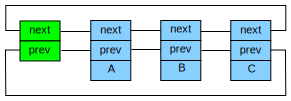
\includegraphics{defer/Linux_list}}
\end{center}
\caption{Linux Circular Linked List}
\label{fig:defer:Linux Circular Linked List}
\end{figure}

\begin{figure}[tb]
\begin{center}
\resizebox{3in}{!}{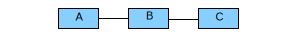
\includegraphics{defer/Linux_list_abbr}}
\end{center}
\caption{Linux Linked List Abbreviated}
\label{fig:defer:Linux Linked List Abbreviated}
\end{figure}

이론상으로는 \co{rcu_assign_pointer()} 와 \co{rcu_dereference()} 는 상상할 수
있는 RCU 로 보호되는 데이터 구조는 얼마든지 만들 수 있지만, 실제로는
고차원의 방법을 사용하는게 나은 경우가 많이 있습니다.
그런 이유로, \co{rcu_assign_pointer()} 와 \co{rcu_dereference()} 함수들이
리눅스에 있는 리스트 조정 API 의 특별한 RCU 사용 버전에 내장되어 있습니다.
리눅스는 이중 링크드 리스트의 두가지 버전을 가지고 있는데, 순환 형태의 {\tt
struct list\_head} 와 선형의 {\tt struct hlist\_head}/{\tt struct hlist\_node}
쌍입니다.
앞의 버전은
Figure~\ref{fig:defer:Linux Circular Linked List} 에 그려져 있는데, (왼쪽의)
초록 상자는 리스트 헤더를 나타내고 (오른쪽의 세개의) 파란 박스들은 리스트의
원소들을 의미합니다.
이 방법은 다루기가 힘들기 때문에
Figure~\ref{fig:defer:Linux Linked List Abbreviated} 에 보인 것처럼 헤더 없이
(파란) 원소들만을 보이는 형태로 간략화해서 나타낼 수 있습니다.
\iffalse

Although \co{rcu_assign_pointer()} and
\co{rcu_dereference()} can in theory be used to construct any
conceivable RCU-protected data structure, in practice it is often better
to use higher-level constructs.
Therefore, the \co{rcu_assign_pointer()} and
\co{rcu_dereference()}
primitives have been embedded in special RCU variants of Linux's
list-manipulation API.
Linux has two variants of doubly linked list, the circular
{\tt struct list\_head} and the linear
{\tt struct hlist\_head}/{\tt struct hlist\_node} pair.
The former is laid out as shown in
Figure~\ref{fig:defer:Linux Circular Linked List},
where the green (leftmost) boxes represent the list header and the blue
(rightmost three) boxes represent the elements in the list.
This notation is cumbersome, and will therefore be abbreviated as shown in
Figure~\ref{fig:defer:Linux Linked List Abbreviated},
which shows only the non-header (blue) elements.
\fi

\begin{figure}[tbp]
{ \scriptsize
\begin{verbatim}
  1 struct foo {
  2   struct list_head *list;
  3   int a;
  4   int b;
  5   int c;
  6 };
  7 LIST_HEAD(head);
  8
  9 /* . . . */
 10
 11 p = kmalloc(sizeof(*p), GFP_KERNEL);
 12 p->a = 1;
 13 p->b = 2;
 14 p->c = 3;
 15 list_add_rcu(&p->list, &head);
\end{verbatim}
}
\caption{RCU Data Structure Publication}
\label{fig:defer:RCU Data Structure Publication}
\end{figure}

이 링크드 리스트에 포인터 공개 예제의 기법을 적용하는 것은
Figure~\ref{fig:defer:RCU Data Structure Publication} 에 보여진 코드와 같은
형태로 귀결될 겁니다.

Line~15 는 여러개의 \co{list_add_rcu()} 가 동시에 수행되는 것을 막기 위해 어떤
다른 동기화 메커니즘 (가장 흔하게는 어떤 종류의 락) 을 사용해야만 합니다.
하지만, 그런 동기화는 이 \co{list_add()} 의 수행을 RCU 읽기 작업들과 동시에
수행되는 것을 못하게 하지는 않습니다.

RCU 로 보호되는 리스트를 구독하는 행위는 간단합니다:
\iffalse

Adapting the pointer-publish example for the linked list results in
the code shown in
Figure~\ref{fig:defer:RCU Data Structure Publication}.

Line~15 must be protected by some synchronization mechanism (most
commonly some sort of lock) to prevent multiple \co{list_add_rcu()}
instances from executing concurrently.
However, such synchronization does not prevent this \co{list_add()}
instance from executing concurrently with RCU readers.

Subscribing to an RCU-protected list is straightforward:
\fi

\vspace{5pt}
\begin{minipage}[t]{\columnwidth}
\scriptsize
\begin{verbatim}
  1 rcu_read_lock();
  2 list_for_each_entry_rcu(p, head, list) {
  3   do_something_with(p->a, p->b, p->c);
  4 }
  5 rcu_read_unlock();
\end{verbatim}
\end{minipage}
\vspace{5pt}

앞의 \co{list_add_rcu()} 함수는 원소를 공개하고, 특정 리스트의 헤드에 집어넣고,
이에 연관된 \co{list_for_each_entry_rcu()} 호출이 정상적으로 같은 원소를
구독하게 될것을 보장합니다.
\iffalse

The \co{list_add_rcu()} primitive publishes an entry, inserting it at
the head of the specified list, guaranteeing that the corresponding
\co{list_for_each_entry_rcu()} invocation will properly subscribe to
this same entry.
\fi

\QuickQuiz{}
	{\tt list\_add\_rcu()} 와 정확히 똑같은 시간에
	{\tt list\_for\_each\_entry\_rcu()} 이 수행되면 segfault 가 날 수 있을
	것 같은데, 이걸 무엇이 방지해 주나요?
	\iffalse

	What prevents the {\tt list\_for\_each\_entry\_rcu()} from
	getting a segfault if it happens to execute at exactly the same
	time as the {\tt list\_add\_rcu()}?
	\fi
\QuickQuizAnswer{
	리눅스가 돌아가는 모든 시스템에서 포인터로의 로드와 스토어는 모두
	어토믹한데, 즉, 포인터로의 스토어가 같은 포인터로부터의 로드와 같은
	시점에 일어난다면, 이 로드는 초기값이나 저장된 값을 가져오지, 그 두
	값이 섞여진 값을 가져오는 일은 결코 없습니다.
	또한, {\tt list\_for\_each\_entry\_rcu()} 는 항상 리스트를 앞으로만
	움직이지, 결코 뒤로 움직이지는 않습니다.
	따라서, {\tt list\_for\_each\_entry\_rcu()} 는 {\tt list\_add\_rc()} 를
	통해 들어온 원소를 보거나 보지 않을 뿐이지만 어떤 경우든 적합하게 잘
	형성된 리스트를 볼 겁니다.
	\iffalse

	On all systems running Linux, loads from and stores
	to pointers are atomic, that is, if a store to a pointer occurs at
	the same time as a load from that same pointer, the load will return
	either the initial value or the value stored, never some bitwise
	mashup of the two.
	In addition, the {\tt list\_for\_each\_entry\_rcu()} always proceeds
	forward through the list, never looking back.
	Therefore, the {\tt list\_for\_each\_entry\_rcu()} will either see
	the element being added by {\tt list\_add\_rcu()} or it will not,
	but either way, it will see a valid well-formed list.
	\fi
} \QuickQuizEnd

\begin{figure}[tb]
\begin{center}
\resizebox{3in}{!}{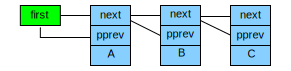
\includegraphics{defer/Linux_hlist}}
\end{center}
\caption{Linux Linear Linked List}
\label{fig:defer:Linux Linear Linked List}
\end{figure}

리눅스의 다른 이중 링크드 리스트인 hlist 는 선형 리스트인데, 이는 헤더로의
포인터만이 필요하지
Figure~\ref{fig:defer:Linux Linear Linked List} 에 보여진 순환 형태의
리스트처럼 두개의 포인터가 필요하진 않습니다.
따라서, hlist 의 사용은 해시 버킷 배열들이나 커다란 해시 테이블에서는 메모리
사용량을 반으로 줄일 수 있습니다.
앞에서와 같이, 이 형태는 다루기가 까다로우므로, hlist 들은
Figure~\ref{fig:defer:Linux Linked List Abbreviated} 에 보인 것과 같은 형태로
간략화 될 겁니다.
\iffalse

Linux's other doubly linked list, the hlist,
is a linear list, which means that
it needs only one pointer for the header rather than the two
required for the circular list, as shown in
Figure~\ref{fig:defer:Linux Linear Linked List}.
Thus, use of hlist can halve the memory consumption for the hash-bucket
arrays of large hash tables.
As before, this notation is cumbersome, so hlists will be abbreviated
in the same way lists are, as shown in
Figure~\ref{fig:defer:Linux Linked List Abbreviated}.
\fi

\begin{figure}[tbp]
{ \scriptsize
\begin{verbatim}
  1 struct foo {
  2   struct hlist_node *list;
  3   int a;
  4   int b;
  5   int c;
  6 };
  7 HLIST_HEAD(head);
  8
  9 /* . . . */
 10
 11 p = kmalloc(sizeof(*p), GFP_KERNEL);
 12 p->a = 1;
 13 p->b = 2;
 14 p->c = 3;
 15 hlist_add_head_rcu(&p->list, &head);
\end{verbatim}
}
\caption{RCU {\tt hlist} Publication}
\label{fig:defer:RCU hlist Publication}
\end{figure}

새로운 원소를 RCU 로 보호되는 hlist 에 공개하는 건
as shown in Figure~\ref{fig:defer:RCU hlist Publication} 에 보여진 것처럼,
순환형 리스트에서 했던 것과 상당히 유사합니다.

앞에서와 같이, line~15 는 예를 들면 락과 같은, 어떤 종류의 동기화 메커니즘으로
보호되어야만 합니다.

RCU 로 보호되는 hlist 를 구독하는 행위 역시 순환형 리스트에서와 비슷합니다:
\iffalse

Publishing a new element to an RCU-protected hlist is quite similar
to doing so for the circular list,
as shown in Figure~\ref{fig:defer:RCU hlist Publication}.

As before, line~15 must be protected by some sort of synchronization
mechanism, for example, a lock.

Subscribing to an RCU-protected hlist is also similar to the
circular list:
\fi

\vspace{5pt}
\begin{minipage}[t]{\columnwidth}
\scriptsize
\begin{verbatim}
  1 rcu_read_lock();
  2 hlist_for_each_entry_rcu(p, q, head, list) {
  3   do_something_with(p->a, p->b, p->c);
  4 }
  5 rcu_read_unlock();
\end{verbatim}
\end{minipage}
\vspace{5pt}

\QuickQuiz{}
	{\tt list\_for\_each\_entry\_rcu()} 에서는 한개면 되었던 포인터가 왜
	{\tt hlist\_for\_each\_entry\_rcu()} 에서는 두개나 넘겨줘야 하는거죠?
	\iffalse

	Why do we need to pass two pointers into
	{\tt hlist\_for\_each\_entry\_rcu()}
	when only one is needed for {\tt list\_for\_each\_entry\_rcu()}?
	\fi
\QuickQuizAnswer{
	hlist 에서는 헤드를 만나는 대신에 NULL 체크를 할 필요가 있기
	때문입니다.
	(하나의 포인터만 사용하는 {\tt hlist\_for\_each\_entry\_rcu()} 를
	한번 구현해 보세요.
	만약 좋은 해결책을 찾는다면, 정말 좋은 일일 겁니다!)
	\iffalse

	Because in an hlist it is necessary to check for
	NULL rather than for encountering the head.
	(Try coding up a single-pointer {\tt hlist\_for\_each\_entry\_rcu()}.
	If you come up with a nice solution, it would be a very good thing!)
	\fi
} \QuickQuizEnd

\begin{table*}[tb]
\begin{center}
\scriptsize
\begin{tabular}{l||l|l|l}
Category  & Publish	& Retract	& Subscribe \\
\hline
\hline
Pointers  & \co{rcu_assign_pointer()}
			& \co{rcu_assign_pointer(..., NULL)}~~
					& \co{rcu_dereference()} \\
\hline
Lists     & \parbox{1.5in}{
		\co{list_add_rcu()} \\
		\co{list_add_tail_rcu()} \\
		\co{list_replace_rcu()} }
			& \co{list_del_rcu()}
					& \co{list_for_each_entry_rcu()}~~~ \\
\hline
Hlists    & \parbox{1.5in}{
		\co{hlist_add_after_rcu()} \\
		\co{hlist_add_before_rcu()}  \\
		\co{hlist_add_head_rcu()} \\
		\co{hlist_replace_rcu()} }
			& \co{hlist_del_rcu()}
					& \co{hlist_for_each_entry_rcu()}~~~~~
\end{tabular}
\end{center}
\caption{RCU Publish and Subscribe Primitives}
\label{tab:defer:RCU Publish and Subscribe Primitives}
\end{table*}

RCU 공개와 구독 기능들의 집합이
Table~\ref{tab:defer:RCU Publish and Subscribe Primitives} 에 ``구독취소'' 또는
철회를 위한 추가적인 기능들과 함께 표시 되어 있습니다.

\co{list_replace_rcu()}, \co{list_del_rcu()},
\co{hlist_replace_rcu()}, and \co{hlist_del_rcu()}
API 들이 복잡도를 더함을 알아두세요.
교체되거나 삭제된 데이터 원소를 메모리에서 해제하는데 안전한 시점은 언제일까요?
자세히 들어가서, 모든 읽기 작업들이 특정 데이터 원소로의 레퍼런스들을
해제한 시점을 어떻게 하면 알 수 있을까요?

이 질문들은 다음의 섹션에서 다루어집니다.
\iffalse

The set of RCU publish and subscribe primitives are shown in
Table~\ref{tab:defer:RCU Publish and Subscribe Primitives},
along with additional primitives to ``unpublish'', or retract.

Note that the \co{list_replace_rcu()}, \co{list_del_rcu()},
\co{hlist_replace_rcu()}, and \co{hlist_del_rcu()}
APIs add a complication.
When is it safe to free up the data element that was replaced or
removed?
In particular, how can we possibly know when all the readers
have released their references to that data element?

These questions are addressed in the following section.
\fi

\subsubsection{Wait For Pre-Existing RCU Readers to Complete}
\label{sec:defer:Wait For Pre-Existing RCU Readers to Complete}

In its most basic form, RCU is a way of waiting for things to finish.
Of course, there are a great many other ways of waiting for things to
finish, including reference counts, reader-writer locks, events, and so on.
The great advantage of RCU is that it can wait for each of
(say) 20,000 different things without having to explicitly
track each and every one of them, and without having to worry about
the performance degradation, scalability limitations, complex deadlock
scenarios, and memory-leak hazards that are inherent in schemes
using explicit tracking.

In RCU's case, the things waited on are called
``RCU read-side critical sections''.
An RCU read-side critical section starts with an
\co{rcu_read_lock()} primitive, and ends with a corresponding
\co{rcu_read_unlock()} primitive.
RCU read-side critical sections can be nested, and may contain pretty
much any code, as long as that code does not explicitly block or sleep
(although a special form of RCU called SRCU~\cite{PaulEMcKenney2006c}
does permit general sleeping in SRCU read-side critical sections).
If you abide by these conventions, you can use RCU to wait for \emph{any}
desired piece of code to complete.

RCU accomplishes this feat by indirectly determining when these
other things have finished~\cite{PaulEMcKenney2007whatisRCU,
PaulEMcKenney2007PreemptibleRCU}.

\begin{figure}[tb]
\begin{center}
\resizebox{3in}{!}{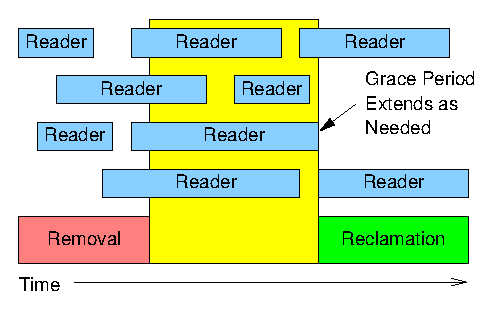
\includegraphics{defer/GracePeriodGood}}
\end{center}
\caption{Readers and RCU Grace Period}
\label{fig:defer:Readers and RCU Grace Period}
\end{figure}

In particular, as shown in
Figure~\ref{fig:defer:Readers and RCU Grace Period},
RCU is a way of
waiting for pre-existing RCU read-side critical sections to completely
finish, including memory operations executed by those critical sections.
However, note that RCU read-side critical sections
that begin after the beginning
of a given grace period can and will extend beyond the end of that grace
period.

The following pseudocode shows the basic form of algorithms that use
RCU to wait for readers:

\begin{enumerate}
\item	Make a change, for example, replace an element in a linked list.
\item	Wait for all pre-existing RCU read-side critical sections to
	completely finish (for example, by using the
	\co{synchronize_rcu()} primitive).
	The key observation here is that subsequent RCU read-side critical
	sections have no way to gain a reference to the newly removed
	element.
\item	Clean up, for example, free the element that was replaced above.
\end{enumerate}

\begin{figure}[tbp]
{ \scriptsize
\begin{verbatim}
  1 struct foo {
  2   struct list_head *list;
  3   int a;
  4   int b;
  5   int c;
  6 };
  7 LIST_HEAD(head);
  8
  9 /* . . . */
 10
 11 p = search(head, key);
 12 if (p == NULL) {
 13   /* Take appropriate action, unlock, & return. */
 14 }
 15 q = kmalloc(sizeof(*p), GFP_KERNEL);
 16 *q = *p;
 17 q->b = 2;
 18 q->c = 3;
 19 list_replace_rcu(&p->list, &q->list);
 20 synchronize_rcu();
 21 kfree(p);
\end{verbatim}
}
\caption{Canonical RCU Replacement Example}
\label{fig:defer:Canonical RCU Replacement Example}
\end{figure}

The code fragment shown in
Figure~\ref{fig:defer:Canonical RCU Replacement Example},
adapted from those in Section~\ref{sec:defer:Publish-Subscribe Mechanism},
demonstrates this process, with field \co{a} being the search key.

Lines~19, 20, and 21 implement the three steps called out above.
Lines~16-19 gives RCU (``read-copy update'') its name: while permitting
concurrent \emph{reads}, line~16 \emph{copies} and lines~17-19
do an \emph{update}.

As discussed in Section~\ref{sec:defer:Introduction to RCU},
the \co{synchronize_rcu()} primitive can be quite simple
(see Section~\ref{sec:defer:``Toy'' RCU Implementations}
for additional ``toy'' RCU implementations).
However, production-quality implementations must deal with
difficult corner cases and also incorporate
powerful optimizations, both of which result in significant complexity.
Although it is good to know that there is a simple conceptual
implementation of \co{synchronize_rcu()}, other questions remain.
For example, what exactly do RCU
readers see when traversing a concurrently updated list?
This question is addressed in the following section.

\subsubsection{Maintain Multiple Versions of Recently Updated Objects}
\label{sec:defer:Maintain Multiple Versions of Recently Updated Objects}

This section demonstrates how RCU maintains multiple versions of
lists to accommodate synchronization-free readers.
Two examples are presented showing how an element
that might be referenced by a given reader must remain intact
while that reader remains in its RCU read-side critical section.
The first example demonstrates deletion of a list element,
and the second example demonstrates replacement of an element.

\paragraph{Example 1: Maintaining Multiple Versions During Deletion}
\label{sec:defer:Example 1: Maintaining Multiple Versions During Deletion}

We can now revisit the deletion example from
Section~\ref{sec:defer:Introduction to RCU},
but now with the benefit of a firm understanding of the fundamental
concepts underlying RCU.
To begin this new version of the deletion example,
we will modify lines~11-21 in
Figure~\ref{fig:defer:Canonical RCU Replacement Example}
to read as follows:

\vspace{5pt}
\begin{minipage}[t]{\columnwidth}
\scriptsize
\begin{verbatim}
  1 p = search(head, key);
  2 if (p != NULL) {
  3   list_del_rcu(&p->list);
  4   synchronize_rcu();
  5   kfree(p);
  6 }
\end{verbatim}
\end{minipage}
\vspace{5pt}

\begin{figure}[tb]
\begin{center}
\resizebox{3in}{!}{\includegraphics{defer/RCUDeletion}}
\end{center}
\caption{RCU Deletion From Linked List}
\label{fig:defer:RCU Deletion From Linked List}
\end{figure}

This code will update the list as shown in
Figure~\ref{fig:defer:RCU Deletion From Linked List}.
The triples in each element represent the values of fields \co{a},
\co{b}, and \co{c}, respectively.
The red-shaded elements
indicate that RCU readers might be holding references to them,
so in the initial state at the top of the diagram, all elements
are shaded red.
Please note that
we have omitted the backwards pointers and the link from the tail
of the list to the head for clarity.

After the \co{list_del_rcu()} on
line~3 has completed, the \co{5,6,7}~element
has been removed from the list, as shown in the second row of
Figure~\ref{fig:defer:RCU Deletion From Linked List}.
Since readers do not synchronize directly with updaters,
readers might be concurrently scanning this list.
These concurrent readers might or might not see the newly removed element,
depending on timing.
However, readers that were delayed (e.g., due to interrupts, ECC memory
errors, or, in \co{CONFIG_PREEMPT_RT} kernels, preemption)
just after fetching a pointer to the newly removed element might
see the old version of the list for quite some time after the
removal.
Therefore, we now have two versions of the list, one with element
\co{5,6,7} and one without.
The \co{5,6,7}~element in the second row of the figure is now
shaded yellow, indicating
that old readers might still be referencing it, but that new
readers cannot obtain a reference to it.

Please note that readers are not permitted to maintain references to
element~\co{5,6,7} after exiting from their RCU read-side
critical sections.
Therefore,
once the \co{synchronize_rcu()} on
line~4 completes, so that all pre-existing readers are
guaranteed to have completed,
there can be no more readers referencing this
element, as indicated by its green shading on the third row of
Figure~\ref{fig:defer:RCU Deletion From Linked List}.
We are thus back to a single version of the list.

At this point, the \co{5,6,7}~element may safely be
freed, as shown on the final row of
Figure~\ref{fig:defer:RCU Deletion From Linked List}.
At this point, we have completed the deletion of
element~\co{5,6,7}.
The following section covers replacement.

\paragraph{Example 2: Maintaining Multiple Versions During Replacement}
\label{sec:defer:Example 2: Maintaining Multiple Versions During Replacement}

To start the replacement example,
here are the last few lines of the
example shown in
Figure~\ref{fig:defer:Canonical RCU Replacement Example}:

\vspace{5pt}
\begin{minipage}[t]{\columnwidth}
\scriptsize
\begin{verbatim}
  1 q = kmalloc(sizeof(*p), GFP_KERNEL);
  2 *q = *p;
  3 q->b = 2;
  4 q->c = 3;
  5 list_replace_rcu(&p->list, &q->list);
  6 synchronize_rcu();
  7 kfree(p);
\end{verbatim}
\end{minipage}
\vspace{5pt}

\begin{figure}[tbp]
\begin{center}
\resizebox{2.7in}{!}{\includegraphics{defer/RCUReplacement}}
\end{center}
\caption{RCU Replacement in Linked List}
\label{fig:defer:RCU Replacement in Linked List}
\end{figure}

The initial state of the list, including the pointer \co{p},
is the same as for the deletion example, as shown on the
first row of
Figure~\ref{fig:defer:RCU Replacement in Linked List}.

As before,
the triples in each element represent the values of fields \co{a},
\co{b}, and \co{c}, respectively.
The red-shaded elements might be referenced by readers,
and because readers do not synchronize directly with updaters,
readers might run concurrently with this entire replacement process.
Please note that
we again omit the backwards pointers and the link from the tail
of the list to the head for clarity.

The following text describes how to replace the \co{5,6,7} element
with \co{5,2,3} in such a way that any given reader sees one of these
two values.

Line~1 \co{kmalloc()}s a replacement element, as follows,
resulting in the state as shown in the second row of
Figure~\ref{fig:defer:RCU Replacement in Linked List}.
At this point, no reader can hold a reference to the newly allocated
element (as indicated by its green shading), and it is uninitialized
(as indicated by the question marks).

Line~2 copies the old element to the new one, resulting in the
state as shown in the third row of
Figure~\ref{fig:defer:RCU Replacement in Linked List}.
The newly allocated element still cannot be referenced by readers, but
it is now initialized.

Line~3 updates \co{q->b} to the value ``2'', and
line~4 updates \co{q->c} to the value ``3'', as shown on the fourth row of
Figure~\ref{fig:defer:RCU Replacement in Linked List}.

Now, line~5 does the replacement, so that the new element is
finally visible to readers, and hence is shaded red, as shown on
the fifth row of
Figure~\ref{fig:defer:RCU Replacement in Linked List}.
At this point, as shown below, we have two versions of the list.
Pre-existing readers might see the \co{5,6,7} element (which is
therefore now shaded yellow), but
new readers will instead see the \co{5,2,3} element.
But any given reader is guaranteed to see some well-defined list.

After the \co{synchronize_rcu()} on line~6 returns,
a grace period will have elapsed, and so all reads that started before the
\co{list_replace_rcu()} will have completed.
In particular, any readers that might have been holding references
to the \co{5,6,7} element are guaranteed to have exited
their RCU read-side critical sections, and are thus prohibited from
continuing to hold a reference.
Therefore, there can no longer be any readers holding references
to the old element, as indicated its green shading in the sixth row of
Figure~\ref{fig:defer:RCU Replacement in Linked List}.
As far as the readers are concerned, we are back to having a single version
of the list, but with the new element in place of the old.

After the \co{kfree()} on line 7 completes, the list will
appear as shown on the final row of
Figure~\ref{fig:defer:RCU Replacement in Linked List}.

Despite the fact that RCU was named after the replacement case,
the vast majority of RCU usage within the Linux kernel relies on
the simple deletion case shown in
Section~\ref{sec:defer:Maintain Multiple Versions of Recently Updated Objects}.

\paragraph{Discussion}
\label{sec:defer:Discussion}

These examples assumed that a mutex was held across the entire
update operation, which would mean that there could be at most two
versions of the list active at a given time.

\QuickQuiz{}
	How would you modify the deletion example to permit more than two
	versions of the list to be active?
\QuickQuizAnswer{
	One way of accomplishing this is as shown in
	Figure~\ref{fig:defer:Concurrent RCU Deletion}.

\begin{figure}[htbp]
{ \centering
\begin{verbatim}
  1 spin_lock(&mylock);
  2 p = search(head, key);
  3 if (p == NULL)
  4   spin_unlock(&mylock);
  5 else {
  6   list_del_rcu(&p->list);
  7   spin_unlock(&mylock);
  8   synchronize_rcu();
  9   kfree(p);
 10 }
\end{verbatim}
}
\caption{Concurrent RCU Deletion}
\label{fig:defer:Concurrent RCU Deletion}
\end{figure}

	Note that this means that multiple concurrent deletions might be
	waiting in \co{synchronize_rcu()}.
} \QuickQuizEnd

\QuickQuiz{}
	How many RCU versions of a given list can be
	active at any given time?
\QuickQuizAnswer{
	That depends on the synchronization design.
	If a semaphore protecting the update is held across the grace period,
	then there can be at most two versions, the old and the new.

	However, suppose that only the search, the update, and the
	\co{list_replace_rcu()} were protected by a lock, so that
	the \co{synchronize_rcu()} was outside of that lock, similar
	to the code shown in
	Figure~\ref{fig:defer:Concurrent RCU Deletion}.
	Suppose further that a large number of threads undertook an
	RCU replacement at about the same time, and that readers
	are also constantly traversing the data structure.

	Then the following sequence of events could occur, starting from
	the end state of
	Figure~\ref{fig:defer:RCU Replacement in Linked List}:

	\begin{enumerate}
	\item	Thread~A traverses the list, obtaining a reference to
		the 5,2,3 element.
	\item	Thread~B replaces the 5,2,3 element with a new
		5,2,4 element, then waits for its \co{synchronize_rcu()}
		call to return.
	\item	Thread~C traverses the list, obtaining a reference to
		the 5,2,4 element.
	\item	Thread~D replaces the 5,2,4 element with a new
		5,2,5 element, then waits for its \co{synchronize_rcu()}
		call to return.
	\item	Thread~E traverses the list, obtaining a reference to
		the 5,2,5 element.
	\item	Thread~F replaces the 5,2,5 element with a new
		5,2,6 element, then waits for its \co{synchronize_rcu()}
		call to return.
	\item	Thread~G traverses the list, obtaining a reference to
		the 5,2,6 element.
	\item	And the previous two steps repeat quickly, so that all
		of them happen before any of the \co{synchronize_rcu()}
		calls return.
	\end{enumerate}

	Thus, there can be an arbitrary number of versions active,
	limited only by memory and by how many updates could be completed
	within a grace period.
	But please note that data structures that are updated so frequently
	probably are not good candidates for RCU.
	That said, RCU can handle high update rates when necessary.
} \QuickQuizEnd

This sequence of events shows how RCU updates use multiple versions
to safely carry out changes in presence of concurrent readers.
Of course, some algorithms cannot gracefully handle multiple versions.
There are techniques
for adapting such algorithms to RCU~\cite{PaulEdwardMcKenneyPhD},
but these are beyond the scope of this section.

\subsubsection{Summary of RCU Fundamentals}
\label{sec:defer:Summary of RCU Fundamentals}

This section has described the three fundamental components of RCU-based
algorithms:

\begin{enumerate}
\item	a publish-subscribe mechanism for adding new data,

\item	a way of waiting for pre-existing RCU readers to finish, and

\item	a discipline of maintaining multiple versions to permit
	change without harming or unduly delaying concurrent RCU readers.
\end{enumerate}

\QuickQuiz{}
	How can RCU updaters possibly delay RCU readers, given that the
	{\tt rcu\_read\_lock()} and {\tt rcu\_read\_unlock()}
	primitives neither spin nor block?
\QuickQuizAnswer{
	The modifications undertaken by a given RCU updater will cause the
	corresponding CPU to invalidate cache lines containing the data,
	forcing the CPUs running concurrent RCU readers to incur expensive
	cache misses.
	(Can you design an algorithm that changes a data structure
	\emph{without}
	inflicting expensive cache misses on concurrent readers?
	On subsequent readers?)
} \QuickQuizEnd

These three RCU components
allow data to be updated in face of concurrent readers, and
can be combined in different ways to
implement a surprising variety of different types of RCU-based algorithms,
some of which are described in the following section.

% defer/rcuAPI.tex

\subsection{RCU Linux-Kernel API}
\label{sec:defer:RCU Linux-Kernel API}
\OriginallyPublished{Section}{sec:defer:RCU Linux-Kernel API}{RCU Linux-Kernel API}{Linux Weekly News}{PaulEMcKenney2008WhatIsRCUAPI}

이 섹션은 RCU를 그것의 리눅스 커널 API의 관점에서 바라봅니다.
Section~\ref{sec:defer:RCU has a Family of Wait-to-Finish APIs}
은 RCU 의 wait-to-finish API들을, 그리고
Section~\ref{sec:defer:RCU has Publish-Subscribe and Version-Maintenance APIs}
에서는 RCU 의 publish-subscribe 와 version-maintenance API 들을 소개합니다.
마지막으로,
Section~\ref{sec:defer:So, What is RCU Really?}
에서는 결론을 정리합니다.
\iffalse

This section looks at RCU from the viewpoint of its Linux-kernel API.
Section~\ref{sec:defer:RCU has a Family of Wait-to-Finish APIs}
presents RCU's wait-to-finish APIs, and
Section~\ref{sec:defer:RCU has Publish-Subscribe and Version-Maintenance APIs}
presents RCU's publish-subscribe and version-maintenance APIs.
Finally,
Section~\ref{sec:defer:So, What is RCU Really?}
presents concluding remarks.
\fi

\subsubsection{RCU has a Family of Wait-to-Finish APIs}
\label{sec:defer:RCU has a Family of Wait-to-Finish APIs}

\begin{sidewaystable*}[htbp]
\centering
\scriptsize\tymin=1.4in
\begin{tabulary}{7.8in}{L|L|L|L|L|L}
Attribute &
    RCU Classic &
	RCU BH &
	    RCU Sched &
		Realtime RCU &
		    SRCU \\
\hline
\hline
Purpose &
    Original &
	Prevent DDoS attacks &
	    Wait for preempt-disable regions, hardirqs, \& NMIs &
	        Realtime response &
		    Sleeping readers \\
\hline
Availability &
    2.5.43 &
	2.6.9 &
	    2.6.12 &
		2.6.26 &
		    2.6.19 \\
\hline
Read-side primitives &
    \begin{minipage}[t]{1.4in}{ \raggedright
      \co{rcu_read_lock()}~! \\
      \co{rcu_read_unlock()}~! }\end{minipage} &
	\begin{minipage}[t]{1.4in}{ \raggedright
	  \co{rcu_read_lock_bh()} \\
	  \co{rcu_read_unlock_bh()} }\end{minipage} &
	    \begin{minipage}[t]{1.4in}{ \raggedright
	      \co{preempt_disable()} \\
	      \co{preempt_enable()} \\
	      (and friends) }\end{minipage} &
	        \begin{minipage}[t]{1.4in}{ \raggedright
		  \co{rcu_read_lock()} \\
		  \co{rcu_read_unlock()} }\end{minipage} &
		    \begin{minipage}[t]{1.4in}{ \raggedright
		      \co{srcu_read_lock()} \\
		      \co{srcu_read_unlock()} }\end{minipage} \\
\hline
{ Update-side primitives (synchronous) } &
    { \co{synchronize_rcu()} \co{synchronize_net()} } &
	\co{synchronize_rcu_bh()} &
	    \co{synchronize_sched()} &
	        { \co{synchronize_rcu()} \co{synchronize_net()} } &
		    \co{synchronize_srcu()} \\
\hline
{ Update-side primitives (asynchronous/callback) } &
    \co{call_rcu()} ! &
	\co{call_rcu_bh()} &
	    \co{call_rcu_sched()} &
	        \co{call_rcu()} &
		    \co{call_srcu()} \\
\hline
{ Update-side primitives (wait for callbacks) } &
    \co{rcu_barrier()} &
	\co{rcu_barrier_bh()} &
	    \co{rcu_barrier_sched()} &
	        \co{rcu_barrier()} &
		    N/A \\
\hline
Type-safe memory &
    \co{SLAB_DESTROY_BY_RCU} &
	&
	    &
	        \co{SLAB_DESTROY_BY_RCU} &
		    \\
\hline
Read side constraints &
    No blocking &
	No bottom-half (BH) enabling &
	    No blocking &
	        Only preemption and lock acquisition &
		    No \co{synchronize_srcu()} wtih same \co{srcu_struct} \\
\hline
Read side overhead &
    Preempt disable/enable (free on non-PREEMPT) &
	BH disable/enable &
	    Preempt disable/enable (free on non-PREEMPT) &
	        Simple instructions, irq disable/enable &
		    Simple instructions, preempt disable/enable, memory barriers \\
\hline
Asynchronous update-side overhead &
    sub-microsecond &
	sub-microsecond &
	    sub-microsecond &
	        sub-microsecond &
		    N/A \\
\hline
Grace-period latency &
    10s of milliseconds &
	10s of milliseconds &
	    10s of milliseconds &
	        10s of milliseconds &
		    10s of milliseconds \\
\hline
Non-\co{PREEMPT_RT} implementation &
    RCU Classic &
	RCU BH &
	    RCU Classic &
	        Preemptible RCU &
		    SRCU \\
\hline
\co{PREEMPT_RT} implementation &
    Preemptible RCU &
	Realtime RCU &
	    Forced Schedule on all CPUs &
	        Realtime RCU &
		    SRCU \\
\end{tabulary}
\caption{RCU Wait-to-Finish APIs}
\label{tab:defer:RCU Wait-to-Finish APIs}
\end{sidewaystable*}

``RCU 는 무엇인가'' 에 대한 가장 직접적인 답변은 RCU 는 리눅스 커널에서
사용되는 API 라는 것으로, 각각 잠들 수 없는 버전과 잠들 수 있는 버전 API 들의
RCU 읽기 쓰레드 기다리기 부분을 보이는
Table~\ref{tab:defer:RCU Wait-to-Finish APIs},
그리고 그 API 의 publish-subscribe 부분을 보이는
Table~\ref{tab:defer:RCU Publish-Subscribe and Version Maintenance APIs} 에
요약되어 있습니다.
\iffalse

The most straightforward answer to ``what is RCU'' is that RCU is
an API used in the Linux kernel, as summarized by
Table~\ref{tab:defer:RCU Wait-to-Finish APIs},
which shows the wait-for-RCU-readers portions of the non-sleepable and
sleepable APIs, respectively,
and by
Table~\ref{tab:defer:RCU Publish-Subscribe and Version Maintenance APIs},
which shows the publish-subscribe portions of the API.
\fi

RCU 가 처음이라면
Table~\ref{tab:defer:RCU Wait-to-Finish APIs} 의 행들 중 하나에만 집중해 볼
것을 고려해 볼만 한데, 각각의 행은 리눅스 커널의 RCU API 패밀리 중 하나의
멤버를 요약하고 있습니다.
예를 들어, 리눅스 커널에서 RCU 가 어떻게 사용되는지를 이해하고자 하는게 주된
목표라면, ``RCU Classic'' 가장 자주 사용되므로 여기서부터 시작하는게 좋을
것입니다.
반면에, 자신의 이익을 위해 RCU 를 이해하고자 한다면 ``SRCU'' 가 가장 간단한 API
를 제공합니다.
나중에도 언제든 다른 행을 볼 수 있습니다.

이미 RCU 에 친숙하다면, 이 표들은 유용한 레퍼런스로 사용될 수 있을 겁니다.
\iffalse

If you are new to RCU, you might consider focusing on just one
of the columns in
Table~\ref{tab:defer:RCU Wait-to-Finish APIs},
each of which summarizes one member of the Linux kernel's RCU API family.
For example, if you are primarily interested in understanding how RCU
is used in the Linux kernel, ``RCU Classic'' would be the place to start,
as it is used most frequently.
On the other hand, if you want to understand RCU for its own sake,
``SRCU'' has the simplest API.
You can always come back for the other columns later.

If you are already familiar with RCU, these tables can
serve as a useful reference.
\fi

\QuickQuiz{}
	Table~\ref{tab:defer:RCU Wait-to-Finish APIs} 의 일부 셀들은 왜 느낌표
	(``!'') 를 가지고 있나요?
	\iffalse

	Why do some of the cells in
	Table~\ref{tab:defer:RCU Wait-to-Finish APIs}
	have exclamation marks (``!'')?
	\fi
\QuickQuizAnswer{
	느낌표와 함께 표시된 API 멤버들 (\co{rcu_read_lock()},
	\co{rcu_read_unlock()}, 그리고 \co{call_rcu()}) 만이 과거 90년대 중반에
	Paul E. McKenney 가 신경썼던 리눅스 RCU API 의 멤버들입니다.
	이 시절에는, 그는 그가 RCU 에 대해 알아야 할 것들을 모두 알고 있다는
	잘못된 인상을 가지고 있었습니다.
	\iffalse

	The API members with exclamation marks (\co{rcu_read_lock()},
	\co{rcu_read_unlock()}, and \co{call_rcu()}) were the
	only members of the Linux RCU API that Paul E. McKenney was aware
	of back in the mid-90s.
	During this timeframe, he was under the mistaken impression that
	he knew all that there is to know about RCU.
	\fi
} \QuickQuizEnd

이 ``RCU Classic'' 행은 RCU read-side 크리티컬 섹션들은 \co{rcu_read_lock()} 과
\co{rcu_read_unlock()} 으로 구분지어지고 중첩될수도 있는, 최초의 RCU 구현에
해당합니다.
여기에 연관되는 동기적인 업데이트 쪽 기능들인 \co{synchronize_rcu()} 와 그것과
같은 의미인 \co{synchronize_net()} 은 동시에 실행중인 RCU read-side 크리티컬
섹션들이 모두 완료되기를 기다립니다.
이 기다림의 길이는 ``grace period'' 라고 알려져 있습니다.
비동기적인 업데이트 쪽 기능인 \co{call_rcu()} 는 뒤따르는 grace period 후에
특정 함수를 특정 인자와 함께 호출해 줍니다.
예를 들어, \co{call_rcu(p,f);} 는 다음의 grace period 후에 ``RCU callback''
\co{f(p)} 의 호출이 이뤄지게 합니다.
\co{call_rcu()} 를 사용하는 리눅스 커널 모듈을 언로딩 한다던가 해서 모든 RCU
callback 들이 완료되기를 기다려야만 하는 상황도
존재합니다~\cite{PaulEMcKenney2007rcubarrier}.
\co{rcu_barrier()} 기능이 그 일을 합니다.
더 최신의 계층적 RCU~\cite{PaulEMcKenney2008HierarchicalRCU} 구현 또한 ``RCU
Classic'' 시맨틱을 고수함을 알아두세요.
\iffalse

The ``RCU Classic'' column corresponds to the original RCU implementation,
in which RCU read-side critical sections are delimited by
\co{rcu_read_lock()} and \co{rcu_read_unlock()}, which
may be nested.
The corresponding synchronous update-side primitives,
\co{synchronize_rcu()}, along with its synonym
\co{synchronize_net()}, wait for any currently executing
RCU read-side critical sections to complete.
The length of this wait is known as a ``grace period''.
The asynchronous update-side primitive, \co{call_rcu()},
invokes a specified function with a specified argument after a
subsequent grace period.
For example, \co{call_rcu(p,f);} will result in
the ``RCU callback'' \co{f(p)}
being invoked after a subsequent grace period.
There are situations,
such as when unloading a Linux-kernel module that uses \co{call_rcu()},
when it is necessary to wait for all
outstanding RCU callbacks to complete~\cite{PaulEMcKenney2007rcubarrier}.
The \co{rcu_barrier()} primitive does this job.
Note that the more recent hierarchical
RCU~\cite{PaulEMcKenney2008HierarchicalRCU}
implementation also adheres to ``RCU Classic'' semantics.
\fi

마지막으로, RCU 는
Section~\ref{sec:defer:RCU is a Way of Providing Type-Safe Memory} 에서 설명한
것처럼 type-safe 메모리~\cite{Cheriton96a} 를 제공하는데 사용될 수도 있습니다.
RCU 의 문맥에서, type-safe 메모리는 주어진 데이터 원소가 그것에 접근하는 모든
RCU read-side 크리티컬 섹션 사이에서 그 타입이 바뀌지 않는다는 것을 보장합니다.
RCU 기반의 type-safe 메모리를 사용하기 위해서는 \co{SLAB_DESTROY_BY_RCU} 를
\co{kmem_cache_create()} 에 넘겨야 합니다.
\co{SLAB_DESTROY_BY_RCU} 는 \co{kmem_cache_alloc()} 이 \co{kmem_cache_free()}
로 자유가 된 메모리를 즉시 재할당 하는 것을 막는 일은 \emph{결코} 하지 않음을
알아두는 게 중요합니다!
사실, \co{rcu_dereference} 로 리턴된, \co{SLAB_DESTROY_RCU} 로 보호되는 데이터
구조체는 상당히 여러번 메모리 해제되고 재할당 될 수 있는데, 심지어
\co{rcu_read_lock()} 으로 보호되고 있을 때도 그러합니다.
대신, \co{SLAB_DESTROY_BY_RCU} 는 RCU grace period 가 끝나기 전까지는
\co{kmem_cache_free()} 가 완전히 해제된 데이터 구조체들의 slab 을 시스템에
반납하는 것을 방지해 줍니다.
짧게 말해서, 비록 데이터 원소가 굉장히 자주 해제되고 재할당될 수 있지만, 최소한
그것의 타입은 똑같이 남아있을 겁니다.
\iffalse

Finally, RCU may be used to provide
type-safe memory~\cite{Cheriton96a}, as described in
Section~\ref{sec:defer:RCU is a Way of Providing Type-Safe Memory}.
In the context of RCU, type-safe memory guarantees that a given
data element will not change type during any RCU read-side critical section
that accesses it.
To make use of RCU-based type-safe memory, pass
\co{SLAB_DESTROY_BY_RCU} to
\co{kmem_cache_create()}.
It is important to note that \co{SLAB_DESTROY_BY_RCU} will
\emph{in no way}
prevent \co{kmem_cache_alloc()} from immediately reallocating
memory that was just now freed via \co{kmem_cache_free()}!
In fact, the \co{SLAB_DESTROY_BY_RCU}-protected data structure
just returned by \co{rcu_dereference} might be freed and reallocated
an arbitrarily large number of times, even when under the protection
of \co{rcu_read_lock()}.
Instead, \co{SLAB_DESTROY_BY_RCU} operates by preventing
\co{kmem_cache_free()}
from returning a completely freed-up slab of data structures
to the system until after an RCU grace period elapses.
In short, although the data element might be freed and reallocated arbitrarily
often, at least its type will remain the same.
\fi

\QuickQuiz{}
	많은 수의 RCU read-side 크리티컬 섹션들이 \co{synchronize_rcu()} 실행을
	무기한 블록시키는 걸 어떻게 막을 수 있나요?
	\iffalse

	How do you prevent a huge number of RCU read-side critical
	sections from indefinitely blocking a \co{synchronize_rcu()}
	invocation?
	\fi
\QuickQuizAnswer{
	RCU read-side 크리티컬 섹션들이 \co{synchronize_rcu()} 실행을 무기한
	블록하는걸 막을 필요가 전혀 없는데, \co{synchronize_rcu()} 실행은
	\emph{전부터 존재한} RCU read-side 크리티컬 섹션들만 기다리면 되기
	때문입니다.
	따라서 각 RCU read-side 크리티컬 섹션이 한정된 길이를 갖는다면, 아무
	문제가 없습니다.
	\iffalse

	There is no need to do anything to prevent RCU read-side
	critical sections from indefinitely blocking a
	\co{synchronize_rcu()} invocation, because the
	\co{synchronize_rcu()} invocation need wait only for
	\emph{pre-existing} RCU read-side critical sections.
	So as long as each RCU read-side critical section is
	of finite duration, there should be no problem.
	\fi
} \QuickQuizEnd

\QuickQuiz{}
	\co{synchronize_rcu()} API 는 전부터 존재한 인터럽트 핸들러들이 모두
	완료되길 기다리죠, 맞죠?
	\iffalse

	The \co{synchronize_rcu()} API waits for all pre-existing
	interrupt handlers to complete, right?
	\fi
\QuickQuizAnswer{
	전혀 그렇지 않아요!
	그리고 preemption 가능한 RCU 를 사용하고 있다면 특히나 그렇지 않습니다!
	대안으로, \co{rcu_read_lock()} 과 \co{rcu_read_unlock()} 를
	\co{synchronize_rcu()} 기다리기를 바라는 인터럽트 핸들러 안에 위치시킬
	수 있겠습니다.
	\iffalse

	Absolutely not!
	And especially not when using preemptible RCU!
	You instead want \co{synchronize_irq()}.
	Alternatively, you can place calls to \co{rcu_read_lock()}
	and \co{rcu_read_unlock()} in the specific interrupt handlers that
	you want \co{synchronize_rcu()} to wait for.
	\fi
} \QuickQuizEnd

``RCU BH'' 행에서, \co{rcu_read_lock_bh()} 와 \co{rcu_read_unlock_bh()} 는
크리티컬 섹션을 구분짓고, \co{synchronize_rcu_bh()} 는 하나의 grace period 를
기다리며, \co{call_rcu_bh()} 는 다음 grace period 후에 특정 함수를 특정 인자와
함께 호출해 줍니다.
\iffalse

In the ``RCU BH'' column, \co{rcu_read_lock_bh()} and
\co{rcu_read_unlock_bh()} delimit RCU read-side critical
sections, \co{synchronize_rcu_bh()} waits for a grace period,
and \co{call_rcu_bh()} invokes the specified
function and argument after a later grace period.
\fi

\QuickQuiz{}
	이것들을 섞어서 활용하면 어떻게 되나요?
	예를 들어, \co{rcu_read_lock()} 과 \co{rcu_read_unlock()} 을 RCU
	read-side 크리티컬 섹션을 구분하는데 사용하지만 \co{call_rcu_bh()} 를
	RCU callback 을 위해 사용한다고 하면요?
	\iffalse

	What happens if you mix and match?
	For example, suppose you use \co{rcu_read_lock()} and
	\co{rcu_read_unlock()} to delimit RCU read-side critical
	sections, but then use \co{call_rcu_bh()} to post an
	RCU callback?
	\fi
\QuickQuizAnswer{
	\co{call_rcu_bh()} 가 실행되는 시점에 \co{rcu_read_lock_bh()} 와
	\co{rcu_read_unlock_bh()} 로 구분된 RCU read-side 크리티컬 섹션들이
	존재하지 않는다면 RCU 는 이 콜백을 곧바로 수행해도 되는 권한을 갖게
	되어서, 해당 RCU read-side 크리티컬 섹션이 사용중인 데이터 구조체를
	메모리에서 해제해버릴 수도 있습니다!
	이건 단순히 이론적인 가능성이 아닙니다: \co{rcu_read_lock()} 과
	\co{rcu_read_unlock()} 으로 구분지어졌고 오랫동안 동작중인 RCU
	read-side 크리티컬 섹션은 이런 실패에 취약합니다.

	하지만, \co{rcu_dereference()} 함수들은 모든 RCU 변종들에 적용됩니다.
	(변종별 \co{rcu_dereference()} 를 만들려는 시도도 있었지만, 그건 너무
	혼란스러웠습니다.)
	\iffalse

	If there happened to be no RCU read-side critical
	sections delimited by \co{rcu_read_lock_bh()} and
	\co{rcu_read_unlock_bh()} at the time \co{call_rcu_bh()}
	was invoked, RCU would be within its rights to invoke the callback
	immediately, possibly freeing a data structure still being used by
	the RCU read-side critical section!
	This is not merely a theoretical possibility: a long-running RCU
	read-side critical section delimited by \co{rcu_read_lock()}
	and \co{rcu_read_unlock()} is vulnerable to this failure mode.

	However, the \co{rcu_dereference()} family of functions apply
	to all flavors of RCU.
	(There was an attempt to have per-flavor variants of
	\co{rcu_dereference()}, but it was just too messy.)
	\fi
} \QuickQuizEnd

\QuickQuiz{}
	하드웨어 인터럽트 핸들러들은 묵시적인 \co{rcu_read_lock_bh()} 의 보호
	아래 있다고 생각되어도 되겠죠?
	\iffalse

	Hardware interrupt handlers can be thought of as being
	under the protection of an implicit \co{rcu_read_lock_bh()},
	right?
	\fi
\QuickQuizAnswer{
	전혀 그렇지 않아요!
	그리고 preemption 가능한 RCU 를 사용중일 때에는 특히나 그렇지 않습니다!
	``rcu\_bh'' 로 보호되는 데이터 구조체를 인터럽트 핸들러 내에서 접근하려
	한다면, 명시적으로 \co{rcu_read_lock_bh()} 와 \co{rcu_read_unlock_bh()}
	를 사용해야 합니다.
	\iffalse

	Absolutely not!
	And especially not when using preemptible RCU!
	If you need to access ``rcu\_bh''-protected data structures
	in an interrupt handler, you need to provide explicit calls to
	\co{rcu_read_lock_bh()} and \co{rcu_read_unlock_bh()}.
	\fi
} \QuickQuizEnd

``RCU Sched'' 행에서, preemption 을 불가능하게 하는 모든 동작은 RCU read-side
크리티컬 섹션처럼 동작되고, \co{synchronize_sched()} 는 연관된 RCU grace period
를 기다립니다.
이 RCU API 패밀리는 2.6.12 커널에서 들어왔는데, 이것이 과거의
\co{synchronize_kernel()} API 를 (RCU Classic 을 위한) 지금의
\co{synchronize_rcu()} 와 (RCU Sched 를 위한) \co{synchronize_sched()} 로
나눴습니다.
RCU Sched 는 처음부터 비동기적인 \co{call_rcu_sched()} 인터페이스를 가지고 있진
않았다가 2.6.26 에서 추가되었음을 알아두세요.
리눅스 커뮤니티의 어떤 의미에서의 minimalist 철학에 의해, API 들은 필요한
경우에 기반해서 추가됩니다.
\iffalse

In the ``RCU Sched'' column, anything that disables preemption
acts as an RCU read-side critical section, and \co{synchronize_sched()}
waits for the corresponding RCU grace period.
This RCU API family was added in the 2.6.12 kernel, which split the
old \co{synchronize_kernel()} API into the current
\co{synchronize_rcu()} (for RCU Classic) and
\co{synchronize_sched()} (for RCU Sched).
Note that RCU Sched did not originally have an asynchronous
\co{call_rcu_sched()} interface, but one was added in 2.6.26.
In accordance with the quasi-minimalist philosophy of the Linux
community, APIs are added on an as-needed basis.
\fi

\QuickQuiz{}
	RCU Classic 과 RCU Sched 를 섞어서 사용하면 어떻게 되나요?
	\iffalse

	What happens if you mix and match RCU Classic and RCU Sched?
	\fi
\QuickQuizAnswer{
	Non-\co{PREEMPT} 나 \co{PREEMPT} 커널에서는 이 두개의 일은 우연히
	섞이게 되는데, 그런 커널 빌드에서 RCU Classic 과 RCU Sched 는 같은
	구현으로 매핑되기 때문입니다.
	하지만, 이런 조합은 -rt 패치셋을 사용하는 \co{PREEMPT_RT} 빌드에서는
	치명적인데 Realtime RCU 의 read-side 크리티컬 섹션들은 preemption 당할
	수 있어서 \co{synchronize_sched()} 가 RCU read-side 크리티컬 섹션이
	\co{rcu_read_unlock()} 호출을 하기 전에 리턴할 수 있기 때문입니다.
	이는 데이터 구조체가 그 구조체를 사용하는 read-side 크리티컬 섹션이
	끝나기 전에 메모리 해제될 수 있게 해서 커널의 보험 통계적 리스크를 무척
	증가시킬 수 있습니다.

	실제로, RCU Classic 과 RCU Sched 의 분리는 preemption 가능해야 하는 RCU
	read-side 크리티컬 섹션들로부터 영감을 받았습니다.
	\iffalse

	In a non-\co{PREEMPT} or a \co{PREEMPT} kernel, mixing these
	two works ``by accident'' because in those kernel builds, RCU Classic
	and RCU Sched map to the same implementation.
	However, this mixture is fatal in \co{PREEMPT_RT} builds using the -rt
	patchset, due to the fact that Realtime RCU's read-side critical
	sections can be preempted, which would permit
	\co{synchronize_sched()} to return before the
	RCU read-side critical section reached its \co{rcu_read_unlock()}
	call.
	This could in turn result in a data structure being freed before the
	read-side critical section was finished with it,
	which could in turn greatly increase the actuarial risk experienced
	by your kernel.

	In fact, the split between RCU Classic and RCU Sched was inspired
	by the need for preemptible RCU read-side critical sections.
	\fi
} \QuickQuizEnd

\QuickQuiz{}
	일반적으로, 모든 전부터 존재한 인터럽트 핸들러들을 기다리는데에
	\co{synchronize_sched()} 에 의존해선 안됩니다, 맞죠?
	\iffalse

	In general, you cannot rely on \co{synchronize_sched()} to
	wait for all pre-existing interrupt handlers,
	right?
	\fi
\QuickQuizAnswer{
	맞습니다!
	-rt 리눅스는 쓰레드로 도는 인터럽트 핸들러들을 사용하기 때문에,
	인터럽트 핸들러 내부에서의 컨텍스트 스위치가 있을 수 있습니다.
	\co{synchronize_sched()} 는 각 CPU 가 컨텍스트 스위치를 할 때까지만
	기다리기 때문에, 특정 인터럽트 핸들러가 완료되기 전에 리턴을 할수도
	있습니다.

	특정 인터럽트 핸들러가 완료되기까지 기다려야 한다면, 그대신
	\co{synchronize_irq()} 를 사용하거나 명시적으로 RCU read-side 크리티컬
	섹션들을 기다리기 원하는 인터럽트 핸들러들 안에 위치시켜야 합니다.
	\iffalse

	That is correct!
	Because -rt Linux uses threaded interrupt handlers, there can
	be context switches in the middle of an interrupt handler.
	Because \co{synchronize_sched()} waits only until each
	CPU has passed through a context switch, it can return
	before a given interrupt handler completes.

	If you need to wait for a given interrupt handler to complete,
	you should instead use \co{synchronize_irq()} or place
	explicit RCU read-side critical sections in the interrupt
	handlers that you wish to wait on.
	\fi
} \QuickQuizEnd

``Realtime RCU'' 행은 RCU Classic 과 똑같은 API 를 가지고 있는데, 차이점은 RCU
read-side 크리티컬 섹션들이 preemption 당할 수 있고 spinlock 을 획득하는 사이
블락될 수 있다는 점 뿐입니다.
Realtime RCU 의 설계는 다른곳에도 설명되어
있습니다~\cite{PaulEMcKenney2007PreemptibleRCU}.
\iffalse

The ``Realtime RCU'' column has the same API as does
RCU Classic, the only difference being that RCU read-side critical
sections may be preempted and may block while acquiring spinlocks.
The design of Realtime RCU is described
elsewhere~\cite{PaulEMcKenney2007PreemptibleRCU}.
\fi

Table~\ref{tab:defer:RCU Wait-to-Finish APIs} 의 ``SRCU'' 행은 RCU
read-side 크리티컬 섹션들 안에서 일반적인 잠들기를 허용하는 특수한 RCU API 를
보입니다~\cite{PaulEMcKenney2006c}.
물론, SRCU read-side 크리티컬 섹션 안에서의 \co{synchronize_srcu()} 사용은
스스로의 deadlock 을 유발할 수 있으므로, 반드시 피해져야 합니다.
SRCU 의 앞의 RCU 구현들과의 차이점은 각각의 별개의 SRCU 사용처마다 호출자가
\co{srcu_struct} 를 할당해야 한다는 겁니다.
이 방법은 SRCU read-side 크리티컬 섹션들이 연관되지 않은
\co{synchronize_srcu()} 실행을 블록하는 것을 방지합니다.
또한, 이 RCU 변종에서는 \co{srcu_read_lock()} 이 연관된 \co{srcu_read_unlock()}
에 전달되어야 하는 값을 리턴합니다.
\iffalse

The ``SRCU'' column in
Table~\ref{tab:defer:RCU Wait-to-Finish APIs}
displays a specialized RCU API that permits
general sleeping in RCU read-side critical
sections~\cite{PaulEMcKenney2006c}.
Of course,
use of \co{synchronize_srcu()} in an SRCU read-side
critical section can result in
self-deadlock, so should be avoided.
SRCU differs from earlier RCU implementations in that the caller
allocates an \co{srcu_struct} for each distinct SRCU
usage.
This approach prevents SRCU read-side critical sections from blocking
unrelated \co{synchronize_srcu()} invocations.
In addition, in this variant of RCU, \co{srcu_read_lock()}
returns a value that must be passed into the corresponding
\co{srcu_read_unlock()}.
\fi

\QuickQuiz{}
	\co{call_srcu()} 사용에 있어 조심해야 하는 이유는 무엇일까요?
	\iffalse

	Why should you be careful with \co{call_srcu()}?
	\fi
\QuickQuizAnswer{
	하나의 테스크는 SRC 콜백들을 매우 빠르게 등록할 수 있습니다.
	SRCU 가 읽기 쓰레드들이 임의의 기간동안 블록될 수 있도록 허용함을
	생각하면, 이는 임의의 커다란 양의 메모리를 소모할 것을 알 수 있습니다.
	반대로, 동기적인 \co{synchronize_srcu()} 인터페이스에서는 주어진
	태스크는 다음 grace period 를 기다리는 걸 시작하기 전에 주어진 grace
	period 를 기다리는 것을 마무리 해야만 합니다.
	\iffalse

	A single task could register SRCU callbacks very quickly.
	Given that SRCU allows readers to block for arbitrary periods of
	time, this could consume an arbitrarily large quantity of memory.
	In contrast, given the synchronous \co{synchronize_srcu()}
	interface, a given task must finish waiting for a given grace period
	before it can start waiting for the next one.
	\fi
} \QuickQuizEnd

\QuickQuiz{}
	어떤 조건에서 \co{synchronize_srcu()} 가 SRCU read-side 크리티컬 섹션
	내에서 안전하게 사용될 수 있을까요?
	\iffalse

	Under what conditions can \co{synchronize_srcu()} be safely
	used within an SRCU read-side critical section?
	\fi
\QuickQuizAnswer{
	원론적으로, 특정 \co{srcu_struct} 와 함께, \co{synchronize_srcu()} 는
	어떤 다른 \co{srcu_struct} 를 사용하는 SRCU read-side 크리티컬 섹션
	안에서 사용될 수 있습니다.
	하지만, 실제에서는 이런 짓을 하는건 거의 분명하게 나쁜 생각입니다.
	세부적으로는
	Figure~\ref{fig:defer:Multistage SRCU Deadlocks} 에 보인 코드가 여전히
	데드락을 일으킬 수 있을 것입니다.
	\iffalse

	In principle, you can use
	\co{synchronize_srcu()} with a given \co{srcu_struct}
	within an SRCU read-side critical section that uses some other
	\co{srcu_struct}.
	In practice, however, doing this is almost certainly a bad idea.
	In particular, the code shown in
	Figure~\ref{fig:defer:Multistage SRCU Deadlocks}
	could still result in deadlock.
	\fi

{
\begin{verbbox}
  1 idx = srcu_read_lock(&ssa);
  2 synchronize_srcu(&ssb);
  3 srcu_read_unlock(&ssa, idx);
  4
  5 /* . . . */
  6
  7 idx = srcu_read_lock(&ssb);
  8 synchronize_srcu(&ssa);
  9 srcu_read_unlock(&ssb, idx);
\end{verbbox}
}
\begin{figure}[htbp]
\centering
\theverbbox
\caption{Multistage SRCU Deadlocks}
\label{fig:defer:Multistage SRCU Deadlocks}
\end{figure}
%
} \QuickQuizEnd

리눅스 커널은 분명히 놀랍도록 많은 RCU API 와 구현을 가지고 있습니다.
이 수를 줄이려는 희망이 있는데, 리눅스 커널의 특정 빌드는 현재 세개의 API 들
뒤에 최대 네개의 구현들을 가지고 있다는 사실 (RCU Classic 과 Realtime RCU 는
같은 API 를 공유합니다) 이 그 증거입니다.
하지만, 충분한 조사와 분석이 필요할텐데, 많은 락킹 API 들 가운데 하나를
제거하려면 필요한 것처럼 말입니다.

이 다양한 RCU API 들은 RCU read-side 크리티컬 섹션들이 반드시 제공해야 하는
forward-progress 보장사항으로 차별화 되고 그 범위로도 차별화되는데, 다음과
같습니다:
\iffalse

The Linux kernel currently has a surprising number of RCU APIs and
implementations.
There is some hope of reducing this number, evidenced by the fact
that a given build of the Linux kernel currently has at most
four implementations behind three APIs (given that RCU Classic
and Realtime RCU share the same API).
However, careful inspection and analysis will be required, just as
would be required in order to eliminate one of the many locking APIs.

The various RCU APIs are distinguished by the forward-progress
guarantees that their RCU read-side critical sections must provide,
and also by their scope, as follows:
\fi

\begin{enumerate}
\item	RCU BH: read-side 크리티컬 섹션들은 NMI 와 인터럽트 핸들러들을 제외한
	모든 것에 대해 forward progress 를 보장해야만 합니다만
	software-interrupt (\co{softirq}) 핸들러들은 제외입니다.
	RCU BH 는 범위내에서 글로벌 합니다.
\item	RCU Sched: read-side 크리티컬 섹션들은 NMI 와 \co{softirq} 핸들러들을
	포함한 irq 핸들러들을 제외한 모든것들에 forward progress 를 보장해야
	합니다.
	RCU Sched 는 범위내에서 글로벌합니다.
\item	RCU (Classic 과 Real-time 둘 다): read-side 크리티컬 섹션들은 NMI
	핸들러, irq 핸들러, \co{softirq} 핸들러, 그리고 (real-time 의 경우) 더
	높은 우선순위의 real-time task 를 제외한 모든 것에 forward progress 를
	보장해야 합니다.
	RCU 는 범위내에서 글로벌합니다.
\item	SRCU: read-side 크리티컬 섹션들은 다른 태스크가 연관된 grace
	period 가 완료되기를 기다리고 있지 않다면 forward progress 를 보장하지
	않아도 됩니다. 이런 상황에서 이 read-side 크리티컬 섹션들은 수초
	이내에는 완료되어야 합니다 (그리고 더 빠르면 더 좋습니다).\footnote{
		단순히 forward-progress guarantee 가 없다고 말하는 대신 이런
		명확한 설명을 하도록 재촉해준 James Bottomley 에게 감사의
		말씀을 드립니다.}
	SRCU 의 범위는 각각 연관된 \co{srcu_struct} 의 사용에 따라 정의됩니다.
\iffalse

\item	RCU BH: read-side critical sections
	must guarantee forward progress against everything except for
	NMI and interrupt handlers, but not including software-interrupt
	(\co{softirq}) handlers.
	RCU BH is global in scope.
\item	RCU Sched: read-side critical sections must guarantee forward
	progress against everything except for NMI and irq handlers,
	including \co{softirq} handlers.
	RCU Sched is global in scope.
\item	RCU (both classic and real-time): read-side critical sections
	must guarantee forward progress against everything except for
	NMI handlers, irq handlers, \co{softirq} handlers, and (in the
	real-time case) higher-priority real-time tasks.
	RCU is global in scope.
\item	SRCU: read-side critical sections need not guarantee
	forward progress unless some other task is waiting for the
	corresponding grace period to complete, in which case these
	read-side critical sections should complete in no more than
	a few seconds (and preferably much more quickly).\footnote{
		Thanks to James Bottomley for urging me to this
		formulation, as opposed to simply saying that
		there are no forward-progress guarantees.}
	SRCU's scope is defined by the use of the corresponding
	\co{srcu_struct}.
\fi
\end{enumerate}

달리 말하자면, SRCU 는 개발자가 그 범위를 제한할 수 있도록 하는 것으로
극단적으로 약한 forward-progress 보장사항의 문제를 보완합니다.
\iffalse

In other words, SRCU compensate for their extremely weak
forward-progress guarantees by permitting the developer to restrict
their scope.
\fi

\subsubsection{RCU has Publish-Subscribe and Version-Maintenance APIs}
\label{sec:defer:RCU has Publish-Subscribe and Version-Maintenance APIs}

다행히도, 다음의 표에 보여진 RCU publish-subscribe 와 version-maintenance
기능들은 앞서 언급된 RCU 의 변종들 모두에 적용됩니다.
이 공통성은 어떤 경우들에는 더 많은 코드가 공유될 수 있게 해서, 그렇지 않다면
일어날 수 있는 API 증식을 분명히 줄여줍니다.
RCU publish-subscribe API 들의 원래 목적은 메모리 배리어들을 이 API 안에
묻어버려서 리눅스 커널 프로그래머들이 리눅스가 지원하는 각각의 20 종류가 넘는
CPU 패밀리들~\cite{Spraul01} 의 메모리 순서 모델의 전문가가 되지 않더라도 RCU
를 사용할 수 있게 하려는 것이었습니다.
\iffalse

Fortunately, the RCU publish-subscribe and version-maintenance
primitives shown in the following
table apply to all of the variants of RCU discussed above.
This commonality can in some cases allow more code to be shared,
which certainly reduces the API proliferation that would otherwise
occur.
The original purpose of the RCU publish-subscribe APIs was to
bury memory barriers into these APIs, so that Linux kernel
programmers could use RCU without needing to become expert on
the memory-ordering models of each of the 20+ CPU families
that Linux supports~\cite{Spraul01}.
\fi

\begin{table*}[tb]
\footnotesize
\centering\tymin=1.0in\tymax=1.6in
\begin{tabulary}{5in}{l|L|l|L}
Category &
	Primitives &
		Availability &
			Overhead \\
\hline
\hline
List traversal &
	\co{list_for_each_entry_rcu()} &
		2.5.59 &
			{ \raggedright
			  Simple instructions (memory barrier on Alpha) } \\
\hline
List update &
	\co{list_add_rcu()} &
		2.5.44 &
			Memory barrier \\
&
	\co{list_add_tail_rcu()} &
		2.5.44 &
			Memory barrier \\
&
	\co{list_del_rcu()} &
		2.5.44 &
			Simple instructions \\
&
	\co{list_replace_rcu()} &
		2.6.9 &
			Memory barrier \\
&
	\co{list_splice_init_rcu()} &
		2.6.21 &
			Grace-period latency \\
\hline
Hlist traversal &
	\co{hlist_for_each_entry_rcu()} &
		2.6.8 &
			{ \raggedright
			  Simple instructions (memory barrier on Alpha) } \\
&
	\co{hlist_add_after_rcu()} &
		2.6.14 &
			Memory barrier \\
&
	\co{hlist_add_before_rcu()} &
		2.6.14 &
			Memory barrier \\
&
	\co{hlist_add_head_rcu()} &
		2.5.64 &
			Memory barrier \\
&
	\co{hlist_del_rcu()} &
		2.5.64 &
			Simple instructions \\
&
	\co{hlist_replace_rcu()} &
		2.6.15 &
			Memory barrier \\
\hline
Pointer traversal &
	\co{rcu_dereference()} &
		2.6.9 &
			{ \raggedright
			  Simple instructions (memory barrier on Alpha) } \\
\hline
Pointer update &
	\co{rcu_assign_pointer()} &
		2.6.10 &
			Memory barrier \\
\end{tabulary}
\caption{RCU Publish-Subscribe and Version Maintenance APIs}
\label{tab:defer:RCU Publish-Subscribe and Version Maintenance APIs}
\end{table*}

카테고리들 중 처음 두개의 카테고리들은 순환형의 이중 링크드 리스트인 리눅스
\co{struct list_head} 리스트들에 동작합니다.
\co{list_for_each_entry_rcu()} 함수는 RCU 로 보호되는 리스트를 type-safe 하게
횡단하는데 새로운 리스트 원소가 횡단과 동시에 삽입되는 상황을 위한 메모리
순서의 강제 역시 합니다.
Alpha 외의 플랫폼들에서, 이 함수는 \co{list_for_each_entry()} 에 비해 성능
하락을 주긴 하지만 그 정도는 적거나 아예 없습니다.
\co{list_add_rcu()}, \co{list_add_tail_rcu()}, 그리고 \co{list_replace_rcu()}
함수들은 RCU 아닌 비슷한 것들과 유사합니다만 완화된 순서의 기계들에서는
추가적인 메모리 배리어로의 오버헤드를 갖습니다.
\co{list_del_rcu()} 함수는 또한 RCU 아닌 비슷한 것과 유사합니다만,
\co{list_del()} 이 그래야 하는 것처럼 \co{prev} 와 \co{next} 포인터들을 모두
파괴하는게 아니라 \co{prev} 포인터만 파괴하기 때문에 신기하게도 매우 조금
빠릅니다.
마지막으로, \co{list_splice_init_rcu()} 함수는 역시 RCU 아닌 비슷한 것들과
유사합니다만 grace-period 대기시간을 갖습니다.
이 grace period 의 목적은 RCU 읽기 쓰레드들이 원본 리스트의 횡단을 그것이
리스트 헤더로부터 분리되기를 완료하기 전까지 안전하게 마치도록 하는 것입니다 --
이에 실패하는 것은 그런 읽기 쓰레드들이 그 횡단을 마무리하지 못하게 할수도
있습니다.
\iffalse

The first pair of categories operate on Linux
\co{struct list_head} lists, which are circular, doubly-linked
lists.
The \co{list_for_each_entry_rcu()} primitive traverses an
RCU-protected list in a type-safe manner, while also enforcing
memory ordering for situations where a new list element is inserted
into the list concurrently with traversal.
On non-Alpha platforms, this primitive incurs little or no performance
penalty compared to \co{list_for_each_entry()}.
The \co{list_add_rcu()}, \co{list_add_tail_rcu()},
and \co{list_replace_rcu()} primitives are analogous to
their non-RCU counterparts, but incur the overhead of an additional
memory barrier on weakly-ordered machines.
The \co{list_del_rcu()} primitive is also analogous to its
non-RCU counterpart, but oddly enough is very slightly faster due to the
fact that it poisons only the \co{prev} pointer rather than
both the \co{prev} and \co{next} pointers as
\co{list_del()} must do.
Finally, the \co{list_splice_init_rcu()} primitive is similar
to its non-RCU counterpart, but incurs a full grace-period latency.
The purpose of this grace period is to allow RCU readers to finish
their traversal of the source list before completely disconnecting
it from the list header---failure to do this could prevent such
readers from ever terminating their traversal.
\fi

\QuickQuiz{}
	\co{list_del_rcu()} 는 왜 \co{next} 와 \co{prev} 두 포인터를 모두
	파괴하지 않는거죠?
	\iffalse

	Why doesn't \co{list_del_rcu()} poison both the \co{next}
	and \co{prev} pointers?
	\fi
\QuickQuizAnswer{
	\co{next} 포인터를 파괴하는 행위는 이 포인터를 사용해야 하는 동시의 RCU
	읽기 쓰레드들과 간섭될 수 있습니다.
	하지만, RCU 읽기 쓰레드들은 \co{prev} 포인터의 사용으로부터 숨겨져
	있으므로 이건 안전하게 파괴될 수 있습니다.
	\iffalse

	Poisoning the \co{next} pointer would interfere
	with concurrent RCU readers, who must use this pointer.
	However, RCU readers are forbidden from using the \co{prev}
	pointer, so it may safely be poisoned.
	\fi
} \QuickQuizEnd

다음의 두 카테고리들은 리눅스의 선형 링크드 리스트인 \co{struct hlist_head} 에
대해 동작합니다.
\co{struct list_head} 에 비해 \co{struct hlist_head} 의 장점은 하나의 포인터를
갖는 리스트 헤더만이 필요해서 커다란 해시 테이블에서는 상당한 양의 메모리를
아낄 수 있다는 점입니다.
이 표에서의 \co{struct hlist_head} 의 기능들과 RCU 를 사용하지 않는 비슷한
것들과의 관계는 \co{struct list_head} 기능들이 그러한 것과 거의 같습니다.
\iffalse

The second pair of categories operate on Linux's
\co{struct hlist_head}, which is a linear linked list.
One advantage of \co{struct hlist_head} over
\co{struct list_head} is that the former requires only
a single-pointer list header, which can save significant memory in
large hash tables.
The \co{struct hlist_head} primitives in the table
relate to their non-RCU counterparts in much the same way as do the
\co{struct list_head} primitives.
\fi

마지막의 두 카테고리들은 포인터에 직접적으로 동작하는데, RCU 로 보호되는
배열들이나 tree 들과 같은, RCU 로 보호되지만 리스트가 아닌 데이터 구조체들에
사용하기에 유용합니다.
\co{rcu_assign_pointer()} 함수는 어떤 앞의 초기화는 완화된 순서 규칙의
기계들에서도 이 포인터로의 할당 전으로 순서지어지게 합니다.
유사하게, \co{rcu_dereference()} 함수는 Alpha CPU 에서는, 뒤따르는 해당
포인터를 디레퍼런스 하는 코드가 연관된 \co{rcu_assign_pointer()} 앞의 초기화
코드의 효과를 볼 수 있도록 합니다.
Alpha 외의 CPU 에서는 \co{rcu_dereference()} 는 어떤 포인터 디레퍼런스들이 RCU
로 보호되고 있는지를 표합니다.
\iffalse

The final pair of categories operate directly on pointers, and
are useful for creating RCU-protected non-list data structures,
such as RCU-protected arrays and trees.
The \co{rcu_assign_pointer()} primitive ensures that any
prior initialization remains ordered before the assignment to the
pointer on weakly ordered machines.
Similarly, the \co{rcu_dereference()} primitive ensures that subsequent
code dereferencing the pointer will see the effects of initialization code
prior to the corresponding \co{rcu_assign_pointer()} on
Alpha CPUs.
On non-Alpha CPUs, \co{rcu_dereference()} documents which pointer
dereferences are protected by RCU.
\fi

\QuickQuiz{}
	일반적으로, \co{rcu_dereference()} 에 사용되는 모든 포인터는
	\emph{반드시} 항상 \co{rcu_assign_pointer()} 로 업데이트
	되어야만 합니다.
	이 규칙에 예외는 뭐가 있을까요?
	\iffalse

	Normally, any pointer subject to \co{rcu_dereference()} \emph{must}
	always be updated using \co{rcu_assign_pointer()}.
	What is an exception to this rule?
	\fi
\QuickQuizAnswer{
	그런 예외 가운데 하나는 여러 원소가 연결된 데이터 구조체가 다른 CPU
	들에서 접근할 수 없는 상태에서 하나의 유닛으로써 초기화되었고 하나의
	\co{rcu_assign_pointer()} 가 이 데이터 구조체로의 글로벌 포인터를
	설정하는데 사용된 경우입니다.
	비록 그 구조체가 글로벌하게 보여진 후에 일어나는 그런 할당들은
	\emph{반드시} \co{rcu_assign_pointer()} 를 사용해야 하지만, 초기화
	시점의 포인터 할당은 \co{rcu_assign_pointer()} 를 사용할 필요가
	없습니다.
	\iffalse

	One such exception is when a multi-element linked
	data structure is initialized as a unit while inaccessible to other
	CPUs, and then a single \co{rcu_assign_pointer()} is used
	to plant a global pointer to this data structure.
	The initialization-time pointer assignments need not use
	\co{rcu_assign_pointer()}, though any such assignments that
	happen after the structure is globally visible \emph{must} use
	\co{rcu_assign_pointer()}.
	\fi

	하지만, 이 초기화 코드가 매우 자주 실행되는 코드 수행경로에 있는게
	아니라면, 이론적으로는 불필요할지라도 \co{rcu_assign_pointer()} 를
	사용하는게 현명할 것입니다.
	어떤 ``사소한'' 변경이 그 초기화는 혼자서 행하게 된다는 소중한 가정을
	무효화 시키기는 매우 쉽습니다.
	\iffalse

	However, unless this initialization code is on an impressively hot
	code-path, it is probably wise to use \co{rcu_assign_pointer()}
	anyway, even though it is in theory unnecessary.
	It is all too easy for a ``minor'' change to invalidate your cherished
	assumptions about the initialization happening privately.
	\fi
} \QuickQuizEnd

\QuickQuiz{}
	이런 횡단과 업데이트 기능들이 어떤 RCU API 패밀리 멤버들과 함께
	사용된다 하더라도 어떤 문제는 없나요?
	\iffalse

	Are there any downsides to the fact that these traversal and update
	primitives can be used with any of the RCU API family members?
	\fi
\QuickQuizAnswer{
	어떤 경우에는 ``sparse'' 와 같은 자동화된 코드 검사기 (또는 사람이) 가
	어떤 종류의 RCU read-side 크리티컬 섹션이 어떤 RCU 횡단 기능들과
	연관되어 있는지 알기 어려울 수 있습니다.
	예를 들어,
	Figure~\ref{fig:defer:Diverse RCU Read-Side Nesting} 에 보여진 것과
	같은 코드를 생각해 봅시다.
	\iffalse

	It can sometimes be difficult for automated
	code checkers such as ``sparse'' (or indeed for human beings) to
	work out which type of RCU read-side critical section a given
	RCU traversal primitive corresponds to.
	For example, consider the code shown in
	Figure~\ref{fig:defer:Diverse RCU Read-Side Nesting}.
	\fi

{
\begin{verbbox}
  1 rcu_read_lock();
  2 preempt_disable();
  3 p = rcu_dereference(global_pointer);
  4
  5 /* . . . */
  6
  7 preempt_enable();
  8 rcu_read_unlock();
\end{verbbox}
}
\begin{figure}[htbp]
\centering
\theverbbox
\caption{Diverse RCU Read-Side Nesting}
\label{fig:defer:Diverse RCU Read-Side Nesting}
\end{figure}

	\co{rcu_deference()} 기능은 RCU Classic 크리티컬 섹션 안에 있을까요 RCU
	Sched 크리티컬 섹션 안에 있을까요?
	이걸 알아내려면 어떻게 해야할까요?
	\iffalse

	Is the \co{rcu_dereference()} primitive in an RCU Classic
	or an RCU Sched critical section?
	What would you have to do to figure this out?
	\fi
} \QuickQuizEnd

\subsubsection{Where Can RCU's APIs Be Used?}
\label{sec:defer:Where Can RCU's APIs Be Used?}

\begin{figure}[tb]
\begin{center}
\resizebox{3in}{!}{\includegraphics{defer/RCUenvAPI}}
\end{center}
\caption{RCU API Usage Constraints}
\label{fig:defer:RCU API Usage Constraints}
\end{figure}

Figure~\ref{fig:defer:RCU API Usage Constraints}
는 커널 내의 어떤 환경에서 어떤 API 들이 사용될 수 있는지 보입니다.
RCU read-side 기능들은 NMI를 포함해 어떤 환경에서도 사용될 수 있고, RCU 의
변경 기능들과 비동기적인 grace-period 기능들은 NMI 를 제외한 모든
환경에서 사용될 수 있으며, RCU 의 동기적인 grace-period 기능들은
프로세스 컨텍스트에서만 사용될 수 있습니다.
RCU 리스트 횡단 기능들은 \co{list_for_each_entry_rcu()},
\co{hlist_for_each_entry_rcu()} 등을 포함합니다.
비슷하게, RCU list 변경 기능들은 \co{list_add_rcu()}, \co{hlist_del_rcu()} 등이
포함됩니다.

다른 종류의 RCU 로부터의 기능들은 대체될 수도 있는데, 예를 들어
\co{srcu_read_lock()} 은 \co{rcu_read_lock()} 이 사용될 수 있는 모든
컨텍스트에서 사용될 수 있습니다.
\iffalse

Figure~\ref{fig:defer:RCU API Usage Constraints}
shows which APIs may be used in which in-kernel environments.
The RCU read-side primitives may be used in any environment, including NMI,
the RCU mutation and asynchronous grace-period primitives may be used in any
environment other than NMI, and, finally, the RCU synchronous grace-period
primitives may be used only in process context.
The RCU list-traversal primitives include \co{list_for_each_entry_rcu()},
\co{hlist_for_each_entry_rcu()}, etc.
Similarly, the RCU list-mutation primitives include
\co{list_add_rcu()}, \co{hlist_del_rcu()}, etc.

Note that primitives from other families of RCU may be substituted,
for example, \co{srcu_read_lock()} may be used in any context
in which \co{rcu_read_lock()} may be used.
\fi

\subsubsection{So, What \emph{is} RCU Really?}
\label{sec:defer:So, What is RCU Really?}

그 핵심에 있어서, RCU 는 더도 덜도 아니고 삽입의 공개와 구독을 지원하고 모든
RCU 읽기 쓰레드들이 완료되길 기다리며, 여러 버전들을 관리하는 API 입니다.
그렇다곤 하나, RCU 위에 reader-writer 락킹, 레퍼런스 카운팅, 그리고 관련
문서들에서 열거한 존재 보장과 같은 고차원의 것들을 만드는 것이 가능합니다.
더 나아가서, 리눅스 커뮤니티가 RCU 의 흥미롭고 새로운 사용처를 찾을 것이라 믿어
의심치 않습니다, 커널의 여러 동기화 기능들에 대해서 그랬듯이요.

물론, 더 완벽한 RCU 에 대한 이해는 이 API 들을 가지고 할 수 있는 일에 대한
것들도 포함할 것입니다.

하지만, 많은 경우에 RCU 에 대한 완벽한 이해는 RCU 구현의 예를 필요로 할겁니다.
따라서 다음 섹션은 복잡도와 기능성을 늘려가는 일련의 ``장난감'' RCU 구현들을
소개합니다.
\iffalse

At its core, RCU is nothing more nor less than an API that supports
publication and subscription for insertions, waiting for all RCU readers
to complete, and maintenance of multiple versions.
That said, it is possible to build higher-level constructs
on top of RCU, including the reader-writer-locking, reference-counting,
and existence-guarantee constructs listed in
Section~\ref{sec:defer:RCU Usage}.
Furthermore, I have no doubt that the Linux community will continue to
find interesting new uses for RCU,
just as they do for any of a number of synchronization
primitives throughout the kernel.

Of course, a more-complete view of RCU would also include
all of the things you can do with these APIs.

However, for many people, a complete view of RCU must include sample
RCU implementations.
The next section therefore presents a series of ``toy'' RCU implementations
of increasing complexity and capability.
\fi

% defer/rcuusage.tex
% mainfile: ../perfbook.tex
% SPDX-License-Identifier: CC-BY-SA-3.0

\subsection{RCU Usage}
\label{sec:defer:RCU Usage}
\OriginallyPublished{Section}{sec:defer:RCU Usage}{RCU Usage}{Linux Weekly News}{PaulEMcKenney2008WhatIsRCUUsage}

\begin{table}[tb]
\renewcommand*{\arraystretch}{1.2}
\centering
\small
\begin{tabular}{ll}
\toprule
Mechanism RCU Replaces & Section \\
\midrule
Reader-writer locking &
	Section~\ref{sec:defer:RCU is a Reader-Writer Lock Replacement} \\
Restricted reference-counting &
	Section~\ref{sec:defer:RCU is a Restricted Reference-Counting Mechanism} \\
Bulk reference-counting &
	Section~\ref{sec:defer:RCU is a Bulk Reference-Counting Mechanism} \\
Garbage collector &
	Section~\ref{sec:defer:RCU is a Poor Man's Garbage Collector} \\
Multi-version concurrency control &
	Section~\ref{sec:defer:RCU is an MVCC} \\
Existence Guarantees &
	Section~\ref{sec:defer:RCU Provides Existence Guarantees} \\
Type-Safe Memory &
	Section~\ref{sec:defer:RCU Provides Type-Safe Memory} \\
Wait for things to finish &
	Section~\ref{sec:defer:RCU is a Way of Waiting for Things to Finish} \\
\bottomrule
\end{tabular}
\caption{RCU Usage}
\label{tab:defer:RCU Usage}
\end{table}

이 섹션은 ``RCU 는 무엇인가?'' 라는 질문을 RCU 가 무엇을 제공할 수 있는지
사용의 관점에서 답해봅니다.
RCU 는 존재하는 메커니즘을 교체하는데 가장 자주 사용되므로,
Table~\ref{tab:defer:RCU Usage}
에 보인 것처럼 우린 그런 메커니즘과의 관계에 주로 집중해서 RCU 를 알아 봅니다.
이 표의 섹션들에 이어서
Section~\ref{sec:defer:RCU Usage Summary} 은 요약을 제공합니다.

\iffalse

This section answers the question ``What is RCU?'' from the viewpoint
of the uses to which RCU can be put.
Because RCU is most frequently used to replace some existing mechanism,
we look at it primarily in terms of its relationship to such mechanisms,
as listed in Table~\ref{tab:defer:RCU Usage}.
Following the sections listed in this table,
Section~\ref{sec:defer:RCU Usage Summary} provides a summary.

\fi

\subsubsection{RCU for Pre-BSD Routing}
\label{sec:defer:RCU for Pre-BSD Routing}

Listing~\ref{lst:defer:RCU Pre-BSD Routing Table Lookup}
과~\ref{lst:defer:RCU Pre-BSD Routing Table Add/Delete}
는 RCU 로 보호되는 Pre-BSD 라우팅 테이블의 코드를 보입니다
(\path{route_rcu.c}).
앞의 것은 데이터 구조와 \co{route_lookup()} 을, 뒤의 것은 \co{route_add()} 와
\co{route_del()} 을 보입니다.

\iffalse

Listings~\ref{lst:defer:RCU Pre-BSD Routing Table Lookup}
and~\ref{lst:defer:RCU Pre-BSD Routing Table Add/Delete}
show code for an RCU-protected Pre-BSD routing table
(\path{route_rcu.c}).
The former shows data structures and \co{route_lookup()},
and the latter shows \co{route_add()} and \co{route_del()}.

\fi

\begin{listing}[tbp]
\input{CodeSamples/defer/route_rcu@lookup.fcv}
\caption{RCU Pre-BSD Routing Table Lookup}
\label{lst:defer:RCU Pre-BSD Routing Table Lookup}
\end{listing}

\begin{listing}[tbp]
\input{CodeSamples/defer/route_rcu@add_del.fcv}
\caption{RCU Pre-BSD Routing Table Add/Delete}
\label{lst:defer:RCU Pre-BSD Routing Table Add/Delete}
\end{listing}

\begin{fcvref}[ln:defer:route_rcu:lookup]
Listing~\ref{lst:defer:RCU Pre-BSD Routing Table Lookup} 에서, 라인~\lnref{rh}
는 RCU 교체에 사용되는 \co{->rh} 필드를 더하고 라인~\lnref{re_freed} 는
use-after-free 검사 필드인 \co{->re_freed} 를 더하며, 라인~\lnref{lock},
\lnref{unlock1}, 그리고~\lnref{unlock2} 는 RCU read-side 보호를,
라인~\lnref{chk_freed} 와~\lnref{abort} 는 use-after-free 검사를 더합니다.
\end{fcvref}
\begin{fcvref}[ln:defer:route_rcu:add_del]
Listing~\ref{lst:defer:RCU Pre-BSD Routing Table Add/Delete} 에서,
라인~\lnref{add:lock}, \lnref{add:unlock}, \lnref{del:lock},
라인~\lnref{del:unlock1}, 그리고~\lnref{del:unlock2} 는 update-side 락킹을
더하고 라인~\lnref{add:add_rcu} 와~\lnref{del:del_rcu} 는 RCU update-side
보호를 더하고, 라인~\lnref{del:call_rcu}  는 \co{route_cb()} 가 하나의 grace
period 가 지난 후 호출되게 하며 \clnrefrange{cb:b}{cb:e} 는 \co{route_cb()} 를
정의합니다.
이는 동작하는 동시적 구현을 위한 최소한의 추가된 코드입니다.
\end{fcvref}

\iffalse

\begin{fcvref}[ln:defer:route_rcu:lookup]
In Listing~\ref{lst:defer:RCU Pre-BSD Routing Table Lookup},
line~\lnref{rh} adds the \co{->rh} field used by RCU reclamation,
line~\lnref{re_freed} adds the \co{->re_freed} use-after-free-check field,
lines~\lnref{lock}, \lnref{unlock1}, and~\lnref{unlock2}
add RCU read-side protection,
and lines~\lnref{chk_freed} and~\lnref{abort} add the use-after-free check.
\end{fcvref}
\begin{fcvref}[ln:defer:route_rcu:add_del]
In Listing~\ref{lst:defer:RCU Pre-BSD Routing Table Add/Delete},
lines~\lnref{add:lock}, \lnref{add:unlock}, \lnref{del:lock},
\lnref{del:unlock1}, and~\lnref{del:unlock2} add update-side locking,
lines~\lnref{add:add_rcu} and~\lnref{del:del_rcu} add RCU update-side protection,
line~\lnref{del:call_rcu} causes \co{route_cb()} to be invoked after
a grace period elapses,
and \clnrefrange{cb:b}{cb:e} define \co{route_cb()}.
This is minimal added code for a working concurrent implementation.
\end{fcvref}

\fi

\begin{figure}[tb]
\centering
\resizebox{2.5in}{!}{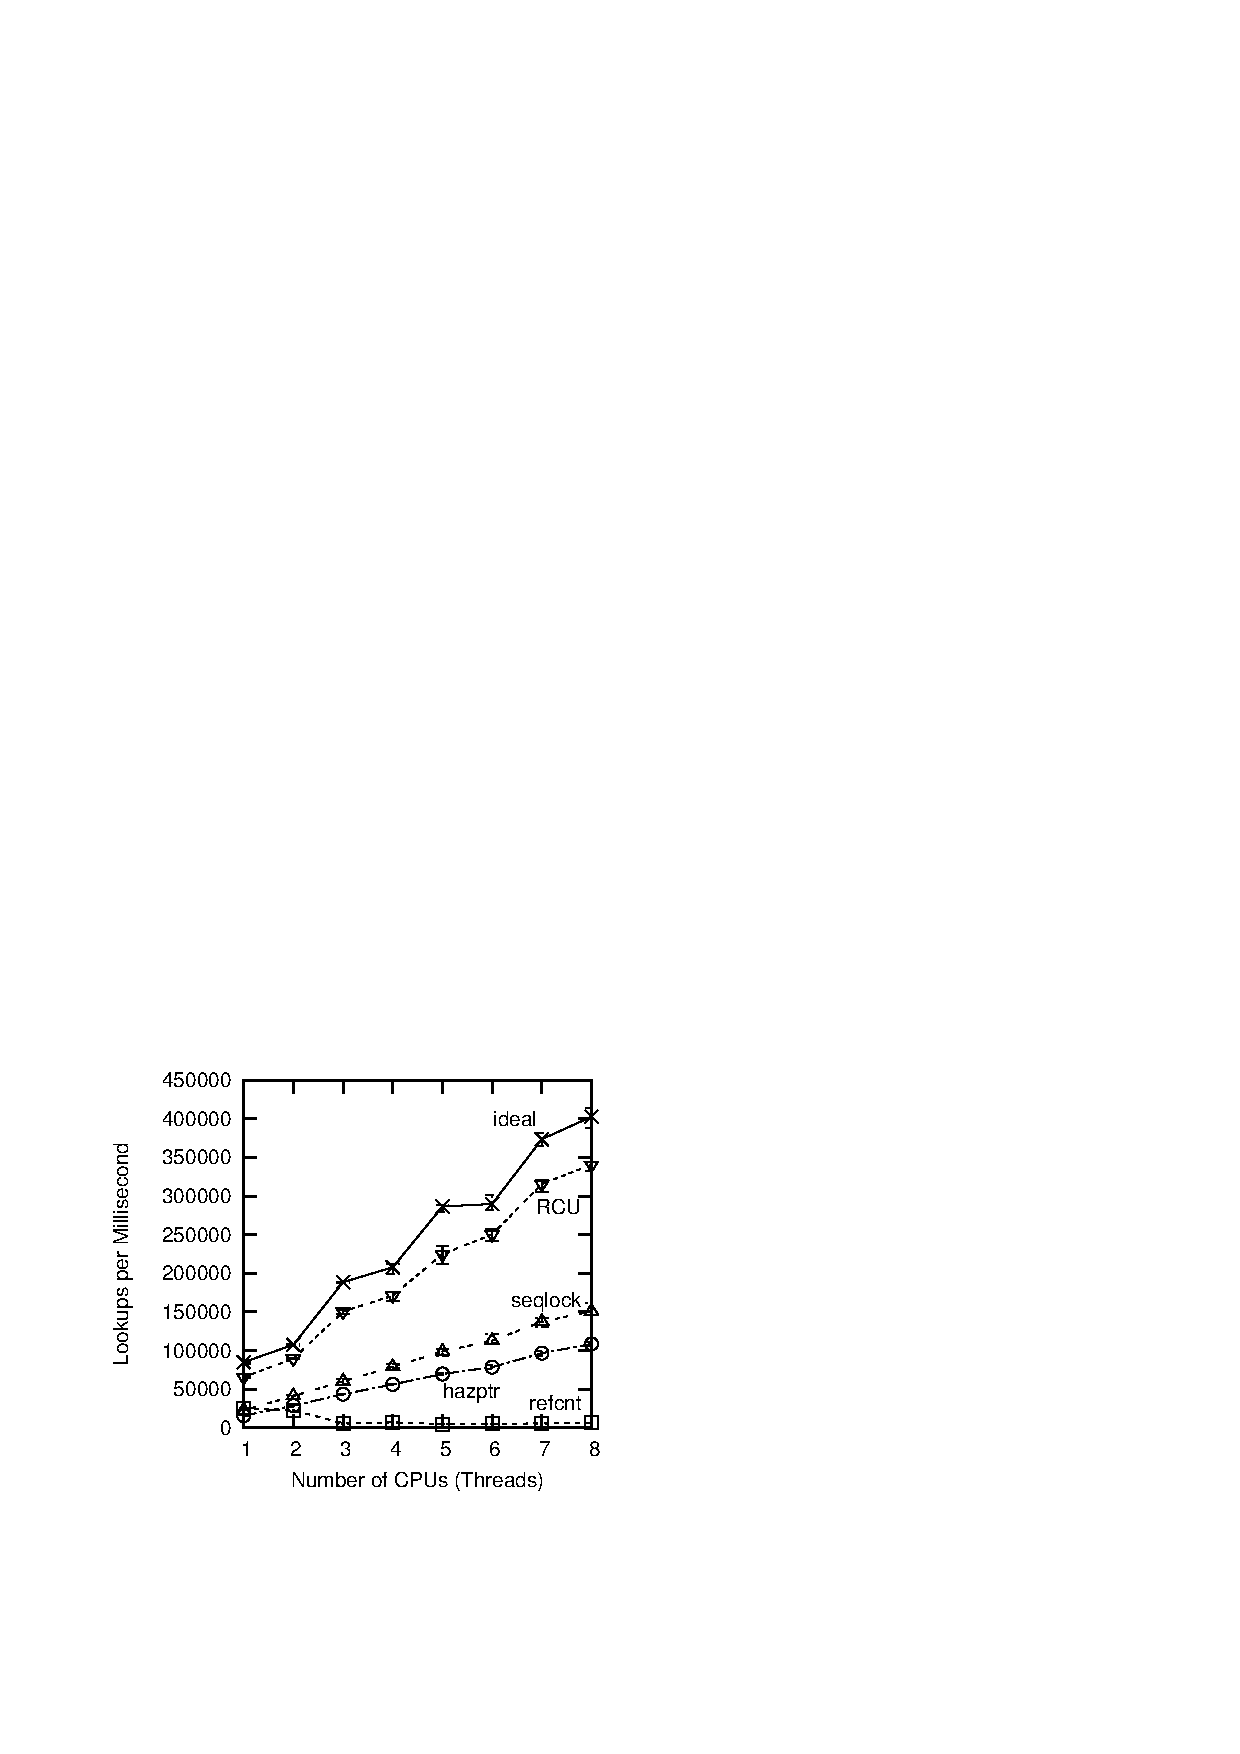
\includegraphics{CodeSamples/defer/perf-rcu}}
\caption{Pre-BSD Routing Table Protected by RCU}
\label{fig:defer:Pre-BSD Routing Table Protected by RCU}
\end{figure}

Figure~\ref{fig:defer:Pre-BSD Routing Table Protected by RCU}
는 읽기 전용 워크로드에서의 성능을 보입니다.
RCU 는 상당히 잘 확장되며 거의 이상적인 성능을 제공합니다.
하지만, 이 데이터는 \co{rcu_read_lock()} 과 \co{rcu_read_unlock()} 에 작은 양의
코드를 생성하는 userspace
RCU~\cite{MathieuDesnoyers2009URCU,PaulMcKenney2013LWNURCU} 의 \co{RCU_SIGNAL}
버전을 사용해 만들어졌습니다.
\co{rcu_read_lock()} 과 \co{rcu_read_unlock()} 에 어떤 코드도 생성하지 않는
QSBR 버전의 RCU 를 사용하면 어떻게 될까요?
(RCU QSBR 에 대한 논의를 위해선
Section~\ref{sec:defer:Introduction to RCU},
그리고 특히
Figure~\ref{fig:defer:QSBR: Waiting for Pre-Existing Readers} 를 보시기
바랍니다.)

이에 대한 답이 RCU QSBR 의 성능과 확장성은 실제로 이상적인 동기화 없는
워크로드의 것을 넘어섬을 보이는
Figure~\ref{fig:defer:Pre-BSD Routing Table Protected by RCU QSBR}
에 보여져 있습니다.

\iffalse

Figure~\ref{fig:defer:Pre-BSD Routing Table Protected by RCU}
shows the performance on the read-only workload.
RCU scales quite well, and offers nearly ideal performance.
However, this data was generated using the \co{RCU_SIGNAL}
flavor of userspace
RCU~\cite{MathieuDesnoyers2009URCU,PaulMcKenney2013LWNURCU},
for which \co{rcu_read_lock()} and \co{rcu_read_unlock()}
generate a small amount of code.
What happens for the QSBR flavor of RCU, which generates no code at all
for \co{rcu_read_lock()} and \co{rcu_read_unlock()}?
(See Section~\ref{sec:defer:Introduction to RCU},
and especially
Figure~\ref{fig:defer:QSBR: Waiting for Pre-Existing Readers},
for a discussion of RCU QSBR\@.)

The answer to this is shown in
Figure~\ref{fig:defer:Pre-BSD Routing Table Protected by RCU QSBR},
which shows that RCU QSBR's performance and scalability actually exceeds
that of the ideal synchronization-free workload.

\fi

\QuickQuizSeries{%
\QuickQuizB{
	잠깐요, 뭐라고요???
	어떻게 RCU QSBR 이 이상적인 것보다 나을 수 있죠?
	어떤 쓰레기 같은 이상에 대한 정의가 그것이 모든 가능한 결과 중 최선이
	아니게 할 수 있죠???

	\iffalse

	Wait, what???
	How can RCU QSBR possibly be better than ideal?
	Just what rubbish definition of ideal would fail to be the best
	of all possible results???

	\fi

}\QuickQuizAnswerB{
	훌륭한 질문이고, 이에 대한 답은 현대의 CPU 와 컴파일러는 굉장히
	복잡하다는 것입니다.
	하지만 거기까지 가기 전에, RCU QSBR 의 성능 이득은 코어당 하나의
	하드웨어 쓰레드가 제공되는 세계에서만 나타남을 알아둘 가치가 있습니다.
	시스템에 부하가 완전히 걸리고 나면, RCU QSBR 의 성능은 이상적인 것의
	수준으로 떨어집니다.

	RCU 버전의 \co{route_lookup()} 탐색 반복문은 실제 순차적 버전의 것보다
	x86 명령을 하나더 가지는데, 이는 \co{cmp}, \co{je}, \co{mov}, \co{cmp},
	\co{lea}, and \co{jne} 순서에서의 \co{lea} 입니다.
	이 추가된 명령은 RCU 버전의 \co{route_entry} 구조체의 시작지점에 있는
	\co{rcu_head} 구조체 때문으로, 이 때문에 순차적 버전과 달리 RCU 버전의
	\co{->re_next.next} 포인터는 0이 아닌 오프셋을 갖습니다.
	1980년대로 돌아가 보면, 이 추가적인 \co{lea} 명령은 RCU 버전이 느려지는
	결과를 낼 수도 있었습니다만, 우린 지금 21세기에 있으며, 1980년대는 한참
	지났습니다.

	\iffalse

	This is an excellent question, and the answer is that modern
	CPUs and compilers are extremely complex.
	But before getting into that, it is well worth noting that
	RCU QSBR's performance advantage appears only in the
	one-hardware-thread-per-core regime.
	Once the system is fully loaded, RCU QSBR's performance drops
	back to ideal.

	The RCU variant of the \co{route_lookup()} search loop actually
	has one more x86 instruction than does the sequential version,
	namely the \co{lea} in the sequence
	\co{cmp}, \co{je}, \co{mov}, \co{cmp}, \co{lea}, and \co{jne}.
	This extra instruction is due to the \co{rcu_head} structure
	at the beginning of the RCU variant's \co{route_entry} structure,
	so that, unlike the sequential variant, the RCU variant's
	\co{->re_next.next} pointer has a non-zero offset.
	Back in the 1980s, this additional \co{lea} instruction might
	have reliably resulted in the RCU variant being slower, but we
	are now in the 21\textsuperscript{st} century, and the 1980s
	are long gone.

	\fi

	하지만
	\cref{sec:cpu:Pipelined CPUs}
	를 주의 깊게 읽은 여러분들은 이미 이 모든 걸 알고 있을 겁니다!

	이런 반직관적인 결과는 물론 현대 마이크로프로세서에서의 모든 성능
	결과는 약간 회의적으로 보아져야 함을 의미합니다.
	이론상, 이상적인 것보다 나은 성능을 얻는다는 것은 정말 말이 안됩니다만,
	현대의 마이크로프로세서에서는 정말로 일어날 수 있는 일입니다.
	그런 결과는 축복받은 초선형적 성능향상 (그런 예 중 하나를 위해
	Section~\ref{sec:SMPdesign:Beyond Partitioning} 을 보세요) 비슷한 걸로
	생각 될 수 있는데, 즉, 흥미롭지만 또한 실용적 중요도는 제한된다는
	것입니다.
	그러나, RCU 의 강점 중 하나는 그 읽기 쪽 오버헤드가 무척 낮아서 이와
	같은 작은 효과가 실제 성능 측정에도 보여질 수 있다는 것입니다.

	\iffalse

	But those of you who read
	\cref{sec:cpu:Pipelined CPUs}
	carefully already knew all of this!

	These counter-intuitive results of course means that any
	performance result on modern microprocessors must be subject to
	some skepticism.
	In theory, it really does not make sense to obtain performance
	results that are better than ideal, but it really can happen
	on modern microprocessors.
	Such results can be thought of as similar to the celebrated
	super-linear speedups (see
	Section~\ref{sec:SMPdesign:Beyond Partitioning}
	for one such example), that is, of interest but also of limited
	practical importance.
	Nevertheless, one of the strengths of RCU is that its read-side
	overhead is so low that tiny effects such as this one are visible
	in real performance measurements.

	\fi

\begin{figure}[tb]
\centering
\resizebox{2.5in}{!}{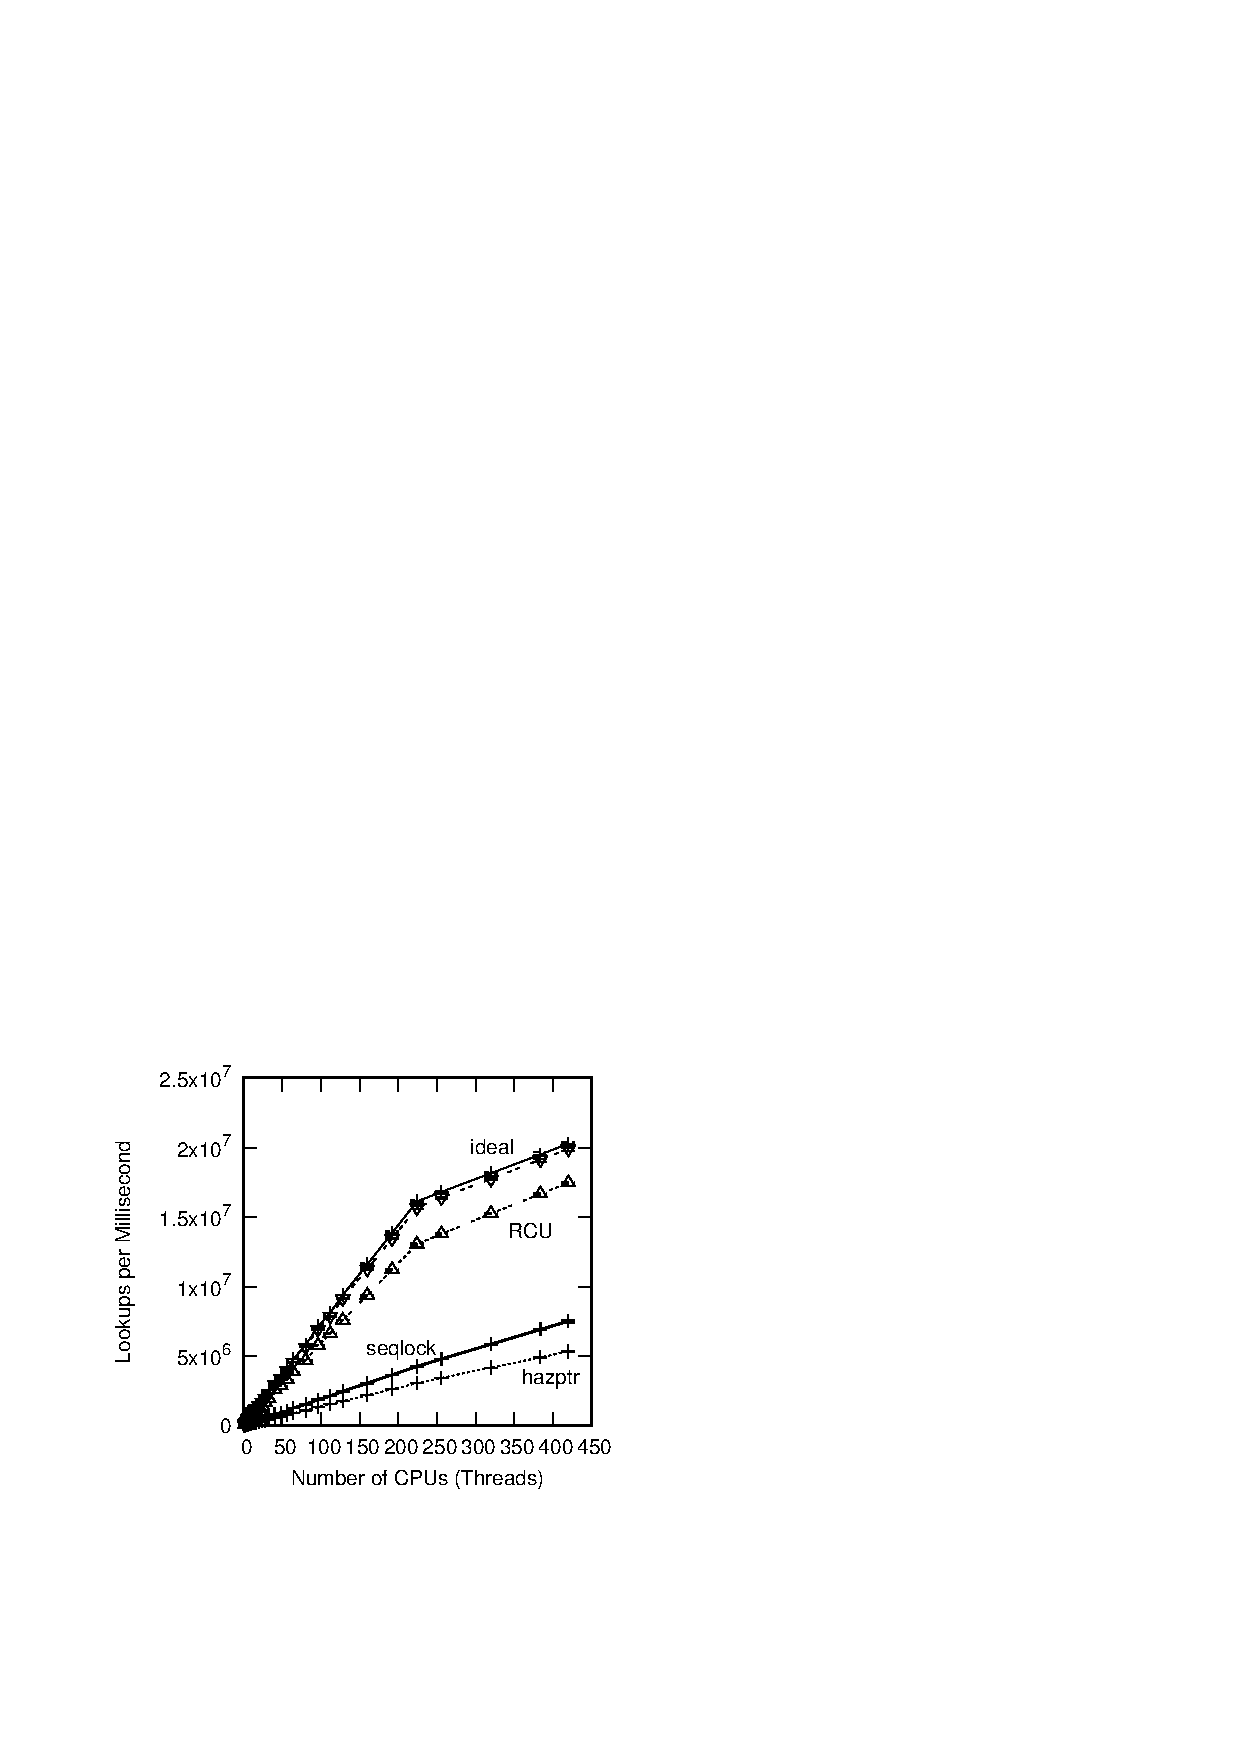
\includegraphics{CodeSamples/defer/perf-rcu-qsbr-qq}}
\caption{Pre-BSD Routing Table Protected by RCU QSBR With Non-Initial \tco{rcu_head}}
\label{fig:defer:Pre-BSD Routing Table Protected by RCU QSBR With Non-Initial rcu-head}
\end{figure}

	이는 \co{rcu_head} 구조체가 \co{->re_next.next} 포인터가 0 오프셋을
	갖게끔 옮겨져서 순차적 버전과 동일하게 되면 어떻게 되는지 질문을 하게
	만듭니다.
	그에 대한 답은
	Figure~\ref{fig:defer:Pre-BSD Routing Table Protected by RCU QSBR With Non-Initial rcu-head}
	에 보여져 있듯, RCU QSBR 의 성능이 여전히 이상적인 것에 근접하지만
	이상적인 것을 넘어서지는 않게 한다는 것입니다.

	\iffalse

	This raises the question as to what would happen if the
	\co{rcu_head} structure were to be moved so that RCU's
	\co{->re_next.next} pointer also had zero offset, just the
	same as the sequential variant.
	And the answer, as can be seen in
	Figure~\ref{fig:defer:Pre-BSD Routing Table Protected by RCU QSBR With Non-Initial rcu-head},
	is that this causes RCU QSBR's performance to decrease to where
	it is still very nearly ideal, but no longer super-ideal.

	\fi

}\QuickQuizEndB
%
\QuickQuizE{
	RCU QSBR 의 읽기 성능이 그렇게 좋은데, 왜 다른 userspace 버전을
	신경쓰죠?

	\iffalse

	Given RCU QSBR's read-side performance, why bother with any
	other flavor of userspace RCU?

	\fi

}\QuickQuizAnswerE{
	RCU QSBR 은 허용될 수 없을 수도 있는 어플리케이션 전체의 제약을
	요구하기 때문인데, 예를 들면 어플리케이션 내의 모든 각각의 쓰레드가
	정기적으로 quiescent state 를 지나야 한다는 것입니다.
	다른 것들 중에서도, 이는 RCU QSBR 이 다른 종류의 userspace
	RCU~\cite{PaulMcKenney2013LWNURCU} 에 의해 더 잘 도움받을 수도 있는
	라이브러리 작성자에게는 도움이 될 수 있다는 것을 의미합니다.

	\iffalse

	Because RCU QSBR places constraints on the overall application
	that might not be tolerable,
	for example, requiring that each and every thread in the
	application regularly pass through a quiescent state.
	Among other things, this means that RCU QSBR is not helpful
	to library writers, who might be better served by other
	flavors of userspace RCU~\cite{PaulMcKenney2013LWNURCU}.

	\fi

}\QuickQuizEndE
}

\begin{figure}[tb]
\centering
\resizebox{2.5in}{!}{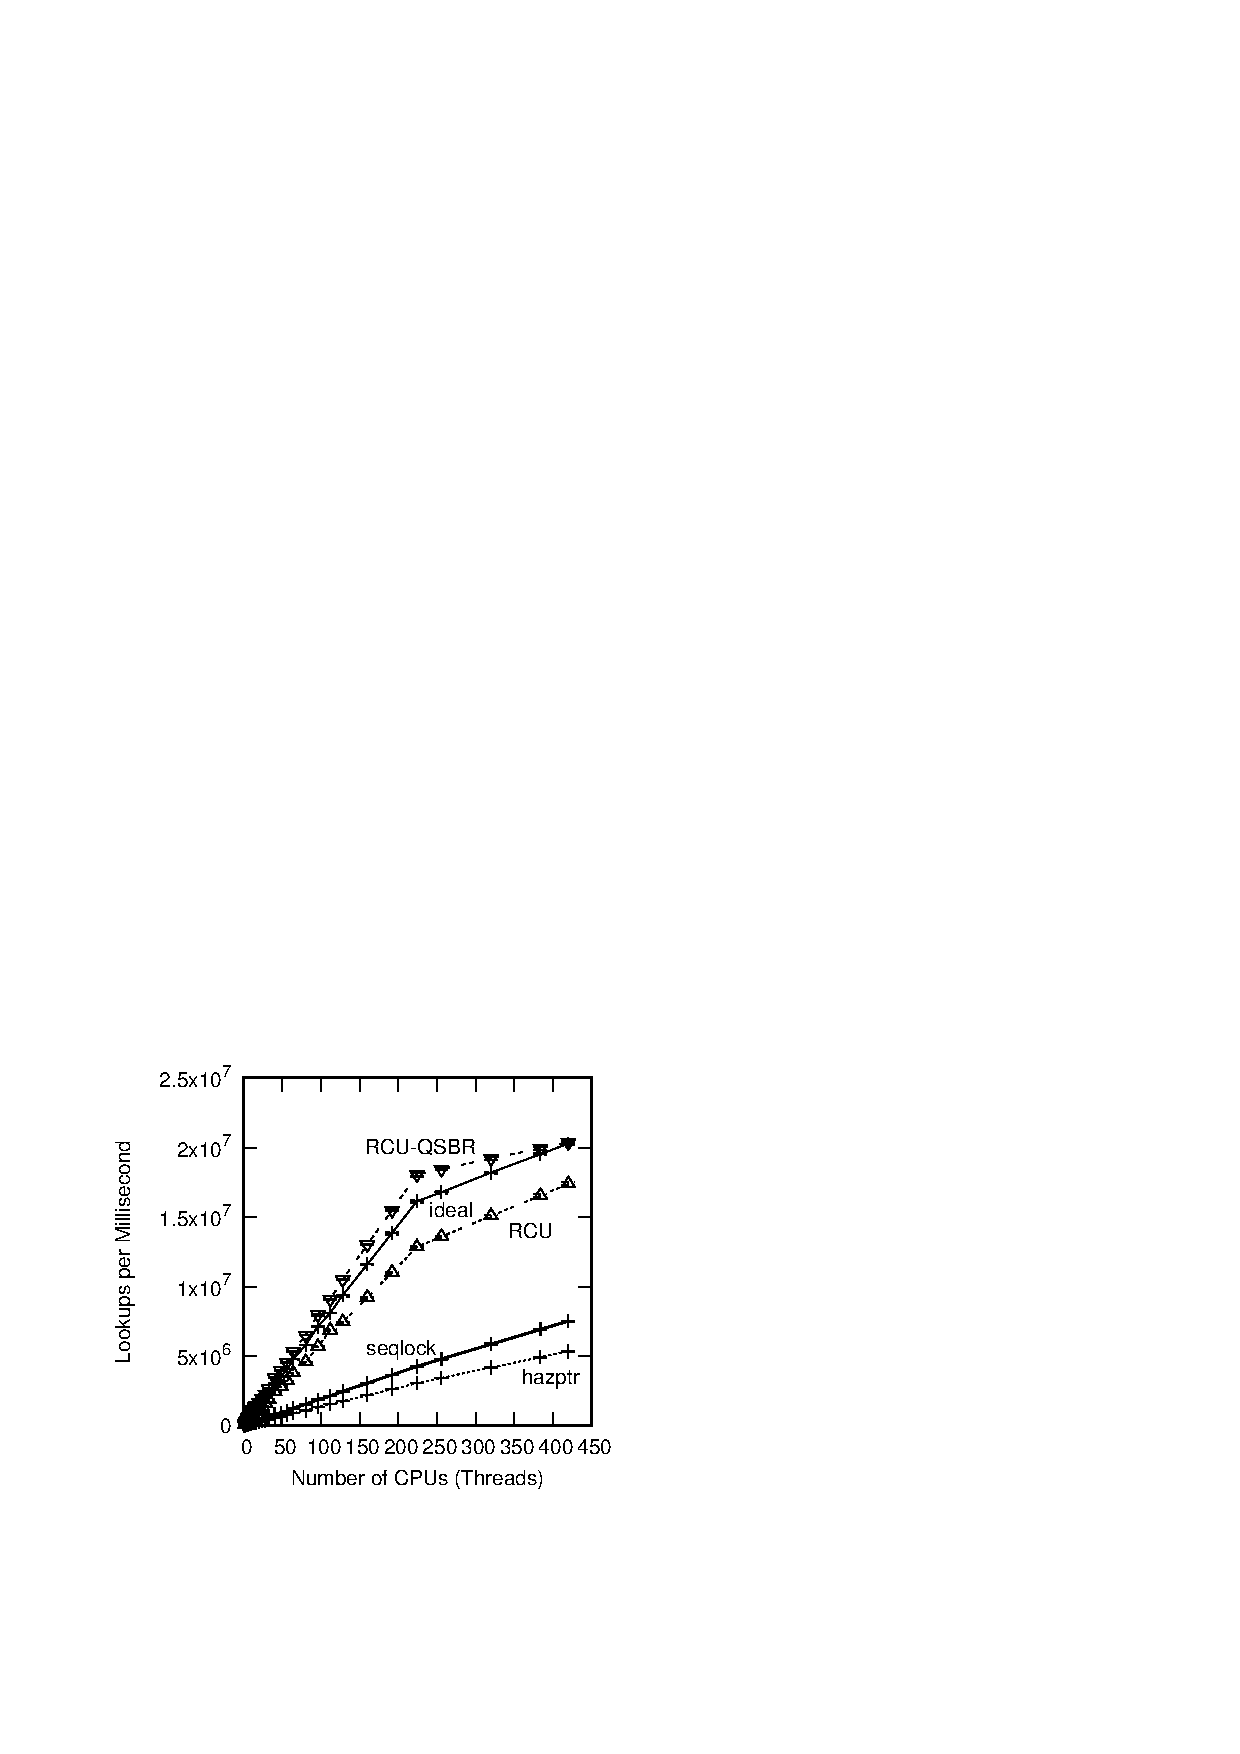
\includegraphics{CodeSamples/defer/perf-rcu-qsbr}}
\caption{Pre-BSD Routing Table Protected by RCU QSBR}
\label{fig:defer:Pre-BSD Routing Table Protected by RCU QSBR}
\end{figure}

\subsubsection{RCU is a Reader-Writer Lock Replacement}
\label{sec:defer:RCU is a Reader-Writer Lock Replacement}

리눅스 커널에서의 RCU 의 가장 흔한 사용처는 아마도 읽기가 집중적인 상황에서의
reader-writer 락킹 대체일 겁니다.
그러나, 이런 RCU 사용은 처음에 제게 즉각적으로 적절하게 느껴지지 않았고, 실제로
저는 1990년대 초에 범용 RCU 구현을 만들기 전에 가벼운 reader-writer 락을
구현하기로 했습니다~\cite{WilsonCHsieh92a}.\footnote{
	2.4 리눅스 커널의 \co{brlock} 과, 더 최신의 리눅스 커널의 \co{lglock}
	과 비슷합니다.}
이 가벼운 reader-writer 락으로 제가 하고자 했던 모든 것은 결국 RCU 를 이용해
구현되었습니다.
사실, 그건 이 가벼운 reader-writer 락이 처음 사용되기 3년이나 전의
일이었습니다.
정말 바보가 된 것 같았죠!

RCU 와 reader-writer 락킹 사이의 핵심 유사성은 둘 다 병렬로 구생될 수 있는
read-side 크리티컬 섹션을 갖는다는 것입니다.
실제로, 어떤 경우에는 RCU API 멤버들을 연관된 reader-writer 락 API 멤버들로
대체하는게 가능합니다.
하지만 무엇보다, 왜 그런걸 신경쓰죠?

\iffalse

Perhaps the most common use of RCU within the Linux kernel is as
a replacement for reader-writer locking in read-intensive situations.
Nevertheless, this use of RCU was not immediately apparent to me
at the outset, in fact, I chose to implement a lightweight reader-writer
lock~\cite{WilsonCHsieh92a}\footnote{
	Similar to \co{brlock} in the 2.4 Linux kernel and to
	\co{lglock} in more recent Linux kernels.}
before implementing a general-purpose RCU implementation
back in the early 1990s.
Each and every one of the uses I envisioned for the lightweight reader-writer
lock was instead implemented using RCU\@.
In fact, it was more than
three years before the lightweight reader-writer lock saw its first use.
Boy, did I feel foolish!

The key similarity between RCU and reader-writer locking is that
both have read-side critical sections that can execute in parallel.
In fact, in some cases, it is possible to mechanically substitute RCU API
members for the corresponding reader-writer lock API members.
But first, why bother?

\fi

RCU 의 장점은 성능, 데드락 내성, 그리고 리얼타임 응답시간을 포함합니다.
물론, RCU 의 제한점들도 존재하는데 읽기 쓰레드와 업데이트 쓰레드가 동시에
수행된다는 사실, 낮은 우선순위 RCU 읽기 쓰레드가 높은 우선순위 쓰레드를 grace
period 하나가 지나갈 때까지 블록시킨다는 것, 그리고 grace period 응답시간이 수
밀리세컨드까지 길어질 수 있다는 점이 포함됩니다.
이런 장점과 한계점들이 다음 문단들에서 논의됩니다.

\iffalse

Advantages of RCU include performance,
deadlock immunity, and realtime latency.
There are, of course, limitations to RCU, including the fact that
readers and updaters run concurrently, that low-priority RCU readers
can block high-priority threads waiting for a grace period to elapse,
and that grace-period latencies can extend for many milliseconds.
These advantages and limitations are discussed in the following paragraphs.

\fi

\paragraph{Performance}

\begin{figure}[tb]
\centering
\resizebox{2.5in}{!}{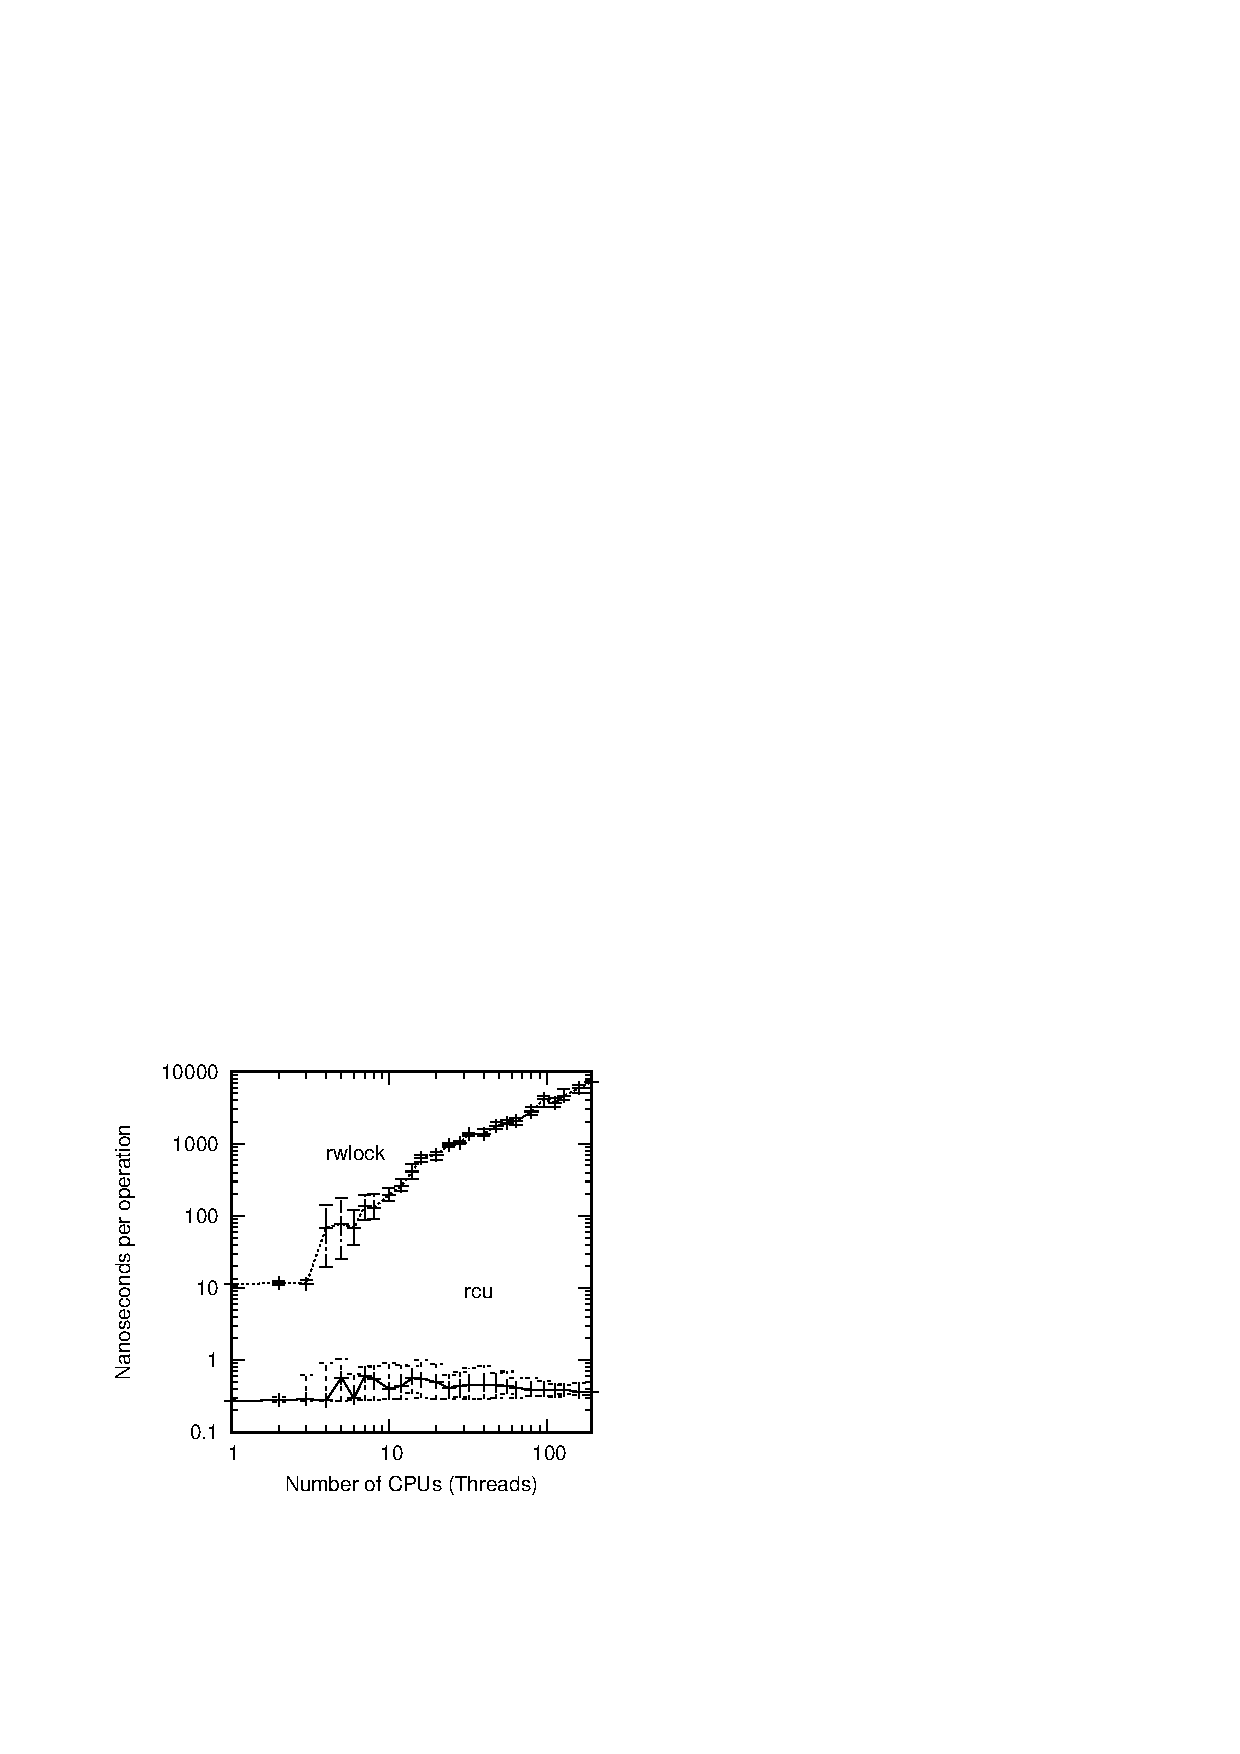
\includegraphics{defer/rwlockRCUperf}}
\caption{Performance Advantage of RCU Over Reader-Writer Locking}
\label{fig:defer:Performance Advantage of RCU Over Reader-Writer Locking}
\end{figure}

리눅스 커널 RCU 의 reader-writer 락킹 대비 읽기 성능 장점이
448 개 2.10\,GHz Intel x86 CPU 시스템에서 측정되어 만들어진
Figure~\ref{fig:defer:Performance Advantage of RCU Over Reader-Writer Locking}
에 보여져 있습니다.

\iffalse

The read-side performance advantages of Linux-kernel RCU over
reader-writer locking are shown in
Figure~\ref{fig:defer:Performance Advantage of RCU Over Reader-Writer Locking},
which was generated on a 448-CPU 2.10\,GHz Intel x86 system.

\fi

\QuickQuizSeries{%
\QuickQuizB{
	뭐요?
	2.10\,GHz 에서의 클락 시간은 약 500\,picosecond 인데 RCU 가
	300-picosecond 도 안되는 오버헤드를 갖는다는 말을 나더러 믿으라구요?

	\iffalse

	WTF?
	How the heck do you expect me to believe that RCU can have less
	than a 300-picosecond overhead when the clock period at 2.10\,GHz
	is almost 500\,picoseconds?

	\fi

}\QuickQuizAnswerB{
	우선, 이 측정을 위해 사용된 반복문이 다음과 같음을 고려합시다:

	\iffalse

	First, consider that the inner loop used to
	take this measurement is as follows:

	\fi

\begin{VerbatimN}
	for (i = nloops; i >= 0; i--) {
		rcu_read_lock();
		rcu_read_unlock();
	}
\end{VerbatimN}

	다음으로, 실질적인 \co{rcu_read_lock()} 과 \co{rcu_read_unlock()} 의
	정의를 생각해 봅시다:

	\iffalse

	Next, consider the effective definitions of \co{rcu_read_lock()}
	and \co{rcu_read_unlock()}:

	\fi

\begin{VerbatimN}
#define rcu_read_lock()   barrier()
#define rcu_read_unlock() barrier()
\end{VerbatimN}

	이 정의들은 메모리 참조에 연관되는 컴파일러의 코드 이동 최적화를
	제약하지만, 그것들 자체 내에는 어떤 명령도 넣지 않습니다.
	하지만, 이 반복문 변수가 레지스터에 관리된다면, \co{i} 로의 액세스는
	메모리 참조로 취급되지 않습니다.
	더욱이, 컴파일러는 loop unrolling 을 알 수 있어, 결과적인 코드가 단순히
	\co{i} 값을 1보다 큰 어떤 값으로 증가시키는 것으로 여러 횟수의 반복문
	수행을 ``해내는'' 코드를 만들 수 있습니다.

	따라서 267 picoseconds 의 ``측정'' 은 시간 측정을 \co{rcu_read_lock()}
	과 \co{rcu_read_unlock()} 호출을 포함하는 이 내부 반복문을 통과하는
	반복 횟수로 나눈 것에 이 loop-unrolling 으로 \co{i} 조정 코드를 나눈
	것을 더한 고정된 오버헤드입니다.
	그리고 그래서, 이 측정은 실제로 에러를 포함하고 있으며, 실제로
	오버헤드를 수십 수백배로 부풀려서 이야기 하고 있습니다.
	어쨌건, 만들어진 기계 명령어의 관점에서, \co{rcu_read_lock()} 과
	\co{rcu_read_unlock()} 의 오버헤드는 정확히 제로입니다.

	267 picosecond 의 측정된 시간이 과장된 수치임이 드러나는 건 매일 있는
	일은 분명 아닙니다!

	\iffalse

	These definitions constrain compiler code-movement optimizations
	involving memory references, but emit no instructions in and
	of themselves.
	However, if the loop variable is maintained in a register,
	the accesses to \co{i} will not count as memory references.
	Furthermore, the compiler can do loop unrolling,
	allowing the resulting code to ``execute'' multiple passes
	through the loop body simply by incrementing \co{i} by
	some value larger than the value 1.

	So the ``measurement'' of 267 picoseconds is simply the fixed
	overhead of the timing measurements divided by the number of
	passes through the inner loop containing the calls
	to \co{rcu_read_lock()} and \co{rcu_read_unlock()}, plus
	the code to manipulate \co{i} divided by the loop-unrolling
	factor.
	And therefore, this measurement really is in error, in fact,
	it exaggerates the overhead by an arbitrary number of orders
	of magnitude.
	After all, in terms of machine instructions emitted, the actual
	overheads of \co{rcu_read_lock()} and of \co{rcu_read_unlock()}
	are each precisely zero.

	It certainly is not just every day that a timing measurement
	of 267 picoseconds turns out to be an overestimate!

	\fi
}\QuickQuizEndB

\QuickQuizM{
	이 책의 초기 버전에서는 RCU 읽기 오버헤드가 1 picosecond 미만이라 하지
	않았나요?
	무슨 일이 있었던 거죠???

	\iffalse

	Didn't an earlier release of this book show RCU read-side
	overhead way down in the sub-picosecond range?
	What happened???

	\fi

}\QuickQuizAnswerM{
	훌륭한 기억력이군요!!!
	어떤 초기 버전에서의 오버헤드는 실제로 약 100 femtosecond 이었습니다.

	그사이 무슨 일이 있었느냐면, RCU 사용처가 리눅스 커널 내에 더욱 널리
	퍼졌는데, page fault 처리 코드도 여기 포함됩니다.
	그때로 돌아가면, \co{rcu_read_lock()} 과 \co{rcu_read_unlock()} 은
	\co{CONFIG_PREEMPT=n} 커널에서 완전히 아무 일도 하지 않았습니다.
	불행히도, 그 상황은 컴파일러가 page fault 되는 메모리 액세스를 RCU
	read-side 크리티컬 섹션 내로 재배치 할 수 있게 했습니다.
	물론, page fault 는 블록될 수 있으며, 따라서 이 크리티컬 섹션을
	망가지게 합니다.

	\iffalse

	Excellent memory!!!
	The overhead in some early releases was in fact roughly
	100~femtoseconds.

	What happened was that RCU usage spread more broadly through the
	Linux kernel, including into code that takes page faults.
	Back at that time, \co{rcu_read_lock()} and \co{rcu_read_unlock()}
	were complete no-ops in \co{CONFIG_PREEMPT=n} kernels.
	Unfortunately, that situation allowed the compiler to reorder
	page-faulting memory accesses into RCU read-side critical
	sections.
	Of course, page faults can block, which destroys those critical
	section.

	\fi

	이건 이론적 문제만이 아니었습니다:
	그로 인한 문제가 실제로 2019년에 이야기 되었습니다.
	\ppl{Herber}{Xu} 는 이 문제를 분석했고 \ppl{Linus}{Torvalds} 는
	\co{rcu_read_lock()} 과 \co{rcu_read_unlock()} 이 무조건적으로
	\co{barrier()} 호출을 포함하게 하는 커밋을 대기열에
	올렸습니다~\cite{LinusTorvalds2019:RCUreader.barrier}.
	그리고 \co{barrier()} 가 코드를 추가하진 않지만, 컴파일러 최적화를
	제한합니다.
	따라서 널리 퍼져있는 RCU 사용처의 비용은 \co{rcu_read_lock()} 과
	\co{rcu_read_unlock()} 오버헤드보다 약간 더 높아집니다.

	물론, 더 오래전의 결과는
	Figure~\ref{fig:defer:Performance Advantage of RCU Over Reader-Writer Locking}
	에서 보인 것과 다른 시스템에서 얻어진 겁니다.
	그래서 뭐가 더 영향을 끼쳤을까요, Linus 의 커밋 또는 시스템 변경?
	이 질문은 독자 여러분의 연습문제로 남겨둡니다.

	\iffalse

	Nor was this a theoretical problem:
	A failure actually manifested in 2019.
	\ppl{Herbert}{Xu} tracked down this failure down and
	\ppl{Linus}{Torvalds}
	therefore queued a commit to upgrade \co{rcu_read_lock()} and
	\co{rcu_read_unlock()} to unconditionally include a call to
	\co{barrier()}~\cite{LinusTorvalds2019:RCUreader.barrier}.
	And although \co{barrier()} emits no code, it does constrain
	compiler optimizations.
	And so the price of widespread RCU usage is slightly higher
	\co{rcu_read_lock()} and \co{rcu_read_unlock()} overhead.

	Of course, it is also the case that the older results were obtained
	on a different system than were those shown in
	Figure~\ref{fig:defer:Performance Advantage of RCU Over Reader-Writer Locking}.
	So which change had the most effect, Linus's commit or the change in
	the system?
	This question is left as an exercise to the reader.

	\fi

}\QuickQuizEndM

\QuickQuizE{
	Figure~\ref{fig:defer:Performance Advantage of RCU Over Reader-Writer Locking}
	의 \co{rcu} 에는 왜그리 큰 편차가 존재하는 거죠?

	\iffalse

	Why is there such large variation for the \co{rcu} trace in
	Figure~\ref{fig:defer:Performance Advantage of RCU Over Reader-Writer Locking}?

	\fi

}\QuickQuizAnswerE{
	이는 log-log 그림이며, 따라서 크게 보이는 \co{rcu} 편차는 실제로는 수백
	picosecond 에 불과함을 명심하세요.
	그리고 그건 무엇이든 그것을 일으킬 수 있는 무척 짧은 시간입니다.
	하지만, 편차가 CPU 수가 작든 크든 감소된다는 걸로 보아, 한가지 가능한
	가설은 이 편차는 하나의 CPU 에서 다른 CPU 로의 migration 때문이라는
	것입니다.

	그래요, 이 측정은 인터럽트가 불능화 된 채로 취해졌습니다만, 게스트 OS
	내에서 취해졌으므로, 하이퍼바이저 단계에서의 preemption 은 가능합니다.
	이 게스트 OS 들을 리얼타임 우선순위로 수행함으로써 이런 편차를 줄이려는
	노력은 (Joel Fernandes 에 의해 제안되었습니다) 독자 여러분의 연습문제로
	남겨두겠습니다.

	\iffalse

	Keep in mind that this is a log-log plot, so those large-seeming
	\co{rcu} variances in reality span only a few hundred picoseconds.
	And that is such a short time that anything could cause it.
	However, given that the variance decreases with both small and
	large numbers of CPUs, one hypothesis is that the variation is
	due to migrations from one CPU to another.

	Yes, these measurements were taken with interrupts disabled, but
	they were also taken within a guest OS, so that preemption was
	still possible at the hypervisor level.
	Attempting to reduce these variations by running the guest OSes
	at real-time priority (as suggested by Joel Fernandes) is left
	as an exercise for the reader.

	\fi

}\QuickQuizEndE
}                 % End of \QuickQuizSeries

Reader-writer 락킹은 단일 CPU 에서 RCU 보다 수십배 느리며, 192~CPU 에서는
\emph{수만} 배보다 더 느리다는 것을 보시기 바랍니다.
대조적으로, RCU 는 상당히 잘 확장합니다.
두 경우 모드, 에러 바들은 30회의 측정 결과 전체 범위를 보이며, 선은 그 중간값을
보입니다.

\iffalse

Note that reader-writer locking is more than an order of magnitude slower
than RCU on a single CPU, and is more than \emph{four} orders of magnitude
slower on 192~CPUs.
In contrast, RCU scales quite well.
In both cases, the error bars cover the full range of the measurements
from 30~runs, with the line being the median.

\fi

\begin{figure}[tb]
\centering
\resizebox{2.5in}{!}{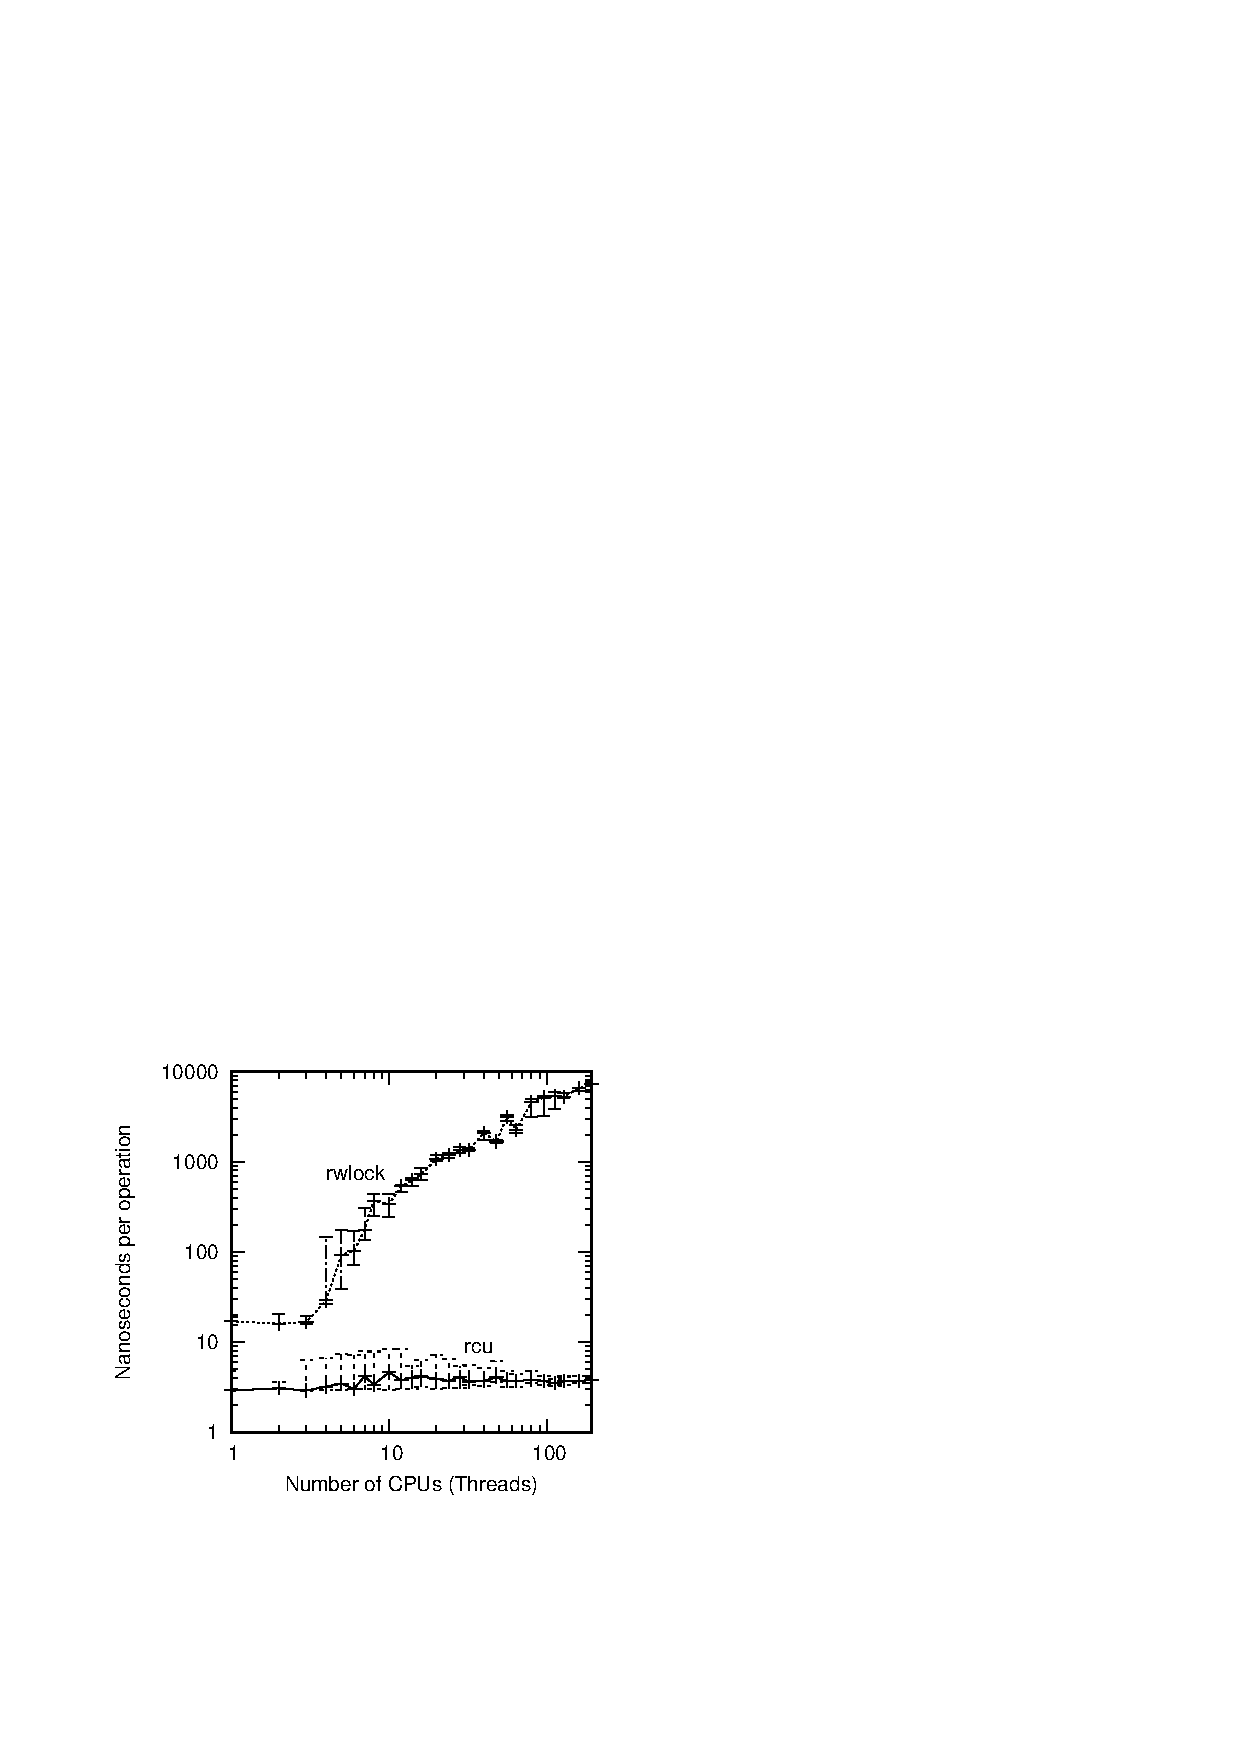
\includegraphics{defer/rwlockRCUperfPREEMPT}}
\caption{Performance Advantage of Preemptible RCU Over Reader-Writer Locking}
\label{fig:defer:Performance Advantage of Preemptible RCU Over Reader-Writer Locking}
\end{figure}

더 정확한 그림은 \co{CONFIG_PREEMPT} 커널에서 얻어질 수 있겠지만, 448rodml
2.10\,GHz x86 CPU 시스템에서 측정된
Figure~\ref{fig:defer:Performance Advantage of Preemptible RCU Over Reader-Writer Locking}
에 보이듯 RCU 는 여전히 단일 CPU 에서 약 일곱배, 192~CPU 에서 수천배
reader-writer 락보다 빠릅니다.
큰 수의 CPU 에서 reader-writer 락킹의 높은 편차값을 보세요.
에러바는 데이터의 전체 범위를 그립니다.

\iffalse

A more moderate view may be obtained from a \co{CONFIG_PREEMPT} kernel,
though RCU still beats reader-writer locking by between a factor of seven
on a single CPU and by three orders of magnitude on 192~CPUs, as shown in
Figure~\ref{fig:defer:Performance Advantage of Preemptible RCU Over Reader-Writer Locking},
which was generated on the same 448-CPU 2.10\,GHz x86 system.
Note the high variability of reader-writer locking at larger numbers of CPUs.
The error bars span the full range of data.

\fi

\QuickQuiz{
	시스템은 448 개의 하드웨어 쓰레드를 갖는데, 왜 192~CPU 까지만
	측정하나요?

	\iffalse

	Given that the system had no fewer than 448~hardware threads,
	why only 192~CPUs?

	\fi

}\QuickQuizAnswer{
	이 데이터를 생성하는데 사용된 스크립트 (\path{rcusclae.sh}) 는 모아지는
	지점들의 각 집합을 위해 게스트 운영체제를 시작하며, 이 특정
	시스템에서는 \co{qemu} 와 KVM 이 모두 특정 게스트 OS 에 설정될 수 있는
	CPU 갯수에 제한을 두기 때문입니다.
	그래요, 조금 더 많은 CPU 를 사용하는 것도 가능하겠습니다만 256 은
	불가능하다는 점을 생각할 때 이진수 관점에서 192 는 괜찮은 어림수입니다.

	\iffalse

	Because the script (\path{rcuscale.sh}) that generates this data
	spawn a guest operating system for each set of points gathered,
	and on this particular system, both \co{qemu} and KVM limit the
	number of CPUs that may be configured into a given guest OS\@.
	Yes, it would have been possible to run a few more CPUs, but
	192 is a nice round number from a binary perspective, given
	that 256 is infeasible.

	\fi
}\QuickQuizEnd

\begin{figure}[tb]
\centering
\resizebox{2.5in}{!}{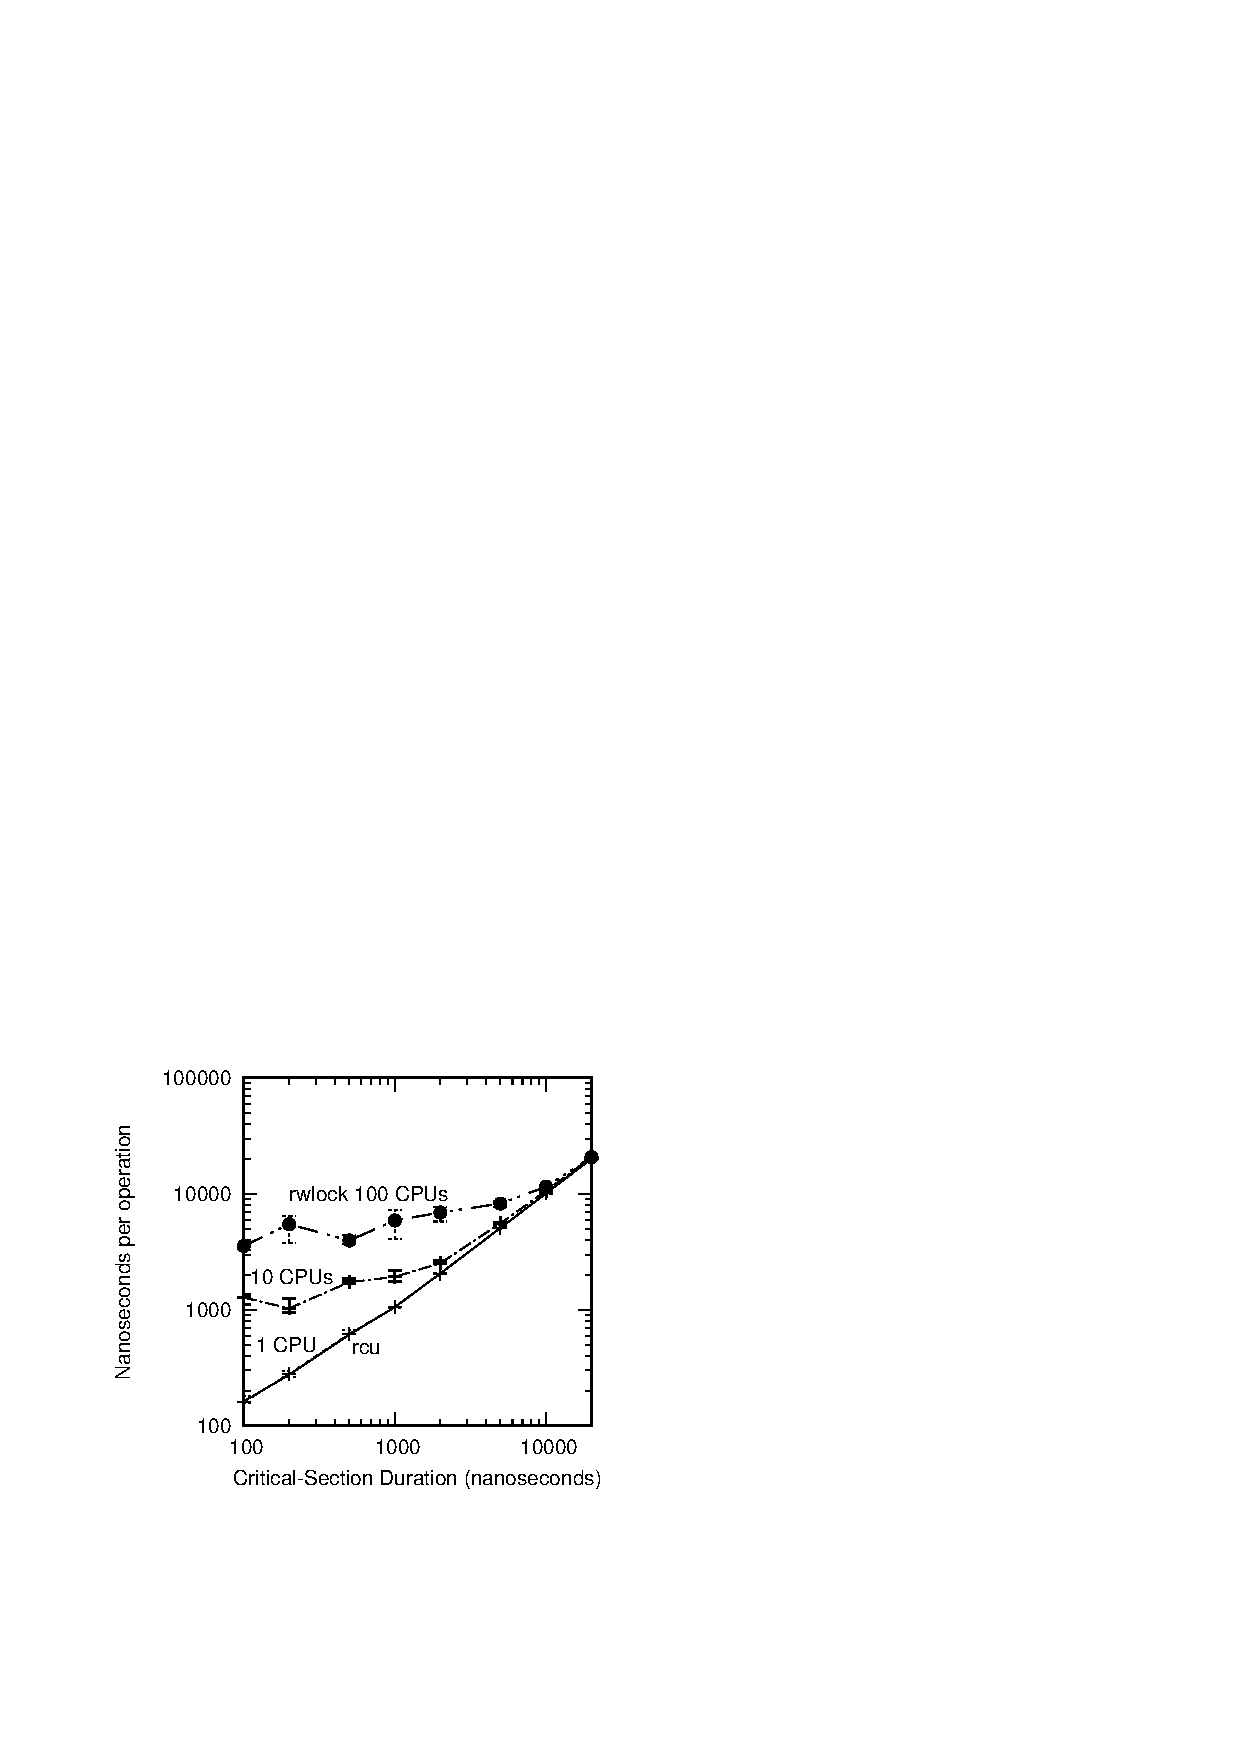
\includegraphics{defer/rwlockRCUperfwt}}
\caption{Comparison of RCU to Reader-Writer Locking as Function of Critical-Section Duration, 192 CPUs}
\label{fig:defer:Comparison of RCU to Reader-Writer Locking as Function of Critical-Section Duration}
\end{figure}

물론,
\cref{fig:defer:Performance Advantage of RCU Over Reader-Writer Locking,%
fig:defer:Performance Advantage of Preemptible RCU Over Reader-Writer Locking}
의 reader-writer 락킹의 낮은 성능은 비현실적인 0의 길이를 갖는 크리티컬 섹션에
의해 과장된 것입니다.
RCU 의 성능 이득은 크리티컬 섹션의 길이가 길어질수록 줄어듭니다.
이런 감소가 앞의 그림과 같은 시스템에서 수행된
Figure~\ref{fig:defer:Comparison of RCU to Reader-Writer Locking as Function of Critical-Section Duration}
에 보여져 있습니다.
여기서, y 축은 read-side 기능의 오버헤드와 크리티컬 섹션의 오버헤드의 합을, x
축은 크리티컬 섹션의 오버헤드를 나노세컨드 단위로 표현합니다.
하지만 y 축이 로그스케일이어서 이 그림에서의 작은 차이가 여전히 상당한 차이를
표현함을 기억해 두시기 바랍니다.
이 그림은 non-preemptible RCU 를 보입니다만, preemptible RCU 의 read-side
오버헤드가 3 나노세컨드란 점을 놓고 보면, 그 그림은
Figure~\ref{fig:defer:Comparison of RCU to Reader-Writer Locking as Function of Critical-Section Duration}
와 거의 같을 겁니다.

\iffalse

Of course, the low performance of reader-writer locking in
\cref{fig:defer:Performance Advantage of RCU Over Reader-Writer Locking,%
fig:defer:Performance Advantage of Preemptible RCU Over Reader-Writer Locking}
is exaggerated by the unrealistic zero-length critical sections.
The performance advantages of RCU decrease as the overhead of the critical
sections increase.
This decrease can be seen in
Figure~\ref{fig:defer:Comparison of RCU to Reader-Writer Locking as Function of Critical-Section Duration},
which was run on the same system as the previous plots.
Here, the y-axis represents the sum of the overhead of the read-side
primitives and that of the critical section and the x-axis represents
the critical-section overhead in nanoseconds.
But please note the logscale y~axis, which means that the small
separations between the traces still represent significant differences.
This figure shows non-preemptible RCU, but given that preemptible RCU's
read-side overhead is only about three nanoseconds, its plot would be
nearly identical to
Figure~\ref{fig:defer:Comparison of RCU to Reader-Writer Locking as Function of Critical-Section Duration}.

\fi

\QuickQuiz{
	Figure~\ref{fig:defer:Comparison of RCU to Reader-Writer Locking as Function of Critical-Section Duration}
	의 마이크로세컨드 미만 기간에서의 더 큰 에러 범위는 왜 그런거죠?

	\iffalse

	Why the larger error ranges for the submicrosecond durations in
	Figure~\ref{fig:defer:Comparison of RCU to Reader-Writer Locking as Function of Critical-Section Duration}?

	\fi

}\QuickQuizAnswer{
	더 작은 거리는 더 작은 측정에서 더 큰 상대적 에러를 초래하기
	때문입니다.
	또한, 리눅스 커널의 \co{ndelay()} 나노세컨드 단위 기능은 (2020년
	기준으로) 마이크로세컨드 이상의 시간단위 데이터를 위해 사용되는
	\co{udelay()} 보다 덜 정확합니다.
	Figure~\ref{fig:defer:Performance Advantage of RCU Over Reader-Writer Locking}
	에 보인 0 의 길이의 경우와 비교해 보는게 유익할 겁니다.

	\iffalse

	Because smaller disturbances result in greater relative errors
	for smaller measurements.
	Also, the Linux kernel's \co{ndelay()} nanosecond-scale primitive
	is (as of 2020) less accurate than is the \co{udelay()} primitive
	used for the data for durations of a microsecond or more.
	It is instructive to compare to the zero-length case shown in
	Figure~\ref{fig:defer:Performance Advantage of RCU Over Reader-Writer Locking}.

	\fi

}\QuickQuizEnd

Reader-writer 락킹을 위한 세개의 선이 있는데, 위의 것은 100~CPU, 그
다음은 10~CPU, 그리고 아래의 것은 1~CPU 에서의 것입니다.
따라서 CPU 의 수가 커지고 크리티컬 섹션이 짧아질수록 RCU 의 성능 이득은
커집니다.
이런 성능 이득은 100-CPU 시스템이 더이상 드물지 않고 여러 시스템 콜이 (그리고
그것들이 내포하는 RCU read-side 크리티컬 섹션이) 마이크로세컨드 내에 완료된다는
사실에 의해 과소평가되었습니다.

첨언하자면, 다음 문단에서 이야기 되듯, RCU read-side 기능은 거의 완전히
데드락에 내성을 가지고 있습니다.

\iffalse

There are three traces for reader-writer locking, with the upper trace
being for 100~CPUs, the next for 10~CPUs, and the lowest for 1~CPU\@.
So the greater the number of CPUs and the shorter the critical sections,
the greater is RCU's performance advantage.
These performance advantages are underscored by the fact that 100-CPU
systems are no longer uncommon and that a number of system calls (and
thus any RCU read-side critical sections that they contain) complete
within a microsecond.

In addition, as is discussed in the next paragraph,
RCU read-side primitives are almost entirely deadlock-immune.

\fi


\paragraph{Deadlock Immunity}

RCU 가 읽기가 대부분인 워크로드에 상당한 성능 이득을 제공하지만, RCU 를 만든
주요 이유는 사실 그것의 read-side 데드락 내성을 위함이었습니다.
이 내성은 RCU read-side 기능이 블록하거나 스핀하거나 뒤쪽으로 브랜칭하지 않아서
그 수행시간이 정해져있다는 사실에서 기인합니다.
따라서 그것들은 데드락 사이클에 참여될 수가 없습니다.

\iffalse

Although RCU offers significant performance advantages for
read-mostly workloads, one of the primary reasons for creating
RCU in the first place was in fact its immunity to read-side
deadlocks.
This immunity stems from the fact that
RCU read-side primitives do not block, spin, or even
do backwards branches, so that their execution time is deterministic.
It is therefore impossible for them to participate in a deadlock
cycle.

\fi

\QuickQuiz{
	이 데드락 내성에 예외가 있나요?  만약 그렇다면 어떤 이벤트들의 연속이
	데드락을 이르게 할 수 있나요?

	\iffalse

	Is there an exception to this deadlock immunity, and if so,
	what sequence of events could lead to deadlock?

	\fi

}\QuickQuizAnswer{
	RCU read-side 기능이 관여된 데드락 사이클을 만드는 한가지 방법은 다음의
	(불법적인) 선언문의 연속입니다:

	\iffalse

	One way to cause a deadlock cycle involving
	RCU read-side primitives is via the following (illegal) sequence
	of statements:

	\fi

\begin{VerbatimU}
rcu_read_lock();
synchronize_rcu();
rcu_read_unlock();
\end{VerbatimU}

	이 \co{synchronize_rcu()} 는 앞서서부터 존재한 모든 RCU read-side
	크리티컬 섹션이 완료되기 전까지 리턴할 수 없지만,
	\co{synchronize_rcu()} 가 리턴하기 전까지는 완료될 수 없는 RCU
	read-side 크리티컬 섹션에 감싸여 있습니다.
	그 결과는 고전적인 스스로에 대한 데드락입니다---reader-writer 락의
	경우에도 읽기 락을 쥐고 있는 상태에서 쓰기 락을 쥐려고 시도하면 똑같은
	결과를 얻을 겁니다.

	이 스스로에 대한 데드락 시나리오는 RCU QSBR 에 적용되지 않는데,
	\co{synchronize_rcu()} 에 의해 수행되는 컨텍스트 스위치는 이 CPU 를
	위한 quiescent state 로 동작하여 grace period 가 종료되게 할 것이기
	때문임을 알아두시기 바랍니다.
	하지만, 이는 심지어 더 나쁜 것일 뿐일텐데, 이 RCU read-side 크리티컬
	섹션에 의해 사용되는 데이터는 이 grace period 완료로 인해 메모리
	해제되었을 수도 있기 때문입니다.

	요약하자면,
	\cref{tab:defer:RCU Wait-to-Finish APIs} 에 나열된
	synchronous RCU update-side 기능을 RCU read-side 크리티컬 섹션 내에서
	사용하지 마십시오.

	\iffalse

	The \co{synchronize_rcu()} cannot return until all
	pre-existing RCU read-side critical sections complete, but
	is enclosed in an RCU read-side critical section that cannot
	complete until the \co{synchronize_rcu()} returns.
	The result is a classic self-deadlock---you get the same
	effect when attempting to write-acquire a reader-writer lock
	while read-holding it.

	Note that this self-deadlock scenario does not apply to
	RCU QSBR, because the context switch performed by the
	\co{synchronize_rcu()} would act as a quiescent state
	for this CPU, allowing a grace period to complete.
	However, this is if anything even worse, because data used
	by the RCU read-side critical section might be freed as a
	result of the grace period completing.

	In short, do not invoke synchronous RCU update-side primitives, which
	are listed in
	\cref{tab:defer:RCU Wait-to-Finish APIs},
	from within an RCU read-side critical section.

	\fi

}\QuickQuizEnd

RCU 의 read-side 데드락 내성의 한가지 흥미로운 결론은 RCU 읽기 쓰레드를
무조건적으로 RCU 업데이트 쓰레드로 업그레이드 할 수 있다는 것입니다.
Reader-writer 락킹에서 그런 업그레이드를 시도하는 것은 데드락을 초래합니다.
RCU read-to-update 업그레이드를 하는 코드 조각은 다음과 같을겁니다:

\iffalse

An interesting consequence of RCU's read-side deadlock immunity is
that it is possible to unconditionally upgrade an RCU
reader to an RCU updater.
Attempting to do such an upgrade with reader-writer locking results
in deadlock.
A sample code fragment that does an RCU read-to-update upgrade follows:

\fi

\begin{VerbatimN}[samepage=true]
rcu_read_lock();
list_for_each_entry_rcu(p, &head, list_field) {
	do_something_with(p);
	if (need_update(p)) {
		spin_lock(my_lock);
		do_update(p);
		spin_unlock(&my_lock);
	}
}
rcu_read_unlock();
\end{VerbatimN}

\co{do_update()} 는 락의 보호, \emph{그리고} RCU read-side 보호 아래 수행됨에
주의하십시오.

RCU 의 데드락 내성의 또다른 흥미로운 결론은 커다란 범주의 우선순위 역전 문제에
대한 내성입니다.
예를 들어, 낮은 우선순위 RCU 읽기 쓰레드가 높은 우선순위 RCU 업데이트 쓰레드가
update-side 락을 잡는걸 방지하지 못합니다.
비슷하게, 낮은 우선순위 RCU 업데이트 쓰레드는 높은 우선순위 RCU 읽기 쓰레드가
RCU read-side 크리티컬 섹션에 들어가는 것을 막지 못합니다.

\iffalse

Note that \co{do_update()} is executed under
the protection of the lock \emph{and} under RCU read-side protection.

Another interesting consequence of RCU's deadlock immunity is its
immunity to a large class of priority inversion problems.
For example, low-priority RCU readers cannot prevent a high-priority
RCU updater from acquiring the update-side lock.
Similarly, a low-priority RCU updater cannot prevent high-priority
RCU readers from entering an RCU read-side critical section.

\fi

\QuickQuiz{
	데드락과 우선순위 역전에 모두 내성이 있다???
	사실이라기엔 너무 좋아보이는데요.
	이게 가능하다는 걸 제가 왜 믿어야 하죠?

	\iffalse

	Immunity to both deadlock and priority inversion???
	Sounds too good to be true.
	Why should I believe that this is even possible?

	\fi

}\QuickQuizAnswer{
	진짜 동작합니다.
	어쨌건, 그렇지 않다면 리눅스 커널은 동작하지 못할겁니다.

	\iffalse

	It really does work.
	After all, if it didn't work, the Linux kernel would not run.

	\fi

}\QuickQuizEnd

\paragraph{Realtime Latency}

RCU read-side 기능들은 스핀하지도 블록하지도 않기 때문에, 훌륭한 realtime
반응시간을 제공합니다.
추가적으로, 앞에서도 이야기 했듯 이는 RCU read-side 기능들과 락이 연관된
우선순위 역전 문제에 내성이 있음을 의미합니다.

하지만, RCU 는 더 복잡한 우선순위 역전 시나리오에는 문제가 있을 수 있는데, 예를
들면 높은 우선순위의 프로세스는 낮은 우선순위의 RCU 읽기 쓰레드에 의해 \rt\
커널에서 한 RCU grace period 가 지나갈 때까지 블록될 수 있습니다.
이는 RCU 우선순위 부스팅을 통해 해결될 수
있습니다~\cite{PaulEMcKenney2007BoostRCU,DinakarGuniguntala2008IBMSysJ}.

\iffalse

Because RCU read-side primitives neither spin nor block, they offer
excellent realtime latencies.
In addition, as noted earlier, this means that they are
immune to priority inversion
involving the RCU read-side primitives and locks.

However, RCU is susceptible to more subtle priority-inversion scenarios,
for example, a high-priority process blocked waiting for an RCU
grace period to elapse can be blocked by low-priority RCU readers
in \rt\ kernels.
This can be solved by using RCU priority
boosting~\cite{PaulEMcKenney2007BoostRCU,DinakarGuniguntala2008IBMSysJ}.

\fi

\paragraph{RCU Readers and Updaters Run Concurrently}

RCU 읽기 쓰레드는 스핀도 블록도 하지 않으므로, 그리고 업데이트 쓰레드는 어떤
종류의 롤백이나 abort 도 하지 않으므로, RCU 읽기 쓰레드와 업데이트 쓰레드는
동시에 수행되어야만 합니다.
이는 RCU 읽기 쓰레드가 오래되어 더이상 유효하지 않은 데이터를 읽을수도 있고,
비일관적인 모습을 보게 될수도 있음을, 따라서 reader-writer 락킹에서 RCU 로의
전환에 혼란을 야기할 수 있음을 의미합니다.

\iffalse

Because RCU readers never spin nor block, and because updaters are not
subject to any sort of rollback or abort semantics, RCU readers and
updaters must necessarily run concurrently.
This means that RCU readers might access stale data, and might even
see inconsistencies, either of which can render conversion from reader-writer
locking to RCU non-trivial.

\fi

\begin{figure}[tb]
\centering
\resizebox{3in}{!}{\includegraphics{defer/rwlockRCUupdate}}
\caption{Response Time of RCU vs. Reader-Writer Locking}
\label{fig:defer:Response Time of RCU vs. Reader-Writer Locking}
\end{figure}

하지만, 놀라우리만치 많은 상황에서 비일관성과 오래되어 더이상 유효하지 않은
데이터는 문제가 되지 않습니다.
고전적인 예는 네트워킹 라우팅 테이블입니다.
라우팅 업데이트는 특정 시스템까지 닿는데 상당한 시간을 요하므로 (수초에서
수분까지도), 시스템은 이 업데이트가 도착하기 전까지 상당한 시간동안 패킷을
잘못된 방향으로 보낼 수 있습니다.
업데이트를 몇 추가적인 밀리세컨드 동안 잘못된 방향으로 보내는 건 보통 문제가
아닙니다.
더 나아가, RCU 업데이트 쓰레드는 RCU 읽기 쓰레드가 끝나기를 기다리지 않고
변화를 만들 수 있으므로, RCU 읽기 쓰레드는
Figure~\ref{fig:defer:Response Time of RCU vs. Reader-Writer Locking}
에 보인 것처럼 batch-fair reader-writer 락킹의 읽기 쓰레드보다 빠르게 변화를 볼
수도 있습니다.

\iffalse

However, in a surprisingly large number of situations, inconsistencies and
stale data are not problems.
The classic example is the networking routing table.
Because routing updates can take considerable time to reach a given
system (seconds or even minutes), the system will have been sending
packets the wrong way for quite some time when the update arrives.
It is usually not a problem to continue sending updates the wrong
way for a few additional milliseconds.
Furthermore, because RCU updaters can make changes without waiting for
RCU readers to finish,
the RCU readers might well see the change more quickly than would
batch-fair
reader-writer-locking readers, as shown in
Figure~\ref{fig:defer:Response Time of RCU vs. Reader-Writer Locking}.

\fi

일단 업데이트가 도달하면, rwlock 쓰기 쓰레드는 마지막 읽기 쓰레드가 완료되기
전까지 진행될 수 없으며, 뒤따르는 읽기 쓰레드는 이 쓰기 쓰레드가 완료되기
전까지 진행될 수 없습니다.
하지만, 이 뒤따르는 읽기 쓰레드는 오른쪽 상자의 초록색으로 표시되었듯 이 새
값을 읽을 수 있는게 보장됩니다.
대조적으로, RCU 읽기 쓰레드와 업데이트 쓰레드는 서로를 블록할 수 없어서, RCU
읽기 쓰레드가 이 업데이트된 값을 더 빨리 볼 수 있게 합니다.
물론, 이것들의 수행이 RCU 업데이트 쓰레드의 그것과 겹치므로, \emph{모든} RCU
읽기 쓰레드는 업데이트된 값을 읽을 수도 있는데, 이 업데이트 전부터 시작된
세개의 읽기 쓰레드 역시 포함됩니다.
하지만 초록색으로 칠해진 가장 오른쪽 RCU 읽기 쓰레드만이 업데이트된 값을 볼
것으로 \emph{보장됩니다}.

Reader-writer 락킹과 RCU 는 그저 다른 보장을 제공할 뿐입니다.
Reader-writer 락킹에서 어떤 쓰기 쓰레드의 시작보다 나중에 시작된 읽기 쓰레드는
새 값을 볼 것이 보장되고, 이 쓰레드가 스핀하고 있는 사이 시작되려 하는 읽기
쓰레드는 새 값을 볼수도 보지 못할 수도 있는데, 사용되는 rwlock 구현의 읽기/쓰기
쓰레드 선호도에 의존적입니다.
대조적으로, RCU 에서 업데이트 쓰레드가 완료되기 전에 시작된 모든 읽기 쓰레드는
새 값을 볼 것이 보장되며, 업데이트 쓰레드가 시작한 후에 완료된 모든 읽기
쓰레드는 타이밍에 따라 새 값을 볼 수도 보지 못할 수도 있습니다.

\iffalse

Once the update is received, the rwlock writer cannot proceed until the
last reader completes, and subsequent readers cannot proceed until the
writer completes.
However, these subsequent readers are guaranteed to see the new value,
as indicated by the green shading of the rightmost boxes.
In contrast, RCU readers and updaters do not block each other, which permits
the RCU readers to see the updated values sooner.
Of course, because their execution overlaps that of the RCU updater,
\emph{all} of the RCU readers might well see updated values, including
the three readers that started before the update.
Nevertheless only the green-shaded rightmost RCU readers
are \emph{guaranteed} to see the updated values.

Reader-writer locking and RCU simply provide different guarantees.
With reader-writer locking, any reader that begins after the writer begins
is guaranteed to see new values, and any reader that attempts to
begin while the writer is spinning might or might not see new values,
depending on the reader/writer preference of the rwlock implementation in
question.
In contrast, with RCU, any reader that begins after the updater completes
is guaranteed to see new values, and any reader that completes after the
updater begins might or might not see new values, depending on timing.

\fi

여기서의 핵심은 reader-writer 락킹이 컴퓨터 시스템 내에서는 일관성을 실제로
보장하지만, 이 일관성이 바깥 세상의 \emph{비일관성} 의 증가를 대가로 오는
경우가 존재한다는 것입니다.
달리 말하자면 reader-writer 락킹은 바깥 세상 관점에서 조용하게 오래되어
유효하지 않아진 데이터를 대가로 내부적 일관성을 획득합니다.

그러나, 시스템 내에서의 비일관성과 오래되어 유효하지 않아진 데이터가 제어되지
못하는 상황도 있습니다.
다행히, 비일관성과 오래되어 유효하지 않아진 데이터를 막는 여러 방법이
존재하며~\cite{PaulEdwardMcKenneyPhD,Arcangeli03}, 레퍼런스 카운팅에 기반한
일부 방법이 Section~\ref{sec:defer:Reference Counting} 에서 다루어집니다.

\iffalse

The key point here is that, although reader-writer locking does
indeed guarantee consistency within the confines of the computer system,
there are situations where this consistency comes at the price of
increased \emph{inconsistency} with the outside world.
In other words, reader-writer locking obtains internal consistency at the
price of silently stale data with respect to the outside world.

Nevertheless, there are situations where inconsistency and stale
data within the confines of the system cannot be tolerated.
Fortunately,
there are a number of approaches that avoid inconsistency and stale
data~\cite{PaulEdwardMcKenneyPhD,Arcangeli03}, and some
methods based on reference counting are discussed in
Section~\ref{sec:defer:Reference Counting}.

\fi

\paragraph{Low-Priority RCU Readers Can Block High-Priority Reclaimers}

Realtime RCU~\cite{DinakarGuniguntala2008IBMSysJ} 또는
SRCU~\cite{PaulEMcKenney2006c} 에서, preemption 당한 읽기 쓰레드는 grace period
가 완료되는 것을 막을 것인데, 심지어 높은 우선순위 작업이 그 grace period
완료를 기다리며 블록되어 있더라도 그렇습니다.
Realtime RCU 는 \co{call_rcu()} 로 \co{synchronize_rcu()} 를 대체하거나 RCU
우선순위 부스팅을
이용해~\cite{PaulEMcKenney2007BoostRCU,DinakarGuniguntala2008IBMSysJ} 이를 막을
수 있는데, 2008년 초 기준으로 아직 실험적 상태입니다.
SRCU 와 QRCU 를 우선순위 부스팅과 결합시키는게 필요해질 수도 있지만, 분명한
실제 세계에서의 필요가 확인되기 전까지는 아닙니다.

\iffalse

In Realtime RCU~\cite{DinakarGuniguntala2008IBMSysJ} or
SRCU~\cite{PaulEMcKenney2006c},
a preempted reader will prevent a grace period from completing, even if
a high-priority task is blocked waiting for that grace period to complete.
Realtime RCU can avoid this problem by substituting \co{call_rcu()}
for \co{synchronize_rcu()} or by using RCU priority
boosting~\cite{PaulEMcKenney2007BoostRCU,DinakarGuniguntala2008IBMSysJ},
which is still in experimental status as of early 2008.
It might become necessary to augment SRCU and QRCU with priority boosting,
but not before a clear real-world need is demonstrated.

\fi

\paragraph{RCU Grace Periods Extend for Many Milliseconds}

Userspace RCU~\cite{MathieuDesnoyers2009URCU,PaulMcKenney2013LWNURCU}, 가속된
grace period, 그리고
Appendix~\ref{chp:app:``Toy'' RCU Implementations} 에 이야기 된 여러 ``장난감''
RCU 구현들의 예외가 있지만, RCU grace period 는 수 밀리세컨드까지 늘어날 수
있습니다.
가능한 곳에 비동기 인터페이스를 (\co{call_rcu()} 와 \co{call_rcu_bh()})
사용하는 것을 포함해 그런 오랜 지연을 문제가 되지 않게 하는 여러 기법이
존재하지만 이는 RCU 가 읽기가 대부분인 상황에서 사용되는 관습적 규칙의 주요
이유 중 하나입니다.

\iffalse

With the exception of userspace
RCU~\cite{MathieuDesnoyers2009URCU,PaulMcKenney2013LWNURCU},
expedited grace periods, and several of the ``toy''
RCU implementations described in
Appendix~\ref{chp:app:``Toy'' RCU Implementations},
RCU grace periods extend milliseconds.
Although there are a number of techniques to render such long delays
harmless, including use of the asynchronous interfaces where available
(\co{call_rcu()} and \co{call_rcu_bh()}), this situation
is a major reason for the rule of thumb that RCU be used in read-mostly
situations.

\fi

\paragraph{Code: Reader-Writer Locking vs. RCU Code}

최선의 경우, reader-writer 락킹에서 RCU 로의 전환은
Listing~\ref{lst:defer:Converting Reader-Writer Locking to RCU: Data},
\ref{lst:defer:Converting Reader-Writer Locking to RCU: Search},
그리고
\ref{lst:defer:Converting Reader-Writer Locking to RCU: Deletion}
에 보인 것처럼 상당히 단순할 수 있는데, 이것들은 모두
Wikipedia~\cite{WikipediaRCU} 에서 가져온 것들입니다.

\iffalse


In the best case, the conversion from reader-writer locking to RCU
is quite simple, as shown in
Listings~\ref{lst:defer:Converting Reader-Writer Locking to RCU: Data},
\ref{lst:defer:Converting Reader-Writer Locking to RCU: Search},
and
\ref{lst:defer:Converting Reader-Writer Locking to RCU: Deletion},
all taken from
Wikipedia~\cite{WikipediaRCU}.

\fi

\begin{listing*}[htbp]
{ \scriptsize
\begin{verbbox}
 1 struct el {                           1 struct el {
 2   struct list_head lp;                2   struct list_head lp;
 3   long key;                           3   long key;
 4   spinlock_t mutex;                   4   spinlock_t mutex;
 5   int data;                           5   int data;
 6   /* Other data fields */             6   /* Other data fields */
 7 };                                    7 };
 8 DEFINE_RWLOCK(listmutex);             8 DEFINE_SPINLOCK(listmutex);
 9 LIST_HEAD(head);                      9 LIST_HEAD(head);
\end{verbbox}
}
\hspace*{0.9in}\OneColumnHSpace{-0.5in}
\theverbbox
\caption{Converting Reader-Writer Locking to RCU: Data}
\label{lst:defer:Converting Reader-Writer Locking to RCU: Data}
\end{listing*}

\begin{listing*}[htbp]
{ \scriptsize
\begin{verbbox}
 1 int search(long key, int *result)     1 int search(long key, int *result)
 2 {                                     2 {
 3   struct el *p;                       3   struct el *p;
 4                                       4
 5   read_lock(&listmutex);              5   rcu_read_lock();
 6   list_for_each_entry(p, &head, lp) { 6   list_for_each_entry_rcu(p, &head, lp) {
 7     if (p->key == key) {              7     if (p->key == key) {
 8       *result = p->data;              8       *result = p->data;
 9       read_unlock(&listmutex);        9       rcu_read_unlock();
10       return 1;                      10       return 1;
11     }                                11     }
12   }                                  12   }
13   read_unlock(&listmutex);           13   rcu_read_unlock();
14   return 0;                          14   return 0;
15 }                                    15 }
\end{verbbox}
}
\hspace*{0.9in}\OneColumnHSpace{-0.5in}
\theverbbox
\caption{Converting Reader-Writer Locking to RCU: Search}
\label{lst:defer:Converting Reader-Writer Locking to RCU: Search}
\end{listing*}

\begin{listing*}[htbp]
{ \scriptsize
\begin{verbbox}
 1 int delete(long key)                  1 int delete(long key)
 2 {                                     2 {
 3   struct el *p;                       3   struct el *p;
 4                                       4
 5   write_lock(&listmutex);             5   spin_lock(&listmutex);
 6   list_for_each_entry(p, &head, lp) { 6   list_for_each_entry(p, &head, lp) {
 7     if (p->key == key) {              7     if (p->key == key) {
 8       list_del(&p->lp);               8       list_del_rcu(&p->lp);
 9       write_unlock(&listmutex);       9       spin_unlock(&listmutex);
                                        10       synchronize_rcu();
10       kfree(p);                      11       kfree(p);
11       return 1;                      12       return 1;
12     }                                13     }
13   }                                  14   }
14   write_unlock(&listmutex);          15   spin_unlock(&listmutex);
15   return 0;                          16   return 0;
16 }                                    17 }
\end{verbbox}
}
\hspace*{0.9in}\OneColumnHSpace{-0.5in}
\theverbbox
\caption{Converting Reader-Writer Locking to RCU: Deletion}
\label{lst:defer:Converting Reader-Writer Locking to RCU: Deletion}
\end{listing*}

하지만, 이런 전환이 항상 단순하지는 않습니다.
이는
\cref{lst:defer:Converting Reader-Writer Locking to RCU: Deletion}
의 \co{spin_lock()} 도 \co{synchronize_rcu()} 도
\cref{lst:defer:Converting Reader-Writer Locking to RCU: Search}
의 읽기 쓰레드를 배제시키지 않기 때문입니다.
첫째로, \co{spin_lock()} 은 \co{rcu_read_lock()} 과 \co{rcu_read_unlock()} 과
상호작용하지 않으며 따라서 그것들을 배제하지 않습니다.
둘째로, \co{write_lock()} 과 \co{synchronize_rcu()} 가 앞서서부터 존재한 읽기
쓰레드를 기다리지만 \co{write_lock()} 만이 뒤따르는 읽기 쓰레드의 시작을
방지합니다.\footnote{
	누구였든 이걸 Paul 에게 지적해준 분에게 감사를.}
따라서, \co{synchronize_rcu()} 는 읽기 쓰레드를 배제하지 못합니다.
따라서 reader-writer 락킹을 사용하는 많은 상황이 RCU 로 쉽게 바뀔 수 있다는
사실은 놀랍습니다.

Reader-writer 락킹을 RCU 로 교체하는 더 자세한 경우들이 다른 곳에서도 발견될 수
있을 겁니다~\cite{NeilBrown2015PathnameLookup,NeilBrown2015RCUwalk}.

\iffalse

However, the transformation is not always this straightforward.
This is because neither the \co{spin_lock()} nor the
\co{synchronize_rcu()} in
\cref{lst:defer:Converting Reader-Writer Locking to RCU: Deletion}
exclude the readers in
\cref{lst:defer:Converting Reader-Writer Locking to RCU: Search}.
First, the \co{spin_lock()} does not interact in any way with
\co{rcu_read_lock()} and \co{rcu_read_unlock()}, thus not excluding them.
Second, although both \co{write_lock()} and \co{synchronize_rcu()}
wait for pre-existing readers, only \co{write_lock()} prevents
subsequent readers from commencing.\footnote{
	Kudos to whoever pointed this out to Paul.}
Thus, \co{synchronize_rcu()} cannot exclude readers.
It is therefore surprising that a great many situations
using reader-writer locking can be easily converted to RCU\@.

More-elaborate cases of replacing reader-writer locking with RCU
may be found
elsewhere~\cite{NeilBrown2015PathnameLookup,NeilBrown2015RCUwalk}.

\fi

\paragraph{Semantics: Reader-Writer Locking vs. RCU Semantics}

Reader-writer 락킹 semantic 은 거칠고 비정규적으로 다음의 세가지 임시적 제약으로
요약될 수 있습니다:

\begin{enumerate}
\item	쓰기 락 획득은 모든 읽기 락을 잡은 쓰레드들이 그 락을 놓기를
	기다립니다.
\item	쓰기 락 획득은 모든 쓰기 락을 잡은 쓰레드들이 그 락을 놓기를
	기다립니다.
\item	읽기 락 획득은 모든 쓰기 락을 잡은 쓰레드들이 그 락을 놓기를
	기다립니다.
\end{enumerate}

\iffalse

Reader-writer locking semantics can be roughly and informally summarized
by the following three temporal constraints:

\begin{enumerate}
\item	Write-side acquisitions wait for any read-holders to release
	the lock.
\item	Writer-side acquisitions wait for any write-holder to release
	the lock.
\item	Read-side acquisitions wait for any write-holder to release
	the lock.
\end{enumerate}

\fi

RCU 는 제약~\#3 을 완전히 사라지게 하고 나머지 두개도 다음과 같이 완화시킵니다:

\begin{enumerate}
\item	쓰기 쓰레드는 모든 앞서서부터 존재해온 읽기 락을 잡은 쓰레드들을
	업데이트의 파괴적인 단계를 (일반적으로 메모리 해제) 처리하기 전에
	기다립니다.
\item	쓰기 쓰레드는 서로간에 필요한 바에 맞춰 동기화 합니다.
\end{enumerate}

물론 이 완화가 RCU 구현이 훌륭한 성능과 확장성을 얻을 수 있게 합니다.
RCU 사용처들은 이 완화를 놀랄만큼 많은 방법으로 보상합니다만 일반적으로 공간적
제약을 사용합니다:

\begin{enumerate}
\item	새 데이터는 새로 할당된 메모리에 위치합니다.
\item	오래된 데이터는 메모리 해제되지만, 다음의 조건이 충족된 후에만 합니다:
	\begin{enumerate}
	\item	데이터가 뒤의 읽기 쓰레드에 의해선 접근 불가능하게끔 링크
		삭제되었을 것, 그리고
	\item	뒤따르는 RCU grace period 가 지났을 것.
	\end{enumerate}
\end{enumerate}

\iffalse

RCU dispenses entirely with constraint~\#3 and weakens the other two
as follows:

\begin{enumerate}
\item	Writers wait for any pre-existing read-holders before progressing
	to the destructive phase of their update (usually the freeing of
	memory).
\item	Writers synchronize with each other as needed.
\end{enumerate}

It is of course this weakening that permits RCU implementations to attain
excellent performance and scalability.
RCU use cases compensate for this weakening in a surprisingly large number
of ways, but most commonly by imposing spatial constraints:

\begin{enumerate}
\item	New data is placed in newly allocated memory.
\item	Old data is freed, but only after:
	\begin{enumerate}
	\item	That data has been unlinked so as to be inaccessible
		to later readers, and
	\item	A subsequent RCU grace period has elapsed.
	\end{enumerate}
\end{enumerate}

\fi

요약해서, RCU 는 자신의 쓰기 성능과 확장성을 시공간적 제약에 기반한 semantic 을
통해 얻습니다.

\iffalse

In short, RCU attains its read-side performance and scalability by
constructing semantics based on combined temporal and spatial constraints.

\fi

\subsubsection{RCU is a Restricted Reference-Counting Mechanism}
\label{sec:defer:RCU is a Restricted Reference-Counting Mechanism}

Grace period 는 진행중인 RCU read-side 크리티컬 섹션이 있는 동안은 완료될 수
없으므로, RCU read-side 기능들은 제한된 레퍼런스 카운팅 메커니즘으로 사용될 수
있습니다.
예를 들어, 다음 코드 조각을 생각해 봅시다:

\iffalse

Because grace periods are not allowed to complete while
there is an RCU read-side critical section in progress,
the RCU read-side primitives may be used as a restricted
reference-counting mechanism.
For example, consider the following code fragment:

\fi

\begin{VerbatimN}
rcu_read_lock();  /* acquire reference. */
p = rcu_dereference(head);
/* do something with p. */
rcu_read_unlock();  /* release reference. */
\end{VerbatimN}

\co{rcu_read_lock()} 기능은 \co{p} 로의 레퍼런스를 얻는 것으로 생각될 수도
있는데, \co{rcu_dereference()} 가 \co{p} 에 값을 할당한 뒤에 시작되는 grace
period 는 우리가 매칭되는 \co{rcu_read_unlock()} 전까지는 종료될 수 없기
때문입니다.
이 레퍼런스 카운팅 방법은 우리가 RCU read-side 크리티컬 섹션 내에서는 블록될 수
없으며 RCU read-side 크리티컬 섹션을 한 태스크에서 다른 태스크로 넘길 수도
없다는 사실로 제약이 됩니다.

이런 제약과 무관하게, 다음 코드는 안전하게 \co{p} 를 삭제합니다:

\iffalse

The \co{rcu_read_lock()} primitive can be thought of as
acquiring a reference to \co{p}, because a grace period
starting after the \co{rcu_dereference()} assigns to \co{p}
cannot possibly end until after we reach the matching
\co{rcu_read_unlock()}.
This reference-counting scheme is restricted in that
we are not allowed to block in RCU read-side critical sections,
nor are we permitted to hand off an RCU read-side critical section
from one task to another.

Regardless of these restrictions,
the following code can safely delete \co{p}:

\fi

\begin{VerbatimN}
spin_lock(&mylock);
p = head;
rcu_assign_pointer(head, NULL);
spin_unlock(&mylock);
/* Wait for all references to be released. */
synchronize_rcu();
kfree(p);
\end{VerbatimN}

\co{head} 로의 할당은 미래의 \co{p} 로의 레퍼런스가 얻어지는 것을 방지하고,
\co{synchronize_rcu()} 는 모든 앞서 획득된 레퍼런스가 해제되기를 기다립니다.

\iffalse

The assignment to \co{head} prevents any future references
to \co{p} from being acquired, and the \co{synchronize_rcu()}
waits for any previously acquired references to be released.

\fi

\QuickQuiz{
	하지만 잠시만요!
	이건 RCU 를 reader-writer 락킹의 대체제로 생각할 때 사용될 수 있는 것과
	완전히 똑같은 코드예요!
	뭐죠?

	\iffalse

	But wait!
	This is exactly the same code that might be used when thinking
	of RCU as a replacement for reader-writer locking!
	What gives?

	\fi

}\QuickQuizAnswer{
	이건 장난감 예제의 법칙의 효과입니다:
	어떤 지점 이후부터는 코드 조각들은 똑같이 보입니다.
	유일한 차이점은 우리가 그 코드를 어떻게 생각하느냐에 있습니다.
	하지만, 이 차이점은 무척 중요할 수 있습니다.
	그 중요성에 대해 한가지만 예를 들어보자면, 우리가 RCU 를 제한된
	레퍼런스 카운팅 방법으로 생각한다면, 우린 업데이트가 RCU read-side
	크리티컬 섹션을 배제시킬 거라는 바보스러운 생각에 빠지진 않을 겁니다.

	그러나 RCU 를 reader-writer 락킹의 대체제로 생각하는 것도 종종
	유용한데, 예를 들면 reader-writer 락킹을 RCU 로 대체할 때 그렇습니다.

	\iffalse

	This is an effect of the Law of Toy Examples:
	beyond a certain point, the code fragments look the same.
	The only difference is in how we think about the code.
	However, this difference can be extremely important.
	For but one example of the importance, consider that if we think
	of RCU as a restricted reference counting scheme, we would never
	be fooled into thinking that the updates would exclude the RCU
	read-side critical sections.

	It nevertheless is often useful to think of RCU as a replacement
	for reader-writer locking, for example, when you are replacing
	reader-writer locking with RCU\@.

	\fi

}\QuickQuizEnd

물론, RCU 는
Section~\ref{sec:together:Refurbish Reference Counting}
에서 이야기 된 것처럼 전통적인 레퍼런스 카운팅과 결합될 수도 있습니다.

\iffalse

Of course, RCU can also be combined with traditional reference counting,
as discussed in
Section~\ref{sec:together:Refurbish Reference Counting}.

\fi

\begin{figure}[tb]
\centering
\resizebox{2.5in}{!}{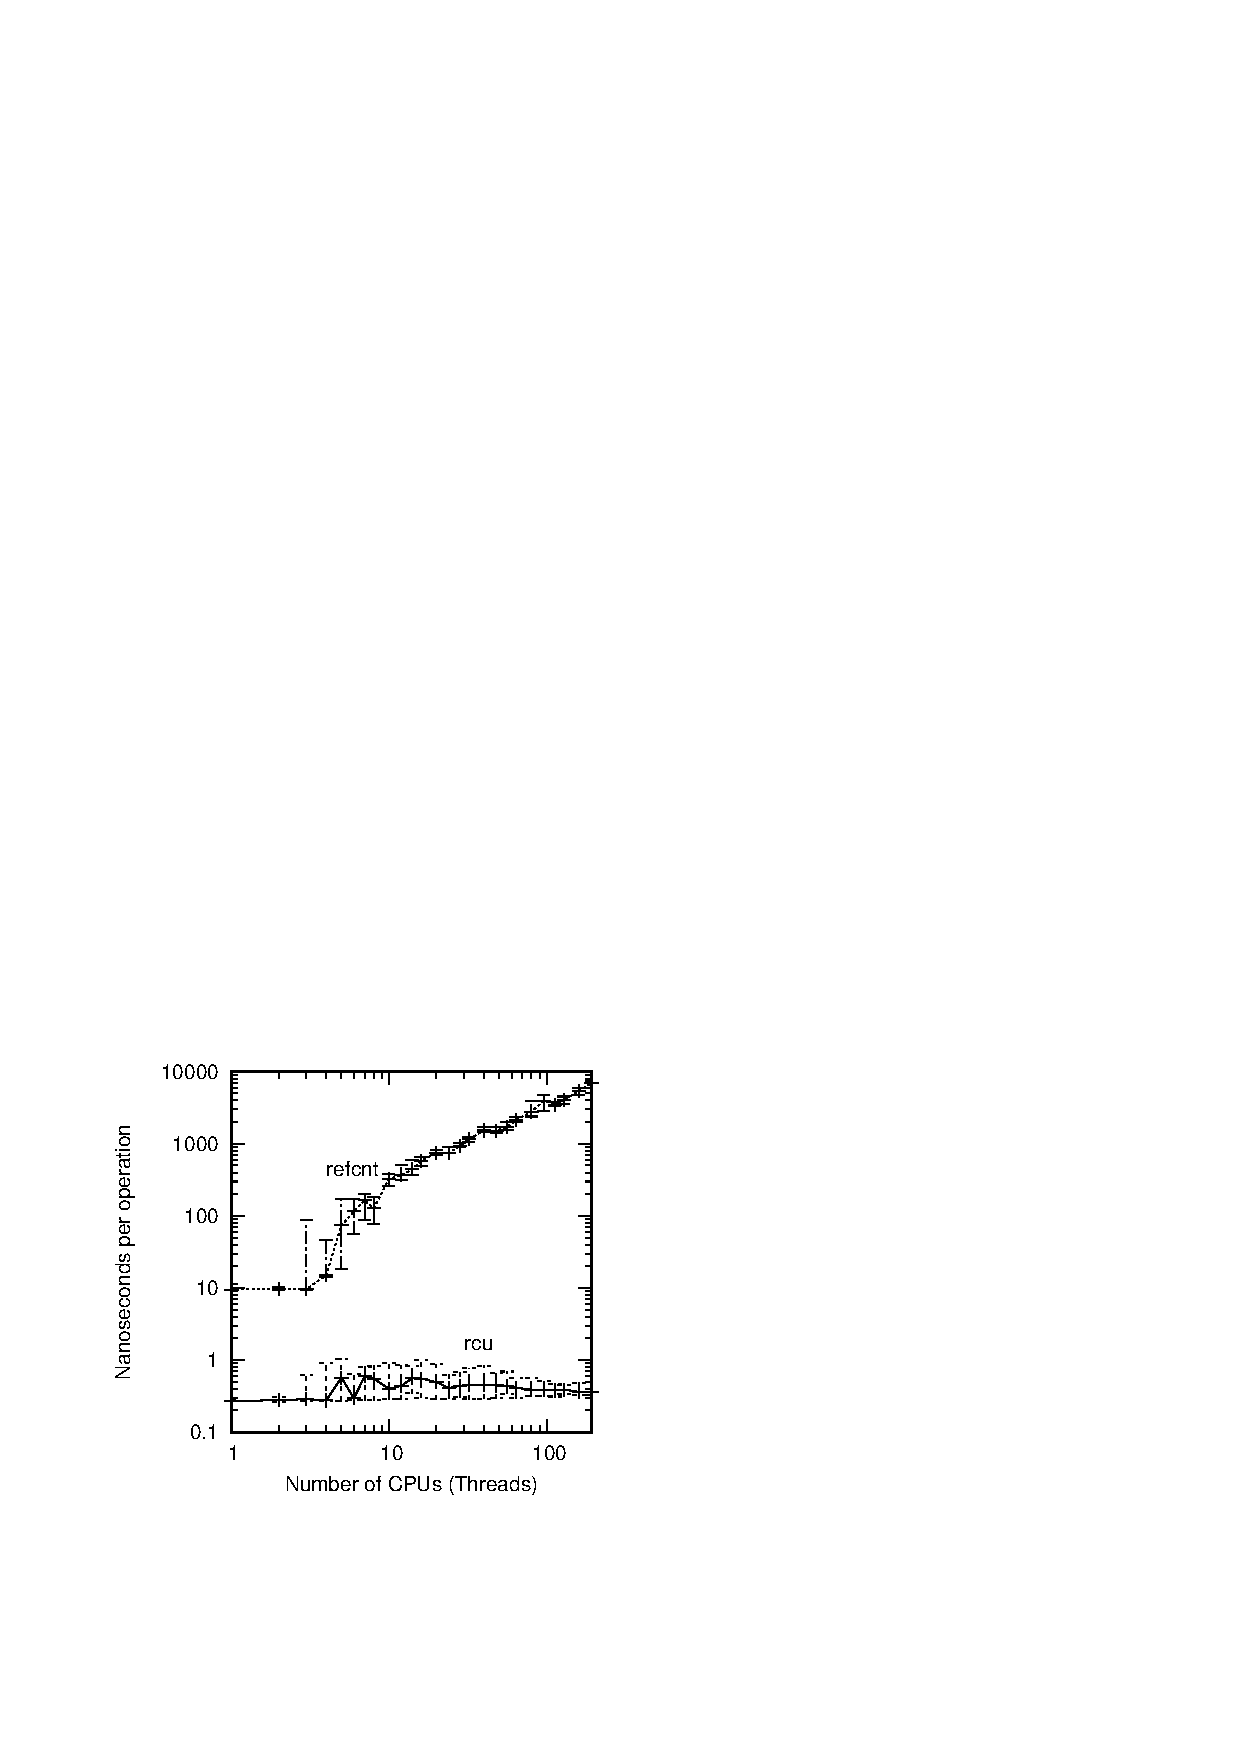
\includegraphics{defer/refcntRCUperf}}
\caption{Performance of RCU vs. Reference Counting}
\label{fig:defer:Performance of RCU vs. Reference Counting}
\end{figure}

\begin{figure}[tb]
\centering
\resizebox{2.5in}{!}{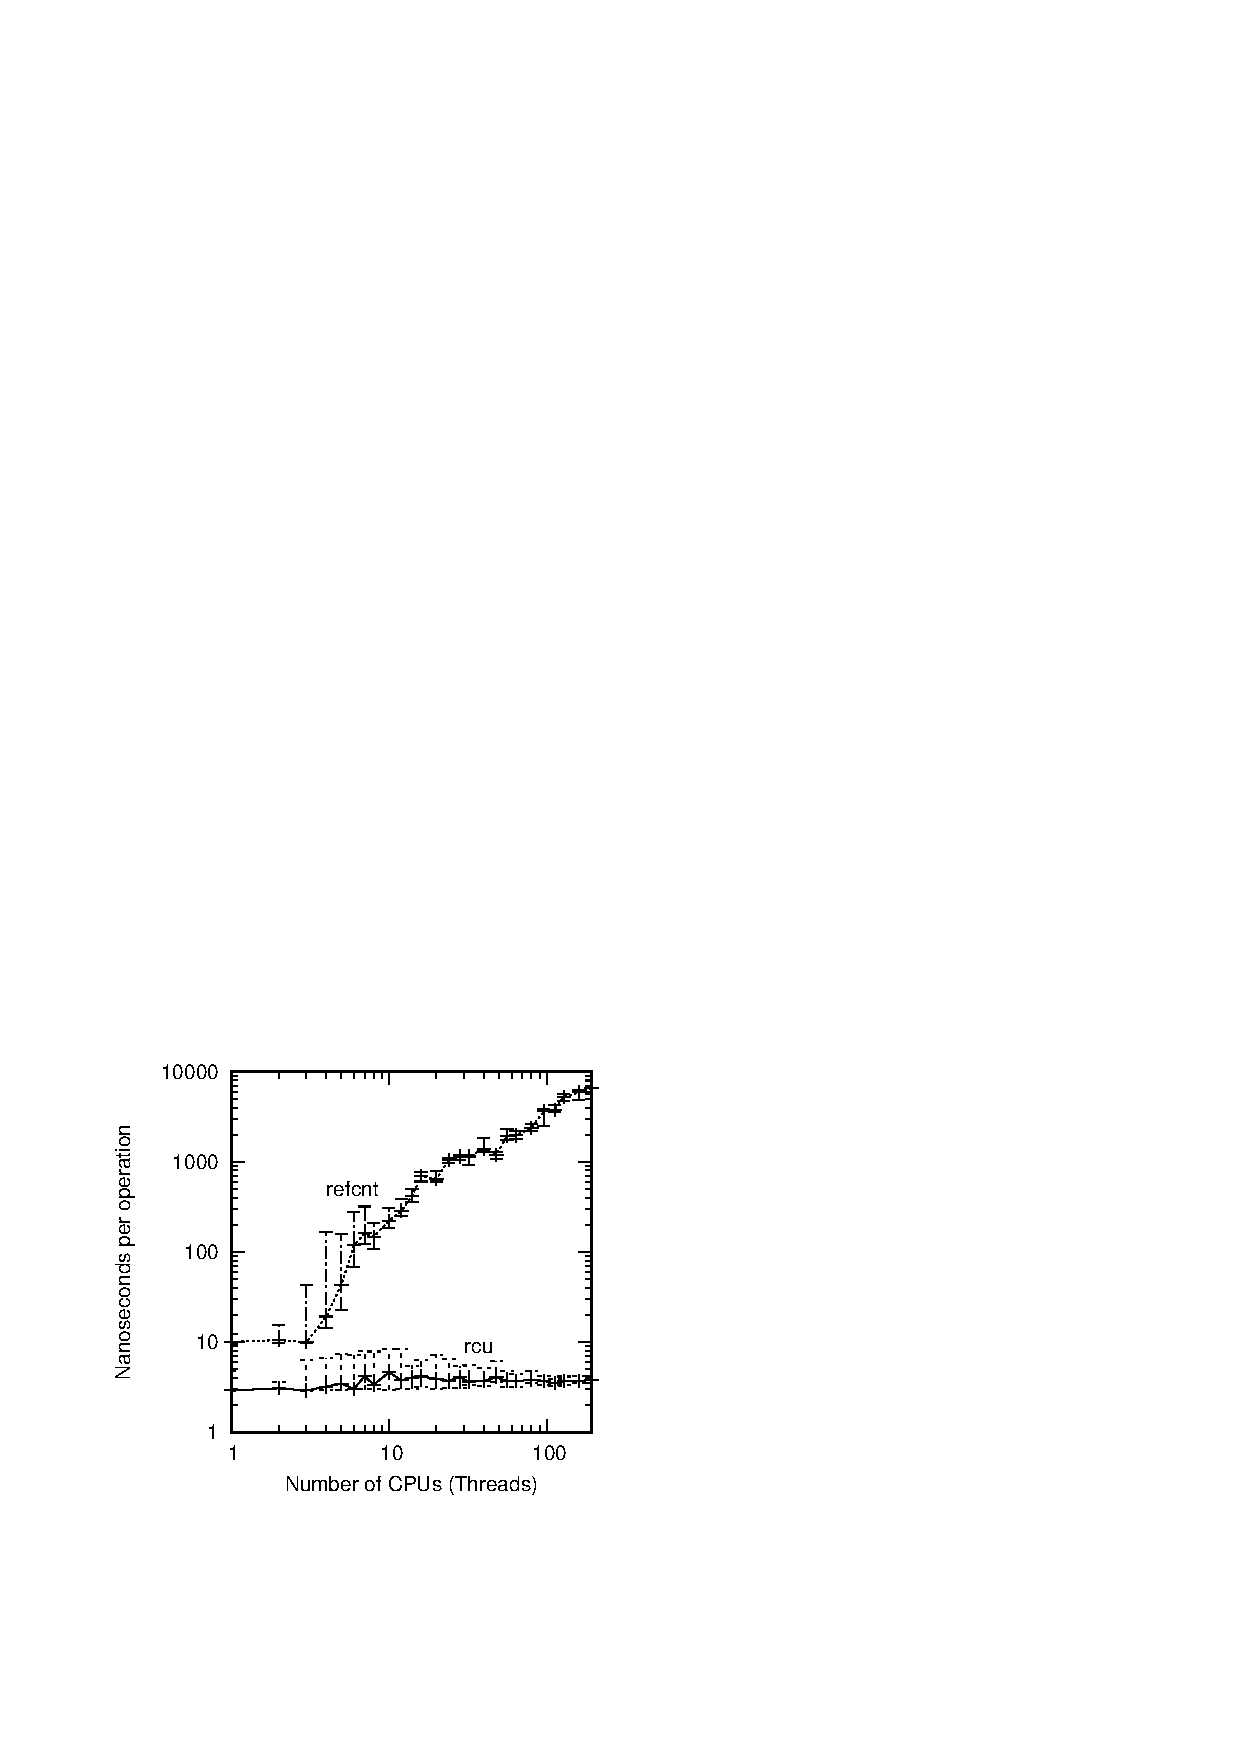
\includegraphics{defer/refRCUperfPREEMPT}}
\caption{Performance of Preemptible RCU vs. Reference Counting}
\label{fig:defer:Performance of Preemptible RCU vs. Reference Counting}
\end{figure}

그런데 이걸 왜 신경씁니까?
다시 말하지만, 답은 성능으로, 448-CPU 2.1\,GHz Intel x86 시스템에서
non-preemptible 과 preemtible 리눅스 커널 RCU 를 사용해 각각 얻어진
Figure~\ref{fig:defer:Performance of RCU vs. Reference Counting}
와~\ref{fig:defer:Performance of Preemptible RCU vs. Reference Counting}
에서 보인 것과 같습니다.
Non-preemptible RCU 의 레퍼런스 카운팅 대비 장점은 단일 CPU 에서 수십배를
넘으며 192~CPU 에서는 수만배까지 달합니다.
Preemptible RCU 의 장점은 단일 CPU 에서 약 세배에서 192~CPU 에서 수천배까지
이릅니다.

\iffalse

But why bother?
Again, part of the answer is performance, as shown in
Figures~\ref{fig:defer:Performance of RCU vs. Reference Counting}
and~\ref{fig:defer:Performance of Preemptible RCU vs. Reference Counting},
again showing data taken on a 448-CPU 2.1\,GHz Intel x86 system
for non-preemptible and preemptible Linux-kernel RCU, respectively.
Non-preemptible RCU's advantage over reference counting ranges from
more than an order of magnitude at one CPU up to about four orders of
magnitude at 192~CPUs.
Preemptible RCU's advantage ranges from about a factor of three at
one CPU up to about three orders of magnitude at 192~CPUs.

\fi

\begin{figure}[tb]
\centering
\resizebox{2.5in}{!}{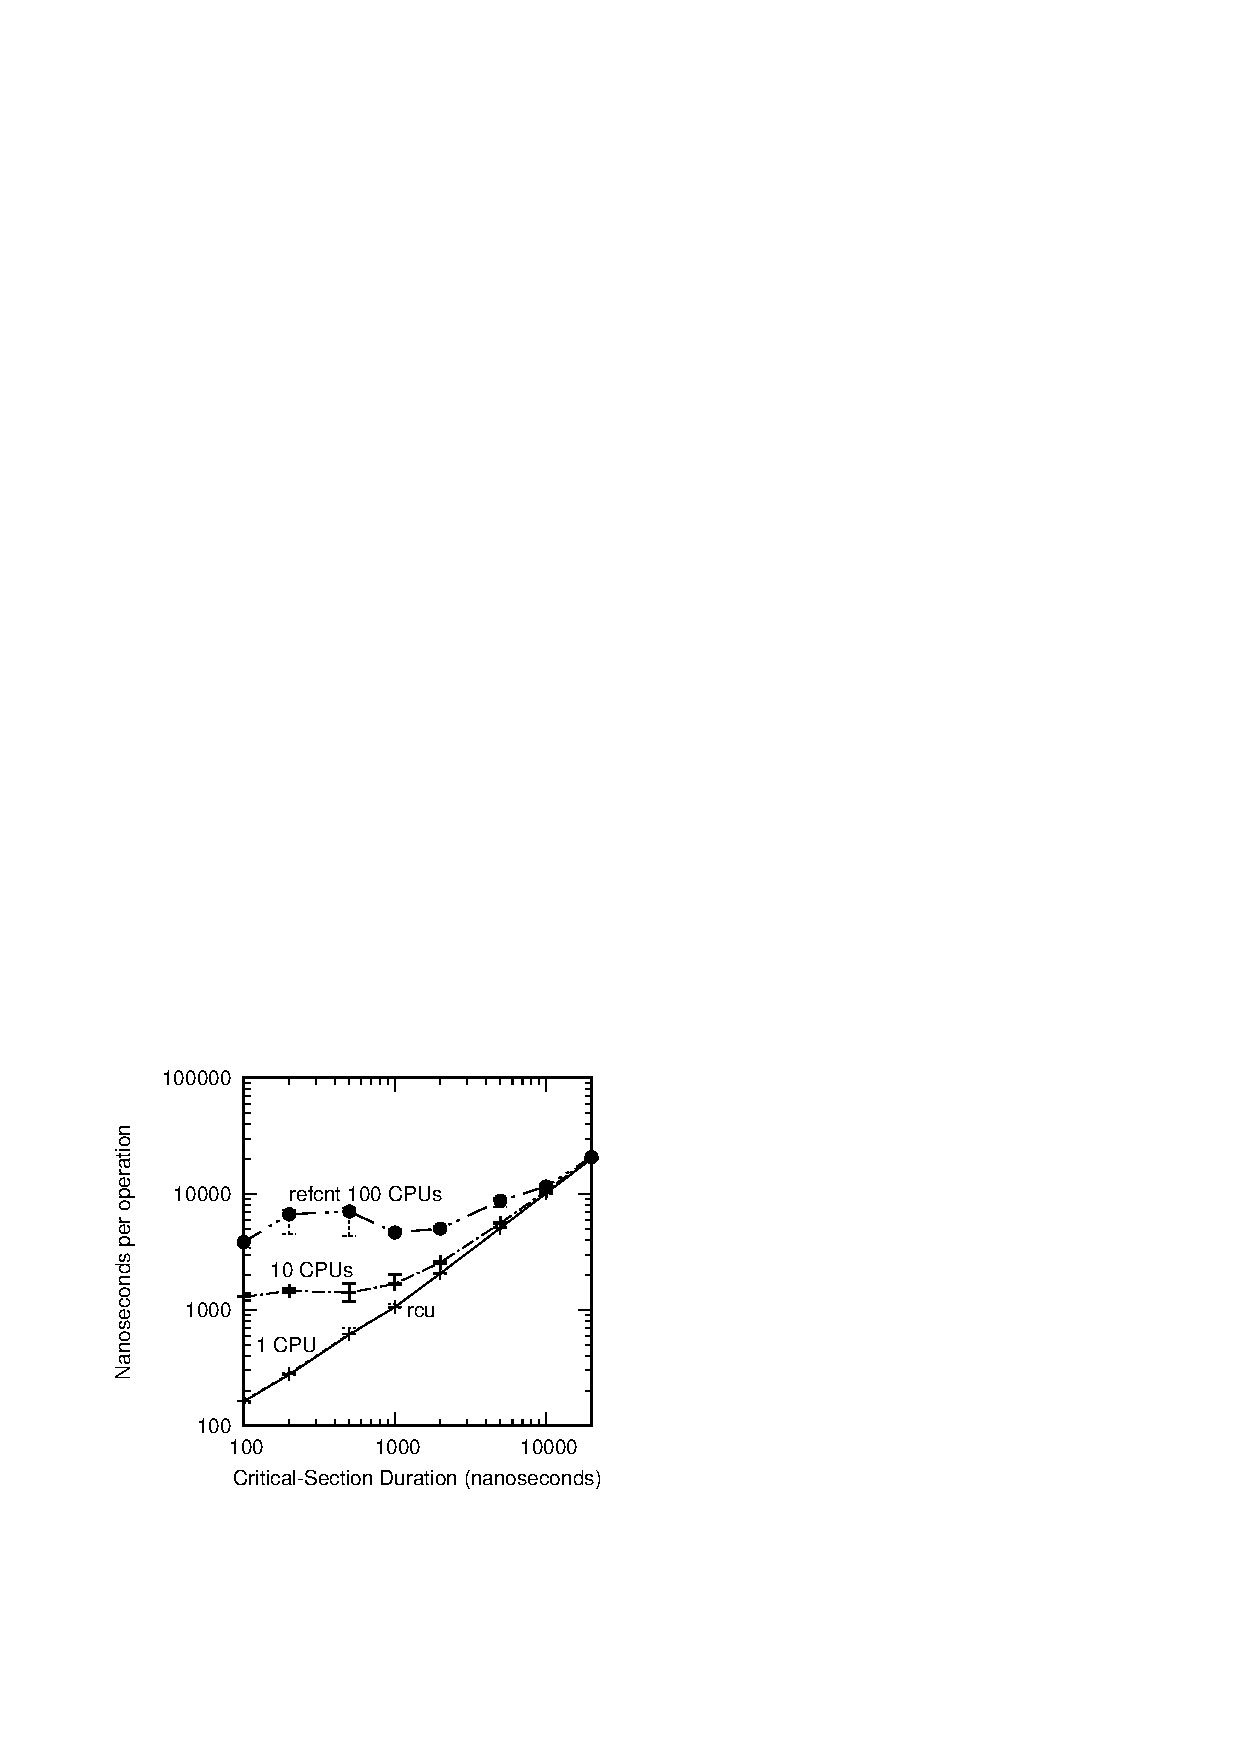
\includegraphics{defer/refRCUperfwt}}
\caption{Response Time of RCU vs. Reference Counting, 192 CPUs}
\label{fig:defer:Response Time of RCU vs. Reference Counting}
\end{figure}

하지만, reader-writer 락킹에서와 같이, RCU 의 이 성능 이득은 같은 시스템에서
Figure~\ref{fig:defer:Response Time of RCU vs. Reference Counting}
에 보인 것처럼 대부분 큰 수의 CPU 와 짧은 기간의 크리티컬 섹션으로부터
나왔습니다.
더해서, reader-writer 락킹에서와 같이, 많은 시스템 콜은 (그리고 따라서 그것들이
포함하는 모든 RCU read-side 크리티컬 섹션은) 수 마이크로세컨드 내에 완료됩니다.

그러나, RCU 에 의해 발생하는 제약들은 상당히 귀찮을 수 있습니다.
예를 들어, 많은 경우, RCU read-side 크리티컬 섹션 내에서의 잠자는 것의 금지는
그 목표를 의미없게 할 수도 있습니다.
다음 섹션은 이 문제를 해결하는 동시에 적어도 일부 경우에서는 전통적 레퍼런스
카운팅의 복잡도를 줄이는 방법들을 살펴봅니다.\footnote{
	다른 경우들은 \cref{sec:defer:Hazard Pointers} 에서 설명된 해저드
	포인터 메커니즘을 통해 더 잘 처리될 수도 있습니다.}

\iffalse

However, as with reader-writer locking, the performance advantages of
RCU are most pronounced for short-duration critical sections and for
large numbers of CPUs, as shown in
Figure~\ref{fig:defer:Response Time of RCU vs. Reference Counting}
for the same system.
In addition, as with reader-writer locking, many system calls (and thus
any RCU read-side critical sections that they contain) complete in
a few microseconds.

However, the restrictions that go with RCU can be quite onerous.
For example, in many cases, the prohibition against sleeping while in an RCU
read-side critical section would defeat the entire purpose.
The next section looks at ways of addressing this problem, while also
reducing the complexity of traditional reference counting, at least in
some cases.\footnote{
	Other cases might be better served by the hazard pointers
	mechanism described in \cref{sec:defer:Hazard Pointers}.}

\fi

\subsubsection{RCU is a Bulk Reference-Counting Mechanism}
\label{sec:defer:RCU is a Bulk Reference-Counting Mechanism}

앞의 섹션에서 이야기 되었듯, 전통적 레퍼런스 카운터는 일반적으로 특정 데이터
구조, 또는 특정 데이터 구조체들의 그룹과 연관지어집니다.
하지만, 단일한 글로벌 레퍼런스 카운터를 다양한 데이터 구조를 위해 유지하는 것은
보통 이 레퍼런스 카운트를 포함하는 캐쉬 라인이 이리저리 이동되게 합니다.
그런 캐쉬 라인 움직임은 성능을 상당히 떨어뜨릴 수 있습니다.

대조적으로, RCU 의 가벼운 read-side 기능은 무시 가능한 수준의 성능 하락과 함께
극단적으로 빈번한 read-side 사용을 가능하게 하여 RCU 가 약간 또는 없는 성능
하락을 갖는 ``bulk 레퍼런스 카운팅'' 으로 사용될 수 있게 합니다.
블록되어야 하는 코드 섹션을 가로질러 단일 태스크를 통해 레퍼런스가 얻어져야만
하는 상황에서는 Sleepable RCU (SRCU)~\cite{PaulEMcKenney2006c} 가 사용될 수
있을 겁니다.
이는 레퍼런스가 한 태스크에서 다른 태스크로 ``전달되는'', 예를 들면 어떤
레퍼런스가 I/O 시작 시에 획득되고 연관된 완료 인터럽트 핸들러에서 해제되는 것과
같은 드물지는 않은 상황은 처리할 수 없을 겁니다.
(원칙적으로, 이는 SRCU 구현에 의해 처리될 수 있습니다만, 실질적으로는 이게 좋은
트레이드오프인지 아직 명확치 않습니다.)

\iffalse

As noted in the preceding section,
traditional reference counters are usually associated with a specific
data structure, or perhaps a specific group of data structures.
However, maintaining a single global reference counter for a large
variety of data structures typically results in bouncing
the cache line containing the reference count.
Such cache-line bouncing can severely degrade performance.

In contrast, RCU's lightweight read-side primitives permit
extremely frequent read-side usage with negligible performance
degradation, permitting RCU to be used as a ``bulk reference-counting''
mechanism with little or no performance penalty.
Situations where a reference must be held by a single task across a
section of code that blocks may be accommodated with
Sleepable RCU (SRCU)~\cite{PaulEMcKenney2006c}.
This fails to cover the not-uncommon situation where a reference is ``passed''
from one task to another, for example, when a reference is acquired
when starting an I/O and released in the corresponding completion
interrupt handler.
(In principle, this could be handled by the SRCU implementation,
but in practice, it is not yet clear whether this is a good tradeoff.)

\fi

물론, SRCU 는 그 자체의 제약을 가지는데, \co{srcu_read_lock()} 에서 리턴된 값이
연관된 \co{srcu_read_unlock()} 에 전달되어야 하며, 어떤 SRCU 기능도 하드웨어
인터럽트 핸들러나 non-maskable 인터럽트 (NMI) 핸들러에서 수행되어선 안된다는
것입니다.
이 제약에 의해 얼마나 많은 문제가 있는지, 그것들이 어떻게 처리되는 것이
최선인지에 대해선 아직 판단 중입니다.

\iffalse

Of course, SRCU brings restrictions of its own, namely that the
return value from \co{srcu_read_lock()} be passed into the
corresponding \co{srcu_read_unlock()}, and that no SRCU primitives
be invoked from hardware interrupt handlers or from non-maskable interrupt
(NMI) handlers.
The jury is still out as to how much of a problem is presented by
these restrictions, and as to how they can best be handled.

\fi

\subsubsection{RCU is a Poor Man's Garbage Collector}
\label{sec:defer:RCU is a Poor Man's Garbage Collector}

RCU 를 처음 배우는 사람들의 드물지 않은 느낌은 ``RCU 는 가비지 콜렉터 같은
거다!'' 입니다.
이 느낌은 상당한 사실을 담고 있지만, 잘못된 생각의 방향을 갖게 될수도 있습니다.

RCU 와 자동화된 가비지 콜레터 (GC) 사이의 관계에 대해 생각하는 최선의 방법은
RCU 는 GC 를  쓰레기를 모으는 \emph{타이밍} 을 자동으로 결정해 준다는 점에서
닮았다는 것이겠습니다만, RCU 는 GC 와 다음과 같은 점에서 다릅니다:
(1)~프로그래머는 일일이 언제 특정 데이터 구조가 정리될 수 있는지 알려야 하며,
(2)~프로그래머는 일일이 데이터가 참조되고 있을 수도 있는 RCU read-side 크리티컬
섹션을 표시해야 합니다.

이 차이점에도 불구하고, 닮은 부분도 꽤 깊습니다.
실제로, 제가 알고 있는 첫번째 RCU와 비슷한 메커니즘의 사용은 grace period 를
제어하기 위한 레퍼런스 카운트 기반 가비지 콜렉터~\cite{Kung80} 였으며, RCU 와
가비지 콜렉터 사이의 연결은 더 최근에도 이야기
되었습니다~\cite{HarshalSheth2016goRCU}.
그러나, RCU 를 생각하는 더 나은 방법이 다음 섹션에 설명되어 있습니다.

\iffalse

A not-uncommon exclamation made by people first learning about
RCU is ``RCU is sort of like a garbage collector!''
This exclamation has a large grain of truth, but it can also be
misleading.

Perhaps the best way to think of the relationship between RCU
and automatic garbage collectors (GCs) is that RCU resembles
a GC in that the \emph{timing} of collection is automatically
determined, but that RCU differs from a GC in that: (1)~the programmer
must manually indicate when a given data structure is eligible
to be collected, and (2)~the programmer must manually mark the
RCU read-side critical sections where references might be held.

Despite these differences, the resemblance does go quite deep.
In fact, the first RCU-like mechanism I am aware of used a
reference-count-based garbage collector to handle the grace
periods~\cite{Kung80}, and the connection between RCU and
garbage collection has been noted more
recently~\cite{HarshalSheth2016goRCU}.
Nevertheless, a better way of thinking of RCU is described in the
following section.

\fi

\subsubsection{RCU is an MVCC}
\label{sec:defer:RCU is an MVCC}

RCU 는 또한 단순화 된, 완화된 일관성 기준을 갖는 multi-version concurrency
contro (MVCC) 메커니즘으로 생각될 수 있습니다.
이 멀티 버전 이야기는
\cref{sec:defer:Maintain Multiple Versions of Recently Updated Objects}
에서 다루어진 바 있습니다.
하지만, 그 기본적 형태에서, RCU 는 버전 일관성을 특정 RCU 로 보호되는 데이터
원소에 대해서만 제공합니다.

그러나, 더 높은 단계에서의 버전 일관성을 복구하기 위한 여러 기법이 사용될 수
있는데, 예를 들면equence locking 을 사용하거나
(\cref{sec:together:Correlated Data Elements} 를 참고하세요)
추가적인 우회 방법을 사용하는 겁니다
(\cref{sec:together:Correlated Fields} 를 참고하세요).

\iffalse

RCU can also be thought of as a simplified multi-version concurrency
control (MVCC) mechanism with weak consistency criteria.
The multi-version aspects were touched upon in
\cref{sec:defer:Maintain Multiple Versions of Recently Updated Objects}.
However, in its native form, RCU provides version consistency only
within a given RCU-protected data element.

However, a number of techniques can be used to restore version consistency
at a higher level, for example, using sequence locking
(see \cref{sec:together:Correlated Data Elements})
or imposing additional levels of indirection
(see \cref{sec:together:Correlated Fields}).

\fi

\subsubsection{RCU Provides Existence Guarantees}
\label{sec:defer:RCU Provides Existence Guarantees}

Gamsa 등은~\cite{Gamsa99} 존재 보장에 대해 논하고 RCU 를 닮은 어떤 메커니즘이
어떻게 이런 존재 보장을 제공하기 위해 사용될 수 있는지 설명하며 (해당 PDF 의
페이지~7 의 Section~5 를 보세요),
Section~\ref{sec:locking:Lock-Based Existence Guarantees}
은 락킹을 사용해 어떻게 존재 보장을 할 수 있는지를 그렇게 하는 것의 단점과 함께
설명합니다.
그 효과는 어떤 RCU 로 보호되는 데이터 원소든 하나의 RCU read-side 크리티컬 섹션
내에서 액세스 된다면, 그 데이터 원소는 해당 RCU read-side 크리티컬 섹션의 기간
동안은 존재하는 것이 보장된다는 것입니다.

\iffalse

Gamsa et al.~\cite{Gamsa99}
discuss existence guarantees and describe how a mechanism
resembling RCU can be used to provide these existence guarantees
(see Section~5 on page~7 of the PDF), and
Section~\ref{sec:locking:Lock-Based Existence Guarantees}
discusses how to guarantee existence via locking, along with the
ensuing disadvantages of doing so.
The effect is that if any RCU-protected data element is accessed
within an RCU read-side critical section, that data element is
guaranteed to remain in existence for the duration of that RCU
read-side critical section.

\fi

\begin{listing}[tbp]
\begin{fcvlabel}[ln:defer:Existence Guarantees Enable Per-Element Locking]
\begin{VerbatimL}[commandchars=\\\@\$]
int delete(int key)
{
	struct element *p;
	int b;

	b = hashfunction(key);			\lnlbl@hash$
	rcu_read_lock();			\lnlbl@rdlock$
	p = rcu_dereference(hashtable[b]);
	if (p == NULL || p->key != key) {	\lnlbl@chkkey$
		rcu_read_unlock();		\lnlbl@rdunlock1$
		return 0;			\lnlbl@ret_0:a$
	}
	spin_lock(&p->lock);			\lnlbl@acq$
	if (hashtable[b] == p && p->key == key) {\lnlbl@chkkey2$
		rcu_read_unlock();		\lnlbl@rdunlock2$
		rcu_assign_pointer(hashtable[b], NULL);\lnlbl@remove$
		spin_unlock(&p->lock);		\lnlbl@rel1$
		synchronize_rcu();		\lnlbl@sync_rcu$
		kfree(p);			\lnlbl@kfree$
		return 1;			\lnlbl@ret_1$
	}
	spin_unlock(&p->lock);			\lnlbl@rel2$
	rcu_read_unlock();			\lnlbl@rdunlock3$
	return 0;				\lnlbl@ret_0:b$
}
\end{VerbatimL}
\end{fcvlabel}
\caption{Existence Guarantees Enable Per-Element Locking}
\label{lst:defer:Existence Guarantees Enable Per-Element Locking}
\end{listing}

\begin{fcvref}[ln:defer:Existence Guarantees Enable Per-Element Locking]
Listing~\ref{lst:defer:Existence Guarantees Enable Per-Element Locking}
은 어떻게 RCU 기반의 존재 보장이 원소별 락킹을 가능하게 하는지 해쉬 테이블에서
원소 하나를 제거하는 함수를 통해 보입니다.
라인~\lnref{hash} 는 해쉬 함수를 계산하고, 라인~\lnref{rdlock} 은 RCU read-side
크리티컬 섹션에 진입합니다.
라인~\lnref{chkkey} 가 이 해쉬 테이블의 연관된 버킷이 비었거나 거기 있는 원소가
우리가 삭제하고자 하는 것이 아님을 발견하면, 라인~\lnref{rdunlock1} 은 RCU
read-side 크리티컬 섹션을 종료하고 라인~\lnref{ret_0:a} 에서 실패를 알립니다.
\end{fcvref}

\iffalse

\begin{fcvref}[ln:defer:Existence Guarantees Enable Per-Element Locking]
Listing~\ref{lst:defer:Existence Guarantees Enable Per-Element Locking}
demonstrates how RCU-based existence guarantees can enable
per-element locking via a function that deletes an element from
a hash table.
Line~\lnref{hash} computes a hash function, and line~\lnref{rdlock} enters an RCU
read-side critical section.
If line~\lnref{chkkey} finds that the corresponding bucket of the hash table is
empty or that the element present is not the one we wish to delete,
then line~\lnref{rdunlock1} exits the RCU read-side critical section and
line~\lnref{ret_0:a}
indicates failure.
\end{fcvref}

\fi

\QuickQuiz{
	우리가 제거하려는 원소가
	Listing~\ref{lst:defer:Existence Guarantees Enable Per-Element Locking} 의
        라인~\ref{ln:defer:Existence Guarantees Enable Per-Element Locking:chkkey}
	의 리스트의 첫번째 원소가 아니면 어떻게 되죠?

	\iffalse

	What if the element we need to delete is not the first element
	of the list on
        line~\ref{ln:defer:Existence Guarantees Enable Per-Element Locking:chkkey} of
	Listing~\ref{lst:defer:Existence Guarantees Enable Per-Element Locking}?

	\fi

}\QuickQuizAnswer{
	Listing~\ref{lst:locking:Per-Element Locking Without Existence Guarantees}
	에서와 같이, 이것은 체이닝이 없는 매우 간단한 해쉬 테이블이며, 따라서
	특정 버킷의 유일한 원소는 첫번째 원소입니다.
	독자 여러분은 다시 한번 이 예를 완전한 체이닝을 갖는 해쉬 테이블로
	조정해 보실 수 있겠습니다.
	그럴 기력이 없는 독자 분들은
	\cref{chp:Data Structures} 를 참고하고 싶으실 수도 있겠네요.

	\iffalse

	As with
	Listing~\ref{lst:locking:Per-Element Locking Without Existence Guarantees},
	this is a very simple hash table with no chaining, so the only
	element in a given bucket is the first element.
	The reader is again invited to adapt this example to a hash table with
	full chaining.
	Less energetic reader might wish to refer to
	\cref{chp:Data Structures}.

	\fi

}\QuickQuizEnd

\begin{fcvref}[ln:defer:Existence Guarantees Enable Per-Element Locking]
그렇지 않다면, 라인~\lnref{acq} 는 update-side 스핀락을 획득하고,
라인~\lnref{chkkey2} 는 이어서 이 원소가 여전히 우리가 원하는 것인지
검사합니다.
만약 그렇다면, 라인~\lnref{rdunlock2} 는 이 RCU read-side 크리티컬 섹션을
나오고, 라인~\lnref{remove} 는 이것을 테이블에서 삭제하며, 라인~\lnref{rel1}
에서 락을 해제하고, 라인~\lnref{sync_rcu} 에서 앞서서부터 존재해온 모든 RCU
read-side 크리티컬 섹션이 완료되길 기다리며, 라인~\lnref{kfree} 에서 이번에
제거된 원소를 메모리 해제하고, 라인~\lnref{ret_1} 에서 성공을 알립니다.
만약 이 원소가 더이상 우리가 원하던 것이 아니었다면, 라인~\lnref{rel2} 에서 이
락을 내려놓고, 라인~\lnref{rdunlock3} 에서 RCU read-side 크리티컬 섹션을 나온
후, 라인~\lnref{ret_0:b} 에서 이 특정 키를 제거하는데 실패했음을 알립니다.
\end{fcvref}

\iffalse

\begin{fcvref}[ln:defer:Existence Guarantees Enable Per-Element Locking]
Otherwise, line~\lnref{acq} acquires the update-side spinlock, and
line~\lnref{chkkey2} then checks that the element is still the one that we want.
If so, line~\lnref{rdunlock2} leaves the RCU read-side critical section,
line~\lnref{remove} removes it from the table, line~\lnref{rel1} releases
the lock, line~\lnref{sync_rcu} waits for all pre-existing RCU read-side critical
sections to complete, line~\lnref{kfree} frees the newly removed element,
and line~\lnref{ret_1} indicates success.
If the element is no longer the one we want, line~\lnref{rel2} releases
the lock, line~\lnref{rdunlock3} leaves the RCU read-side critical section,
and line~\lnref{ret_0:b} indicates failure to delete the specified key.
\end{fcvref}

\fi

\QuickQuizSeries{%
\QuickQuizB{
	\begin{fcvref}[ln:defer:Existence Guarantees Enable Per-Element Locking]
	Listing~\ref{lst:defer:Existence Guarantees Enable Per-Element Locking}
	의 라인~\lnref{rdunlock2} 에서는 라인\lnref{rel1} 에서 락을 내려놓기
	전에 RCU read-side 크리티컬 섹션을 빠져나가는게 왜 괜찮나요?
	\end{fcvref}

	\iffalse

	\begin{fcvref}[ln:defer:Existence Guarantees Enable Per-Element Locking]
	Why is it OK to exit the RCU read-side critical section on
	line~\lnref{rdunlock2} of
	Listing~\ref{lst:defer:Existence Guarantees Enable Per-Element Locking}
	before releasing the lock on line~\lnref{rel1}?
	\end{fcvref}

	\fi

}\QuickQuizAnswerB{
	\begin{fcvref}[ln:defer:Existence Guarantees Enable Per-Element Locking]
	첫째로, 라인~\lnref{chkkey2} 에서의 두번째 검사는 어떤 다른 CPU 가 이
	원소를 우리가 락을 획득하려 기다리는 사이에 제거했을지도 모르므로
	필요함을 알아 두시기 바랍니다.
	그러나, 우리가 이 락을 획득하는 사이 RCU read-side 크리티컬 섹션 내에
	있었다는 사실은 이 원소가 재할당되고 이 해쉬 테이블에 재삽입되었을
	가능성이 없음을 보장합니다.
	더 나아가, 일단 우리가 이 락을 획득했다면, 그 락 자체가 이 원소의
	존재를 보장하므로, 우린 더이상 이 RCU read-side 크리티컬 섹션 내에 있을
	필요가 없습니다.

	이 원소의 키를 재검사 할 필요가 있는가 하는 질문은 독자 여러분의
	연습문제로 남겨둡니다.
	\end{fcvref}

	\iffalse

	\begin{fcvref}[ln:defer:Existence Guarantees Enable Per-Element Locking]
	First, please note that the second check on line~\lnref{chkkey2} is
	necessary because some other
	CPU might have removed this element while we were waiting
	to acquire the lock.
	However, the fact that we were in an RCU read-side critical section
	while acquiring the lock guarantees that this element could not
	possibly have been re-allocated and re-inserted into this
	hash table.
	Furthermore, once we acquire the lock, the lock itself guarantees
	the element's existence, so we no longer need to be in an
	RCU read-side critical section.

	The question as to whether it is necessary to re-check the
	element's key is left as an exercise to the reader.
	% A re-check is necessary if the key can mutate or if it is
	% necessary to reject deleted entries (in cases where deletion
	% is recorded by mutating the key.
	\end{fcvref}

	\fi

}\QuickQuizEndB
%
\QuickQuizE{
	\begin{fcvref}[ln:defer:Existence Guarantees Enable Per-Element Locking]
	Listing~\ref{lst:defer:Existence Guarantees Enable Per-Element Locking}
	의 라인~\lnref{rdunlock3} 에서는 왜 라인~\lnref{rel2} 에서 락을
	내려놓기 전에 RCU read-side 크리티컬 섹션을 빠져나가지 않나요?
	\end{fcvref}

	\iffalse

	\begin{fcvref}[ln:defer:Existence Guarantees Enable Per-Element Locking]
	Why not exit the RCU read-side critical section on
	line~\lnref{rdunlock3} of
	Listing~\ref{lst:defer:Existence Guarantees Enable Per-Element Locking}
	before releasing the lock on line~\lnref{rel2}?
	\end{fcvref}

	\fi

}\QuickQuizAnswerE{
	우리가 이 두 라인의 순서를 바꾼다고 생각해 봅시다.
	그러면 이 코드는 다음 순서의 이벤트에 취약해 집니다:

	\iffalse

	Suppose we reverse the order of these two lines.
	Then this code is vulnerable to the following sequence of
	events:

	\fi

	\begin{enumerate}
	\begin{fcvref}[ln:defer:Existence Guarantees Enable Per-Element Locking]
	\item	CPU~0 가 \co{delete()} 를 호출하고, 삭제될 원소를 찾은 후,
		라인~\lnref{rdunlock2} 를 수행합니다.
		아직 원소를 삭제하지 않았지만, 곧 할겁니다.
	\item	CPU~1 이 동시에 \co{delete()} 를 호출해, 이 동일한 원소를
		제거하려 합니다.
		하지만, CPU~0 는 여전히 락을 잡고 있으므로, CPU~1 은
		라인~\lnref{acq} 에서 그걸 기다립니다.
	\item	CPU~0 이 라인~\lnref{remove} 와~\lnref{rel1} 을 수행하며,
		라인~\lnref{sync_rcu} 에서 CPU~1 이 RCU read-side 크리티컬
		섹션에서 나오길 기다립니다.
	\item	CPU~1 이 이제 이 락을 잡지만, 라인~\lnref{chkkey2} 에서의
		테스트는 CPU~0 이 이미 이 원소를 제거했으므로 실패합니다.
		CPU~1 은 이제 (이 quick quiz 를 위해 우리가
		라인~\lnref{rdunlock3} 과 교체한) 라인~\lnref{rel2} 를 수행하고
		자신의 RCU read-side 크리티컬 섹션을 빠져나갑니다.
	\item	CPU~0 은 이제 \co{synchronize_rcu()} 로부터 리턴할 수 있고,
		따라서 라인~\lnref{kfree} 를 수행해 이 원소를 freelist 로
		보냅니다.
	\item	CPU~1 이 이제 메모리 해제된, 어쩌면 이제 다른 종류의 데이터
		구조체로 이미 재할당 되었을 수도 있는 원소를 위한 락을
		내려놓으려 합니다.
		이는 심각한 메모리 오염 에러입니다.
	\end{fcvref}

	\iffalse

	\begin{fcvref}[ln:defer:Existence Guarantees Enable Per-Element Locking]
	\item	CPU~0 invokes \co{delete()}, and finds the element
		to be deleted, executing through line~\lnref{rdunlock2}.
		It has not yet actually deleted the element, but
		is about to do so.
	\item	CPU~1 concurrently invokes \co{delete()}, attempting
		to delete this same element.
		However, CPU~0 still holds the lock, so CPU~1 waits
		for it at line~\lnref{acq}.
	\item	CPU~0 executes lines~\lnref{remove} and~\lnref{rel1},
		and blocks at line~\lnref{sync_rcu} waiting for CPU~1
		to exit its RCU read-side critical section.
	\item	CPU~1 now acquires the lock, but the test on line~\lnref{chkkey2}
		fails because CPU~0 has already removed the element.
		CPU~1 now executes line~\lnref{rel2}
                (which we switched with line~\lnref{rdunlock3}
		for the purposes of this Quick Quiz)
		and exits its RCU read-side critical section.
	\item	CPU~0 can now return from \co{synchronize_rcu()},
		and thus executes line~\lnref{kfree}, sending the element to
		the freelist.
	\item	CPU~1 now attempts to release a lock for an element
		that has been freed, and, worse yet, possibly
		reallocated as some other type of data structure.
		This is a fatal memory-corruption error.
	\end{fcvref}

	\fi

	\end{enumerate}
}\QuickQuizEndE
}

독자 여러분은 이게
Section~\ref{sec:defer:RCU is a Way of Waiting for Things to Finish} 에서
설명된, 원래의 ``RCU 는 무언가가 끝나길 기다리는 방법 중 하나다'' 주제의 약간의
변종일 뿐임을 알게 될 것임을 경고 드립니다.
그것들은 또한
Section~\ref{sec:locking:Lock-Based Existence Guarantees}
에서 이야기된 락킹 기반 존재 보장 대비 데드락 내성의 장점을 알려줄 지도
모릅니다.

\iffalse

Alert readers will recognize this as only a slight variation on
the original ``RCU is a way of waiting for things to finish'' theme,
which is addressed in
Section~\ref{sec:defer:RCU is a Way of Waiting for Things to Finish}.
They might also note the deadlock-immunity advantages over the lock-based
existence guarantees discussed in
Section~\ref{sec:locking:Lock-Based Existence Guarantees}.

\fi

\subsubsection{RCU Provides Type-Safe Memory}
\label{sec:defer:RCU Provides Type-Safe Memory}

A number of lockless algorithms do not require that a given data
element keep the same identity through a given RCU read-side critical
section referencing it---but only if that data element retains the
same type.
In other words, these lockless algorithms can tolerate a given data
element being freed and reallocated as the same type of structure
while they are referencing it, but must prohibit a change in type.
This guarantee, called ``type-safe memory'' in
academic literature~\cite{Cheriton96a},
is weaker than the existence guarantees in the
previous section, and is therefore quite a bit harder to work with.
Type-safe memory algorithms in the Linux kernel make use of slab caches,
specially marking these caches with \co{SLAB_TYPESAFE_BY_RCU}
so that RCU is used when returning a freed-up
slab to system memory.
This use of RCU guarantees that any in-use element of
such a slab will remain in that slab, thus retaining its type,
for the duration of any pre-existing RCU read-side critical sections.

\QuickQuiz{
	But what if there is an arbitrarily long series of RCU
	read-side critical sections in multiple threads, so that at
	any point in time there is at least one thread in the system
	executing in an RCU read-side critical section?
	Wouldn't that prevent any data from a \co{SLAB_TYPESAFE_BY_RCU}
	slab ever being returned to the system, possibly resulting
	in OOM events?
}\QuickQuizAnswer{
	There could certainly be an arbitrarily long period of time
	during which at least one thread is always in an RCU read-side
	critical section.
	However, the key words in the description in
	Section~\ref{sec:defer:RCU Provides Type-Safe Memory}
	are ``in-use'' and ``pre-existing''.
	Keep in mind that a given RCU read-side critical section is
	conceptually only permitted to gain references to data elements
	that were in use at the beginning of that critical section.
	Furthermore, remember that a slab cannot be returned to the
	system until all of its data elements have been freed, in fact,
	the RCU grace period cannot start until after they have all been
	freed.

	Therefore, the slab cache need only wait for those RCU read-side
	critical sections that started before the freeing of the last element
	of the slab.
	This in turn means that any RCU grace period that begins after
	the freeing of the last element will do---the slab may be returned
	to the system after that grace period ends.
}\QuickQuizEnd

It is important to note that \co{SLAB_TYPESAFE_BY_RCU} will
\emph{in no way}
prevent \co{kmem_cache_alloc()} from immediately reallocating
memory that was just now freed via \co{kmem_cache_free()}!
In fact, the \co{SLAB_TYPESAFE_BY_RCU}-protected data structure
just returned by \co{rcu_dereference()} might be freed and reallocated
an arbitrarily large number of times, even when under the protection
of \co{rcu_read_lock()}.
Instead, \co{SLAB_TYPESAFE_BY_RCU} operates by preventing
\co{kmem_cache_free()}
from returning a completely freed-up slab of data structures
to the system until after an RCU grace period elapses.
In short, although a given RCU read-side critical section might see a
given \co{SLAB_TYPESAFE_BY_RCU} data element being freed and reallocated
arbitrarily often, the element's type is guaranteed not to change until
that critical section has completed.

These algorithms therefore typically use a validation step that checks
to make sure that the newly referenced data structure really is the one
that was requested~\cite[Section~2.5]{LaninShasha1986TSM}.
These validation checks require that portions of the data structure
remain untouched by the free-reallocate process.
Such validation checks are usually very hard to get right, and can
hide subtle and difficult bugs.

Therefore, although type-safety-based lockless algorithms can be extremely
helpful in a very few difficult situations, you should instead use existence
guarantees where possible.
Simpler is after all almost always better!

\subsubsection{RCU is a Way of Waiting for Things to Finish}
\label{sec:defer:RCU is a Way of Waiting for Things to Finish}

As noted in Section~\ref{sec:defer:RCU Fundamentals}
an important component
of RCU is a way of waiting for RCU readers to finish.
One of
RCU's great strength is that it allows you to wait for each of
thousands of different things to finish without having to explicitly
track each and every one of them, and without having to worry about
the performance degradation, scalability limitations, complex deadlock
scenarios, and memory-leak hazards that are inherent in schemes that
use explicit tracking.

In this section, we will show how \co{synchronize_sched()}'s
read-side counterparts (which include anything that disables preemption,
along with hardware operations and
primitives that disable interrupts) permit you to implement interactions with
non-maskable interrupt
(NMI) handlers that would be quite difficult if using locking.
This approach has been called ``Pure RCU''~\cite{PaulEdwardMcKenneyPhD},
and it is used in a number of places in the Linux kernel.

The basic form of such ``Pure RCU'' designs is as follows:

\begin{enumerate}
\item	Make a change, for example, to the way that the OS reacts to an NMI\@.
\item	Wait for all pre-existing read-side critical sections to
	completely finish (for example, by using the
	\co{synchronize_sched()} primitive).
	The key observation here is that subsequent RCU read-side critical
	sections are guaranteed to see whatever change was made.
\item	Clean up, for example, return status indicating that the
	change was successfully made.
\end{enumerate}

The remainder of this section presents example code adapted from
the Linux kernel.
In this example, the \co{timer_stop} function uses
\co{synchronize_sched()} to ensure that all in-flight NMI
notifications have completed before freeing the associated resources.
A simplified version of this code is shown
Listing~\ref{lst:defer:Using RCU to Wait for NMIs to Finish}.

\begin{listing}[tbp]
\begin{fcvlabel}[ln:defer:Using RCU to Wait for NMIs to Finish]
\begin{VerbatimL}[commandchars=\\\@\$]
struct profile_buffer {				\lnlbl@struct:b$
	long size;
	atomic_t entry[0];
};						\lnlbl@struct:e$
static struct profile_buffer *buf = NULL;	\lnlbl@struct:buf$

void nmi_profile(unsigned long pcvalue)		\lnlbl@nmi_profile:b$
{
	struct profile_buffer *p = rcu_dereference(buf);\lnlbl@nmi_profile:rcu_deref$

	if (p == NULL)				\lnlbl@nmi_profile:if_NULL$
		return;				\lnlbl@nmi_profile:ret:a$
	if (pcvalue >= p->size)			\lnlbl@nmi_profile:if_oor$
		return;				\lnlbl@nmi_profile:ret:b$
	atomic_inc(&p->entry[pcvalue]);		\lnlbl@nmi_profile:inc$
}						\lnlbl@nmi_profile:e$

void nmi_stop(void)				\lnlbl@nmi_stop:b$
{
	struct profile_buffer *p = buf;		\lnlbl@nmi_stop:fetch$

	if (p == NULL)				\lnlbl@nmi_stop:if_NULL$
		return;				\lnlbl@nmi_stop:ret$
	rcu_assign_pointer(buf, NULL);		\lnlbl@nmi_stop:NULL$
	synchronize_sched();			\lnlbl@nmi_stop:sync_sched$
	kfree(p);				\lnlbl@nmi_stop:kfree$
}						\lnlbl@nmi_stop:e$
\end{VerbatimL}
\end{fcvlabel}
\caption{Using RCU to Wait for NMIs to Finish}
\label{lst:defer:Using RCU to Wait for NMIs to Finish}
\end{listing}

\begin{fcvref}[ln:defer:Using RCU to Wait for NMIs to Finish:struct]
\Clnrefrange{b}{e} define a \co{profile_buffer} structure, containing a
size and an indefinite array of entries.
Line~\lnref{buf} defines a pointer to a profile buffer, which is
presumably initialized elsewhere to point to a dynamically allocated
region of memory.
\end{fcvref}

\begin{fcvref}[ln:defer:Using RCU to Wait for NMIs to Finish:nmi_profile]
\Clnrefrange{b}{e} define the \co{nmi_profile()} function,
which is called from within an NMI handler.
As such, it cannot be preempted, nor can it be interrupted by a normal
interrupts handler, however, it is still subject to delays due to cache misses,
ECC errors, and cycle stealing by other hardware threads within the same
core.
Line~\lnref{rcu_deref} gets a local pointer to the profile buffer using the
\co{rcu_dereference()} primitive to ensure memory ordering on
DEC Alpha, and
lines~\lnref{if_NULL} and~\lnref{ret:a} exit from this function if there is no
profile buffer currently allocated, while lines~\lnref{if_oor} and~\lnref{ret:b}
exit from this function if the \co{pcvalue} argument
is out of range.
Otherwise, line~\lnref{inc} increments the profile-buffer entry indexed
by the \co{pcvalue} argument.
Note that storing the size with the buffer guarantees that the
range check matches the buffer, even if a large buffer is suddenly
replaced by a smaller one.
\end{fcvref}

\begin{fcvref}[ln:defer:Using RCU to Wait for NMIs to Finish:nmi_stop]
\Clnrefrange{b}{e} define the \co{nmi_stop()} function,
where the caller is responsible for mutual exclusion (for example,
holding the correct lock).
Line~\lnref{fetch} fetches a pointer to the profile buffer, and
lines~\lnref{if_NULL} and~\lnref{ret} exit the function if there is no buffer.
Otherwise, line~\lnref{NULL} \co{NULL}s out the profile-buffer pointer
(using the \co{rcu_assign_pointer()} primitive to maintain
memory ordering on weakly ordered machines),
and line~\lnref{sync_sched} waits for an RCU Sched grace period to elapse,
in particular, waiting for all non-preemptible regions of code,
including NMI handlers, to complete.
Once execution continues at line~\lnref{kfree}, we are guaranteed that
any instance of \co{nmi_profile()} that obtained a
pointer to the old buffer has returned.
It is therefore safe to free the buffer, in this case using the
\co{kfree()} primitive.
\end{fcvref}

\QuickQuiz{
	Suppose that the \co{nmi_profile()} function was preemptible.
	What would need to change to make this example work correctly?
}\QuickQuizAnswer{
	One approach would be to use
	\co{rcu_read_lock()} and \co{rcu_read_unlock()}
	in \co{nmi_profile()}, and to replace the
	\co{synchronize_sched()} with \co{synchronize_rcu()},
	perhaps as shown in
	Listing~\ref{lst:defer:Using RCU to Wait for Mythical Preemptible NMIs to Finish}.
%
\begin{listing}[tb]
\begin{VerbatimL}
struct profile_buffer {
	long size;
	atomic_t entry[0];
};
static struct profile_buffer *buf = NULL;

void nmi_profile(unsigned long pcvalue)
{
	struct profile_buffer *p;

	rcu_read_lock();
	p = rcu_dereference(buf);
	if (p == NULL) {
		rcu_read_unlock();
		return;
	}
	if (pcvalue >= p->size) {
		rcu_read_unlock();
		return;
	}
	atomic_inc(&p->entry[pcvalue]);
	rcu_read_unlock();
}

void nmi_stop(void)
{
	struct profile_buffer *p = buf;

	if (p == NULL)
		return;
	rcu_assign_pointer(buf, NULL);
	synchronize_rcu();
	kfree(p);
}
\end{VerbatimL}
\caption{Using RCU to Wait for Mythical Preemptible NMIs to Finish}
\label{lst:defer:Using RCU to Wait for Mythical Preemptible NMIs to Finish}
\end{listing}
%
}\QuickQuizEnd

In short, RCU makes it easy to dynamically switch among profile
buffers (you just \emph{try} doing this efficiently with atomic
operations, or at all with locking!).
However, RCU is normally used at a higher level of abstraction, as
was shown in the previous sections.

\subsubsection{RCU Usage Summary}
\label{sec:defer:RCU Usage Summary}

At its core, RCU is nothing more nor less than an API that provides:

\begin{enumerate}
\item	a publish-subscribe mechanism for adding new data,
\item	a way of waiting for pre-existing RCU readers to finish, and
\item	a discipline of maintaining multiple versions to permit change
	without harming or unduly delaying concurrent RCU readers.
\end{enumerate}

That said, it is possible to build higher-level constructs
on top of RCU, including the reader-writer-locking, reference-counting,
and existence-guarantee constructs listed in the earlier sections.
Furthermore, I have no doubt that the Linux community will continue to
find interesting new uses for RCU,
as well as for any of a number of other synchronization primitives.

\begin{figure}[tbh]
\centering
\resizebox{3in}{!}{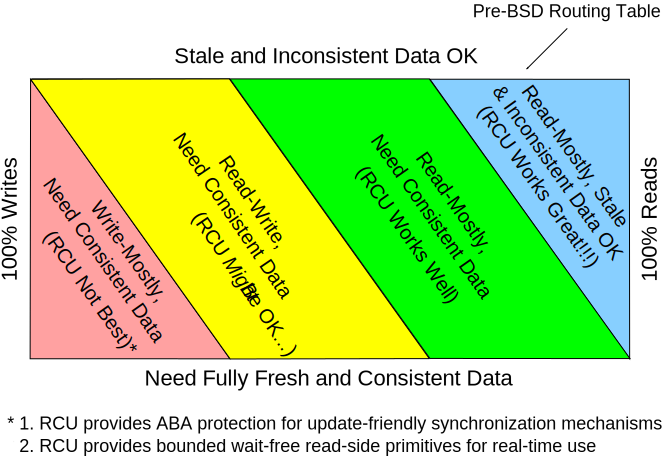
\includegraphics{defer/RCUApplicability}}
\caption{RCU Areas of Applicability}
\label{fig:defer:RCU Areas of Applicability}
\end{figure}

In the meantime,
Figure~\ref{fig:defer:RCU Areas of Applicability}
shows some rough rules of thumb on where RCU is most helpful.

As shown in the blue box at the top of the figure, RCU works best if
you have read-mostly data where stale and inconsistent
data is permissible (but see below for more information on stale and
inconsistent data).
The canonical example of this case in the Linux kernel is routing tables.
Because it may have taken many seconds or even minutes for the
routing updates to propagate across the Internet, the system
has been sending packets the wrong way for quite some time.
Having some small probability of continuing to send some of them the wrong
way for a few more milliseconds is almost never a problem.

If you have a read-mostly workload where consistent data is required,
RCU works well, as shown by the green ``read-mostly, need consistent data''
box.
One example of this case is the Linux kernel's mapping from user-level
System-V semaphore IDs to the corresponding in-kernel data structures.
Semaphores tend to be used far more frequently than they are created
and destroyed, so this mapping is read-mostly.
However, it would be erroneous to perform a semaphore operation on
a semaphore that has already been deleted.
This need for consistency is handled by using the lock in the
in-kernel semaphore data structure, along with a ``deleted''
flag that is set when deleting a semaphore.
If a user ID maps to an in-kernel data structure with the
``deleted'' flag set, the data structure is ignored, so that
the user ID is flagged as invalid.

Although this requires that the readers acquire a lock for the
data structure representing the semaphore itself,
it allows them to dispense with locking for the
mapping data structure.
The readers therefore locklessly
traverse the tree used to map from ID to data structure,
which in turn greatly improves performance, scalability, and
real-time response.

As indicated by the yellow ``read-write'' box, RCU can also be useful
for read-write
workloads where consistent data is required, although usually in
conjunction with a number of other synchronization primitives.
For example, the directory-entry cache in recent Linux kernels uses RCU in
conjunction with sequence locks, per-CPU locks, and per-data-structure
locks to allow lockless traversal of pathnames in the common case.
Although RCU can be very beneficial in this read-write case, such
use is often more complex than that of the read-mostly cases.

Finally, as indicated by the red box at the bottom of the figure,
update-mostly workloads requiring
consistent data are rarely good places to use RCU, though there are some
exceptions~\cite{MathieuDesnoyers2012URCU}.
In addition, as noted in
Section~\ref{sec:defer:RCU Provides Type-Safe Memory},
within the Linux kernel, the \co{SLAB_TYPESAFE_BY_RCU}
slab-allocator flag provides type-safe memory to RCU readers, which can
greatly simplify non-blocking synchronization and other lockless
algorithms.

In short, RCU is an API that includes a publish-subscribe mechanism for
adding new data, a way of waiting for pre-existing RCU readers to finish,
and a discipline of maintaining multiple versions to allow updates to
avoid harming or unduly delaying concurrent RCU readers.
This RCU API is best suited for read-mostly situations, especially if
stale and inconsistent data can be tolerated by the application.

% defer/rcurelated.tex

\subsection{RCU Related Work}
\label{sec:defer:RCU Related Work}
\OriginallyPublished{Section}{sec:defer:RCU Related Work}{RCU Related Work}{Linux Weekly News}{PaulEMcKenney2014ReadMostly}
\OriginallyPublished{Section}{sec:defer:RCU Related Work}{RCU Related Work}{Linux Weekly News}{PaulEMcKenney2015ReadMostly}

RCU 비슷한 것들에 대한 알려진 첫번째 언급은 FORTRAN 을 위한 J. Weizenbaum 의
SLIP 리스트 처리 설비~\cite{Weizenbaum:1963:SLP:367593.367617} 에 대한 Donald
Knuth 의 버그 레포트~\cite[page 413 of Fundamental Algorithms]{Knuth73}
였습니다.
Knuth 는 SLIP 이 grace-period 보장과 같은 것을 갖고 있지 않다고 이야기했습니다.

RCU 비슷한 것들에 대한 버그 레포트가 아닌 첫번째 언급은 Kung 과 Lehman 의
획기적인 논문~\cite{Kung80} 이었습니다.
이 기법의 학계에서의 추가적인
사용~\cite{Manber82,Manber84,BarbaraLiskov1988ArgusCACM,Pugh90,Andrews91textbook,Pu95a,Cowan96a,Rastogi:1997:LPV:645923.671017,Gamsa99}
이 있었습니다만, 이 영역에서의 대부분의 작업은 실제 일을 하는 사람들에 의해
진행되었습니다~\cite{RichardRashid87a,Hennessy89,Jacobson93,AjuJohn95,Slingwine95,Slingwine97,Slingwine98,McKenney98}.
2000 년에 이르러, 주도권은 오픈 소스 프로젝트들로, 그 중에서도 리눅스 커널
커뮤니티로
넘겨졌습니다~\cite{RustyRussell2000a,RustyRussell2000b,McKenney01b,McKenney01a,McKenney02a,Arcangeli03}.\footnote{
	200 개가 넘는 인용처 목록은 이 책의 {\LaTeX} 소스의 \co{bib/RCU.bib}
	에서 찾을 수 있을 겁니다.}
\iffalse

The known first mention of anything resembling RCU took the form of a bug
report from
Donald Knuth~\cite[page 413 of Fundamental Algorithms]{Knuth73}
against J. Weizenbaum's SLIP list-processing facility for
FORTRAN~\cite{Weizenbaum:1963:SLP:367593.367617}.
Knuth was justified in reporting the bug, as SLIP had no notion of
any sort of grace-period guarantee.

The first known non-bug-report mention of anything resembing RCU appeared
in Kung's and Lehman's landmark paper~\cite{Kung80}.
There was some additional use of this technique in
academia~\cite{Manber82,Manber84,BarbaraLiskov1988ArgusCACM,Pugh90,Andrews91textbook,Pu95a,Cowan96a,Rastogi:1997:LPV:645923.671017,Gamsa99},
but much of the work in this area was carried out by
practitioners~\cite{RichardRashid87a,Hennessy89,Jacobson93,AjuJohn95,Slingwine95,Slingwine97,Slingwine98,McKenney98}.
By the year 2000, the initiative had passed to open-source projects,
most notably the Linux kernel
community~\cite{RustyRussell2000a,RustyRussell2000b,McKenney01b,McKenney01a,McKenney02a,Arcangeli03}.\footnote{
	A list of citations with well over 200 entries may be found in
	\co{bib/RCU.bib} in the {\LaTeX} source for this book.}
\fi

하지만, 2010년대 중반에 이르러, 커뮤니티와 기관들을 통한 RCU 에 대한 연구와
개발~\cite{FransKaashoek2015ParallelOSHistory} 이 급증했습니다.
Section~\ref{sec:defer:RCU Uses} 는 RCU 의 사용들에 대해 설명하고,
Section~\ref{sec:defer:RCU Implementations} 는 RCU 구현들을 (그리고 구현을
반들고 사용한 일들도) 설명하고, 마지막으로,
Section~\ref{sec:defer:RCU Validation} 에서는 RCU 의 검증과 그 사용을
이야기합니다.
\iffalse

However, in the mid 2010s, there was a welcome upsurge in RCU research
and development across a number of communities and
institutions~\cite{FransKaashoek2015ParallelOSHistory}.
Section~\ref{sec:defer:RCU Uses} describes uses of RCU,
Section~\ref{sec:defer:RCU Implementations} describes RCU implementations
(as well as work that both creates and uses an implementation),
and finally,
Section~\ref{sec:defer:RCU Validation} describes verification and validation
of RCU and its uses.
\fi

\subsubsection{RCU Uses}
\label{sec:defer:RCU Uses}

Portland State University (PSU) 의 Phil Howard 와 Jon Walpole 은 RCU 를
소프트웨어 트랜잭셔널 메모리를 사용해 동기화된 업데이트와 조합해서 red-black
tree 에 적용~\cite{PhilHowardPhD,PhilHoward2011RCUTMRBTree} 했습니다.
Josh Priplett 과 Jon Walpole (다시 말하지만 PSU) 은 RCU 를 resizable hash table
에
적용했습니다~\cite{JoshTriplettPhD,Triplett:2011:RPHash,JonCorbet2014RCUhash1,JonCorbet2014RCUhash2}.
RCU 로 보호되는 또다른 resizable hash table 이 Herbert
Xu~\cite{HerbertXu2010RCUResizeHash} 와 Mathieu
Desnoyers~\cite{PaulMcKenney2013LWNURCUhash} 에 의해 만들어졌습니다.
\iffalse

Phil Howard and Jon Walpole of Portland State University (PSU) have
applied RCU to red-black
trees~\cite{PhilHowardPhD,PhilHoward2011RCUTMRBTree} combined with updates
synchronized using software transactional memory.
Josh Triplett and Jon Walpole (again of PSU) applied RCU to resizable
hash tables~\cite{JoshTriplettPhD,Triplett:2011:RPHash,JonCorbet2014RCUhash1,JonCorbet2014RCUhash2}.
Other RCU-protected resizable hash tables have been created by
Herbert Xu~\cite{HerbertXu2010RCUResizeHash} and by
Mathieu Desnoyers~\cite{PaulMcKenney2013LWNURCUhash}.
\fi

MIT 의 Austin Clements, Frans Kaashoek, 그리고 Nickolai Zeldovich 는 RCU 에
최적화된 balanced binary tree (Bosai)~\cite{AustinClements2012RCULinux:mmapsem}
을 만들었고, 리눅스 커널의 \co{mmap_sem} 의 read-side contention 을 줄이기 위해
이 트리를 리눅스 커널의 VM 에 적용했습니다.
이 작업은 많은 수의 minor page fault 로 구성된 microbenchmark 에서 최소 80 개의
CPU 들까지는 열배 이상의 속도 향상과 확장성을 보였습니다.
이는 앞서 Pter Zijlstra 에 의해 개발된
패치~\cite{PeterZijlstra2014SpeculativePageFault} 와 비슷하며, 둘 다 파일시스템
데이터 구조는 RCU 읽기 쓰레드들에게 안전하지 않다는 한계점을 가지고 있습니다.
Clements 등은 이 한계점을 page-fault 처리 경로를 anonymous page 들로만
제한함으로써 피했습니다.
더 최근에 들어서는 파일시스템 데이터 구조도 RCU 읽기 쓰레드들에게 안전하게
되었고~\cite{JonathanCorbet2010dcacheRCU,JonathanCorbet2011dcacheRCUbug},
따라서 이 작업은 anonymous page 만이 아니라 모든 종류의 page 들에 대해 구현될
수 있을 겁니다---실제로, Peter Zijlstra 는 최근에 이에 대한 프로토타입을
만들었습니다.
\iffalse

Austin Clements, Frans Kaashoek, and Nickolai Zeldovich
of MIT created an RCU-optimized balanced binary tree
(Bonsai)~\cite{AustinClements2012RCULinux:mmapsem}, and applied this
tree to the Linux kernel's VM subsystem in order to reduce read-side
contention on the Linux kernel's \co{mmap_sem}.
This work resulted in order-of-magnitude speedups and scalability up to
at least 80 CPUs for a microbenchmark featuring large numbers of minor
page faults.
This is similar to a patch developed earlier by
Peter Zijlstra~\cite{PeterZijlstra2014SpeculativePageFault}, and both
were limited by the fact that, at the time, filesystem data structures
were not safe for RCU readers.
Clements et al. avoided this limitation by optimizing the page-fault
path for anonymous pages only.
More recently, filesystem data structures have been made safe for RCU
readers~\cite{JonathanCorbet2010dcacheRCU,JonathanCorbet2011dcacheRCUbug},
so perhaps this work can be implemented for all page types, not just
anonymous pages---Peter Zijlstra has, in fact, recently prototyped
exactly this.
\fi

MIT 의 Yandong Mao 와 Robert Morris, 그리고 Harvard University 의 Eddie Kohler
는 B+ tree 와 tries 의 아이디어를 조합한, Masstree 라는 이름의, RCU 로 보호되는
또다른 트리를 만들었습니다~\cite{Mao:2012:CCF:2168836.2168855}.
이 tree 는 RCU 로 보호되는 hash table 에 비해 2.5배 가량 느리지만 hash table 과
달리 key range 에 대한 오퍼레이션들을 지원합니다.
또한, Masstree 는 긴 shared key prefix 에 대해 효율적인 오브젝트 저장소를
지원하며, 더 나아가서 대용량 저장소로의 로깅을 통한 persistency 를 제공합니다.

해당 페이퍼는 Masstree 의 성능이 memcached 의 것과 견주어질 수 있으며, 심지어
Masstree 는 memcached 가 제공하지 않는 업데이트의 지속성을 제공한다고 이야기
했습니다.
이 논문은 또한 Masstree 의 성능을 지속성 있는 데이터베이스인 MongoDB, VoltDB,
Redis 와 비교해서 어떤 경우에는 100배가 넘는 성능 이득을 보였습니다.
MIT 의 Stephen Tu, Wenting Zheng, Barbara Liskov, 그리고 Samuel Madden 과
Kohler 의 또다른 논문~\cite{Tu:2013:STM:2517349.2522713} 은 Masstree 를 Silo
라는 이름의 in-memory 데이터베이스에 적용해서 잘 알려진 트랜잭션 처리
벤치마크에서 초당 700K 트랜잭션 (분당 42M 트랜잭션) 을 달성했습니다.
흥미롭게도, Silo 는 락을 잡으면서 grace period 의 오버헤드를 일으키지 않고도
linearizability 를 보장합니다.
\iffalse

Yandong Mao and Robert Morris of MIT and Eddie Kohler of
Harvard University created another RCU-protected tree named
Masstree~\cite{Mao:2012:CCF:2168836.2168855} that combines ideas from B+
trees and tries.
Although this tree is about 2.5x slower than an RCU-protected hash table,
it supports operations on key ranges, unlike hash tables.
In addition, Masstree supports efficient storage of objects with long
shared key prefixes and, furthermore, provides persistence via logging
to mass storage.

The paper notes that Masstree's performance rivals that of memcached, even
given that Masstree is persistently storing updates and memcached is not.
The paper also compares Masstree's performance to the persistent
datastores MongoDB, VoltDB, and Redis, reporting significant performance
advantages for Masstree, in some cases exceeding two orders of magnitude.
Another paper~\cite{Tu:2013:STM:2517349.2522713}, by Stephen Tu,
Wenting Zheng, Barbara Liskov, and Samuel Madden of MIT and Kohler,
applies Masstree to an in-memory database named Silo, achieving 700K
transactions per second (42M transactions per minute) on a well-known
transaction-processing benchmark.
Interestingly enough, Silo guarantees linearizability without incurring
the overhead of grace periods while holding locks.
\fi

Technion 의 Maya Arbel 과 Hagit Attiya 는 Masstree 와 같이 동시의 업데이트를
가능하게 해주는 더 정밀한 방법~\cite{MayaArbel2014RCUtree} 을 RCU 로 보호되는
탐색 tree 에 적용했습니다.
이 논문은 올바름의 증명과 이 tree 의 모든 오퍼레이션들이 linearizable 하다는
증명을 포함합니다.
불행히도, 이 구현은 lock 을 잡으면서 기다리는 동안 grace-period 전체 응답시간을
필요로 함으로써 linearizability 를 얻는데, 이는 update 로만 이루어진 workload
에서는 확장성을 떨어뜨립니다.
이 문제를 해결하는 한가지 방법은 linearizability 를 포기하는
것~\cite{AndreasHaas2012FIFOisnt,PaulEMcKennneyAtomicTreeN4037} 입니다만, Arbel
과 Attiya 는 그대신 low-end grace-period 응답시간을 줄인 RCU 변종을
만들었습니다.
물론, 어떤 것도 공짜로 얻어지지는 않고, 이 RCU 변종은 32개 CPU 에서 확장성의
한계를 드러내는 결과를 나타냈습니다.
Linearizability 를 포기해서 성능과 확장성을 모두 얻는 것에 대해서도 더 이야기
할 부분이 많지만, 학계에서 대안적 RCU 구현들로 한 실험들을 보는 것도 좋을
겁니다.
\iffalse

Maya Arbel and Hagit Attiya of Technion took a more rigorous
approach~\cite{MayaArbel2014RCUtree} to an RCU-protected search tree that,
like Masstree, allows concurrent updates.
This paper includes a proof of correctness, including proof that all
operations on this tree are linearizable.
Unfortunately, this implementation achieves linearizability by incurring
the full latency of grace-period waits while holding locks, which degrades
scalability of update-only workloads.
One way around this problem is to abandon
linearizability~\cite{AndreasHaas2012FIFOisnt,PaulEMcKennneyAtomicTreeN4037}),
however, Arbel and Attiya instead created an RCU variant that reduces
low-end grace-period latency.
Of course, nothing comes for free, and this RCU variant appears to hit
a scalability limit at about 32 CPUs.
Although there is much to be said for dropping linearizability, thus
gaining both performance and scalability, it is very good to see academics
experimenting with alternative RCU implementations.
\fi

\subsubsection{RCU Implementations}
\label{sec:defer:RCU Implementations}

Mathieu Desnoyers 는 tracing 에 사용하기 위해 user-space RCU 를
만들었고~\cite{MathieuDesnoyers2009URCU,MathieuDesnoyersPhD,MathieuDesnoyers2012URCU}
이는 여러 프로젝트들~\cite{MikeDay2013RCUqemu} 에 사용되었습니다.

프라하에 위치한 Charles University 의 연구원들 역시 RCU 구현들에 대한 연구를
진행했는데, Andrej Podzimek 의 박사 학위 논문~\cite{AndreasHaas2012FIFOisnt} 과
Adam Hraska 의 박사학위 논문~\cite{AdamHraska2013RCUHelenOS} 이 그것들입니다.

Yujie Liu (Lehigh University), Victor Luchangco (Oracle Labs), 그리고
Michael Spear (Lehigh University)~\cite{Liu:2013:MSA:2549695.2549732} 는
서비스에 scalable non-zero indicators (SNZI)~\cite{FaithEllen:2007:SNZI} 를
사용했습니다.
여기서 의도된 목적은 결국은 확장성을 제한할 수 있는, linearizability 를 갖는
software transactional memory
(Section~\ref{sec:future:Transactional Memory} 를 참고하세요) 를 구현하는
것입니다.
\iffalse

Mathieu Desnoyers created a user-space RCU for use in
tracing~\cite{MathieuDesnoyers2009URCU,MathieuDesnoyersPhD,MathieuDesnoyers2012URCU},
which has seen use in a number of projects~\cite{MikeDay2013RCUqemu}.

Researchers at Charles University in Prague have also been
working on RCU implementations, including dissertations by
Andrej Podzimek~\cite{AndrejPodzimek2010masters} and Adam
Hraska~\cite{AdamHraska2013RCUHelenOS}.

Yujie Liu (Lehigh University), Victor Luchangco (Oracle Labs), and
Michael Spear (also Lehigh)~\cite{Liu:2013:MSA:2549695.2549732}
pressed scalable non-zero indicators
(SNZI)~\cite{FaithEllen:2007:SNZI} into service as a grace-period
mechanism.
The intended use is to implement software transactional memory
(see Section~\ref{sec:future:Transactional Memory}), which
imposes linearizability requirements, which in turn seems to
limit scalability.
\fi

RCU 같은 메커니즘들이 Java 에도 도입되고 있습니다.
Sivaramakrishnan 등~\cite{Sivaramakrishnan:2012:ERB:2258996.2259005} 은 RCU
같은 메커니즘을 사용해서 Java 의 가비지 콜렉터와 상호작용할 때 필요한 read
barrier 를 제거해 상당한 성능 향상을 냈습니다.

Shanghai Jiao Tong University 의 Ran Liu, Heng Zhang, 그리고 Haibo Chen 은
최적화된 ``passive reader-writer lock'' 에 사용하기 위한 특수화된 RCU
변종~\cite{RanLiu2014PassiveRWLock} 을 만들었는데, 이는 Gautham
Shenoy~\cite{GauthamShenoy2006RCUrwlock} 의 것과 Srivatsa
Bhat~\cite{SrivatsaSBhat2014RCUrwlock} 의 것과 비슷합니다.
Liu 등의 논문은 여러 측면에서 흥미롭습니다~\cite{PaulEMcKenney2014ReadMostly}.
\iffalse

RCU-like mechanisms are also finding their way into Java.
Sivaramakrishnan et al.~\cite{Sivaramakrishnan:2012:ERB:2258996.2259005}
use an RCU-like mechanism to eliminate the read barriers that are
otherwise required when interacting with Java's garbage collector,
resulting in significant performance improvements.

Ran Liu, Heng Zhang, and Haibo Chen of Shanghai Jiao Tong University
created a specialized variant of RCU that they used for an optimized
``passive reader-writer lock''~\cite{RanLiu2014PassiveRWLock}, similar to
those created by Gautham Shenoy~\cite{GauthamShenoy2006RCUrwlock} and
Srivatsa Bhat~\cite{SrivatsaSBhat2014RCUrwlock}.
The Liu et al.~paper is interesting from a number of
perspectives~\cite{PaulEMcKenney2014ReadMostly}.
\fi

Mike Ash 는 Apple 의 Objective-C 런타임에 있는 RCU 같은 기능들에 대한 설명을
기재했습니다~\cite{MikeAsh2015Apple}.
이 방법은 read-side 크리티컬 섹션들을 코드 영역을 이야기하는 것으로 파악하게
하고, 이로 인해 다른 제로에 가까운 read-side 오버헤드를 달성하는 방법들처럼
높은 성능을 보입니다만, 여러 함수들로 구성되는 커다란 read-side 크리티컬
섹션들을 어떻게 다룰 것인지에 대한 실용적인 측면의 도전사항을 갖습니다.

Pedro Ramalhete 와 Andreia Correia~\cite{PedroRmalhete2015PoorMansRCU} 는
``Poor Man's RCU'' 를 만들었는데, 이는 reader-writer 락 한쌍을 사용하면서도
읽기 쓰레드들에게 lock-free forward-progress guarantee 를
제공합니다~\cite{PaulEMcKenney2015ReadMostly}.

Maya Arble 과 Adam Morrison~\cite{Arbel:2015:PRR:2858788.2688518} 은
``Predicate RCU'' 를 만들었는데, 이는 update-side 락들을 grace period 들 사이로
갖는 알고리즘들을 효과적으로 지원하기 위해 grace-period 기간을 줄이려
노력합니다.
이는 grace period 들 사이로의 업데이트의 batching 을 줄이고 확장성을 줄이는
결과를 초래했습니다만, 짧은 grace period 를 제공하는 데에는 성공했습니다.
\iffalse

Mike Ash posted~\cite{MikeAsh2015Apple} a description of an RCU-like
primitive in Apple's Objective-C runtime.
This approach identifies read-side critical sections via designated
code ranges, thus qualifying as another method of achieving
zero read-side overhead, albeit one that poses some interesting
practical challenges for large read-side critical sections that
span multiple functions.

Pedro Ramalhete and Andreia Correia~\cite{PedroRmalhete2015PoorMansRCU}
produced ``Poor Man's RCU'', which, despite using a pair of reader-writer
locks, manages to provide lock-free forward-progress guarantees to
readers~\cite{PaulEMcKenney2015ReadMostly}.

Maya Arbel and Adam Morrison~\cite{Arbel:2015:PRR:2858788.2688518}
produced ``Predicate RCU'', which works hard to reduce grace-period
duration in order to efficiently support algorithms that hold
update-side locks across grace periods.
This results in reduced batching of updates into grace periods
and reduced scalability, but does succeed in providing short
grace periods.
\fi

\QuickQuiz{}
	Grace period 를 기다리기 전에 락을 내려놓거나 grace period 를 기다리는
	대신에 \co{call_rcu()} 같은 걸 사용하는 게 어떤가요?
	\iffalse

	Why not just drop the lock before waiting for the grace
	period, or using something like \co{call_rcu()}
	instead of waiting for a grace period?
	\fi
\QuickQuizAnswer{
	이 저자들은 linearizable tree 오퍼레이션들을 지원하고자 했고, 따라서
	동시의 트리에 대한 추가, 삭제, 그리고 탐색은 전체적으로 동의된 순서로
	수행된 것으로 나타나야 했습니다.
	이들의 탐색 트리에서는, 이 grace period 들 사이로 락을 잡을 것을 필요로
	했습니다.
	(대부분의 경우에는 linearizability 를 버리는게 낫겠습니다만,
	linearizabiliy 는 놀랍도록 대중적인 (그리고 비싼!) 요구사항입니다.)
	\iffalse

	The authors wished to support linearizable tree
	operations, so that concurrent additions to, deletions
	from, and searches of the tree would appear to execute
	in some globally agreed-upon order.
	In their search trees, this requires holding locks
	across grace periods.
	(It is probably better to drop linearizability as a
	requirement in most cases, but linearizability is a
	surprisingly popular (and costly!) requirement.)
	\fi
} \QuickQuizEnd

Alexander Matveev (MIT), Nir Shavit (MIT and Tel-Aviv University),
Pascal Felber (University of Neuch\^{a}tel), 그리고 Patrick Marlier (also
University of Neuch\^{a}tel)~\cite{Matveev:2015:RLS:2815400.2815406}
은 명시적으로 read-only 트랜잭션들을 표시하는 software transactional memory
라고 생각될 수 있는 RCU 같은 메커니즘을 만들었습니다.
이들의 사용예는 grace period 들 사이로 락을 잡을 것을 필요로 하는데, 이는
확장성을
제한합니다~\cite{PaulEMcKenney2015ReadMostly,PaulEMcKenney2015ReadMostlySidebar}.
이는 \co{rcutorture} 테스트 도구를 잘 사용한 첫번째 학계의 RCU 관련
작업이었으며, 성능 향상 내용을 Linux-kernel RCU 에 제출한 첫번째였는데, v4.4 에
받아들여졌습니다.

Geoff Romer 와 Andrew Hunter (둘 다 Google) 는 싱글톤 데이터 구조체의 RCU
보호를 위한 cell 기반 API 를 C++ 표준에 포함될 수 있도록
제안했습니다~\cite{GeoffRomer2017C++DeferredReclamation}.
\iffalse

Alexander Matveev (MIT), Nir Shavit (MIT and Tel-Aviv University),
Pascal Felber (University of Neuch\^{a}tel), and Patrick Marlier (also
University of Neuch\^{a}tel)~\cite{Matveev:2015:RLS:2815400.2815406}
produced an RCU-like mechanism that can be thought of as
software transactional memory that explicitly marks
read-only transactions.
Their use cases require holding locks across grace periods, which limits
scalability~\cite{PaulEMcKenney2015ReadMostly,PaulEMcKenney2015ReadMostlySidebar}.
This appears to be the first academic RCU-related work to
make good use of the \co{rcutorture} test suite, and also the
first to have submitted a performance improvement to Linux-kernel
RCU, which was accepted into v4.4.

Geoff Romer and Andrew Hunter (both at Google) proposed a cell-based API for RCU
protection of singleton data structures for inclusion in the
C++ standard~\cite{GeoffRomer2017C++DeferredReclamation}.
\fi

\subsubsection{RCU Validation}
\label{sec:defer:RCU Validation}

2017 년 초에 이르러 모든 버그가 잠재적 보안 취약점이라는 것이 일반적으로
알려졌고, 따라서 검증은 첫번째로 신경써야 할 영역입니다.

Stony Brook University 의 연구자들은 RCU 를 인지하는 data-race
detector~\cite{AbhinavDuggal2010Masters,JustinSeyster2012PhD,Seyster:2011:RFA:2075416.2075425}
를 만들었습니다.
IMDEA 의 Alexey Gotsman, Tel Aviv University 의 Noam Rinetzky, 그리고
University of Oxford 의 Hongseok Yang 은 RCU 의 형식적 semantic 들을 speration
logic 의 용어로 표현하는 논문~\cite{AlexeyGotsman2012VerifyGraceExtended} 을
발표했고 동시성의 다른 영역에 대해서도 작업을 계속하고 있습니다.
\iffalse

In early 2017, it is commonly recognized that almost any bug is a potential
security exploit, so validation and verification are first-class concerns.

Researchers at Stony Brook University have produced an RCU-aware data-race
detector~\cite{AbhinavDuggal2010Masters,JustinSeyster2012PhD,Seyster:2011:RFA:2075416.2075425}.
Alexey Gotsman of IMDEA, Noam Rinetzky of Tel Aviv University,
and Hongseok Yang of the University of Oxford have published a
paper~\cite{AlexeyGotsman2012VerifyGraceExtended} expressing the formal
semantics of RCU in terms of separation logic, and have continued with
other aspects of concurrency.
\fi

Joseph Tassarotti (Carnegie-Mellon University), Derek Dreyer (Max
Planck Institute for Software Systems), 그리고 Viktor Vafeiadis
(MPI-SWS)~\cite{JosephTassarotti2015RCUproof} 는 userspace RCU 의
quiescent-state-based-reclamation (QSBR) 변종의 올바름에 대한 manual formal
proof 를 만들었습니다.
Lihao Liang (University of Oxford), Paul E.~McKenney (IBM),
Daniel Kroening, 그리고 Tom Melham
(둘 다 Oxford)~\cite{LihaoLiang2016VerifyTreeRCU} 는 C bounded model checker
(CBMC)~\cite{EdmundClarke2004CBMC} 를 사용해 Linux-kernel Tree RCU 의 상당한
부분에 대한 올바름의 기계적 증명을 만들어냈습니다.
Lance Roy~\cite{LanceRoy2017CBMC-SRCU} 는 CBMC 를 사용해서 Linux-kernel
sleepable RCU (SRCU)~\cite{PaulEMcKenney2006c} 의 상당한 부분에 대한 올바름의
증명을 만들었습니다.
마지막으로, Michalis Kokologiannakis 와 Konstantinos Sagonas (National
Technical University of Athens)~\cite{MichalisKokologiannakis2017NidhuggRCU}
는 Nighugg tool~\cite{CarlLeonardsson2014Nidhugg} 을 사용해서 Linux-kernel Tree
RCU 의 더 커다란 영역에 대해 기계적 올바름의 증명을 만들어냈습니다.
\iffalse

Joseph Tassarotti (Carnegie-Mellon University), Derek Dreyer (Max
Planck Institute for Software Systems), and Viktor Vafeiadis
(also MPI-SWS)~\cite{JosephTassarotti2015RCUproof}
produced a manual formal proof of correctness of the quiescent-state-based
reclamation (QSBR) variant of userspace
RCU~\cite{MathieuDesnoyers2009URCU,MathieuDesnoyers2012URCU}.
Lihao Liang (University of Oxford), Paul E.~McKenney (IBM),
Daniel Kroening, and Tom Melham
(both also Oxford)~\cite{LihaoLiang2016VerifyTreeRCU}
used the C bounded model checker (CBMC)~\cite{EdmundClarke2004CBMC}
to produce a mechanical proof of correctness of a significant portion
of Linux-kernel Tree RCU.
Lance Roy~\cite{LanceRoy2017CBMC-SRCU} used CBMC to produce a similar
proof of correctness for a significant portion of Linux-kernel
sleepable RCU (SRCU)~\cite{PaulEMcKenney2006c}.
Finally, Michalis Kokologiannakis and Konstantinos Sagonas (National Technical University of
Athens)~\cite{MichalisKokologiannakis2017NidhuggRCU}
used the Nighugg tool~\cite{CarlLeonardsson2014Nidhugg}
to produce a mechanical proof of correctness of a somewhat larger
portion of Linux-kernel Tree RCU.
\fi

이러한 노력들 중 어느 것도 해당 검증 도구들을 테스트하는데에 관여된 RCU 버그들
외에는 어떤 버그도 찾아내지 않았습니다.
반대로,
Alex Groce (Oregon State University), Iftekhar Ahmed, Carlos Jensen
(둘 다 OSU), 그리고 Paul E.~McKenney
(IBM)~\cite{Groce:2015:VMC:2916135.2916190}
는 \co{rcutorture} 테스트 도구의 적용 범위를 테스트 하기 위해 리눅스 커널 RCU
의 소스 코드를 자동적으로 변형시켰습니다.
이 방법은 이 테스트 도구의 적용 범위에 있는 여러 구멍들을 찾아냈으며, 그 중
하나는 Tiny RCU 의 진짜 버그 (지금은 고쳐진) 가 숨겨져 있는 것을 찾아냈습니다.

운이 좋다면, 이런 검증에 대한 작업들은 모두 결국은 동시성 코드의 검증을 위한 더
나은 도구들을 생겨나게 할겁니다.
\iffalse

None of these efforts located any bugs other than bugs injected into
RCU specifically to test the verification tools.
In contrast,
Alex Groce (Oregon State University), Iftekhar Ahmed, Carlos Jensen
(both also OSU), and Paul E.~McKenney
(IBM)~\cite{Groce:2015:VMC:2916135.2916190}
automatically mutated Linux-kernel RCU's source code to test the
coverage of the \co{rcutorture} test suite.
The effort found several holes in this suite's coverage, one of which
was hiding a real bug (since fixed) in Tiny RCU.

With some luck, all of this validation work will eventually result in
more and better tools for validating concurrent code.
\fi


% defer/rcuexercises.tex
% SPDX-License-Identifier: CC-BY-SA-3.0

\subsection{RCU Exercises}
\label{sec:defer:RCU Exercises}

이 섹션은 RCU 를 이 책에서 앞서 보인 여러 예제들에 적용하는 내용에 대한
여러개의 Quick Quizz 들로 구성되어 있습니다.
각 Quick Quiz 에의 답은 힌트를 일부 제공하고, 또한 그 해법이 자세히 설명되어
있는 뒤의 섹션으로의 포인터를 담고 있습니다.
\co{rcu_read_lock()}, \co{rcu_read_unlock()}, \co{rcu_dereference()},
\co{rcu_assign_pointer()}, 그리고 \co{synchronize_rcu()} 기능들만으로도 이
문제들에 충분해야 할 겁니다.
\iffalse

This section is organized as a series of Quick Quizzes that invite you
to apply RCU to a number of examples earlier in this book.
The answer to each Quick Quiz gives some hints, and also contains a
pointer to a later section where the solution is explained at length.
The \co{rcu_read_lock()}, \co{rcu_read_unlock()}, \co{rcu_dereference()},
\co{rcu_assign_pointer()}, and \co{synchronize_rcu()} primitives should
suffice for most of these exercises.
\fi

\QuickQuiz{}
	Figure~\ref{fig:count:Per-Thread Statistical Counters}
	(\path{count_end.c})
	에 보인 통계적 카운터의 구현은 \co{read_count()} 안에서 합계를 구하는
	것을 보호하기 위해 글로벌 락을 사용했는데 이는 부족한 성능과 음의
	확장성을 일으켰습니다.
	\co{read_count()} 가 훌륭한 성능과 좋은 확장성을 제공할 수 있게 하기
	위해 RCU 를 어떻게 적용해 볼 수 있을까요.
	(\co{read_count()} 의 확장성은 모든 쓰레드의 카운터들을 스캔해야 한다는
	필요성으로 인해 제한되어진다는 점을 명심하세요.)
	\iffalse

	The statistical-counter implementation shown in
	Listing~\ref{lst:count:Per-Thread Statistical Counters}
	(\path{count_end.c})
	used a global lock to guard the summation in \co{read_count()},
	which resulted in poor performance and negative scalability.
	How could you use RCU to provide \co{read_count()} with
	excellent performance and good scalability.
	(Keep in mind that \co{read_count()}'s scalability will
	necessarily be limited by its need to scan all threads'
	counters.)
	\fi
\QuickQuizAnswer{
	힌트: 글로벌 변수 \co{finalcount} 와 배열 \co{counterp[]} 를 하나의 RCU
	로 보호되는 구조체 안에 넣으세요.
	초기화 때, 이 구조체는 할당되고 모두 0과 \co{NULL} 로 설정될 겁니다.

	\co{inc_count()} 함수는 바뀔 필요가 없을 겁니다.

	\co{read_count()} 함수는 \co{final_mutex} 를 잡는 대신에
	\co{rcu_read_lock()} 를 사용할 것이고, 현재 구조체로의 레퍼런스를
	얻어오는데에 \co{rcu_dereference()} 를 사용해야 할겁니다.
	\iffalse

	Hint: place the global variable \co{finalcount} and the
	array \co{counterp[]} into a single RCU-protected struct.
	At initialization time, this structure would be allocated
	and set to all zero and \co{NULL}.

	The \co{inc_count()} function would be unchanged.

	The \co{read_count()} function would use \co{rcu_read_lock()}
	instead of acquiring \co{final_mutex}, and would need to
	use \co{rcu_dereference()} to acquire a reference to the
	current structure.
	\fi

	\co{count_register_thread()} 함수는 이 새로 생성된 쓰레드와 연관된 배열
	원소를 그 쓰레드의 쓰레드별 \co{counter} 변수로의 레퍼런스로 설정할
	겁니다.

	\co{count_unregister_thread()} 함수는 새로운 구조체를 할당받고,
	\co{final_mutex} 를 잡은 후, 기존의 구조체를 새로운 것으로 복사하고,
	나가는 쓰레드의 \co{counter} 변수를 전체 값에 더하고, 이 \co{counter}
	변수로의 포인터를 \co{NULL} 로 만든 후, 이 새로운 구조체를 과거의 것의
	자리에 설치하기 위해 \co{rcu_assign_pointer()} 를 사용한 후,
	\co{final_mutex} 를 풀고, grace period 를 기다린 후, 마지막으로 기존의
	구조체를 메모리 해제시켜야 할 것입니다.
	\iffalse

	The \co{count_register_thread()} function would set the
	array element corresponding to the newly created thread
	to reference that thread's per-thread \co{counter} variable.

	The \co{count_unregister_thread()} function would need to
	allocate a new structure, acquire \co{final_mutex},
	copy the old structure to the new one, add the outgoing
	thread's \co{counter} variable to the total, \co{NULL}
	the pointer to this same \co{counter} variable,
	use \co{rcu_assign_pointer()} to install the new structure
	in place of the old one, release \co{final_mutex},
	wait for a grace period, and finally free the old structure.
	\fi

	이게 정말 동작할까요?
	그 이유는 무엇이죠?

	더 자세한 내용을 위해서는
	page~\pageref{sec:together:RCU and Per-Thread-Variable-Based Statistical Counters}
	의
	Section~\ref{sec:together:RCU and Per-Thread-Variable-Based Statistical Counters}
	를 참고하세요.
	\iffalse

	Does this really work?
	Why or why not?

	See
	Section~\ref{sec:together:RCU and Per-Thread-Variable-Based Statistical Counters}
	on
	page~\pageref{sec:together:RCU and Per-Thread-Variable-Based Statistical Counters}
	for more details.
	\fi
} \QuickQuizEnd


\QuickQuiz{}
	Section~\ref{sec:count:Applying Specialized Parallel Counters}
	는 디바이스들을 제거하기 위해 I/O 액세스들을 카운트하는 일을 처리하는
	한쌍의 코드 조각들을 보였습니다.
	이 코드 조각들은 reader-writer 락을 잡아야 하는 이유로 (I/O 를
	시작하는) 빠른 수행 경로의 높은 오버헤드 문제를 겪었습니다.
	여기에 훌륭한 성능과 확장성을 가져오기 위해 RCU 를 어떻게 사용할 수
	있을까요?
	(I/O 액세스를 하는 일반적인 경우의 첫번째 코드 조각의 성능이 디바이스
	제거 코드 조각의 것보다 훨씬 더 중요함을 명심하세요.)
	\iffalse

	Section~\ref{sec:count:Applying Specialized Parallel Counters}
	showed a fanciful pair of code fragments that dealt with counting
	I/O accesses to removable devices.
	These code fragments suffered from high overhead on the fastpath
	(starting an I/O) due to the need to acquire a reader-writer
	lock.
	How would you use RCU to provide excellent performance and
	scalability?
	(Keep in mind that the performance of the common-case first
	code fragment that does I/O accesses is much more important
	than that of the device-removal code fragment.)
	\fi
\QuickQuizAnswer{
	힌트: 이 reader-writer 락의 read 권한 획득을 RCU read-side 크리티컬
	섹션들로 바꾸고, device 제거 코드를 이에 맞게 조정하세요.
	이 문제에 대한 하나의 해결책을 위해선
	Page~\pageref{sec:together:RCU and Counters for Removable I/O Devices}
	의
	Section~\ref{sec:together:RCU and Counters for Removable I/O Devices}
	를 참고하세요.
	\iffalse

	Hint: replace the read-acquisitions of the reader-writer lock
	with RCU read-side critical sections, then adjust the
	device-removal code fragment to suit.

	See
	Section~\ref{sec:together:RCU and Counters for Removable I/O Devices}
	on
	Page~\pageref{sec:together:RCU and Counters for Removable I/O Devices}
	for one solution to this problem.
	\fi
} \QuickQuizEnd

% defer/whichtochoose.tex
% SPDX-License-Identifier: CC-BY-SA-3.0

\section{Which to Choose?}
\label{sec:defer:Which to Choose?}

\begin{table*}
\small
\centering
\begin{tabular}{p{1.5in}||p{1.5in}|p{0.8in}|p{0.8in}|p{1.0in}}
	~ ~ ~ ~ ~ ~ ~ ~ ~
		& Reference Counting
			& Hazard Pointers
				& Sequence Locks
					& RCU \\
	\hline
%		  RC	  HP	  SL	  RCU \\
	\hline
	Existence Guarantees
		& Complex
			& Yes
				& No
					& Yes \\
	\hline
	Updates and Readers Progress Concurrently
		& Yes
			& Yes
				& No
					& Yes \\
	\hline
	Contention Among Readers
		& High
			& None
				& None
					& None \\
	\hline
	Reader Per-Critical-Section Overhead
		& N/A
			& N/A
				& Two \co{smp_mb()}
					& Ranges from none to two
					  \co{smp_mb()} \\
	\hline
	Reader Per-Object Traversal Overhead
		& Read-modify-write atomic operations, memory-barrier
		  instructions, and cache misses
			& \co{smp_mb()}
				& None, but unsafe
					& None (volatile accesses) \\
	\hline
	Reader Forward Progress Guarantee
		& Lock free
			& Lock free
				& Blocking
					& Bounded wait free \\
	\hline
	Reader Reference Acquisition
		& Can fail (conditional)
			& Can fail (conditional)
				& Unsafe
					& Cannot fail (unconditional) \\
	\hline
	Memory Footprint
		& Bounded
			& Bounded
				& Bounded
					& Unbounded \\
	\hline
	Reclamation Forward Progress
		& Lock free
			& Lock free
				& N/A
					& Blocking \\
	\hline
	Automatic Reclamation
		& Yes
			& No
				& N/A
					& No \\
	\hline
	Lines of Code
		& 94
			& 79
				& 79
					& 73 \\
\end{tabular}
\caption{Which Deferred Technique to Choose?}
\label{tab:defer:Which Deferred Technique to Choose?}
\end{table*}

Table~\ref{tab:defer:Which Deferred Technique to Choose?}
는 이 챕터에서 소개한 네개의 미뤄두고 처리하기 테크닉들 중 무엇을
선택해야할지를 돕는 대략적 경험적 법칙을 제공합니다.

``Existence Guarantee'' 행에서 보인 것처럼, 링크된 데이터 원소들에 대한 존재
보장이 필요하다면 레퍼런스 카운팅, 해저드 포인터, 또는 RCU 를 사용해야 합니다.
시퀀스 락은 존재 보장을 제공하지 않고, 업데이트의 발견과 업데이트를 마주한
read-side 크리티컬 섹션의 재시도 기능을 제공합니다.
\iffalse

Table~\ref{tab:defer:Which Deferred Technique to Choose?}
provides some rough rules of thumb that can help you choose among the
four deferred-processing techniques presented in this chapter.

As shown in the ``Existence Guarantee'' row,
if you need existence guarantees for linked
data elements, you must use reference counting, hazard pointers, or RCU.
Sequence locks do not provide existence guarantees, instead providing
detection of updates, retrying any read-side critical sections
that do encounter an update.
\fi

물론, ``Updates and Readers Progress Concurrently'' 행에서 보인 것처럼, 이런
업데이트의 발견은 시퀀스 락킹이 업데이트 쓰레드와 읽기 쓰레드가 동시에 진행할
수는 없게 만듭니다.
무엇보다, 그런 진행을 방지하는 것은 시퀀스 락킹을 사용하는 첫번째 이유입니다!
이런 상황은 존재 보장과 업데이트 발견을 제공하기 위해서는 시퀀스 락킹을
레퍼런스 카운팅, 해저드 포인터, 또는 RCU 와 함께 사용해야 함을 가리킵니다.
실제로, 리눅스 커널은 경로 탐색을 할 때에 RCU 와 시퀀스 락킹을 함께 사용합니다.
\iffalse

Of course, as shown in the ``Updates and Readers Progress Concurrently''
row, this detection of updates implies
that sequence locking does not permit updaters and readers to make forward
progress concurrently.
After all, preventing such forward progress is the whole point of using
sequence locking in the first place!
This situation points the way to using sequence locking in conjunction
with reference counting, hazard pointers, or RCU in order to provide
both existence guarantees and update detection.
In fact, the Linux kernel combines RCU and sequence locking in
this manner during pathname lookup.
\fi

``Read-side Overhead'' 행은 이 테크닉들의 대략적인 read-side 오버헤드를
보입니다.
레퍼런스 카운팅의 오버헤드는 다양하게 변합니다.
오버헤드가 적은 경우는, 간단한 어토믹하지 않은 값 증가연산만으로도 충분할 수
있는데, 적어도 다른 이유로 잡아야만 하는 락의 보호 아래에서 레퍼런스를 잡는
경우라면 그렇습니다.
오버헤드가 큰 경우에는 완전히 순서잡힌 어토믹 오퍼레이션이 필요합니다.
레퍼런스 카운팅은 마주치는 각각의 모든 데이터 원소들에 이 오버헤드를 끼칩니다.
해저드 포인터는 마주치는 각각의 데이터 원소에 메모리 배리어 오버헤드를 끼치고
시퀀스 락은 크리티컬 섹션을 실행하고자 하는 각 시도마다 두개의 메모리 배리어
오버헤드를 만듭니다.
RCU 구현의 오버헤드는 아예 없는 경우부터 각각의 read-side 크리티컬 섹션에서의
한쌍의 메모리 배리어까지 다양하고, 따라서 RCU 는 최고의 성능을 제공하는데, 많은
데이터 원소들을 마주치게 되는 read-side 크리티컬 섹션들에 대해서는 특히
그렇습니다.
\iffalse

The ``Contention Among Readers'', ``Reader Per-Critical-Section Overhead'',
and ``Reader Per-Object Traversal Overhead'' rows give a rough sense of
the read-side overhead of these techniques.
The overhead of reference counting can be quite large, with
contention among readers along with a fully ordered read-modify-write
atomic operation required for each and every object traversed.
Hazard pointers incur the overhead of a memory barrier for each data element
traversed, and sequence locks incur the overhead of a pair of memory barriers
for each attempt to execute the critical section.
The overhead of RCU implementations vary from nothing to that of a pair of
memory barriers for each read-side critical section, thus providing RCU
with the best performance, particularly for read-side critical sections
that traverse many data elements.
\fi

``Bulk Reference'' 행은 RCU 만이 오버헤드를 일정하게 유지한채 여러 레퍼런스들을
잡을 수 있음을 이야기합니다.
시퀀스 락의 항목은 ``N/A'' 라 표기되어 있는데, 다시 말하지만 시퀀스 락은
레퍼런스를 얻는게 아니라 업데이트를 발견하기 때문입니다.
\iffalse

The ``Reader Forward Progress Guarantee'' row shows that only RCU
has a bounded wait-free forward-progress guarantee, which means that
it can carry out a finite traversal by executing a bounded number of
instructions.

The ``Reader Reference Acquisition'' rows indicates that only RCU is
capable of unconditionally acquiring references.
The entry for sequence locks is ``N/A'' because, again, sequence locks
detect updates rather than acquiring references.
\fi

Reference counting and hazard pointers require that traversals be
restarted from the beginning should a given acquisition fail because
the currrent object might be removed and all of its
possible successsors might be not only be removed, but also freed.
For example, when using reference counting or hazard pointers to
protect a tree traversal, any reference-acquisition failure requires
that the traversal be restarted from the root of the tree.
This situation gives RCU a significant ease-of-use advantage.

However, RCU's ease-of-use advantage does not come
for free, as can be seen in the ``Memory Footprint'' row.
RCU's support of unconditional reference acquisition means that
it must avoid freeing any object visible to a given RCU reader
until that reader completes.
RCU therefore has an unbounded footprint, at least unless updates
are artificially throttled.
In contrast, reference counting and hazard pointers would retain only
those specific data elements actually referenced by concurrent readers.

이런 메모리 사용량, 정확히는 추적, 과 획득 실패 사이의 미묘한 긴장감은 리눅스
커널 안에서는 일부 경우 RCU 와 레퍼런스 카운터를 함께 사용하는 것으로
해결되기도 합니다.
RCU 는 잠깐 사용되는 레퍼런스들에 사용되는데, 이는 RCU read-side 크리티컬
섹션들이 짧을 수 있음을 의미합니다.
이런 짧은 RCU read-side 크리티컬 섹션들은 곧 연관된 RCU grace period 들 역시
짧을 수 있어서, 메모리 사용량을 제한할 수 있음을 의미합니다.
긴 시간 사용될 수 있는 레퍼런스를 필요로 하는 일부 데이터 원소들을 위해서는
레퍼런스 카운팅이 사용됩니다.
이 말이 의미하는 바는 레퍼런스 획득 실패의 복잡도를 처리하는건 그런 일부 데이터
원소들에서만 필요시 된다는 뜻입니다:  대량의 레퍼런스 획득은 RCU 덕분에
고려되지 않습니다.
\iffalse

This tension between memory footprint and acquisition
failures is sometimes resolved within the Linux kernel by combining use
of RCU and reference counters.
RCU is used for short-lived references, which means that RCU read-side
critical sections can be short.
These short RCU read-side critical sections in turn mean that the corresponding
RCU grace periods can also be short, limiting the memory footprint.
For the few data elements that need longer-lived references, reference
counting is used.
This means that the complexity of reference-acquisition failure only
needs to be dealt with for those few data elements:  The bulk of
the reference acquisitions are unconditional, courtesy of RCU.
See Section~\ref{sec:together:Refurbish Reference Counting}
for more information on combining reference counting with other
synchronization mechanisms.
\fi

마지막으로, ``Non-Blocking Updates'' 행은 해저드 포인터는 non-blocking
업데이트를 제공할 수 있음을 이야기합니다~\cite{MagedMichael04a,HerlihyLM02}.
레퍼런스 카운팅은 구현에 따라서 그럴수도 그러지 않을수도 있습니다.
하지만, 시퀀스 락킹은 update-side 락 때문에 non-blocking 업데이트를 제공할 수
없습니다.
RCU 업데이트 쓰레드들은 읽기 쓰레드를 기다려야만 하는데, 이 역시 non-blocking
업데이트의 규칙을 완전히 벗어납니다.
하지만, 블록킹 오퍼레이션은 메모리를 해제하기 위한 기다림 뿐인 상황이
존재하는데, 많은 경우에 이런 상황은 non-blocking 만큼이나 좋은
상황입니다~\cite{MathieuDesnoyers2012URCU}.

이런 테크닉들을 조합해서 또는 각각 사용하는 경험이 더 쌓여감에 따라서 이 섹션에
놓인 경험적 법칙은 수정될 수 있을 겁니다.
하지만, 이 섹션은 현재로써는 최선의 결과를 반영하고 있습니다.
\iffalse

The ``Reclamation Forward Progress'' row shows that hazard pointers
can provide non-blocking updates~\cite{MagedMichael04a,HerlihyLM02}.
Reference counting might or might not, depending on the implementation.
However, sequence locking cannot provide non-blocking updates, courtesy
of its update-side lock.
RCU updaters must wait on readers, which also rules out fully non-blocking
updates.
However, there are situations in which the only blocking operation is
a wait to free memory, which results in an situation that, for many
purposes, is as good as non-blocking~\cite{MathieuDesnoyers2012URCU}.

As shown in the ``Automatic Reclamation'' row, only reference
counting can automate freeing of memory, at least assuming non-cyclic
data structures.

Finally, the ``Lines of Code'' row shows the size of the Pre-BSD
Routing Table implementations, giving a rough idea of relative ease of use.
That said, it is important to note that the reference-counting and
sequence-locking implementations are buggy, and that a correct
reference-counting implementation is considerably more complex.

As more experience is gained using these techniques, both separately
and in combination, the rules of thumb laid out in this section will
need to be refined.
However, this section does reflect the current state of the art.
\fi

% updates.tex

\section{What About Updates?}
\label{sec:defer:What About Updates?}

이 챕터에서 이야기된 미뤄두고 처리하기 테크닉들은 대부분 읽기가 대부분인
환경에는 곧바로 적용할 수 있는데, 이는 곧 ``그렇지만 업데이트는 어떻게 하지?''
라는 질문을 갖게 합니다.
무엇보다, 읽기 쓰레드들의 성능과 확장성을 증가시키는 것은 잘 되었지만, 쓰기
쓰레드들에도 훌륭한 성능과 확장성을 원하는건 자연스러운 일입니다.
\iffalse

The deferred-processing techniques called out in this chapter are most
directly applicable to read-mostly situations, which begs the question
``But what about updates?''
After all, increasing the performance and scalability of readers is all
well and good, but it is only natural to also want great performance and
scalability for writers.
\fi

이미 읽기 쓰레드들에게 높은 성능과 확장성을 가져다주는 상황을 이미 봤는데,
Chapter~\ref{chp:Counting} 에서 이야기된 카운팅 알고리즘들입니다.
이 알고리즘들은 부분적으로 분할된 데이터 구조들을 사용해서 업데이트들이
지역적으로 일어날 수 있게 하면서도 더 비싼 읽기들은 전체 데이터 구조들을
가로질러 더하기를 해야만 하게 했습니다.
Silas Boyd-Wickhize 는 이런 방향을 OpLog 를 만들도록 일반화 시켰는데, 그는 이를
리눅스 커널의 경로 탐색, VM 역 매핑, 그리고 \co{stat()} 시스템콜에
적용시켰습니다~\cite{SilasBoydWickizerPhD}.
\iffalse

We have already seen one situation featuring high performance and
scalability for writers, namely the counting algorithms surveyed in
Chapter~\ref{chp:Counting}.
These algorithms featured partially partitioned data structures so
that updates can can operate locally, while the more-expensive reads
must sum across the entire data structure.
Silas Boyd-Wickhizer has generalized this notion to produce
OpLog, which he has applied to
Linux-kernel pathname lookup, VM reverse mappings, and the \co{stat()} system
call~\cite{SilasBoydWickizerPhD}.
\fi

``Disruptor'' 라고 불리는 또다른 방법은 입력 데이터의 커다란 스트림을 처리하는
어플리케이션을 위해 설계되었습니다.
이 방법은 single-producer-single-consumer FIFO 큐를 위한 것으로, 동기화의
필요성을 최소화 시킵니다~\cite{AdrianSutton2013LCA:Disruptor}.
자바 어플리케이션들에서는 Disruptor 는 또한 가비지 콜렉터의 사용을 최소화
시키기도 합니다.

그리고 물론, 가능하다면, 완전히 분할되었거나 ``파편화된 (sharded)'' 시스템들은
Chapter~\ref{cha:Partitioning and Synchronization Design} 에서 이야기한 것처럼
굉장한 성능과 확장성을 제공합니다.

다음 챕터는 여러 종류의 데이터 구조의 맥락에서 업데이트들을 살펴보겠습니다.
\iffalse

Another approach, called ``Disruptor,'' is designed for applications
that process high-volume streams of input data.
The approach is to rely on single-producer-single-consumer FIFO queues,
minimizing the need for synchronization~\cite{AdrianSutton2013LCA:Disruptor}.
For Java applications, Disruptor also has the virtue of minimizing use
of the garbage collector.

And of course, where feasible, fully partitioned or ``sharded'' systems
provide excellent performance and scalability, as noted in
Chapter~\ref{cha:Partitioning and Synchronization Design}.

The next chapter will look at updates in the context of several types
of data structures.
\fi


% @@@ compare and contrast the various mechanisms.
